\documentclass[a4paper,12pt]{article}

\usepackage[utf8]{inputenc}
\usepackage[T1]{polski}
\usepackage{helvet}
\usepackage{color}
\usepackage{tabularx}
\usepackage[pdftex]{graphicx}
\usepackage{graphicx}
\usepackage{amsmath}
\usepackage{geometry}
\usepackage{multirow}
\usepackage{indentfirst}
\usepackage{wrapfig}
\usepackage{caption}
\usepackage[titletoc]{appendix}
\usepackage[nottoc]{tocbibind}
\usepackage{pdfpages}
\usepackage{hyperref}
\usepackage{chngcntr}
\usepackage{caption}
\usepackage{rotating}
\usepackage{longtable}
\usepackage{standalone}



\hypersetup{colorlinks,linkcolor=black,citecolor=blue}
\captionsetup{margin=10pt, font={small,it}, labelfont=bf}
\renewcommand{\figurename}{Rys.}
\renewcommand{\appendixname}{Dodatek}



\numberwithin{equation}{section}
\counterwithin{table}{section}
\counterwithin{figure}{section}

\renewcommand{\thefigure}{\thesection.\arabic{figure}}


\linespread{1.3}
\widowpenalty=500 %usuwanie wdów
\clubpenalty=500 %usuwanie bękartów i sierot
\newcommand{\nit}[1]{\textnormal{#1}}

%\geometry{hmargin={2cm, 2cm}, height=10.0in}

\begin{document}

% =====  STRONA TYTULOWA PRACY MAGISTERSKIEJKIEJ ====
% ostatnia modyfikacja: 2009/07/01, K. Malarz

\thispagestyle{empty}
%% ------------------------ NAGLOWEK STRONY ---------------------------------

\includegraphics[height=37.5mm]{logo.jpg}
\begin{center}
  \large
  \textsf{Wydział Fizyki i Informatyki Stosowanej}
\end{center}
\rule{\textwidth}{3pt}
\rule[2ex]{\textwidth}{1pt}
\begin{center}
{\LARGE \bf \textsf{Praca magisterska}}\\
\vspace{8ex}
% --------------------------- IMIE I NAZWISKO -------------------------------
{\bf \Large \textsf{Tomasz Cetnar}}\\
\vspace{6ex}
{\sf\small kierunek studiów:} {\bf\small \textsf{fizyka techniczna}}\\
\vspace{7ex}

%% ------------------------ TYTUL PRACY --------------------------------------
{\bf \huge \textsf{Opornoć elektryczna związków ziemia rzadka-metal przejciowy}}\\
\vspace{10ex}
%% ------------------------ OPIEKUN PRACY ------------------------------------
{\Large \textsf{Opiekun:} \bf \textsf{prof. dr hab. Jarosław Pszczoła}}\\
\vspace{6ex}
{\large \bf \textsf{Kraków, październik 2016}}
\end{center}

\newpage

\newgeometry{vmargin={2.5cm,2.5cm}, height=10.0in}


%% =================  TYŁ STRONY TYTUŁOWEJ PRACY MAGISTERSKIEJKIEJ ====


Oświadczam, świadomy odpowiedzialności karnej za poświadczenie nieprawdy, że niniejszą pracę magisterską wykonałem
osobiście i samodzielnie, i że nie korzystałem ze źródeł innych niż wymienione w pracy.

\vspace{5ex}
\begin{flushright}
  ..........................................................
  
  czytelny podpis
\end{flushright}

\newpage

%Merytoryczna ocena pracy przez Promotora:

%\newpage

%Merytoryczna ocena pracy przez Recenzenta:

%\newpage

%% ========================= Ocena promotora =====
\newpage
Merytoryczna ocena pracy popełniona przez Promotora:

%% ======================== Ocena recenzenta =====
\newpage
Merytoryczna ocena pracy popełniona przez Recenzenta:

%% ========================== Spis treści =====
\newpage
\begin{center}
\tableofcontents
\end{center}

\newpage
%% ======================= Wstęp pracy ==================
\section{Wstęp}


\newpage
%%=======================Przygotowanie próbek==================
\section{Przygotowanie oraz metody pomiaru próbek}
\subsection{Wytapianie i cięcie próbek}
 	Niniejsza praca jest pracą typowo doświadczalną, stąd bardzo ważną jej częścią jest przygotowanie próbek do pomiarów i należy dołożyć wszelkich starań by zrobić to jak najlepiej. 
Wszystkie badane w tej pracy próbki mają wzory stechiometryczne XF${e}_2$, gdzie X to pierwiastek ziemi 
rzadkiej. W pierwszej kolejności należy obliczyć wartości, jakie potrzebne są do uzyskania pożądanych próbek. 
W tym celu należy skorzystać z tablic stechiometrycznych i za pomocą mas atomowych badanych pierwiastków i obliczyć 
jakie masy potrzebne są do otrzymania próbek danej wielkości. W  przypadku tej pracy wszystkie próbki miały masę ok 7g. Do
 otrzymanej masy pierwiastków metali ziem rzadkich należy dołożyć ok. 5\% obliczonej wartości. Związane jest to ze 
stosunkowo niską temperaturą parowania metali ziem rzadkich, przez co na późniejszym etapie wytapiania próbek w 
piecu łukowym część odparowuje, przez co próbka traci na jakości. Mając wyznaczone poszukiwane masy można 
przejść do zważenia pierwiastków za pomocą bardzo dokładnej wagi.
Podczas przygotowania próbek używano wagi RADWAG WAAA 40/160/X/1 produkcji polskiej.  Ważne jest by podczas 
naważania pierwiastków w pomieszczeniu nie było ruchu, a wszelkie drzwi i okna były zamknięte, by nie zaburzać pracy 
wagi. Z powodu, iż nigdy nie uda się idealnie trafić w wartość wyliczoną, po zważeniu pierwszej próbki należy 
wprowadzić drobne poprawki- próbka ciągle będzie mieć ok 7g, natomiast będziemy mieć pewność, że wyjdzie 
poprawnie. Przygotowane w ten sposób próbki można poddać topieniu
Do topienia próbek użyto pieca łukowego z bezdotykowym zapłonem. Piec ten w całości został zbudowany na 
Wydziale Fizyki i Informatyki Stosowanej AGH przez Dr. Marka Onaka  w ramach pracy doktorskiej. % Tutaj wrzucić odnosnik do pracy Onaka 

%--------------------schemat i zdjęcie pieca---------- nr 57 w pracy onaka------------------
\newpage
\begin{figure}[h]
\centerline{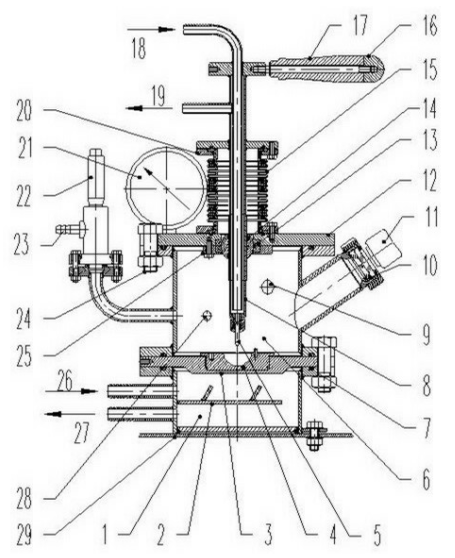
\includegraphics[scale=0.85]{../img/TCpiecschemat}}
\caption{Schemat pieca łukowego. 1- chłodnica, 2- rozdzielacz przepływu, 3- stół topniczy, 4- zimny tygiel, 5- elektroda dodatnia??, 6- komora topienia, 7- pierścień uszczelniający, 8- uchwyt elektrody, 9-wyjcie pompy próżniowej, 10- wziernik kontrolny, 11- lampa, 12- pokrywa komory topienia, 13- teflonowe pierścienie ślizgowe, 14- Teflonowa prowadnica kulowa,  15- miech teflonowy, 16- nakrętka żołądziowa, 17- rękojeść uchwytu anody, 18- doprowadzenie wody do chłodzenia, 19- Odpływ wody chłodzącej, 20- pierścień dzielony, 21- manowakuometr, 22- zawór dozujący, 23- doprowadzenie gazu szlachetnego, 24- szybkozłącze śrubowe, 25- pierścień dociskowy, 26-  doprowadzenie wody chłodzącej 2, 27- odpływ wody chłodzącej, 28- zawór bezpieczeństwa, 29- stół.}
\label{fig:schematPieca}
\end{figure}

\newpage
\begin{figure}[h]
\centerline{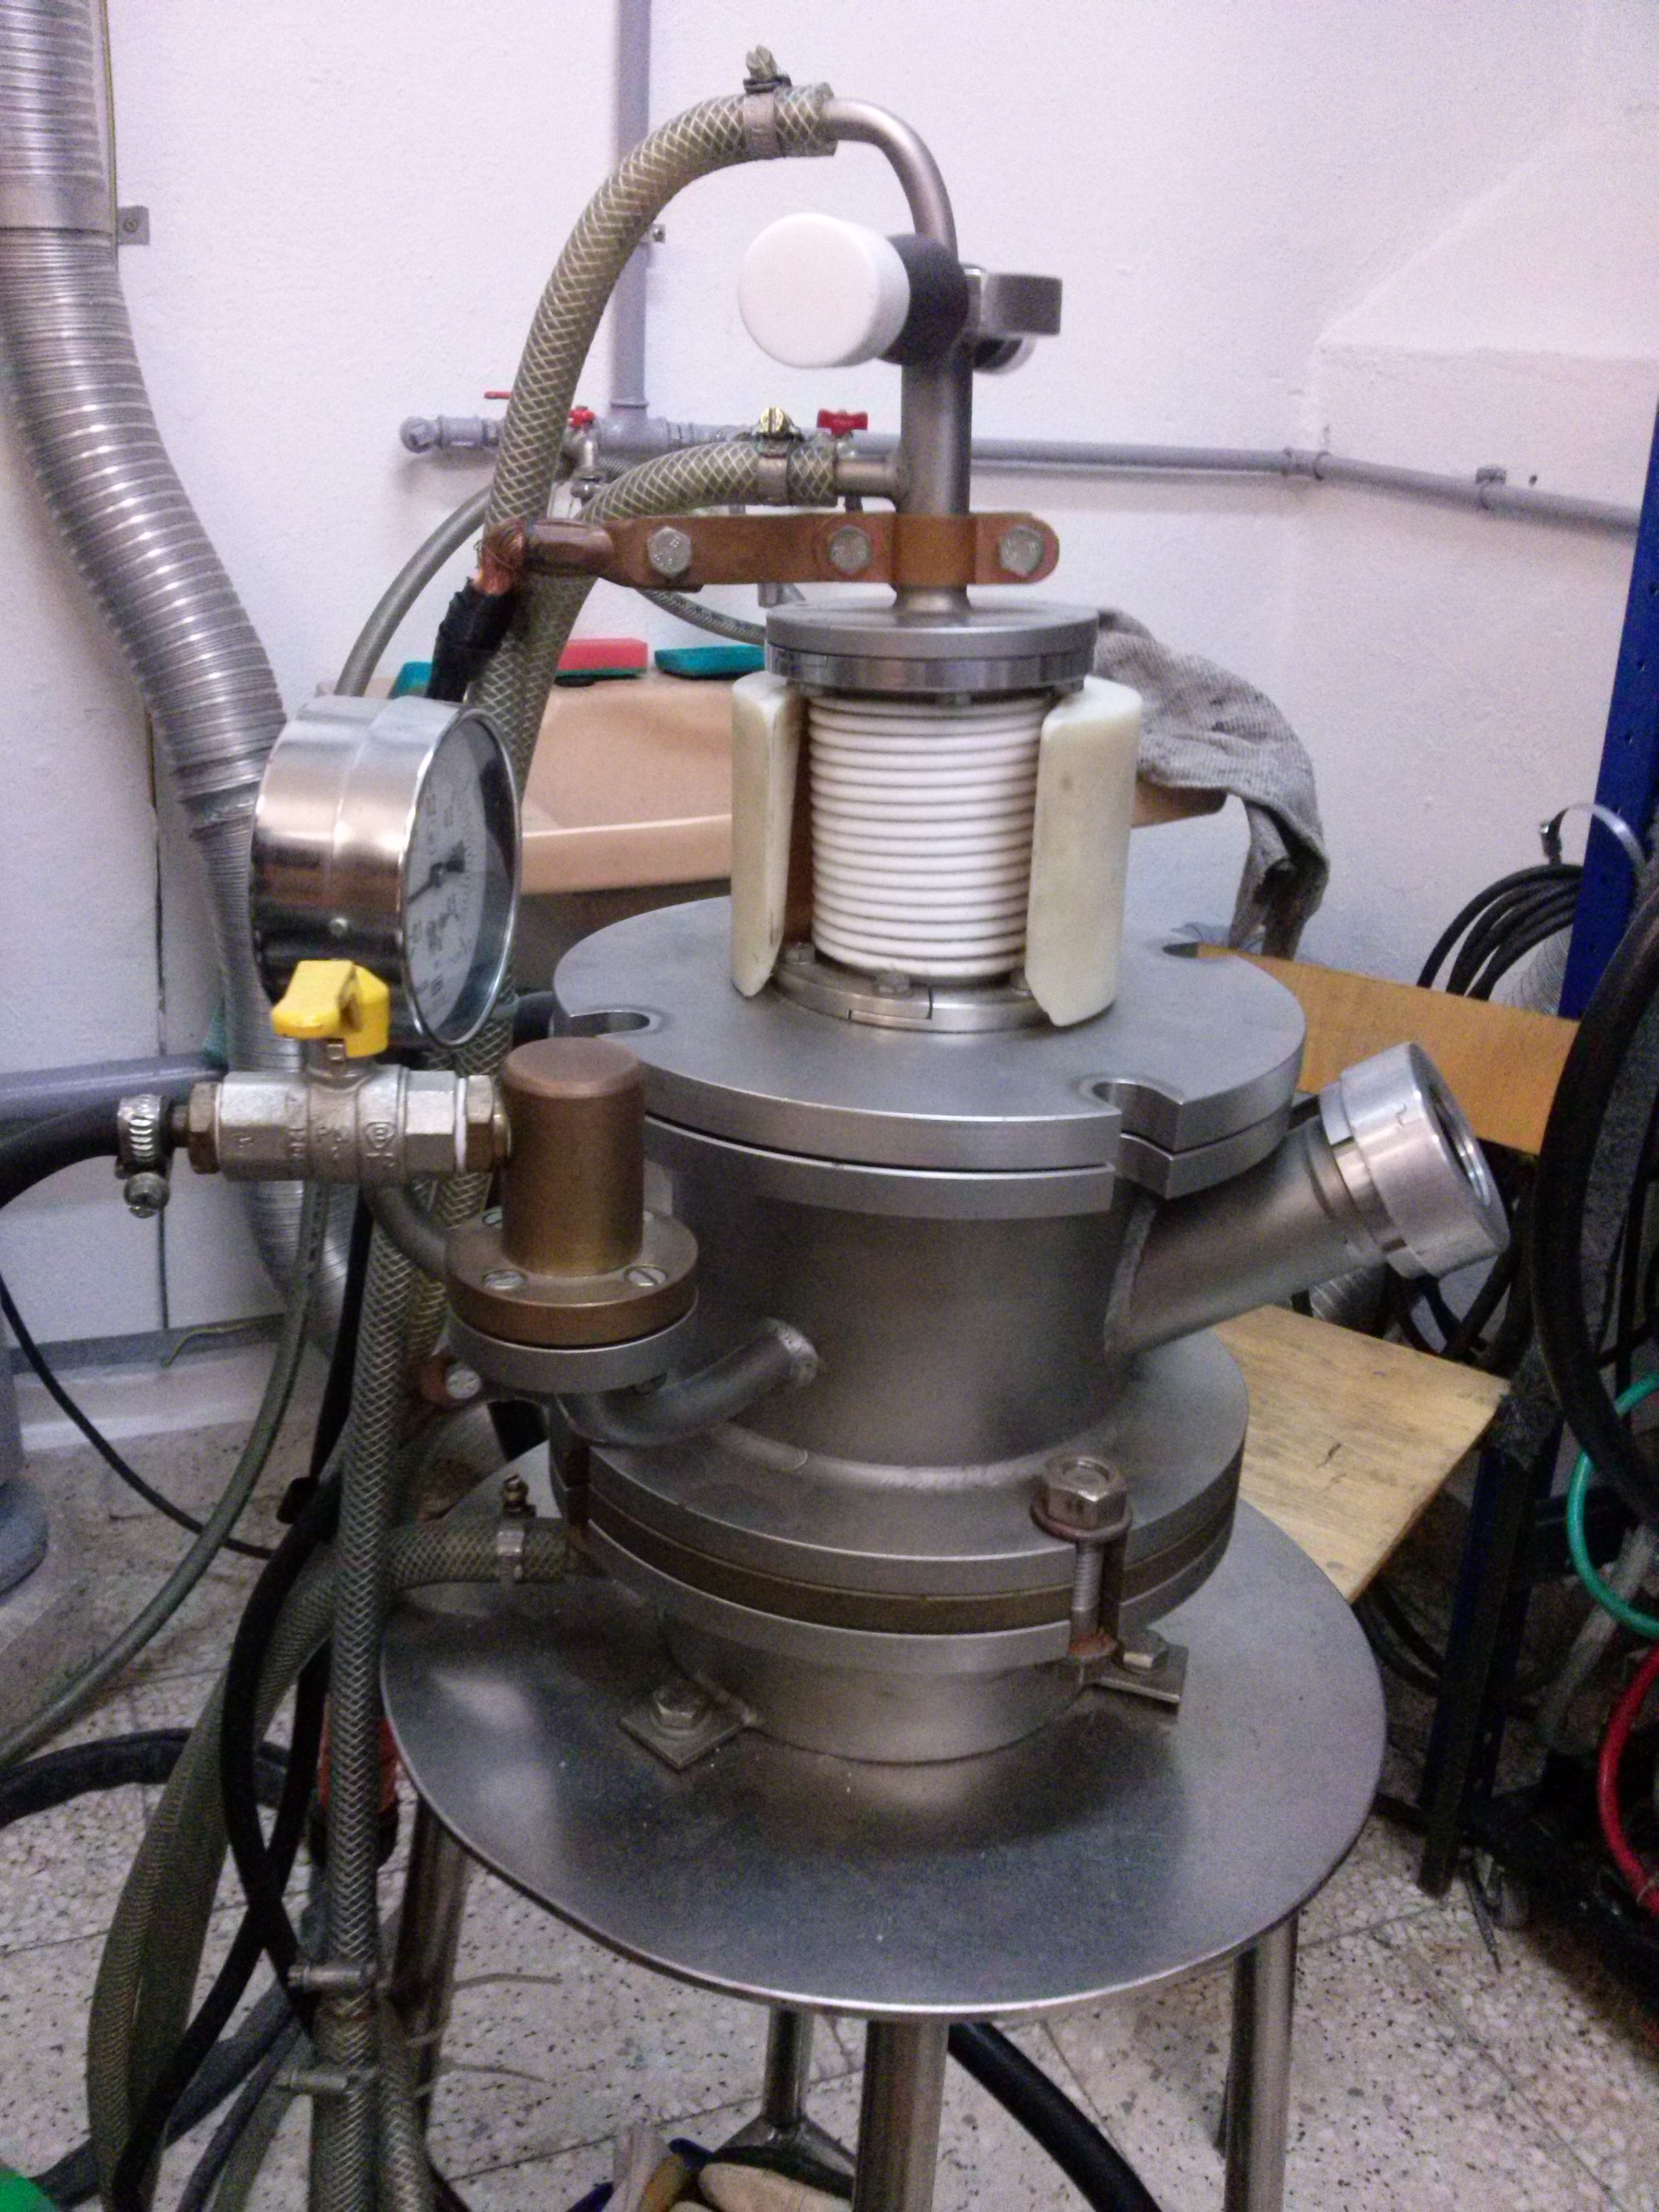
\includegraphics[scale=0.1]{../img/piecfoto}}
\caption{Zdjęcie pieca łukowego z bezdotykowym zapłonem}
\label{fig:fotoPieca}
\end{figure}
 

Kolejność ułożenia pierwiastków w kuwecie pieca łukowego, która jest 
jednocześnie anodą nie może być przypadkowa. Na dole powinien znaleźć się metal ziemi rzadkiej, a na nim 
żelazo, które ma wyższą temperaturę parowania. Sam proces topienia powinien przebiegać bardzo szybko, by 
czas parowania pierwiastków był jak najmniejszy.  Podnosząc natężenie prądu na zasilaczu zwiększamy 
łuk, co umożliwia topienie. Przed procesem topienia należy trzykrotnie odpompować powietrze z komory topienia  i przepłukać 
piec argonem, a następnie uzupełnić jego ilość w piecu do poziomu ciśnienia atmosferycznego. W czasie 
topienia należy pamiętać o przestrzeganiu zasad BHP. Obowiązkowe jest zakładanie fartucha laboratoryjnego, 
rękawic oraz okularów ochronnych. Dopiero tak przygotowani możemy przystąpić do topienia. Wymagana jest 
też obecność drugiej osoby, gdyż piec musi obsługiwać dwoje ludzi. Po przetopieniu próbkę należy wyciągnąć i 
zważyć, by sprawdzić ile ze zważonego metalu ziemi rzadkiej odparowało. Następnie całą procedurę topienia 
musimy powtórzyć oraz zmierzyć ostateczną wagę próbki. Topiąc po raz drugi próbkę należy ustawić tak by 
na górze była strona, którą poprzednim razem próbka była ułożona do spodu. Łatwo to określić, bo obie 
strony różnią się kolorem oraz powierzchnią. Spodnia strona jest gładsza od górnej. Zmiana ułożenia próbki 
ułatwia równomierne przetopienie i zapobiega ewentualnemu pozostaniu dużych, nieprzetopionych 
fragmentów, co trzeba sprawdzić po drugim topieniu. W razie potrzeby topienie należy powtórzyć trzeci raz. 
Stopioną i zważoną próbkę należy wygrzać przez godzinę w temperaturze $800^{\circ}C$ w specjalnie do tego celu 
przygotowanym piecu rurowym. W tym miejscu tak naprawdę próbka nabiera właściwej struktury, zwanej 
fazami Lavesa. %link do sekcji z fazami lawesa
 Atomy zajmują dokładnie te pozycje, w jakich powinny się znaleźć. Tak przygotowane próbki 
należy pociąć. W tym celu używa się piły diamentowej chłodzonej wodą \ref{fig:pila}.

\begin{figure}[h]
\centerline{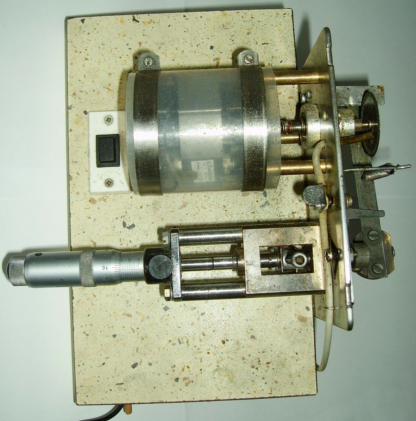
\includegraphics[scale=1]{../img/pila}}
\caption{Piła diamentowa chłodzona wodą}
\label{fig:pila}
\end{figure}



Chłodzenie jest potrzebne, ponieważ 
zarówno piła jak i próbka podczas cięcia mocno się rozgrzewa. Przymocowaną do piły próbkę tnie się 
trzykrotnie w jednej z płaszczyzn, ponieważ potrzebna jest ona do trzech badań: pomiarów oporności, 
magnetostrykcji oraz analizy rentgenowskiej. Cięcia można wykonywać niekoniecznie w takiej kolejności, 
jednak  ważne jest by otrzymane mniejsze próbki były  równoległe, cięcie bez odrywania próbki ułatwia to, 
gdyż nigdy nie uda się ustawić próbki 
idealnie w tej samej pozycji. Cięcie jest w wykonywane ręcznie i należy uważać by zbyt mocno nie dociskać 
tarczy diamentowej do próbki, gdyż grozi to jej zgięciem, a co za tym idzie nierównoległą krawędzią próbki. 
Nierównoległości można wyrównać w późniejszym czasie, jednak wysiłek i czas włożony w to jest 
nieporównywalnie większy niż podczas wolniejszego cięcia. Pierwsza część jest zaokrąglona, więc żeby nie 
tracić niepotrzebnie materiału ucięto ją nieco grubszą: ok 3-4mm od krańca próbki i odłożono do utarcia do 
dyfrakcji rentgenowskiej. Z pozostałej części odcięto 2 cienkie plastry grubości ok. 1-2mm. Jeden z nich, ten 
który posiada mniej porów i niedoskonałości wykorzystano do pomiarów magnetostrykcji, natomiast ostatni 
odcięty kawałek przymocowano do piły w płaszczyźnie poziomej i ponownie bez odrywania przycięto go tak, by 
miała ona kształt cienkiej belki- nie jest to prostopadłościan, ponieważ nie wykonujemy cięć w miejscu 
podstaw. Jest to rzeczą zbędną i  żaden sposób nie płya na pomiar. Głównym założeniem badanej metody jest, by długość belki, a w zasadzie jej 
części, która jest jeszcze prostopadłościanem, był kilkukrotnie większa od jego wymiarów poprzecznych. 
Docelowo belki miały mieć długość ok. 5-8mm, gdyż takie długości otrzymuje się po przetopieniu próbki 7g, 
niestety z powodu małych wymiarów i wiążącej się z nimi delikatnością niektóre ukruszyły się przez co są mniejsze. 

Wspomniana długość jest to odległość między wewnętrznymi złączami, które w późniejszym etapie są 
przymocowywane do próbki i zostanie to opisane w dalszej części pracy. 






%-----------------------------------Przygotowanie do pomiaru opornoci---------------------------------
\subsection{Przygotowanie próbek do pomiarów oporności elektrycznej}

Docięte próbki w kształcie belki zostały wyszlifowane papierem ściernym. Należy używać jak najdrobniejszego papieru, 
ponieważ zbyt gruby, spowoduje  
sytuację odwrotną do pożądanej: zamiast wypolerować,  grube ziarna papieru ściernego mogą pogłębiać 
niedoskonałości, a nawet tworzyć nowe, stąd ponownie zalecana jest cierpliwość i dłuższe polerowanie 
drobniejszym papierem. Podczas przygotowywania próbek do tej pracy korzystano z papieru P-1200 oraz 
P-2000. Następnym krokiem po szlifowaniu jest zmierzenie wymiarów poprzecznych próbki. Powinny być one jak 
najmniejsze. Badane próbki miały poprzeczne wymiary w granicach 1.5-2.5mm. Do pomiarów oporności 
wykorzystuje się metodę czteropunktową. Jest ona bardziej dokładna od zwykłej metody dwupunktowej. W 
tym celu należy przymocować do próbki 4 druciki- po dwa na krajach próbki, ale jeszcze w miejscu, gdzie 
próbka ma kształt prostopadłościanu. Pomiędzy przymocowanymi drucikami nie powinno być żadnych ukruszeń, 
pęknięć ani zwężeń. Wygodnie jest, by druciki przymocowywać w przeciwnych kierunkach. Parę zewnętrzną 
kierujemy w jedną stronę, natomiast wewnętrzną w drugą. Optymalne ułożenie złącz na próbce przedstawia 
rysunek \ref{img:druciki}.

\begin{figure}[!ht]
    \centering
    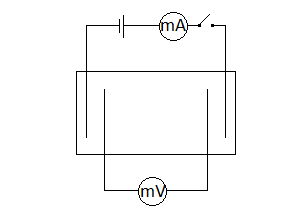
\includegraphics[width =0.8\textwidth]{../img/druciki}
    \caption{Metoda czterokońcówkowa pomiaru oporności elektrycznej}
    \label{img:druciki}
\end{figure}

 W tej pracy stosowano druciki o grubości 0,14mm. Przymocowywane były one do próbki za 
pomocą spawania grafitem. Jest to bardzo łatwa i tania metoda, pozwalająca jednocześnie na precyzyjną 
pracę, co jest rzeczą pożądaną w tym przypadku ze względu na małe wymiary próbek. Do spawania za 
pomocą grafitu wystarczą zasilacz lub akumulator 7V oraz rysiki grafitowe. Przy spawaniu należy uważać, gdyż 
zarówno próbka jak i rysik nagrzewają się do wysokich temperatur. Mocowanie drucików do próbki można 
wzmocnić klejem cyjanoakrylowym. Przydaje się to przy mocowaniu próbki ze złączami na aparaturze 
pomiarowej. Badań dokonuje się w zakresie temperatur od 0K do 800-1000K (w zależności od 
próbki). Ze względu na tak szeroki zakres temperatur pomiarów dokonuje się na dwóch różnych aparaturach w zakresach 0-300K (pomiary niskotemperaturowe) 
oraz 300-800K (pomiary wysokotemperaturowe). Po pomiarach niskotemperaturowych procedurę klejenia próbek trzeba 
przeprowadzić ponownie, gdyż druciki ulegają zniszczeniu lub odklejają się od próbki. W praktyce ciężko umocować 
druciki idealnie prostopadle do krawędzi próbki, dlatego wylicza się srednią odległosć między drucikami, Przykładowe
zdjęcie próbki z przymocowanymi drucikami przedstawia rysunek \ref{probkaOpor}.

\begin{figure}[h]
    \centering
    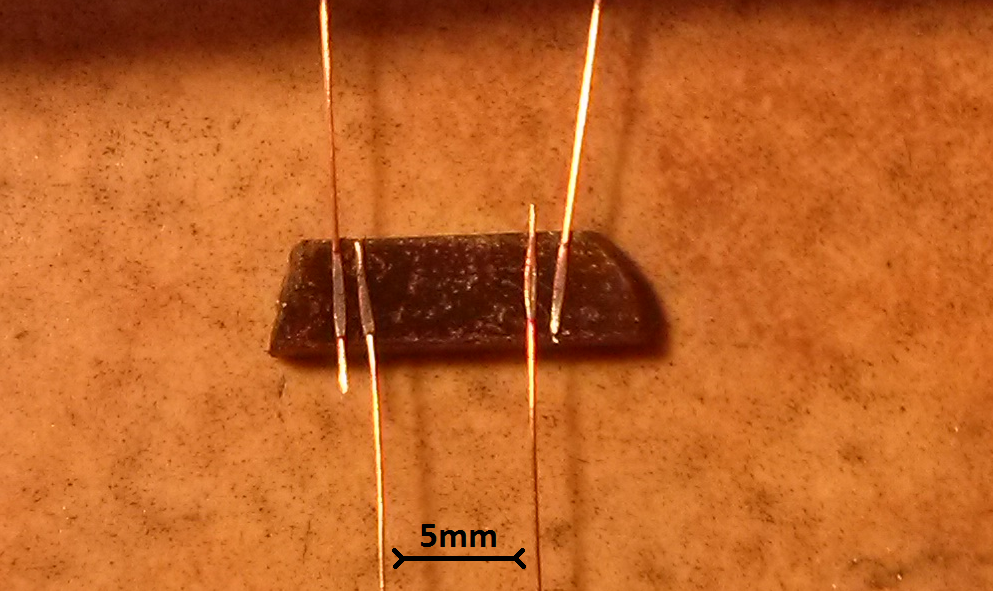
\includegraphics[width =0.7\textwidth]{../img/probkaOpor}
    \caption{Próbka do pomiaru opornosci z przymocowanymi końcówkami}
    \label{probkaOpor}
\end{figure}

Schemat aparatury do pomiarów wysokotemperaturowych przedstawia rysunek \ref{img:schematUkl} 

\begin{figure}[h]
    \centering
    \includegraphics[width =1.0\textwidth]{../img/schemat}
    \caption{Schemat układu pomiarowego do badania oporności w wysokich temperaturach: 1 - zasilacz, 2 - komutator, 3 -
I [mA], 4 - U [mV], 5 - T[K], 6 - piec rurowy, 7 - automatyczny regulator temperatury, 8 - komputer, 9 - pompa próżniowa}
    \label{img:schematUkl}
\end{figure}

Aparatura pomiarowa składa się z pieca rurowego [6], w którym umieszczona jest próbka przymocowana do sondy i 
umieszczona w szklanej rurze, w której panuje próżnia wytwarzana za pomocą pompy próżniowej [9]. Stan próżni jest 
wymagany, by nie doszło do pęknięć szkła. Z sondy pomiarowej odchodzą trzy pary złącz: prądowe -  przymocowane do próbki 
(złącza zewnętrzne na rysunku \ref{img:druciki}, napięciowe- para wewnętrzna na tym samym rysunku.Trzecią parą są 
połączone w jedną wtyczke 
złącza termopary, której końcówka zamocowana jest przy samej próbce. Należy sprawdzić ułożenie wtyczki. Źle włożona 
pokazuje temperaturę odwrotnie-maleje gdy piec jest włączony, co uniemożliwia pomiar cykliczny, gdyż program czeka, 
aż wartoć temperatury będzie większa o minimum $5^{\circ}C$ od poprzednio zanotowanego pomiaru. Każde z tych 
złącz podpięte jest do osobnego 
multimetru: wyjście prądowe - multimetr [3],  napięciowe - multimetr [4], termopara - multimetr [5]. Prąd na próbkę podawany jest 
z zasilacza [1] po przejciu przez komutator [2]. Dane ze wszystkich trzech 
multimetrów [3,4,5]  przekazywane są do komputera [8]. Za regulację temperatury odpowiada regulator [7].  Napisany w Javie 
dokładnie do takiego układu pomiarowego program 
zczytuje i przelicza otrzymane dane. Użytkownik ma możliwosć wykonania pojedynczego pomiaru, jednak z 
doswiadczalnego punktu widzenia bardziej interesujące jest wykonanie serii pomiarów. Oprogramowanie pozwala na 
wykonanie pomiarów w okrelonych odstępach czasu lub temperatury. Dokonując pomiarów do tej pracy korzystano, jak 
już wspomniano z 
drugiej opcji. Po zakończeniu pomiaru należy zapisać zebrane dane, tzn. temperaturę, napięcie i prąd na próbce, 
opór, czas (wyorzystywany przy pomiarach w odstępach czasu) oraz zmianę oporu w funkcji temperatury do pliku 
wynikowego. Obróbki tych danych dokonuje się w programie OriginPro  dostępnym w laboratorium. W pierwszej 
kolejnosci należy z wartości oporu wyliczyć oporność  przez proste przekształcenie:

  \begin{equation}
    \rho=R\frac{ab}{l}
    \label{opornosc}
  \end{equation}

gdzie $\rho$ to opornosc własciwa, $R$ opór, $a$ i $b$ to wymiary poprzeczne próbki, $l$ odległosc między 
wewnętrzymi złączami. 


 Analogicznego przeszktałcenia należy wykonać z pomiarami nistkotemperaturowymi, a następnie je połączyć. Dane umieszcza się 
na wykresie. Przykładowa zawartosć pliku wyjsćiowego ukazana jest w dodatku  \ref{plik}.


%--------------------------------Przygotowanie do pomiarów magnetostrykcji---------------------------
\subsection{Przygotowanie do pomiarów magnetostrykcji}

Przygotowanie próbek do pomiarów magnetostrycki, które zostały wykonane dodatkowo w ramach pracy jest całkowicie 
odmienne. W tym przypadku zależy nam, by uzystać jak największą powierzchnię bez jakichkolwiek nierównosci, pęknięć 
lub jakichkolwiek innych uszkodzeń. Wymaga to wiele czasu i cierpliwosci, gdyż tak jak wspominano pracę należy 
wykonać jak najdrobniejszym papierem sciernym. Na wypolerowaną powierzchnię próbki przyklejamy zgodnie z 
instrukcją producenta tensometr foliowy. Specjalny klej schnie ok. 24 godziny i w tym czasie próbka jest scisnięta w
imadle. Po upływie tego czasu próbka jest gotowa do przymocowana na sondzie.

%------------------------------Metody pomiarowe------------------------------------------------
\section{Metody pomiarowe}




%---------------------------------Badania dyfrakcyjne------------------------
\subsection{Metoda proszkowa Debye'a-Scherrera-Hulla}

Podstawową metodą badania substancji polikrystalicznych jest metoda Debye'a-Scherrera-Hulla (DSH) przy pomocy monochromatycznego
promieniowania rentgenowskiego. Próbka taka składa się z tysięcy bezładnie ułożonych krystalitów wielkości  0,1 - 10 $\mu$m. Ułożenie
takie sprawia, że różne są kąty $\theta$ padania promieni wiązki na poszczególne krystality. Refleks uzyskuje się wyłącznie od tych płaszczyzn krystalograficznych krystalitów, które spełniają równanie Bragga:

  \begin{equation}
    n\lambda = 2d\sin\theta
    \label{eq:bragg}
  \end{equation}

gdzie n jest rzędem refleksu, $\lambda$ długością promieniowania, d odległością między płaszczyznami a $\theta$ kątem padania promieni na krystality.

Otrzymane refleksy tworzą kąt $2\theta$ z pierwiotną wiązką i leżą na tworzącej stożka, którego kąt rozwarcia jest 2 razy większy 
od kąta $2\theta$. Wszystkie refleksy, które mają ten sam rząd i odległość międzypłaszczyznową $d$ układają się na tworzącej 
jednego stożka. Reflesky od płaszczyzn o innej wartości parametru $d$ układają się na tworzącej innego stożka. Na płaskiej, 
prostopadłej do padającego promieniowania błonie fotograficznej uzyskuje się jako wynik przecięcia z tworzącymi stożków ciągłe 
okręgi. Refleksy otrzymane w tej sposób nazywane są debajogramami. Mierząc promienie otrzymanych okręgów i znając odległość 
próbki od błony fotograficznej uzyskuje się wartość kąta $2\theta$:

   \begin{equation}
    \tg2\theta= \frac{r}{D}
    \label{eq:bragg}
  \end{equation}

gdzie r jest promieniem okręgu debajowskiego a D odległością próbki od błony fotograficznej.

Płaskie błony fotograficzne umożliwiają pomiary refleksów dla $\theta < 30^{\circ}$ oraz refleksów zwrotnych dla
$\theta > 60^{\circ}$. Ograniczenia takiego nie posiadają kamery cylindryczne, w których błona fotograficzna znajduje się na 
okręgu o środku w miejscu próbki. średnice kamer cylindrycznych są tak dobierane, by 1mm na błonie fotograficznej odpowiadał 
$1^{\circ}$ lub $2^{\circ}$. Poddając błonę fotograficzną obróbce fotochemicznej otrzymuje się krzywe czwartego rzędu
zwane prążkami dyfrakcyjnymi. otrzymane linie mają charakter ciągly, lub nieciągły w zależności od tego, czy w badanej objętości 
preparatu na którą pada wiązka promieniowania znajduje się wystarczająca liczba krystalitów bądź nie. W przypadku gdy jest ich
zbyt mało ciągłość można otrzymać przez obrót próbki do pozycji w której będzie większe prawdopodobieństwo uzyskania refleksów od większej liczy krystalitów.

Bieg promieni w goniometrze dyfraktometru polikrystalicznego przedstawia rysunek \ref{biegPromieni}:

\begin{figure}[h]
\centerline{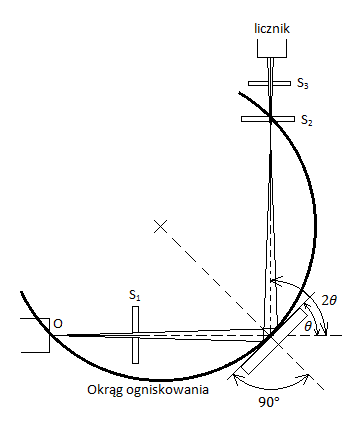
\includegraphics[scale=1]{../img/biegPromieni}}
\caption{Biegr promieni w goniometrze: O - ognisko lampy, $S_1$,  $S_2$,  $S_3$ - szczeliny}
\label{biegPromieni}
\end{figure}


Wiązka promieniowania rentgenowskiego, która wydostaje się z lampy trafia do goniometru, gdzie w specjalnym układzie
szczelin zostaje uformowana, następnie pada na próbkę, a otrzymane refleksy zostają odprowadzone do licznika ponownie
przechodząc przez układ szczelin.

Ognisko lampy rentgenowskiej, próbka w kształcie płytki oraz szczelina $S_{2}$ znajdują się na okręgu ogniskowania, który jest 
zmienny, co wywołane jest przez ruch detektora.

Dużą rolę w tej metodzie odgrywa sposób przygotowania badanego preparatu. Powtarzalne wyniki otrzymuje się dla wielkości 
krystalitów mniejszych niż $10\mu$m, dlatego odcięty fragment próbki umieszcza się w moździeżu agatowym, zalewa spirytusem
bezwodnym i uciera. Spirytus zabezpiecza przed ewentualnymi iskrami, które mogą się wytworzyć podczas tarcia niektórych 
próbek. Ucieranie powinno trwać jak najdłużej, mniej więcej ponad 30 minut. Najlepiej ucierać próbkę przez kilka minut jeszcze po 
tym gdy patrząc pod swiatło na nią nie widzimy żadnym błyszczących się elementów.Tak utartą próbkę umieszcza się w kuwecie
pomiarowej dbając o to, by preparat miał płaską i gładką powierzchnię. a następnie na drodze promieni rentgena. 

W pomiarach używano lampy molibdenowej, która wzbudza atomy 
Itru, przez co na jego  dyfraktogramie widoczne jest dosć wysokie tło. Pomiarów dokonywano w trybie czasowym w 
zakresie  kątowym $2\theta$  $10^{\circ}-60^{\circ}$ co $0,05^{\circ}$. Cały pomiar trwał ok 3 godzin. 

%---------------------------Metoda pomiaru oporności-------------------------------------------------
\subsection{Metoda pomiaru oporności właściwej}
Oporność elekttyczną związków międzymetalicznych, które posiadają uporządkowanie magnetyczne, opisuje reguła
Matthiesena:

  \begin{equation}
    \rho(T)=\rho_m(T)\rho{_f}(T)+\rho_0
    \label{Matthiesen}
  \end{equation}
  
Zgodnie z tą regułą oporność właściwa  $\rho$ takich związków zależy od trzech czynników, którymi są: $\rho_m(T)$ jest opornością
związaną z rozpraszaniem na momentach magnetycznych, $\rho_f(T)$ rozpraszaniem elektronów związancyh z drganiami sieci 
krystalicznej, a $\rho_0$ jest opornością resztkową.

Oporność $\rho_f$ dana jest zależnością $Blocha-Grne\"{u}isena$:

  \begin{equation}
    \rho{_f}(T)=R{_t}\left(\frac{T}{\theta}\right){^5}
		\int_o^\frac{\theta}{T}
		\frac{{z^5}dz}{(e^z-1))(1-e^{-z})}
    \label{ro_wlasciwe_fononowe}
  \end{equation}
  
  gdzie $R_t$ jest stałą temperaturową, a $\theta_D$ temperaturą Debye'a.
  Zależność tą dla niskich temperatur (T<<$\theta_D$) można zapisać jako:
  
  \begin{equation}
    \rho{_f}(T)=497,5R{_t}\left(\frac{T}{\theta}\right){^5}
    \label{ro_wlasciwe_fononowe_niskie}
  \end{equation}
  
natomiast dla temperatur wysokich (T>>$\theta_D$) redukuje się do:

  \begin{equation}
    \rho{_f}(T)=R{_t}\frac{T}{\theta}
    \label{ro_wlasciwe_fononowe_wysokie}
  \end{equation}
  
Drugi człon $\rho_m$ który wynika z rozpraszania na momentach magnetycznych można zapisać w niskich temperaturach
(T<<$T_C$) wzorem:

 \begin{equation}
    \rho_m=A_2T^2+A_1T
    \label{ro_m_niskie}
 \end{equation}
 gdzie $A_2$ i $A_1$ to stałe temperaturowe.
 
W wysokich temperaturach (T>>$T_C$) momenty magnetyczne całkowicie tracą uporządkowanie, stąd stąd $\rho_m$ jest stałą
niezależną od temperatury.

Łącząc równania \ref{Matthiesen}-\ref{ro_m_niskie} otrzymujemy następujące zależności. Dla temperatur niskich
(T<<$\theta_D$ i T<<$T_C$) $\rho(T)$ wynosi:

  \begin{equation}
    \rho(T)=497,5R{_t}\left(\frac{T}{\theta}\right){^5}
		+A_2T^2+A_1T+\rho_0
    \label{ro_niskie}
  \end{equation}
  
W wysokich temperaturach (T>>$\theta_D$ i T>>$T_C$) $\rho(T)$ przyjumuje postać:

  \begin{equation}
    \rho=497,5R{_t}\left(\frac{T}{\theta}\right)
		+A_3
    \label{ro_wysokie}
  \end{equation}
  
  gdzie $A_3$ jest stałą temperaturową.
  

Analiza numeryczna zebranych wyników polega na zamianie oporu $R(T)$ na oporność przez proste przemnożenie przez
iloczyn wymiarów próbki:

  \begin{equation}
    \rho(T)=R(T)\frac{ab}{l}
    \label{opor->opornosc}
  \end{equation}

  gdzie $a$ i $b$ są długościami boków najmmniejszej ściany próbki a $l$ długością najdłuższej krawędzi próbki.
Następnie do tak przygotowanych na podstawie wzorów \ref{ro_niskie}-\ref{ro_wysokie} należy w niskich temperaturach
dopasować wielomian piątego stopnia, natomiast dla temperatur wysokich prostą. Wstawiając współczynniki wyznaczone
podczas dopasowania do tych wzorów pozwalają na wyznaczenie wartości $R_t$ oraz$\theta_D$. Posiadając wspomniane wielkości
wyznacza się $\rho_0, \rho_m(T) oraz \rho_f(T)$.

W celu wyznaczenia temperatury Curie $T_C$ badanej serii próbek należy skorzystać z wyliczonej poprzednio oporności
związanej z rozpraszaniem na momentach magnetycznych $\rho_m(T)$. Obliczając zmianę wartości tego przyczynku 
w miarę zmiany temperatury $\frac{\Delta\rho_{m}(T)}{\Delta T}$ łatwo zaobserwować, że poniżej temperatury Curie
$T_C$ zmiany są duże, natomiast powyżej $T_C$ nachylenie jest niewielkie. Dla obu tych przedziałów wyznacza się 
proste. Temperatura dla której obie wyznaczone proste przecinają się jest szukaną temperaturą Curie $T_C$.


%----------------------------Metoda pomiaru magnetostrykcji----------------------------------------------
\subsection{Metoda pomiaru magnetostrykcji}

Magnetostrykcja to zjawisko, w którym ciało stałe pod wpływem przyłożonego zewnętrznego pola magnetycznego zmienia swoje wymiary. Magnetostrykcja czyli wielkość odkształcenia jakiemu ulega ciało stałe rośnie wraz ze wzrostem 
wartości pola. W przypadku jednowymiarowym odkształcenie to zapisuje się jako $\lambda=\frac{\Delta l}{l}$. Wielkość odkształcenia rośnie aż do wartości maksymalnej zwanej wartością nasycenia $\lambda_S$. W materiałach polikrystalicznych gdzie ułożenie krystalitów jest przyprzypadkowe dokonuje się pomiarów w dwóch 
kierunkach. Wyróżnia się magnetostrykcję wzdłużną $\lambda_{||}$ która jest mierzona wzdłuż pola i magnetostrykcję poprzeczną $\lambda_{\perp}$ gdzie mierzona jest wartość magnetostrykcji w kierunku prostopadłym do linii pola
magnetycznego. W ogólnym przypadku zmianę objętości ciała stałego wywołaną przez zjawisko magnetostrykcji zwaną magnetostrykcją objętościową określa równanie \ref{magneto_objWz}

  \begin{equation}
 \frac{\Delta V}{V}=\lambda_{||}+2\lambda_{\perp}
 \label{magneto_objWz}
 \end{equation}
  
 Dodatkowo, gdy $\lambda_{\perp}\neq\lambda_{||}$ zmianie ule także kształt ciała. Zjawisko to nazywane jest magnetostrykcją kształtu i wyznacza się ją za pomocą równania \ref{magneto_ksztWz} 
 
 \begin{equation}
 \lambda_{t}=\lambda_{||}-2\lambda_{\perp}
 \label{magneto_ksztWz}
 \end{equation}

Pomiar magnetostrykcji odbywa się przy pomocy tensometru foliowego oporowego, którego mocowanie omówiono 
wczeniej. Przygotowaną próbkę przylutowuje się do sondy, która następnie ląduje we wnętrzu elektromagnesu.
Najważniejsze jest ułożenie próbki wewnątrz: próbka musi leżeć idealnie pododku, gdzie pole jest jednorodne. Oprócz 
wymogu umiejscowienia próbki w samym srodku elektromagnesu muszą być spełnione dodatkowe warunki. Pomiaru 
dokonuje się w dwóch kierunkach: tensometru ułożonego równolegle i prostopadle do lini pola, stąd i o to należy
zadbać. Przyjmuje się, że sonda jest ułożona prostopadle do pola, więc krawędzie tensometru muszą być umieszczone
równolegle do krawędzi sondy



jaki rys?




%------------------------------------------------------------------------------------------
%------------------------------wyniki pomiarów----------------------------------------
%------------------------------------------------------------------------------------------


\section{Wyniki pomiarów}

\subsection{Wyniki pomiarów dyfrakcyjnych}

Poniższe rysunki \ref{Dyrentgen} - \ref{Yrentgen} przedstawiają wyniki pomiarów dyfrakcyjnych wraz z analizą 
przeprowadzoną przy pomocy programu FullProf. Czerwone punkty to dane pomiarowe, czarna linia to wygenerowany 
w FullProfie oczekiwany kształt widma. Zielone pionowe kreski oznaczają punkty w których znajdują się piki dyfrakcyjne, 
a niebieska linia to różnica między natężeniem zmierzonym a wyliczonym przez program.

\newpage
\newgeometry{hmargin={0.5cm, 0.5cm}, height=10.0in}

\newpage
\begin{sidewaysfigure}[htp]
  \centering
  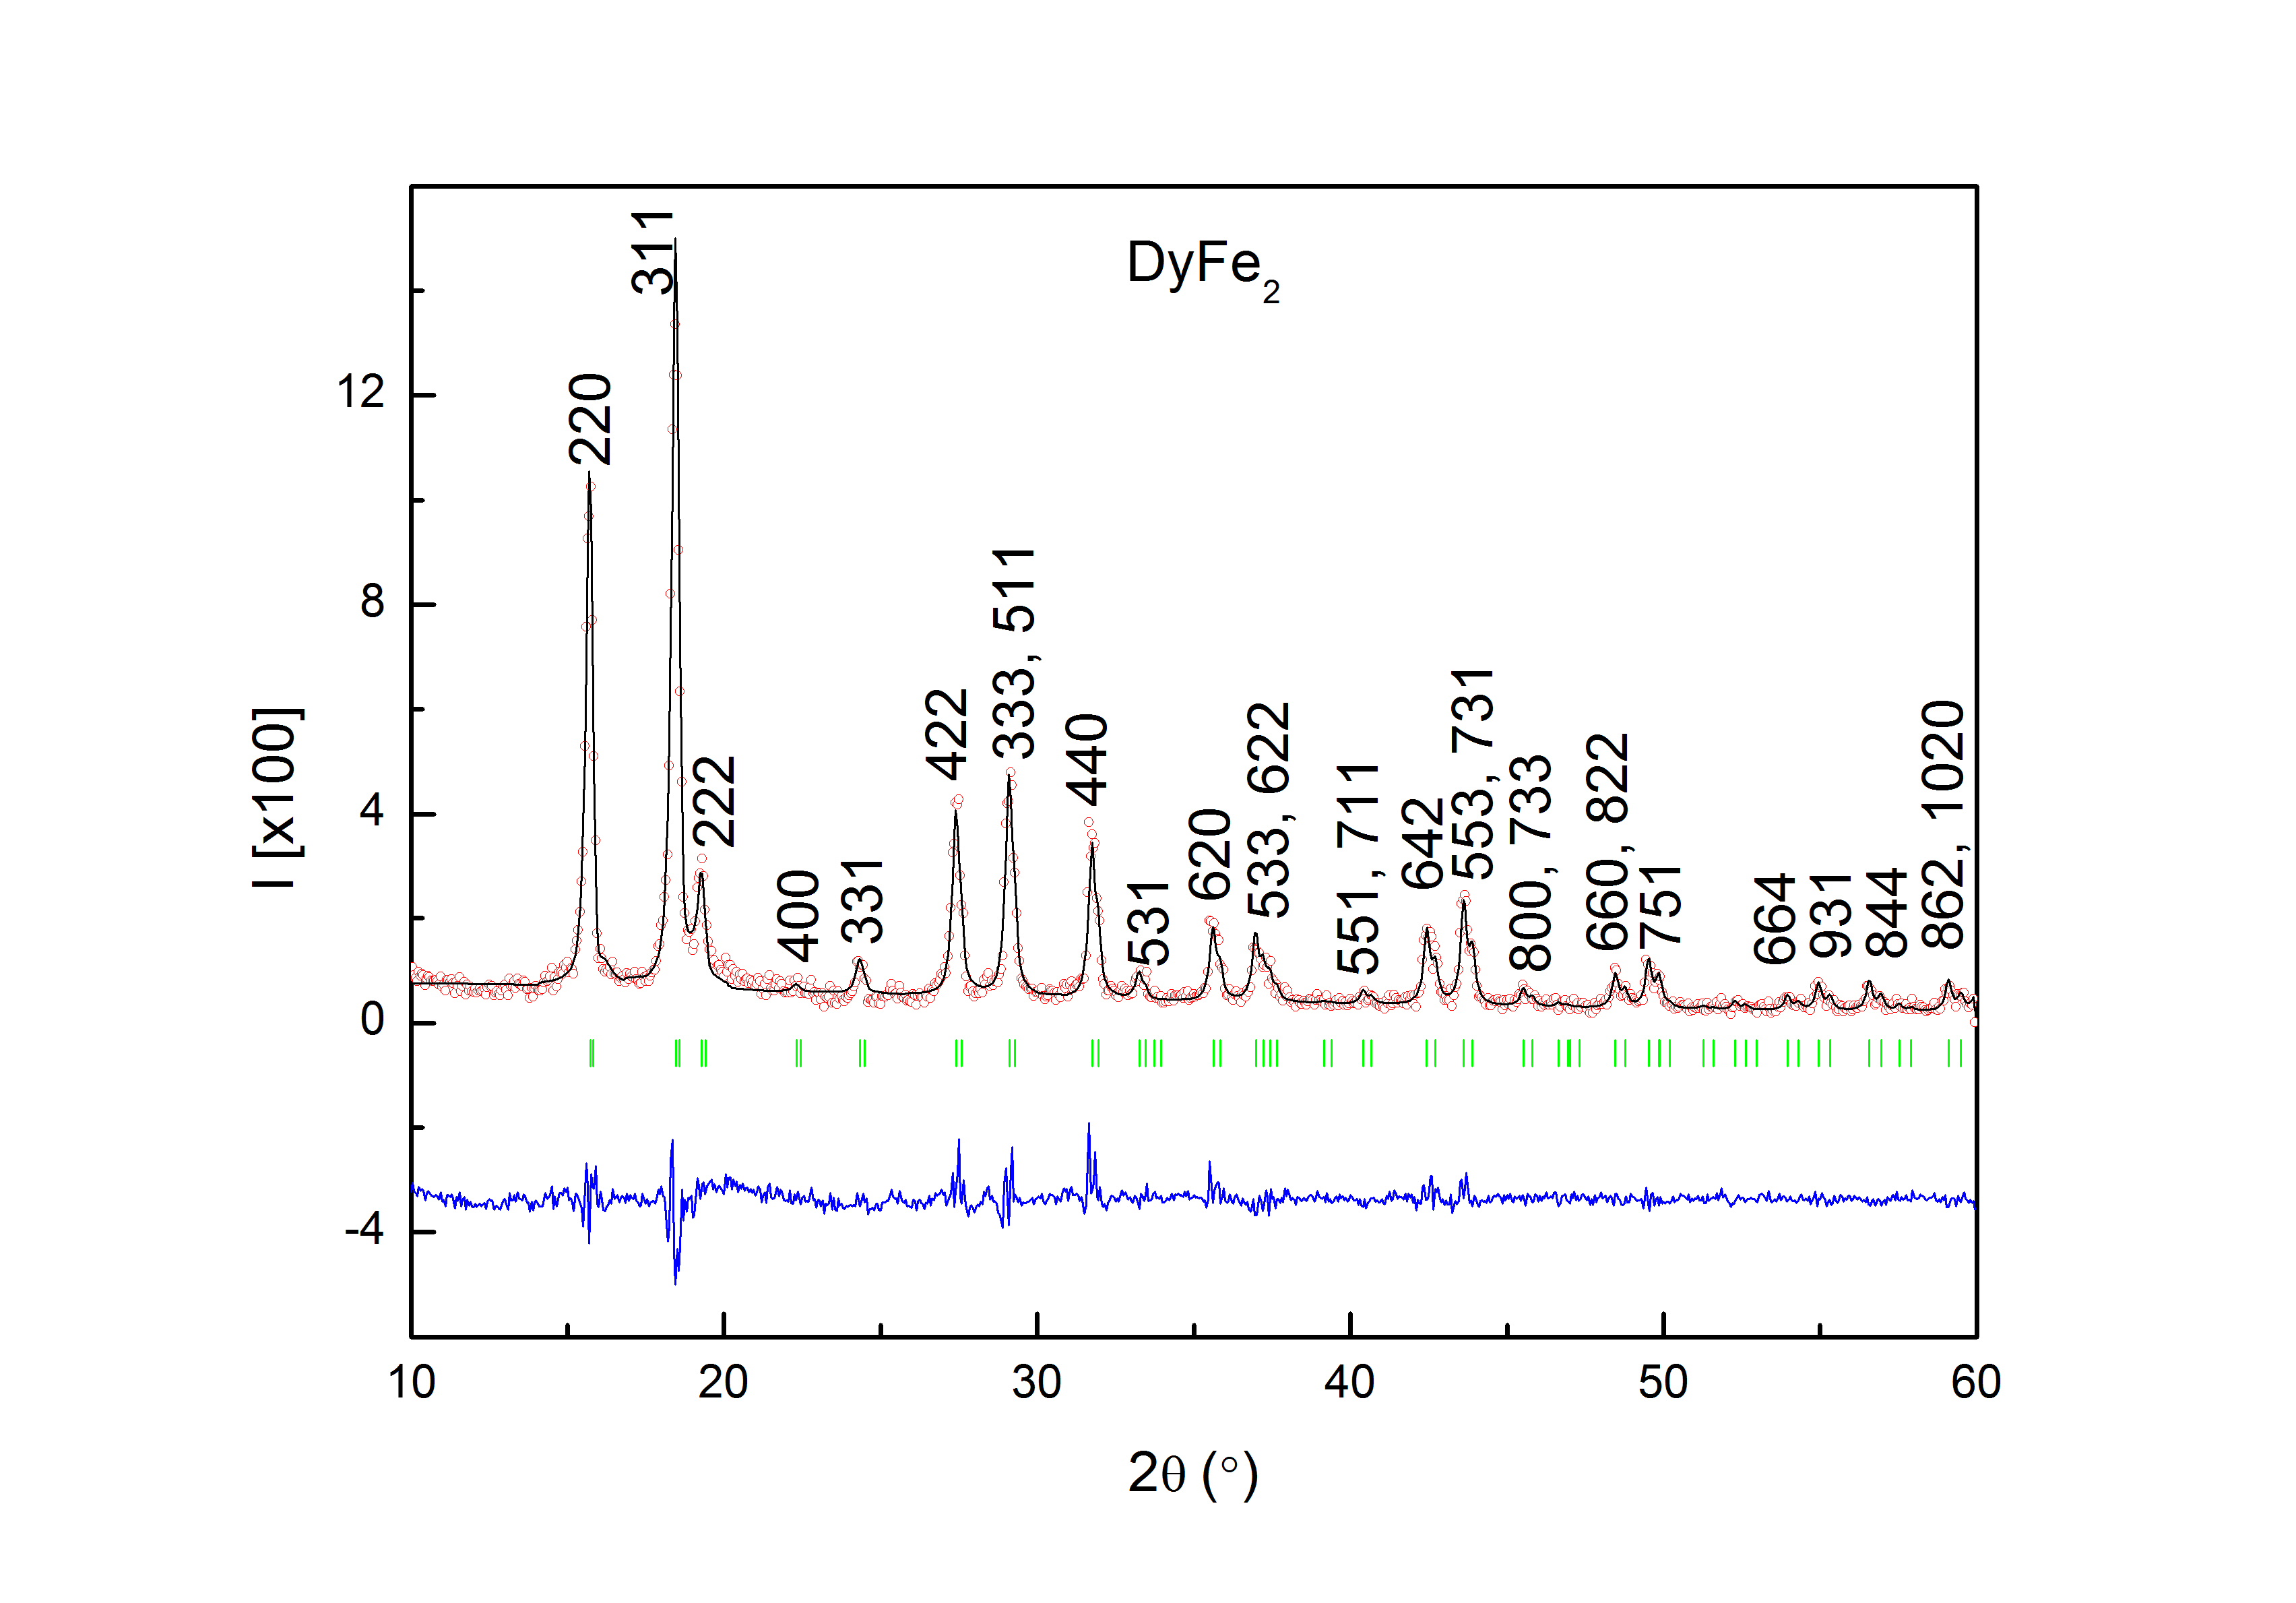
\includegraphics[width=0.85\linewidth]{../img/dif/DyFe2rentgen}
  \caption{Dyfraktogram rentgenowski próbki $\nit{Dy}\nit{Fe}_2$}
  \label{Dyrentgen}
\end{sidewaysfigure}

\newpage
\begin{sidewaysfigure}[htp]
  \centering
  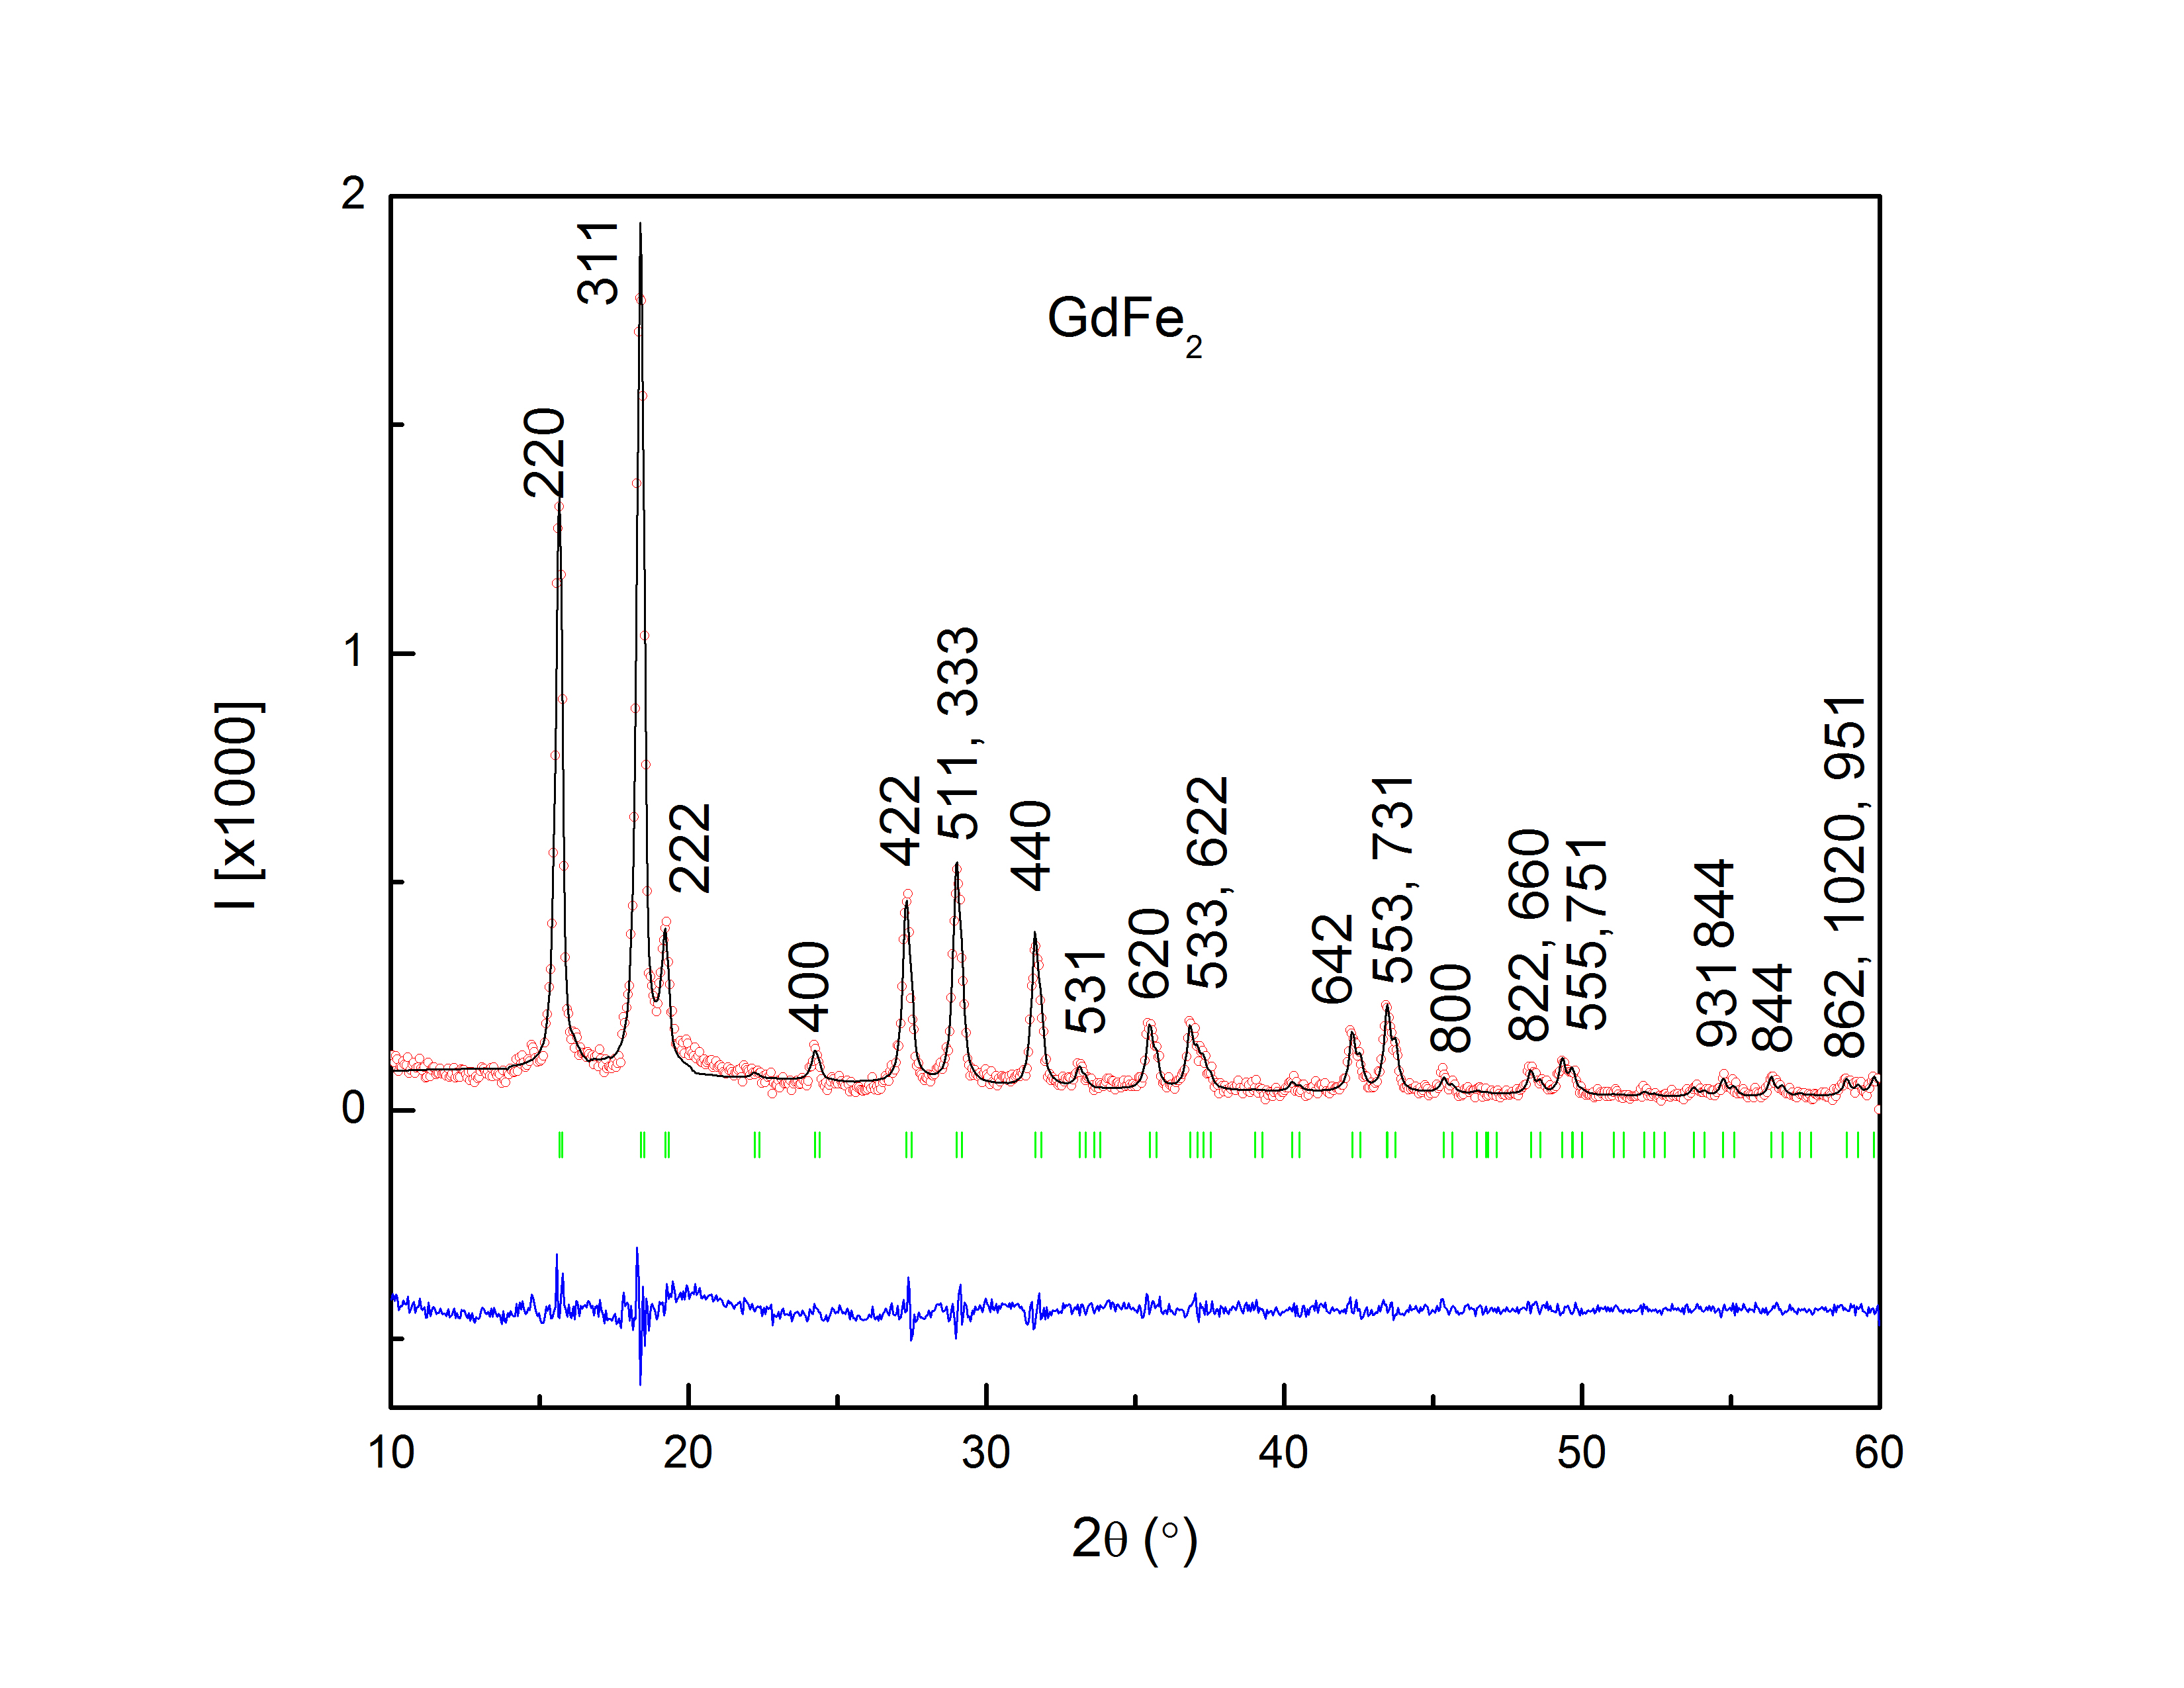
\includegraphics[width=0.8\linewidth]{../img/dif/GdFe2rentgen}
  \caption{Dyfraktogram rentgenowski próbki $\nit{Gd}\nit{Fe}_2$}
  \label{Gdrentgen}
\end{sidewaysfigure}

\newpage
\begin{sidewaysfigure}[htp]
  \centering
  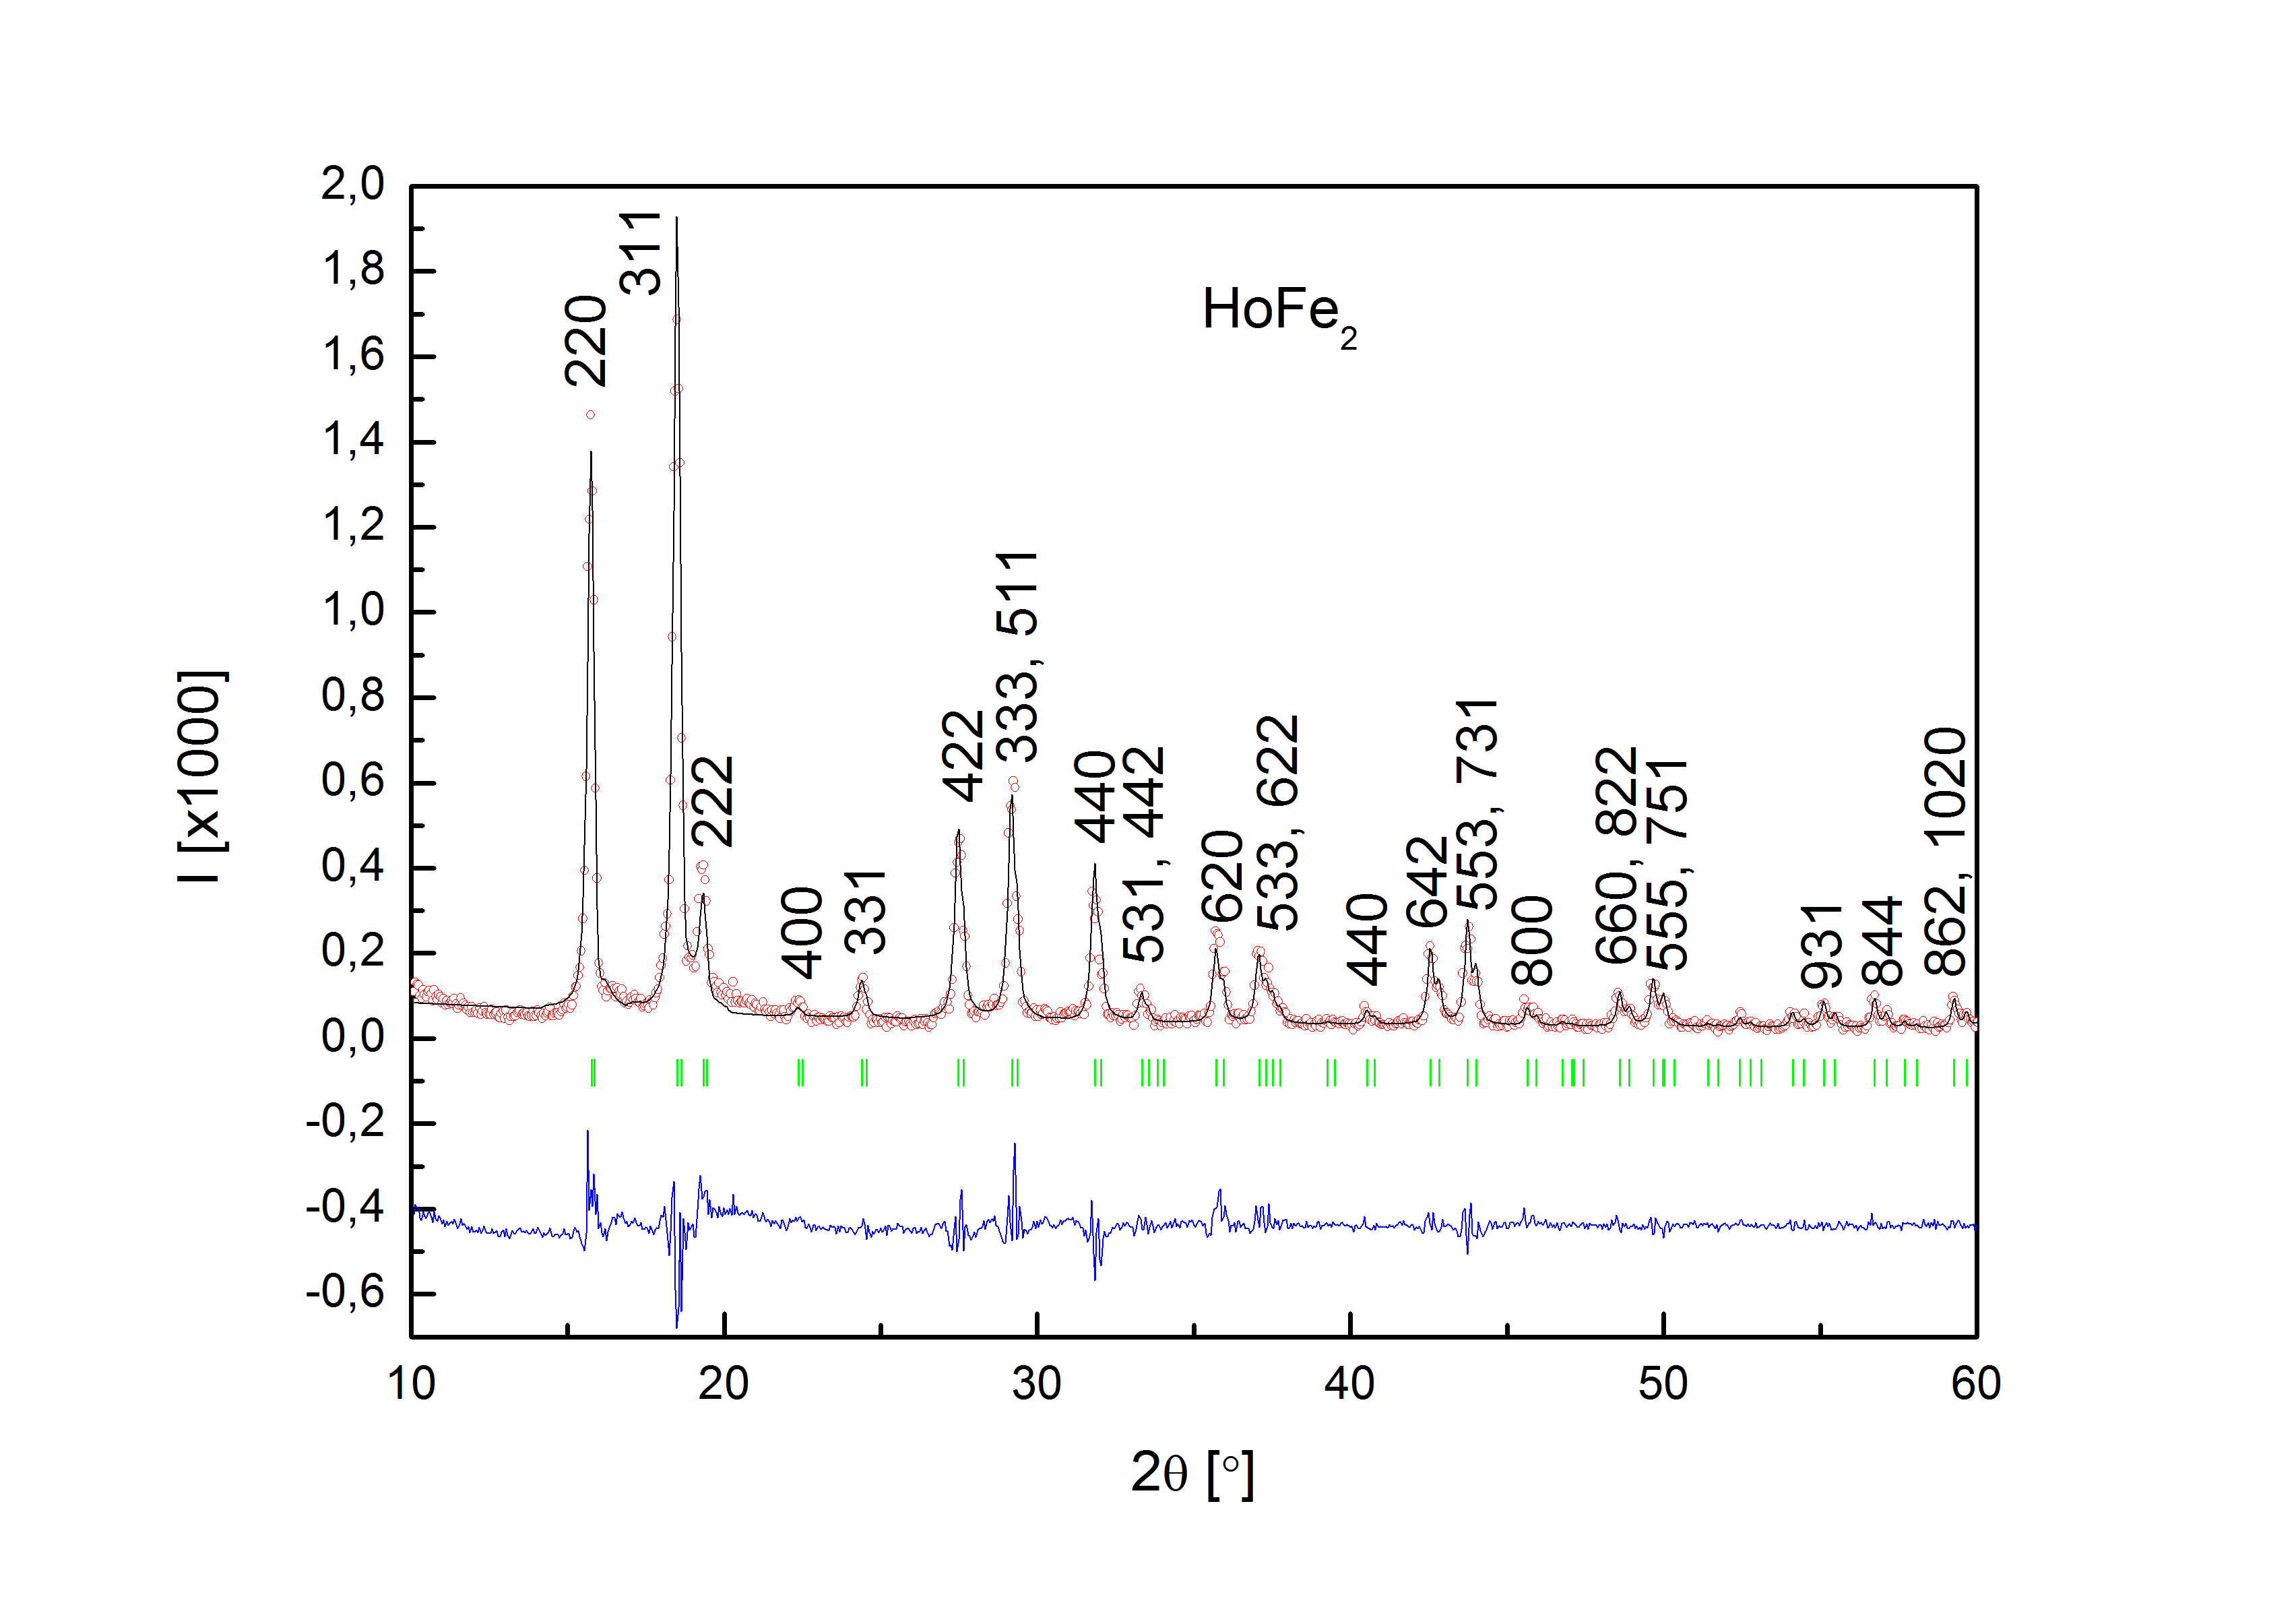
\includegraphics[width=0.85\linewidth]{../img/dif/HoFe2rentger}
  \caption{Dyfraktogram rentgenowski próbki $\nit{Ho}\nit{Fe}_2$}
  \label{Horentgen}
\end{sidewaysfigure}

\newpage
\begin{sidewaysfigure}[htp]
  \centering
  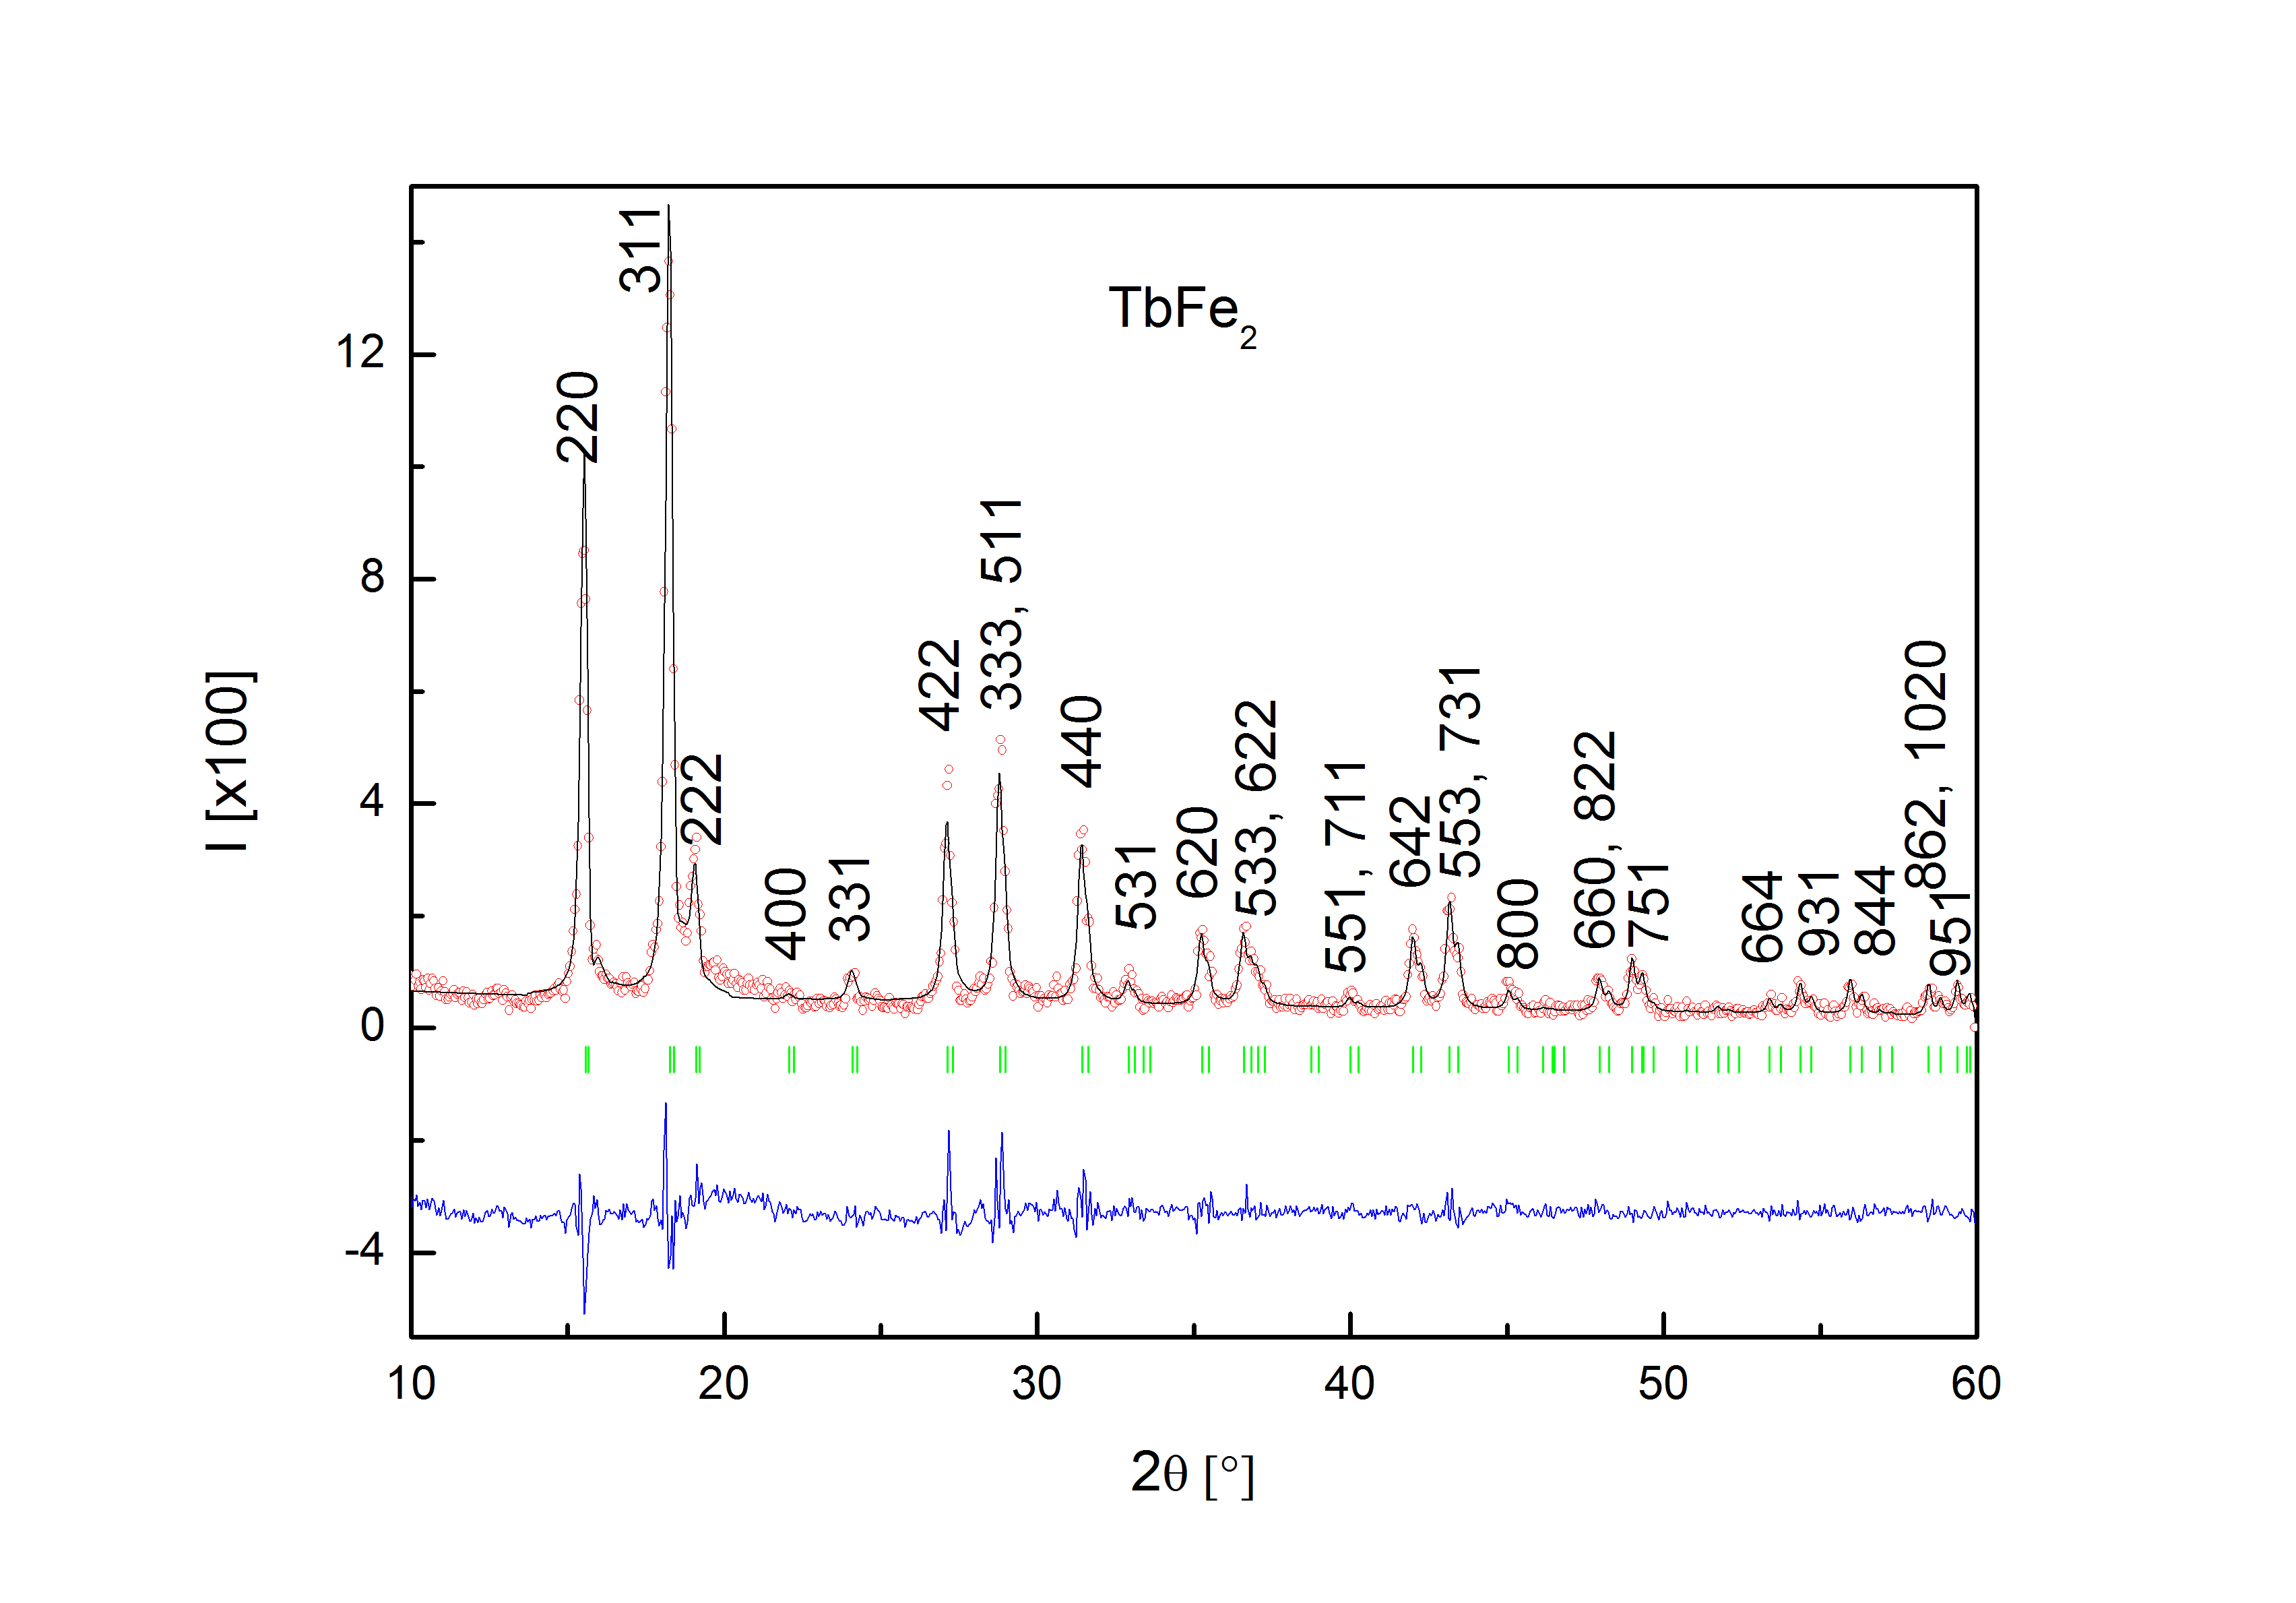
\includegraphics[width=0.85\linewidth]{../img/dif/TbFe2rentgen}
  \caption{Dyfraktogram rentgenowski próbki $\nit{Tb}\nit{Fe}_2$}
  \label{Tbrentgen}
\end{sidewaysfigure}

\newpage
\begin{sidewaysfigure}[htp]
  \centering
  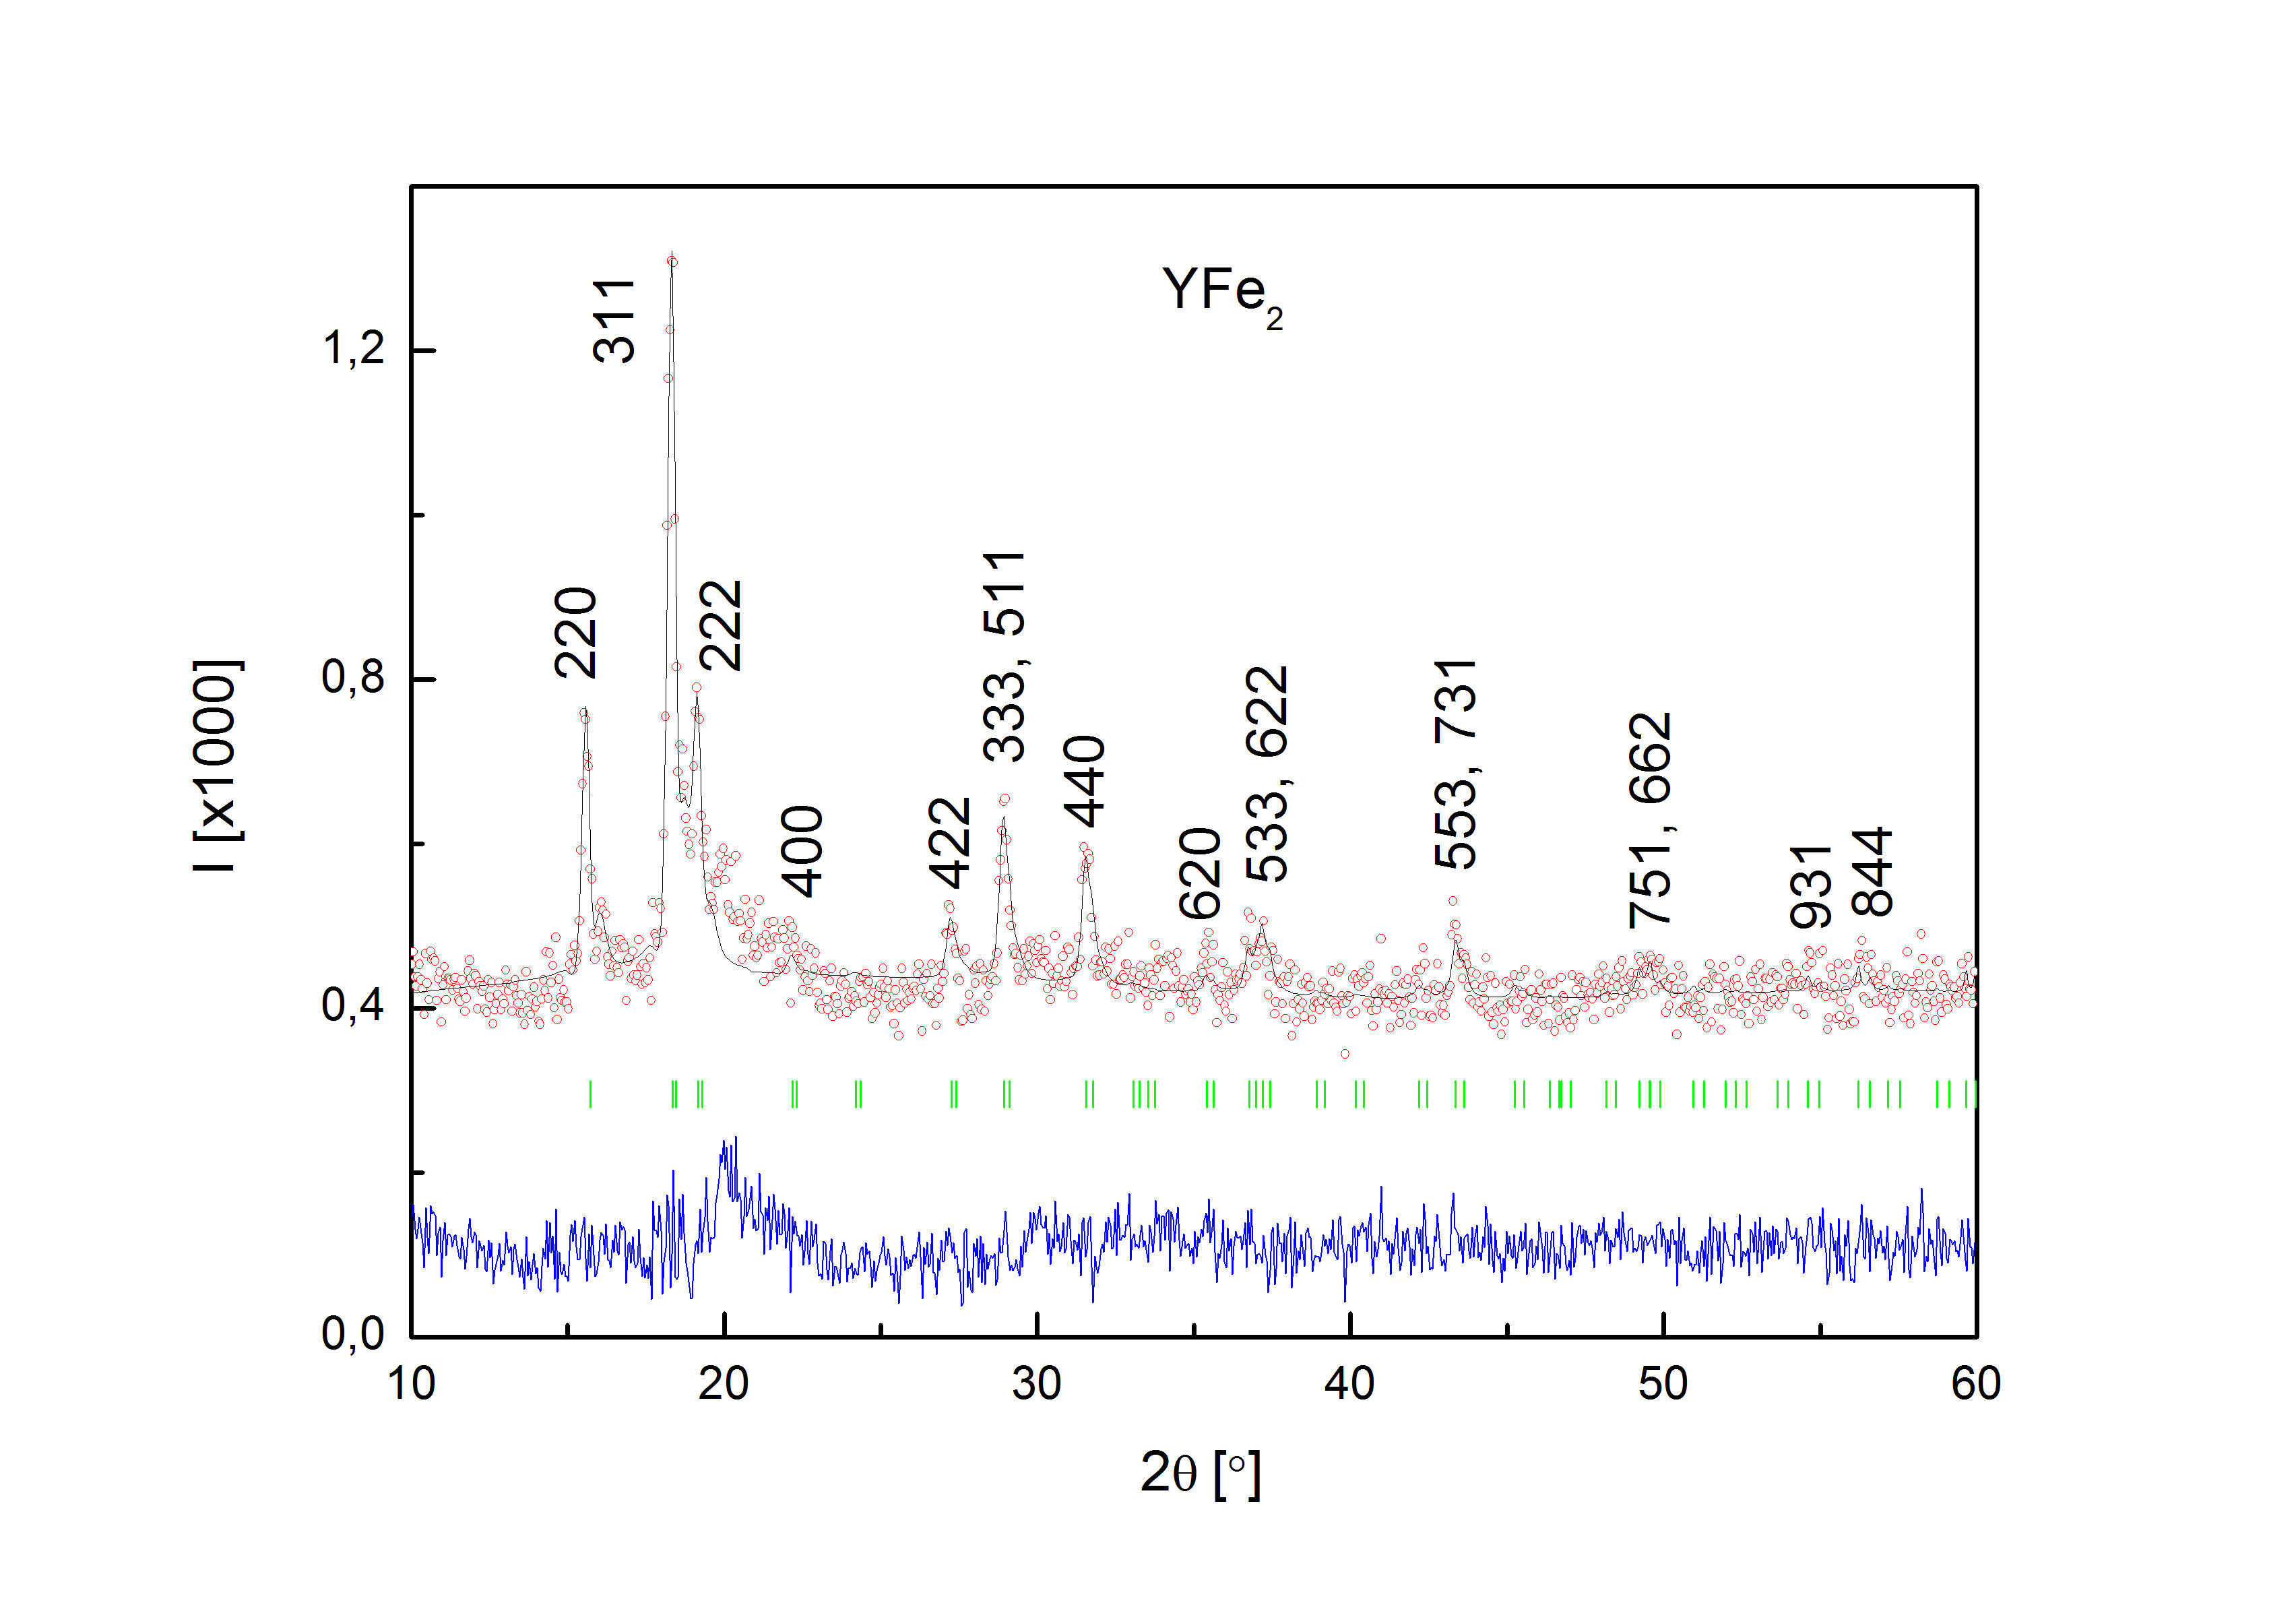
\includegraphics[width=0.85\linewidth]{../img/dif/YFe2rentgen}
  \caption{Dyfraktogram rentgenowski próbki $\nit{Y}\nit{Fe}_2$}
  \label{Yrentgen}
\end{sidewaysfigure}

\restoregeometry
\newgeometry{vmargin={2.5cm,2.5cm}, height=10.0in}

FullProf jako wynik analizy oprócz dopasowania podaje także wiele przydatnych parametrów. Z punktu widzenia tej pracy najciekawsze są stała sieci a oraz objętość komórki elementarnej V wraz z ich niepewnościami. Dane te zostały zebrane w tabeli \ref{parKomTab} 
oraz na wykresach \ref{aKomorki}-\ref{vKomorki}


\begin{table}[!ht]
  \centering
  \caption{Parametry komórek elementarnych wraz z niepewnościami}
  \label{parKomTab}
  \begin{tabular}{|c|c|c|c|}
    \hline
Związek	&	Zmierzone a $\AA$	&	Literaturowe a $\AA$	&	Zmierzone V $\AA^3$	\\\hline
$DyFe_2$	&	7,37557	&	7,36300	&	401,22370	\\\hline
$GdFe_2$	&	7,39786	&	7,37600	&	404,87256	\\\hline
$HoFe_2$	&	7,35860	&	7,34100	&	398,46043	\\\hline
$TbFe_2$	&	7,33366	&	7,30900	&	394,42387	\\\hline
$YFe_2$	&	7,31398	&	7,28700	&	391,25628	\\\hline

  \end{tabular}
\end{table}

Do wykresów dopasowano wielomiany drugiego stopnia, a dla parametru a sieci krystalicznej dodano również wartość tego parametru dla Terfenolu D dzięki uprzejmości pani dr Barbary Winiarskiej, oraz porównano je z wartościami literaturowymi zaczerpniętymi z TU JAKIŚ ODNOŚNIK DO LITERATURY.

\begin{figure}[h]
    \centering
    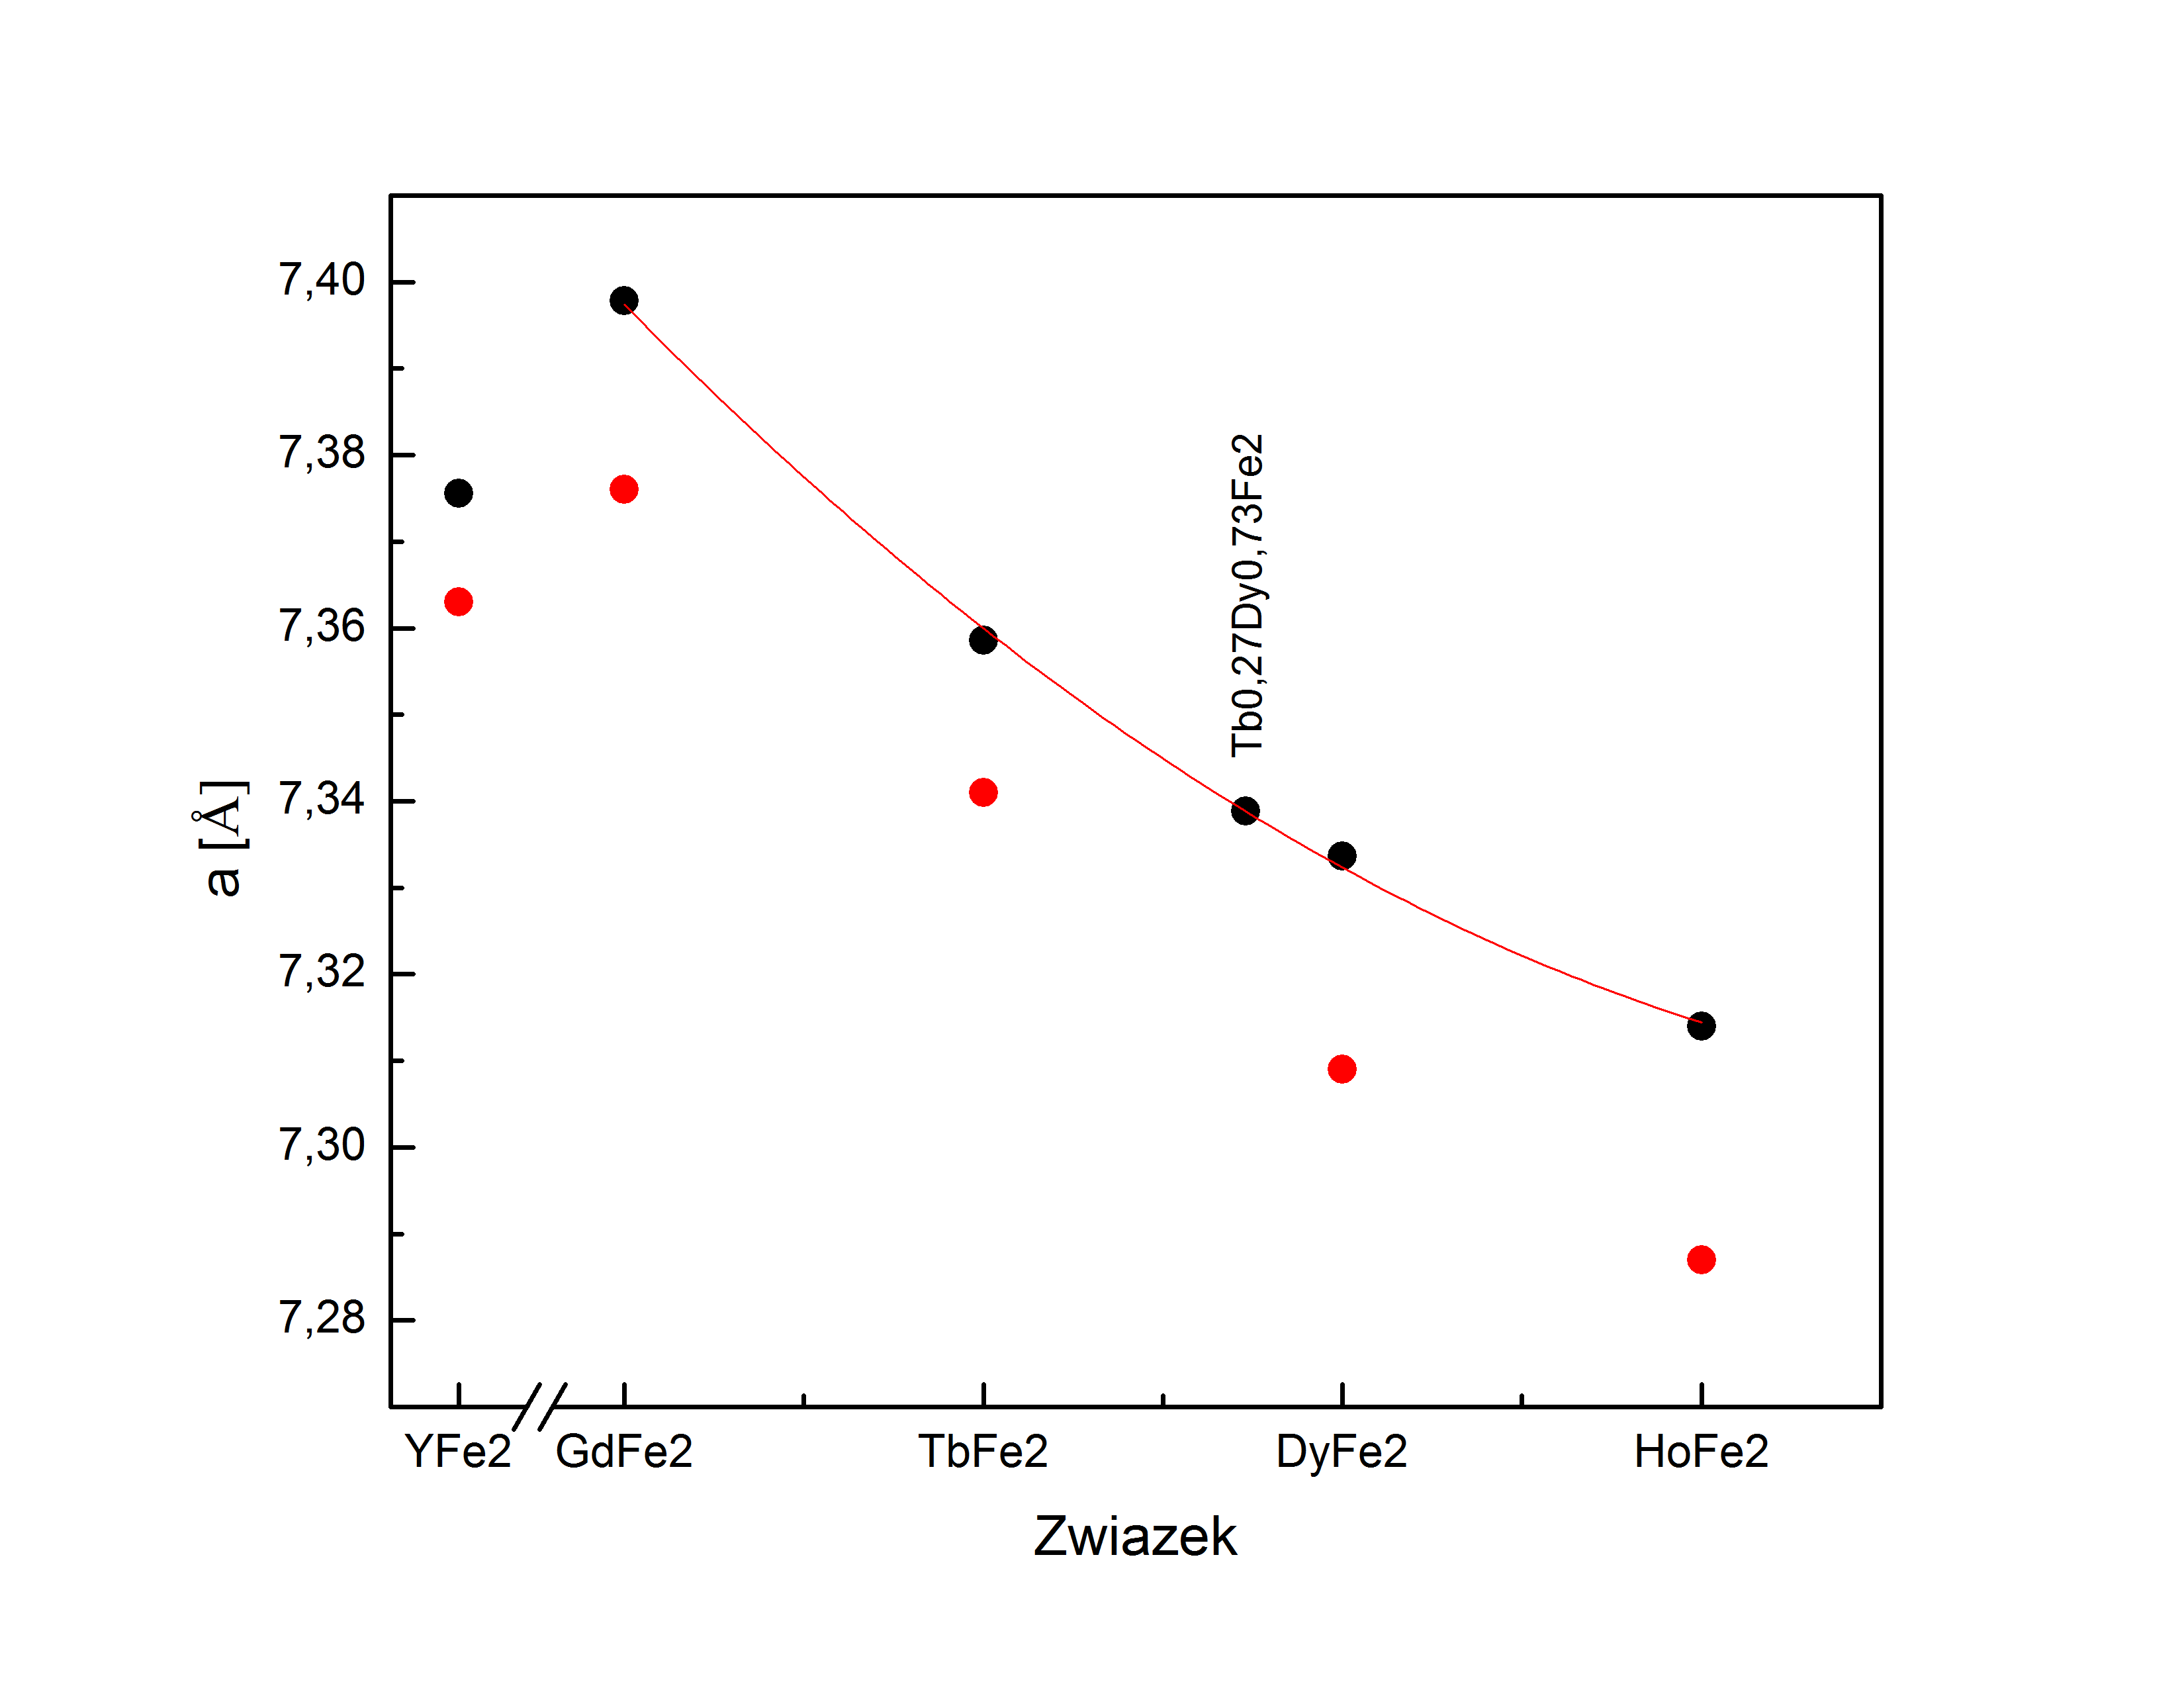
\includegraphics[width =0.9\textwidth]{../img/aKomorki}
    \caption{Wartości parametru a sieci krystalicznej badanych próbek}
    \label{aKomorki}
\end{figure}

\begin{figure}[h]
    \centering
    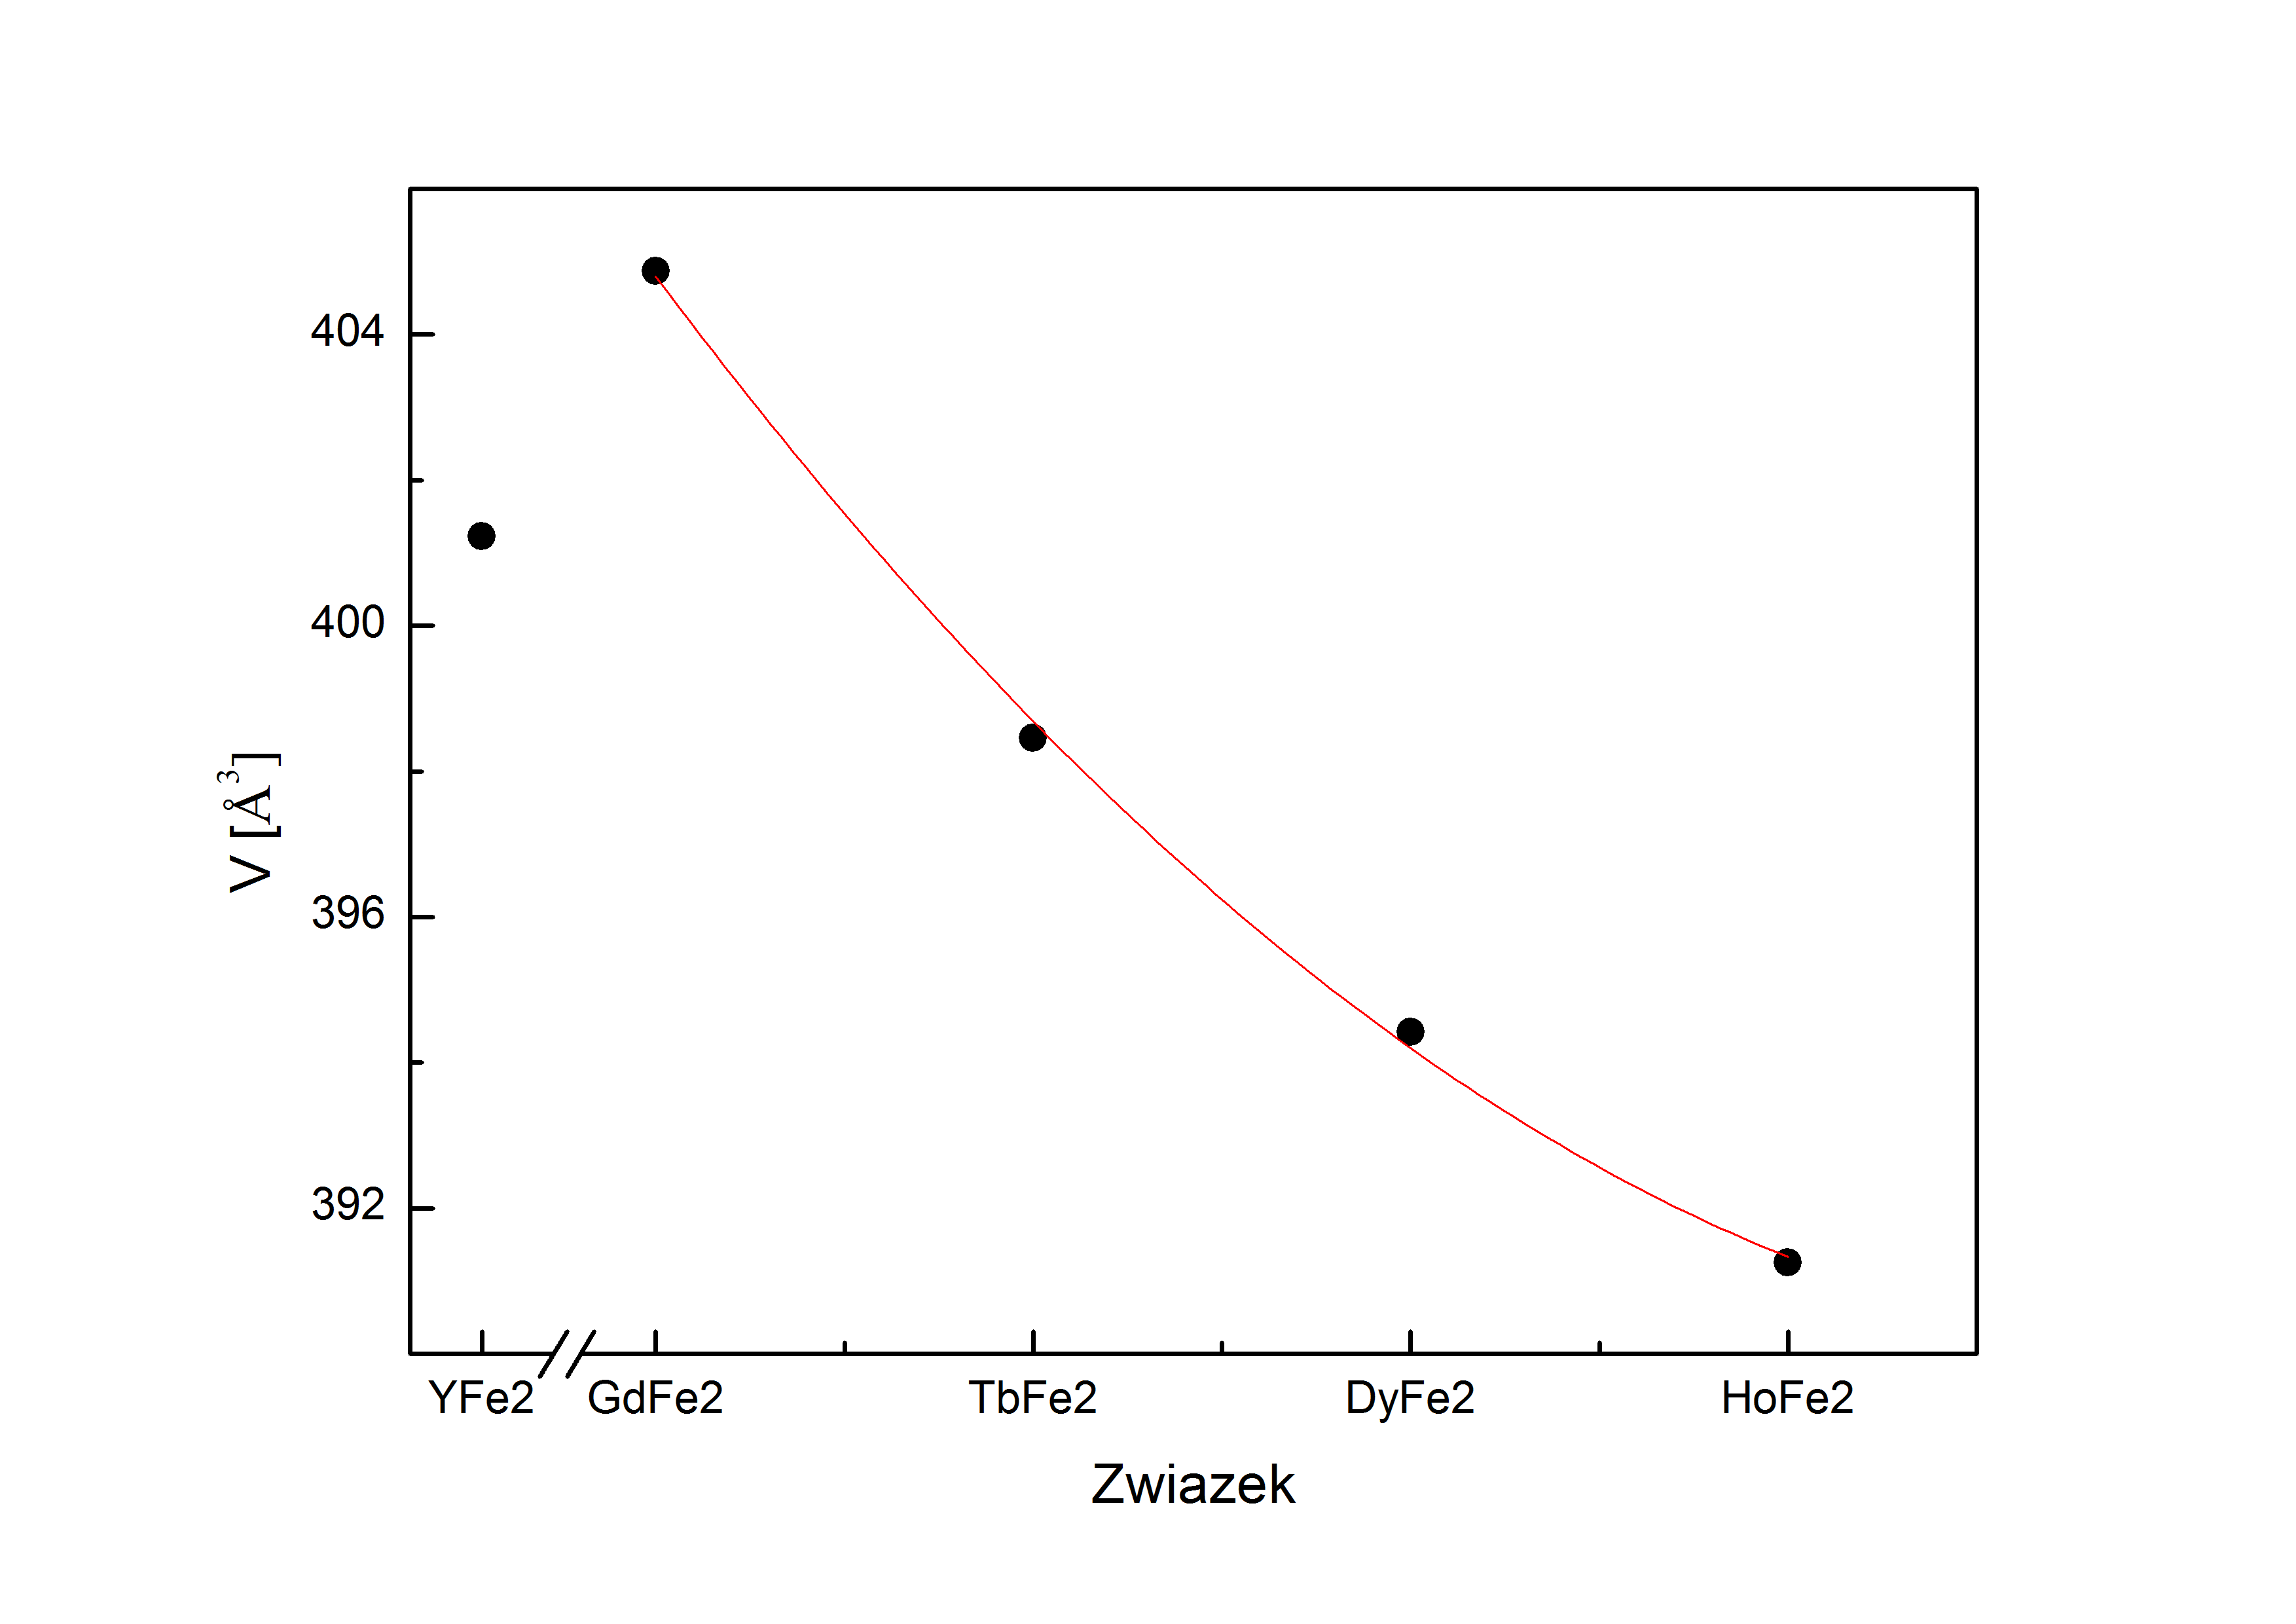
\includegraphics[width =0.9\textwidth]{../img/vKomorki}
    \caption{Wartości objętości V badanych próbek}
    \label{vKomorki}
\end{figure}

Jak wynika z wykresu \ref{aKomorki} otrzymane wartości parametru sieci krystalicznej a są wyższe od wartości literaturowych. Zaobserwowane zjawisko kontrakcji oraz zgodność wartości dla Terfenolu D wykonanego na tej samej aparaturze świadczą o tym, że badanie zostało przeprowadzone poprawnie, a powstała różnica między wartościami wynika nie z błędu wykonującego, lecz jest spoodoana czynnikami temparaturowymi 


\newpage
%-------------------------------------------------------------------------------------
%------------------------------wyniki magnetostrykcji----------------------------
%-------------------------------------------------------------------------------------
\subsection{Wyniki pomiarów magnetostrykcji}

Poniższe rysunki \ref{Dypoprzeczna} - \ref{YObjetosc} przedstawiają wyniki pomiarów magnetostrykcji wzdłużnej
 $\lambda_{\parallel}$ i poprzecznej $\lambda_{\perp}$, 
oraz wyliczone za ich pomocą według wzorów \ref{lambdaksztaltu} i \ref{lambdaobjetosci} wartości magnetostrykcji kształtu $\lambda_{\tau}$  i objętości $\lambda_{V}$.
 \begin{equation}
    \lambda_{\tau}=\lambda_{\parallel} - \lambda_{\perp}
    \label{lambdaksztaltu}
  \end{equation}

  \begin{equation}
    \lambda_{\tau}=\lambda_{\parallel} + 2\lambda_{\perp}
    \label{lambdaobjetosci}
  \end{equation}

%---------------------------------------Dy-------------------------------------
 


\begin{figure}[h]
    \centering
    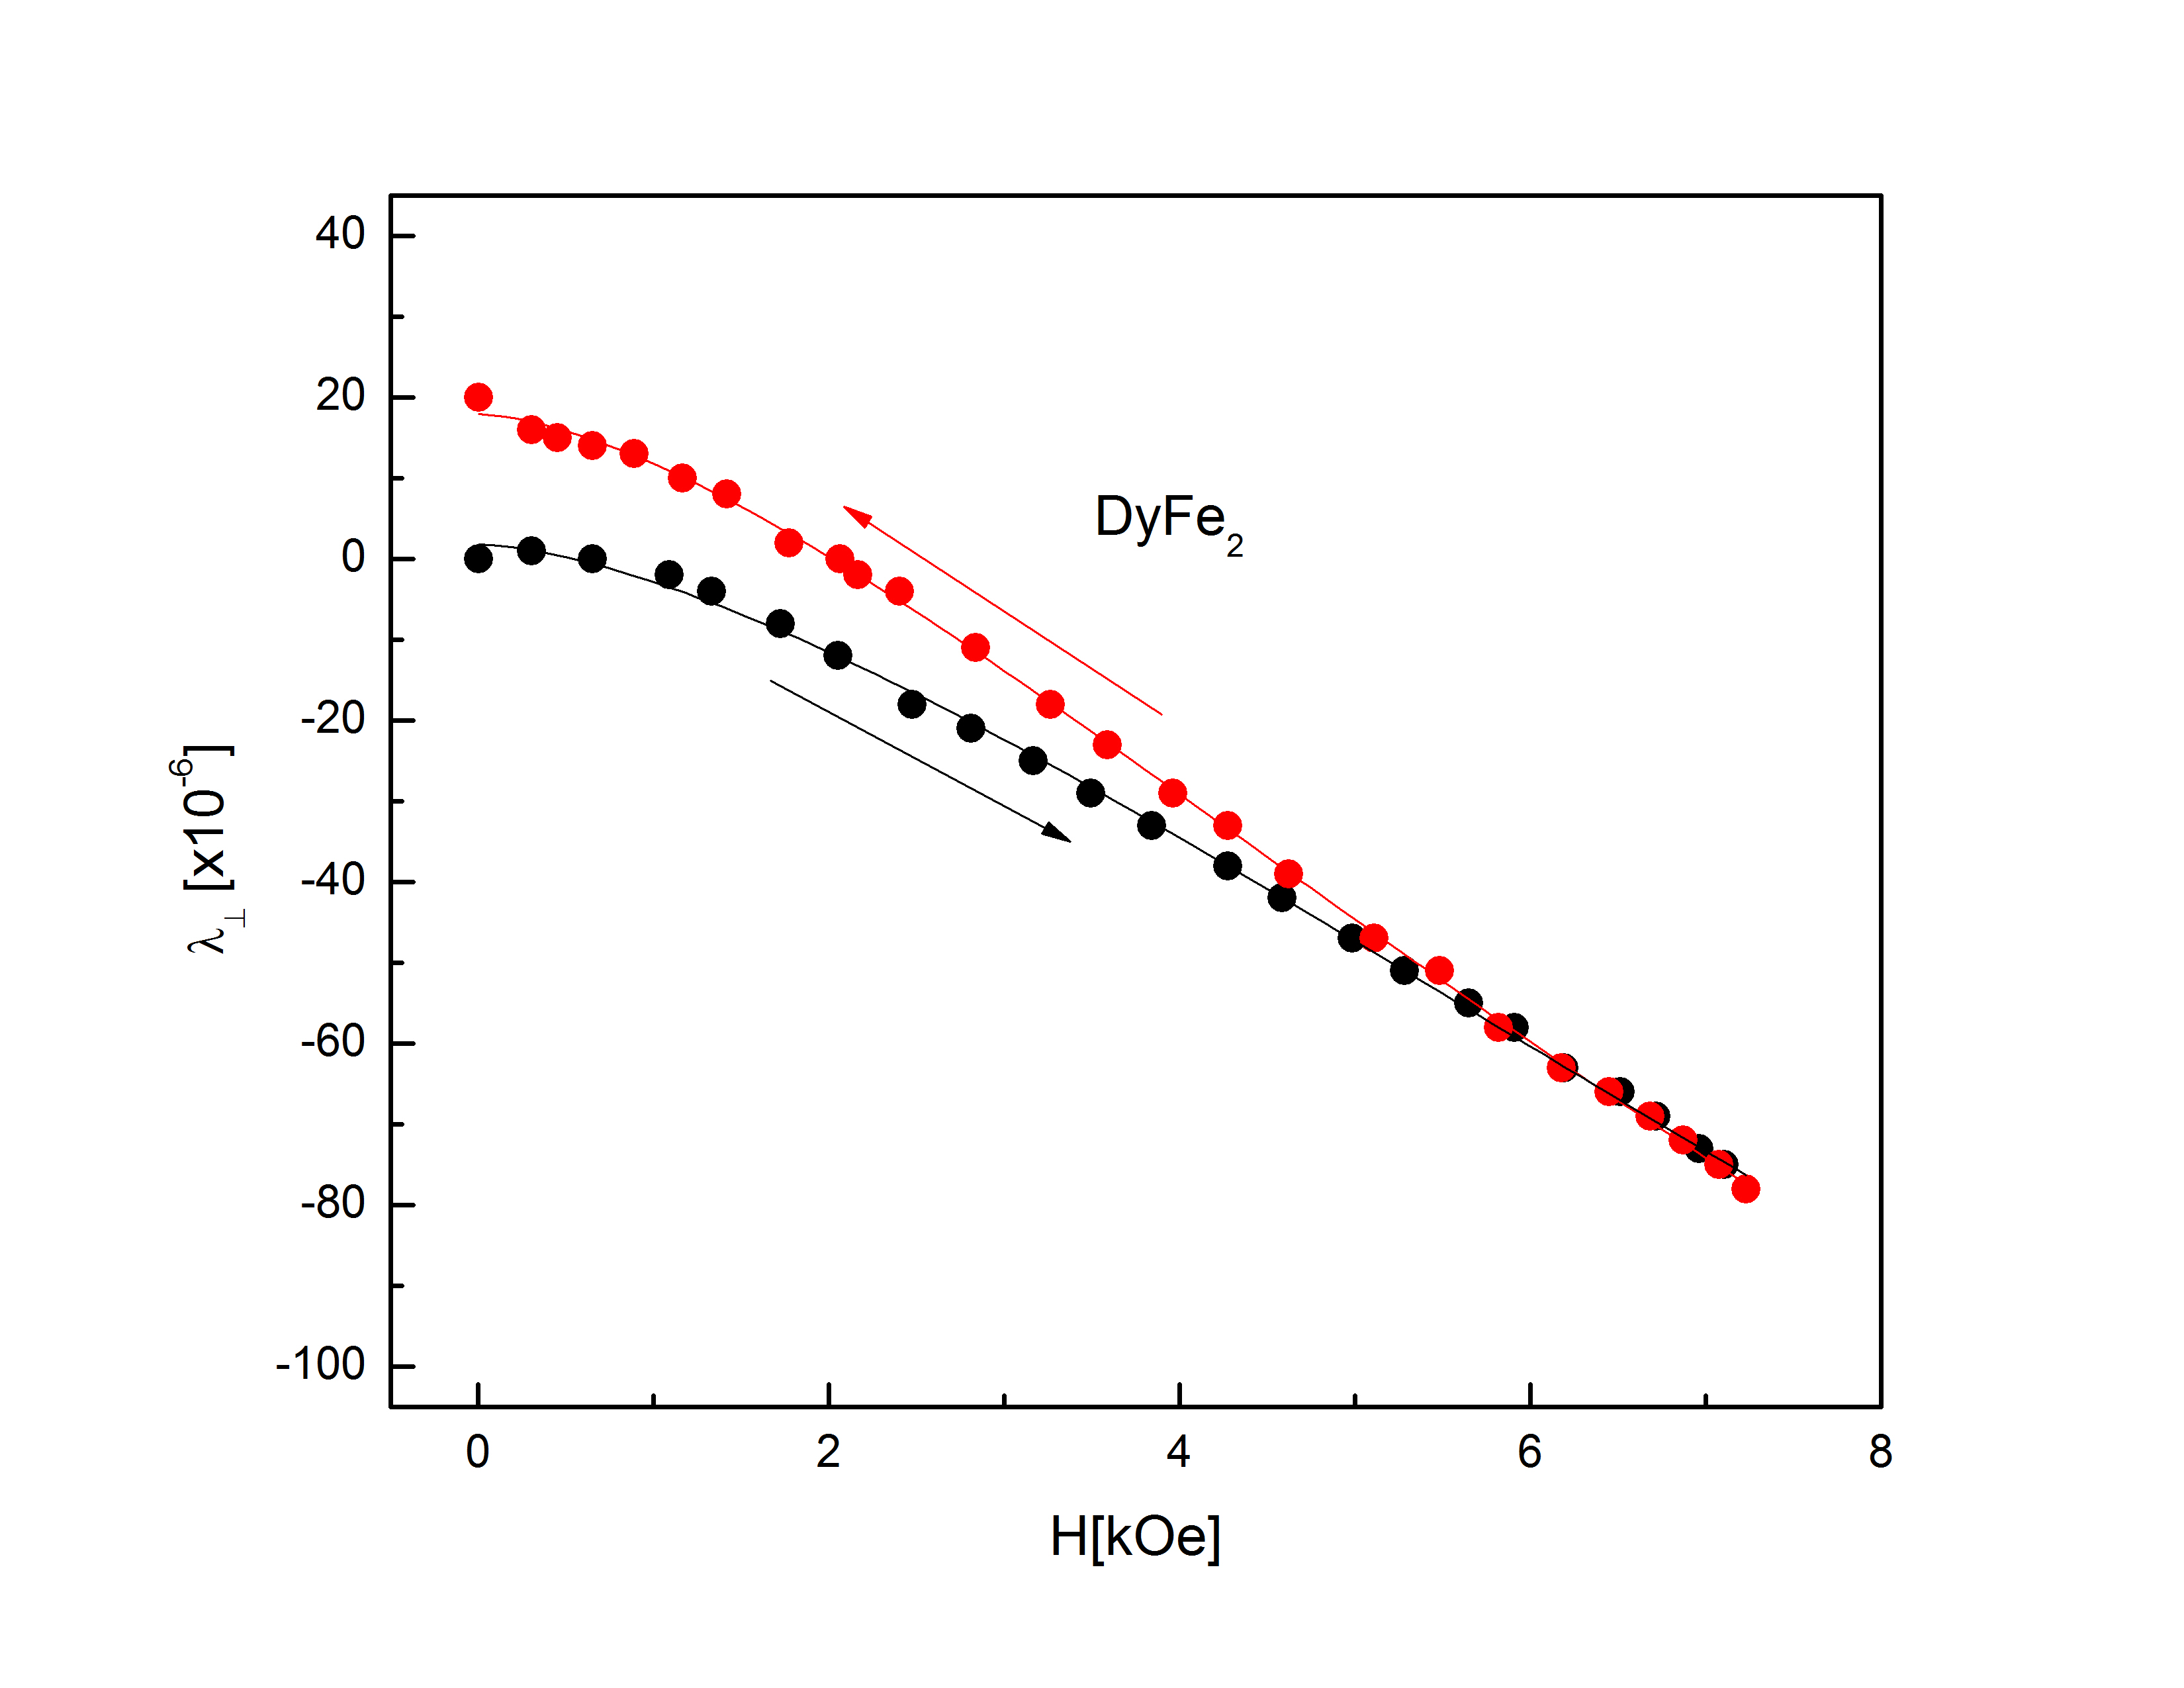
\includegraphics[width =0.9\textwidth]{../img/magneto/Dypoprzeczna}
    \caption{Wartość magnetostrykcji poprzecznej $\lambda_{\perp}$ $DyFe_2$}
    \label{Dypoprzeczna}
\end{figure}

\begin{figure}[h]
    \centering
    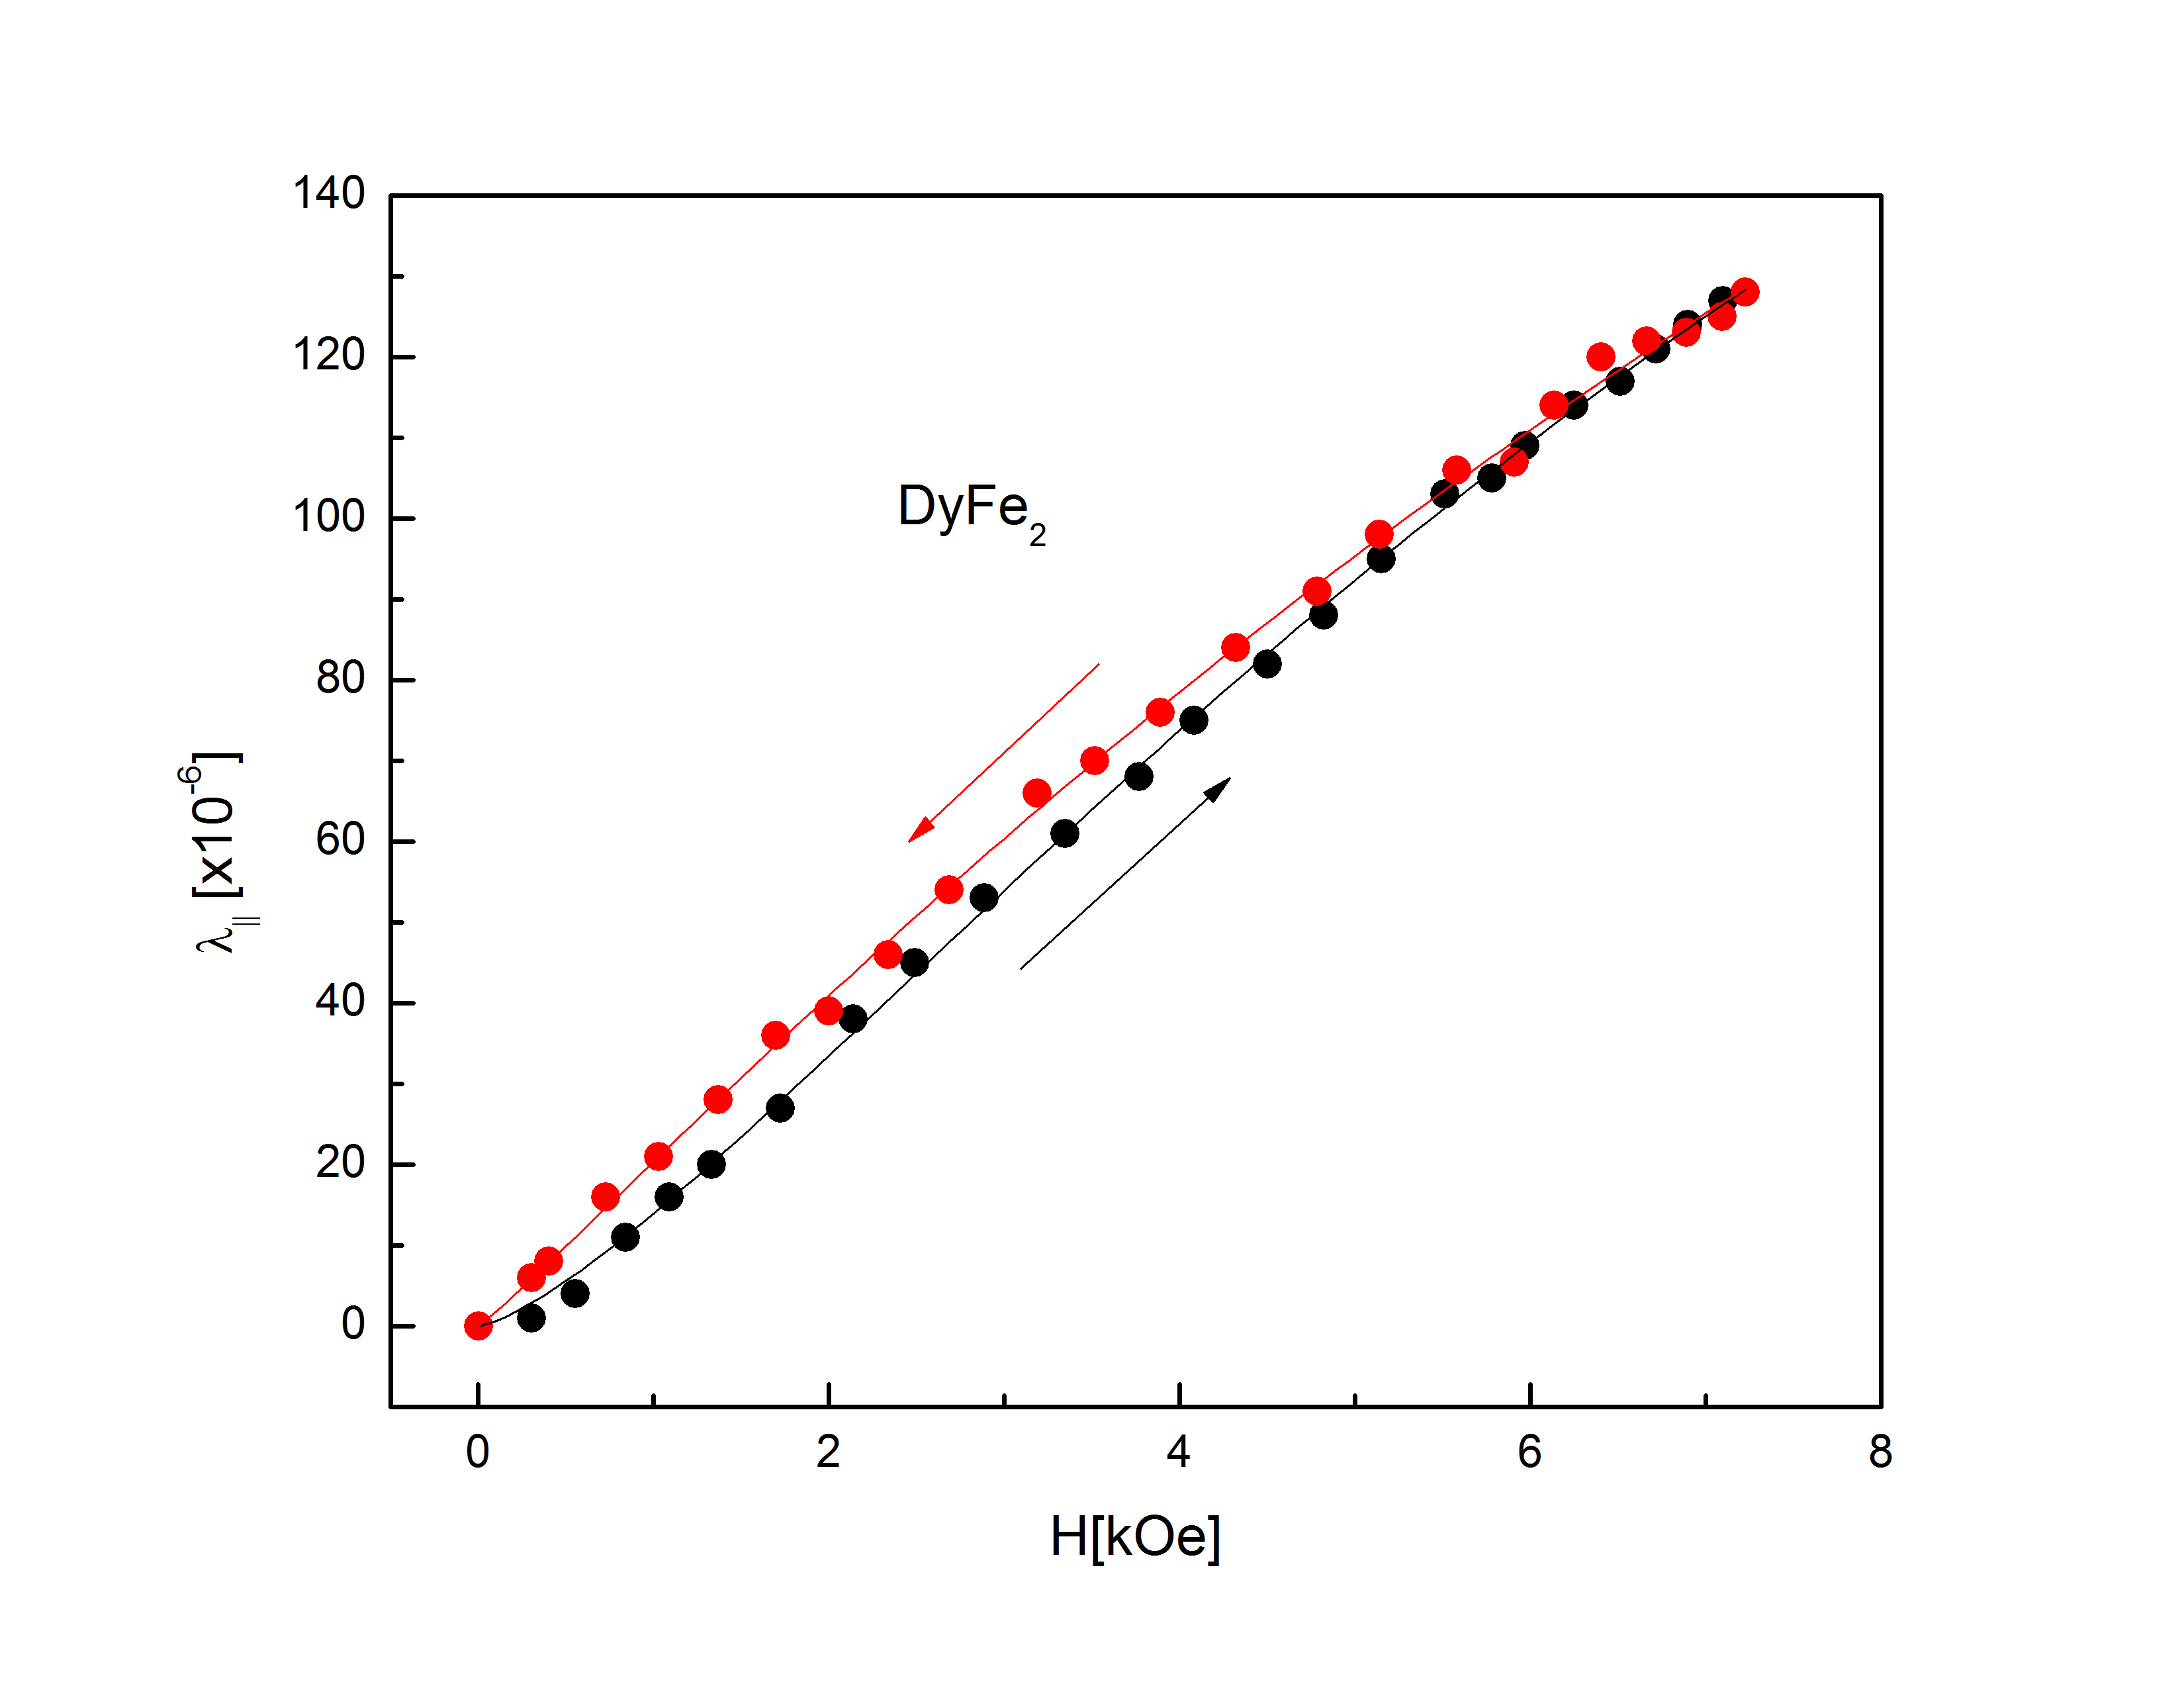
\includegraphics[width =0.9\textwidth]{../img/magneto/Dywzdluzna}
    \caption{Wartość magnetostrykcji wzdłużnej $\lambda_{\parallel}$ $DyFe_2$}
    \label{Dywzdluzna}
\end{figure}

\begin{figure}[h]
    \centering
    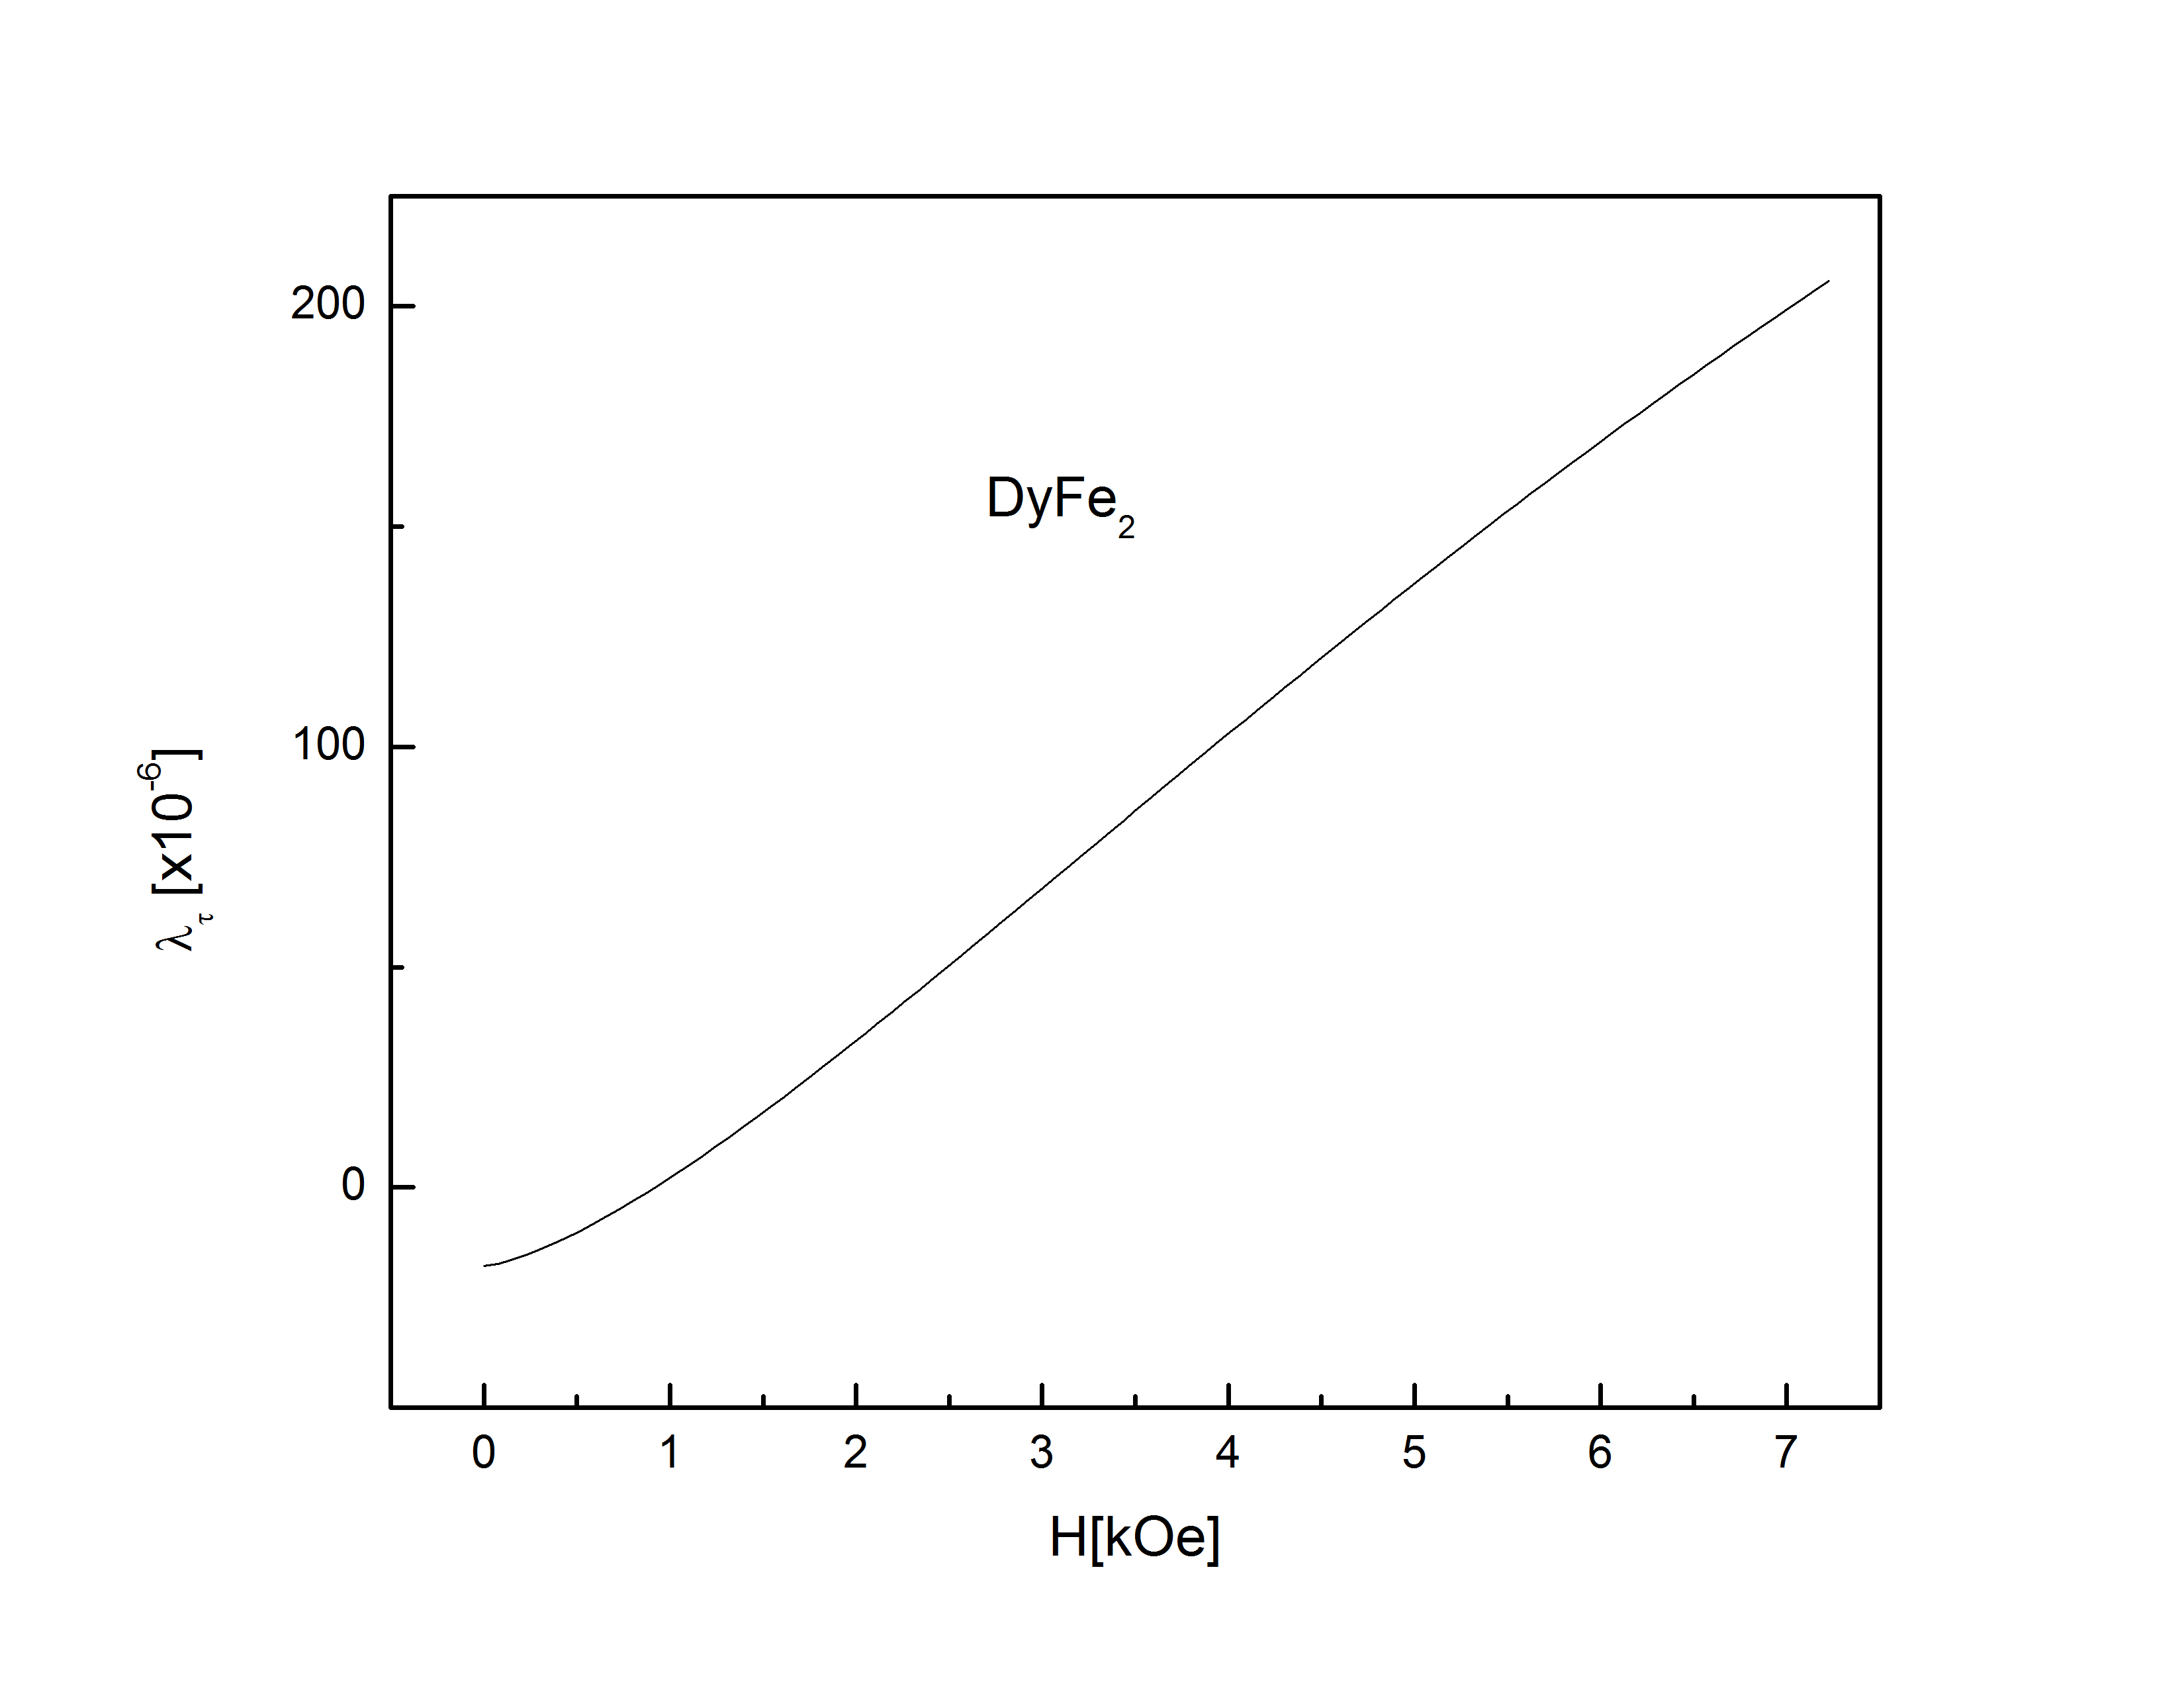
\includegraphics[width =0.9\textwidth]{../img/magneto/DyKsztaltu}
    \caption{Wartość magnetostrykcji kształru $\lambda_{\tau}$ $DyFe_2$}
    \label{DyKsztaltu}
\end{figure}

\begin{figure}[h]
    \centering
    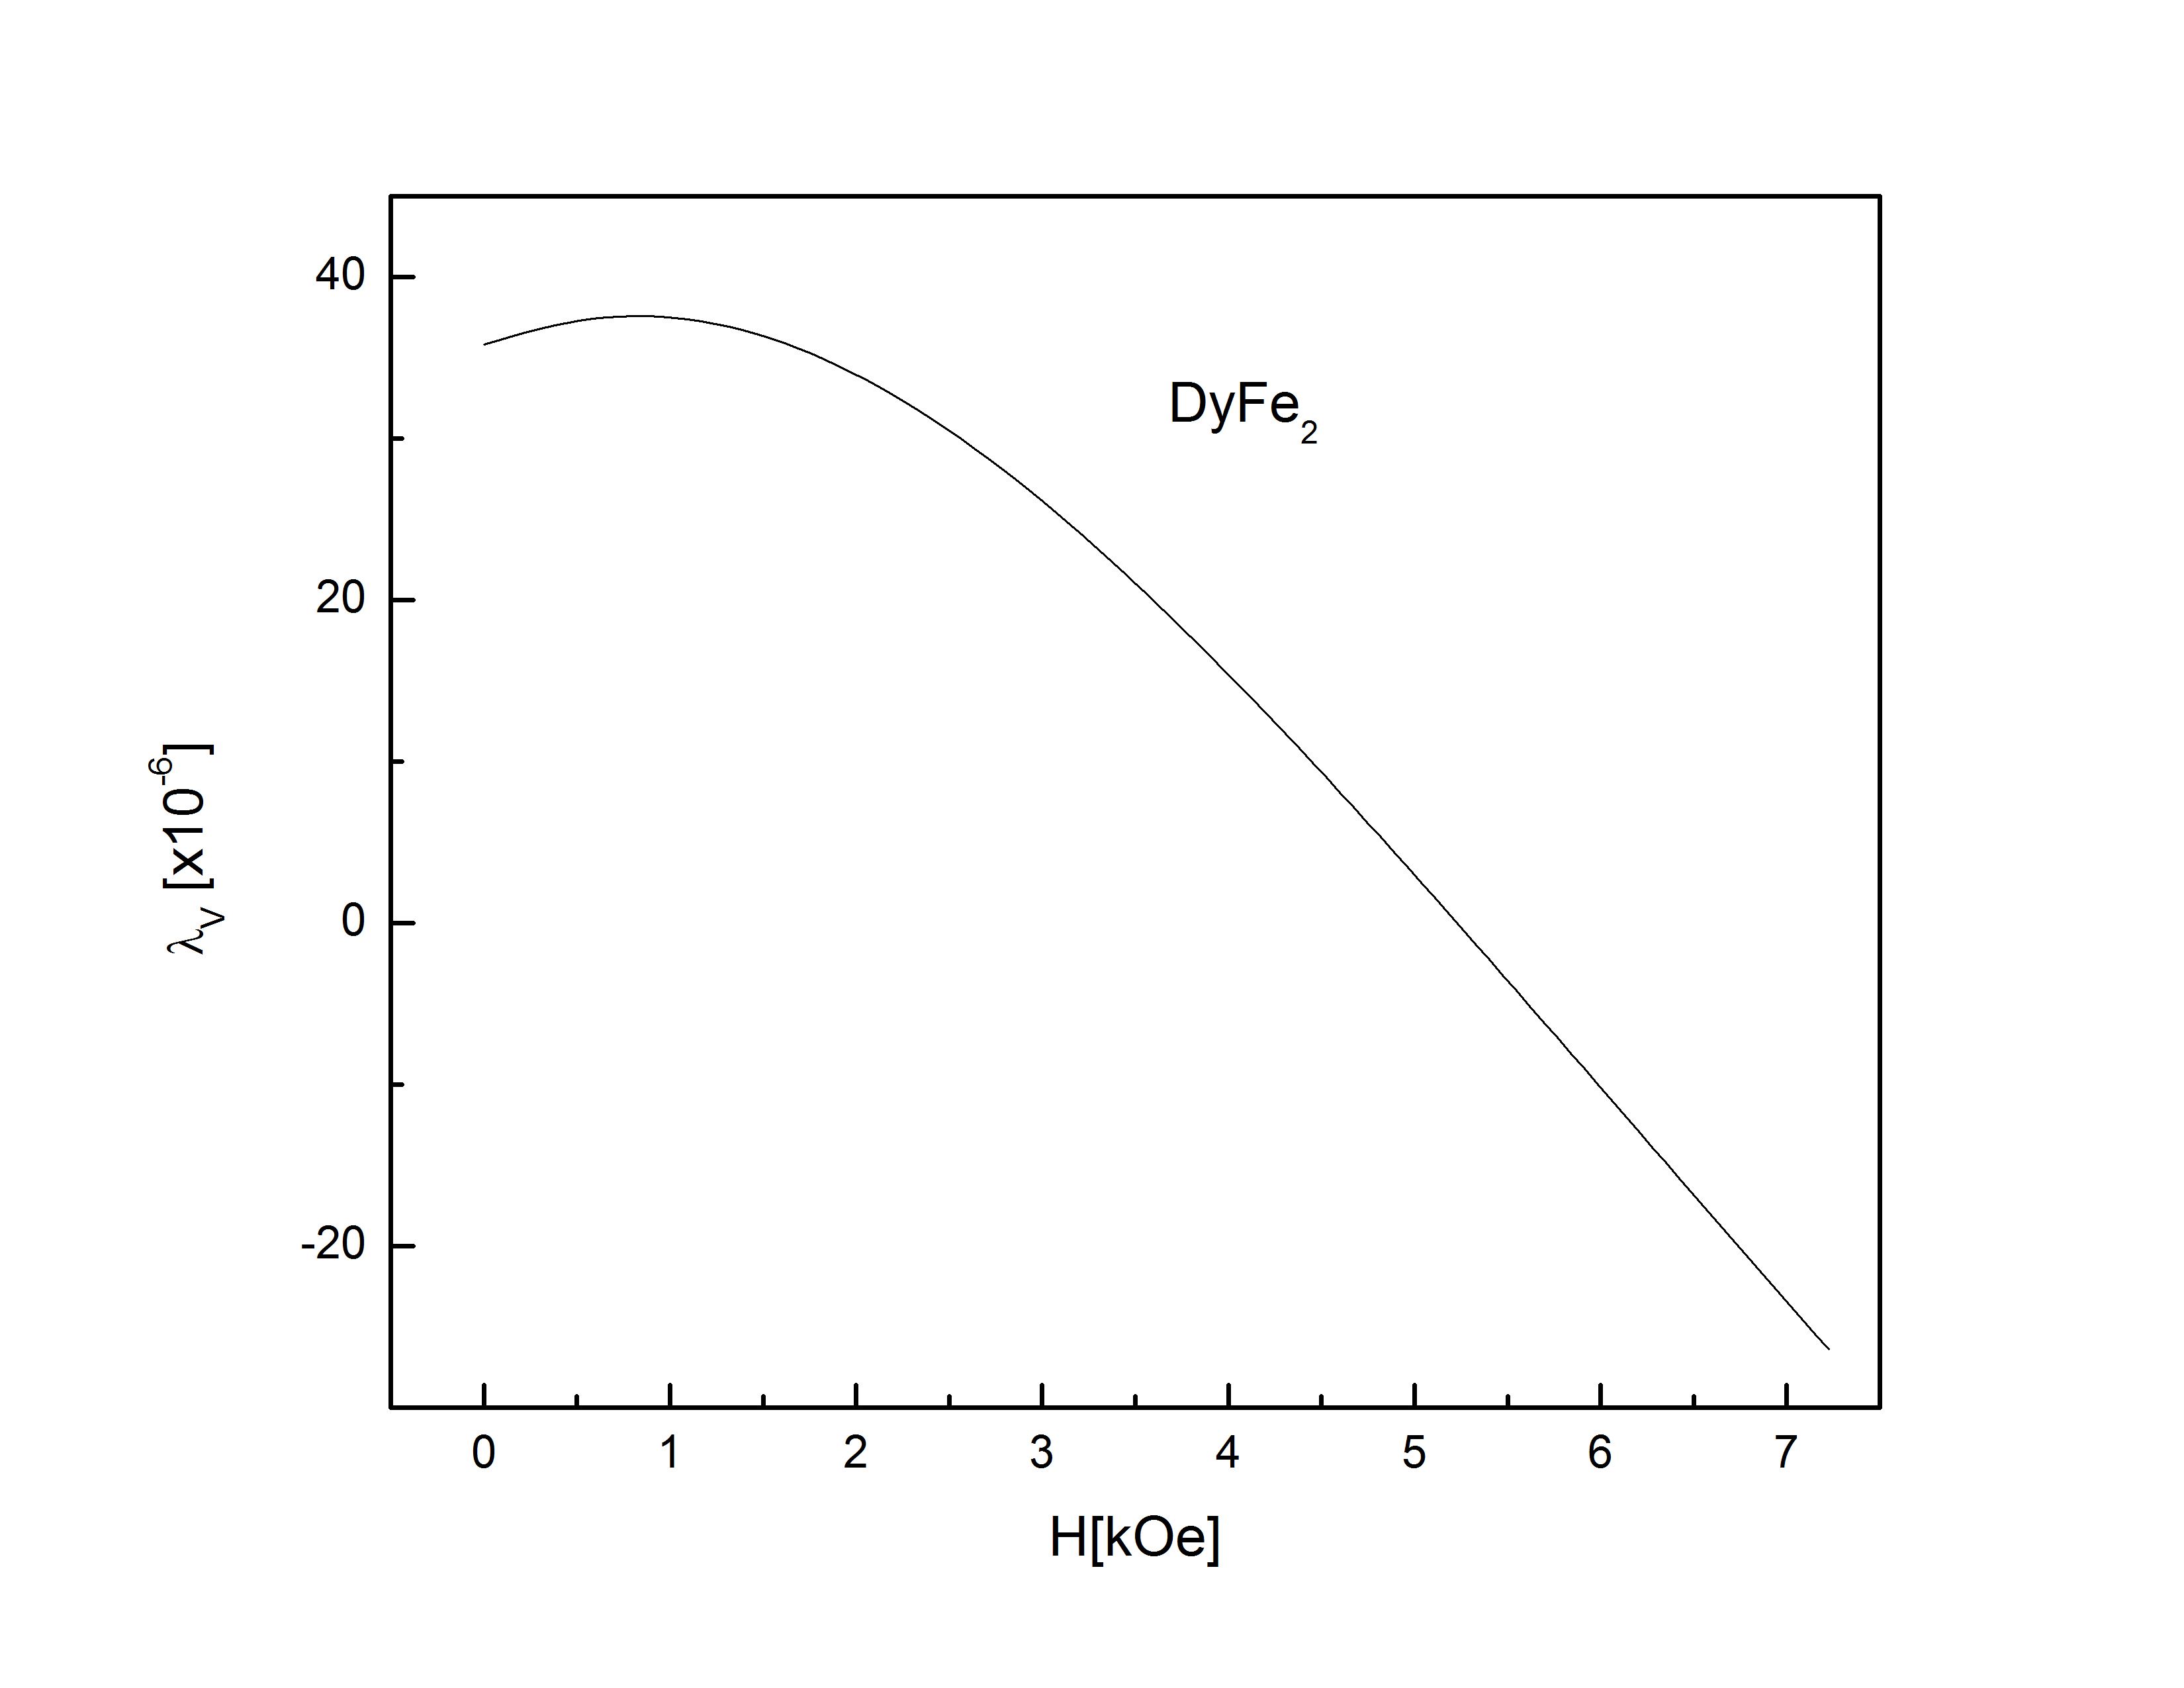
\includegraphics[width =0.9\textwidth]{../img/magneto/DyObjetosc}
    \caption{Wartość magnetostrykcji objetości $\lambda_{V}$ $DyFe_2$}
    \label{DyObjetosc}
\end{figure}


%---------------------------------------Gd-------------------------------------



\begin{figure}[h]
    \centering
    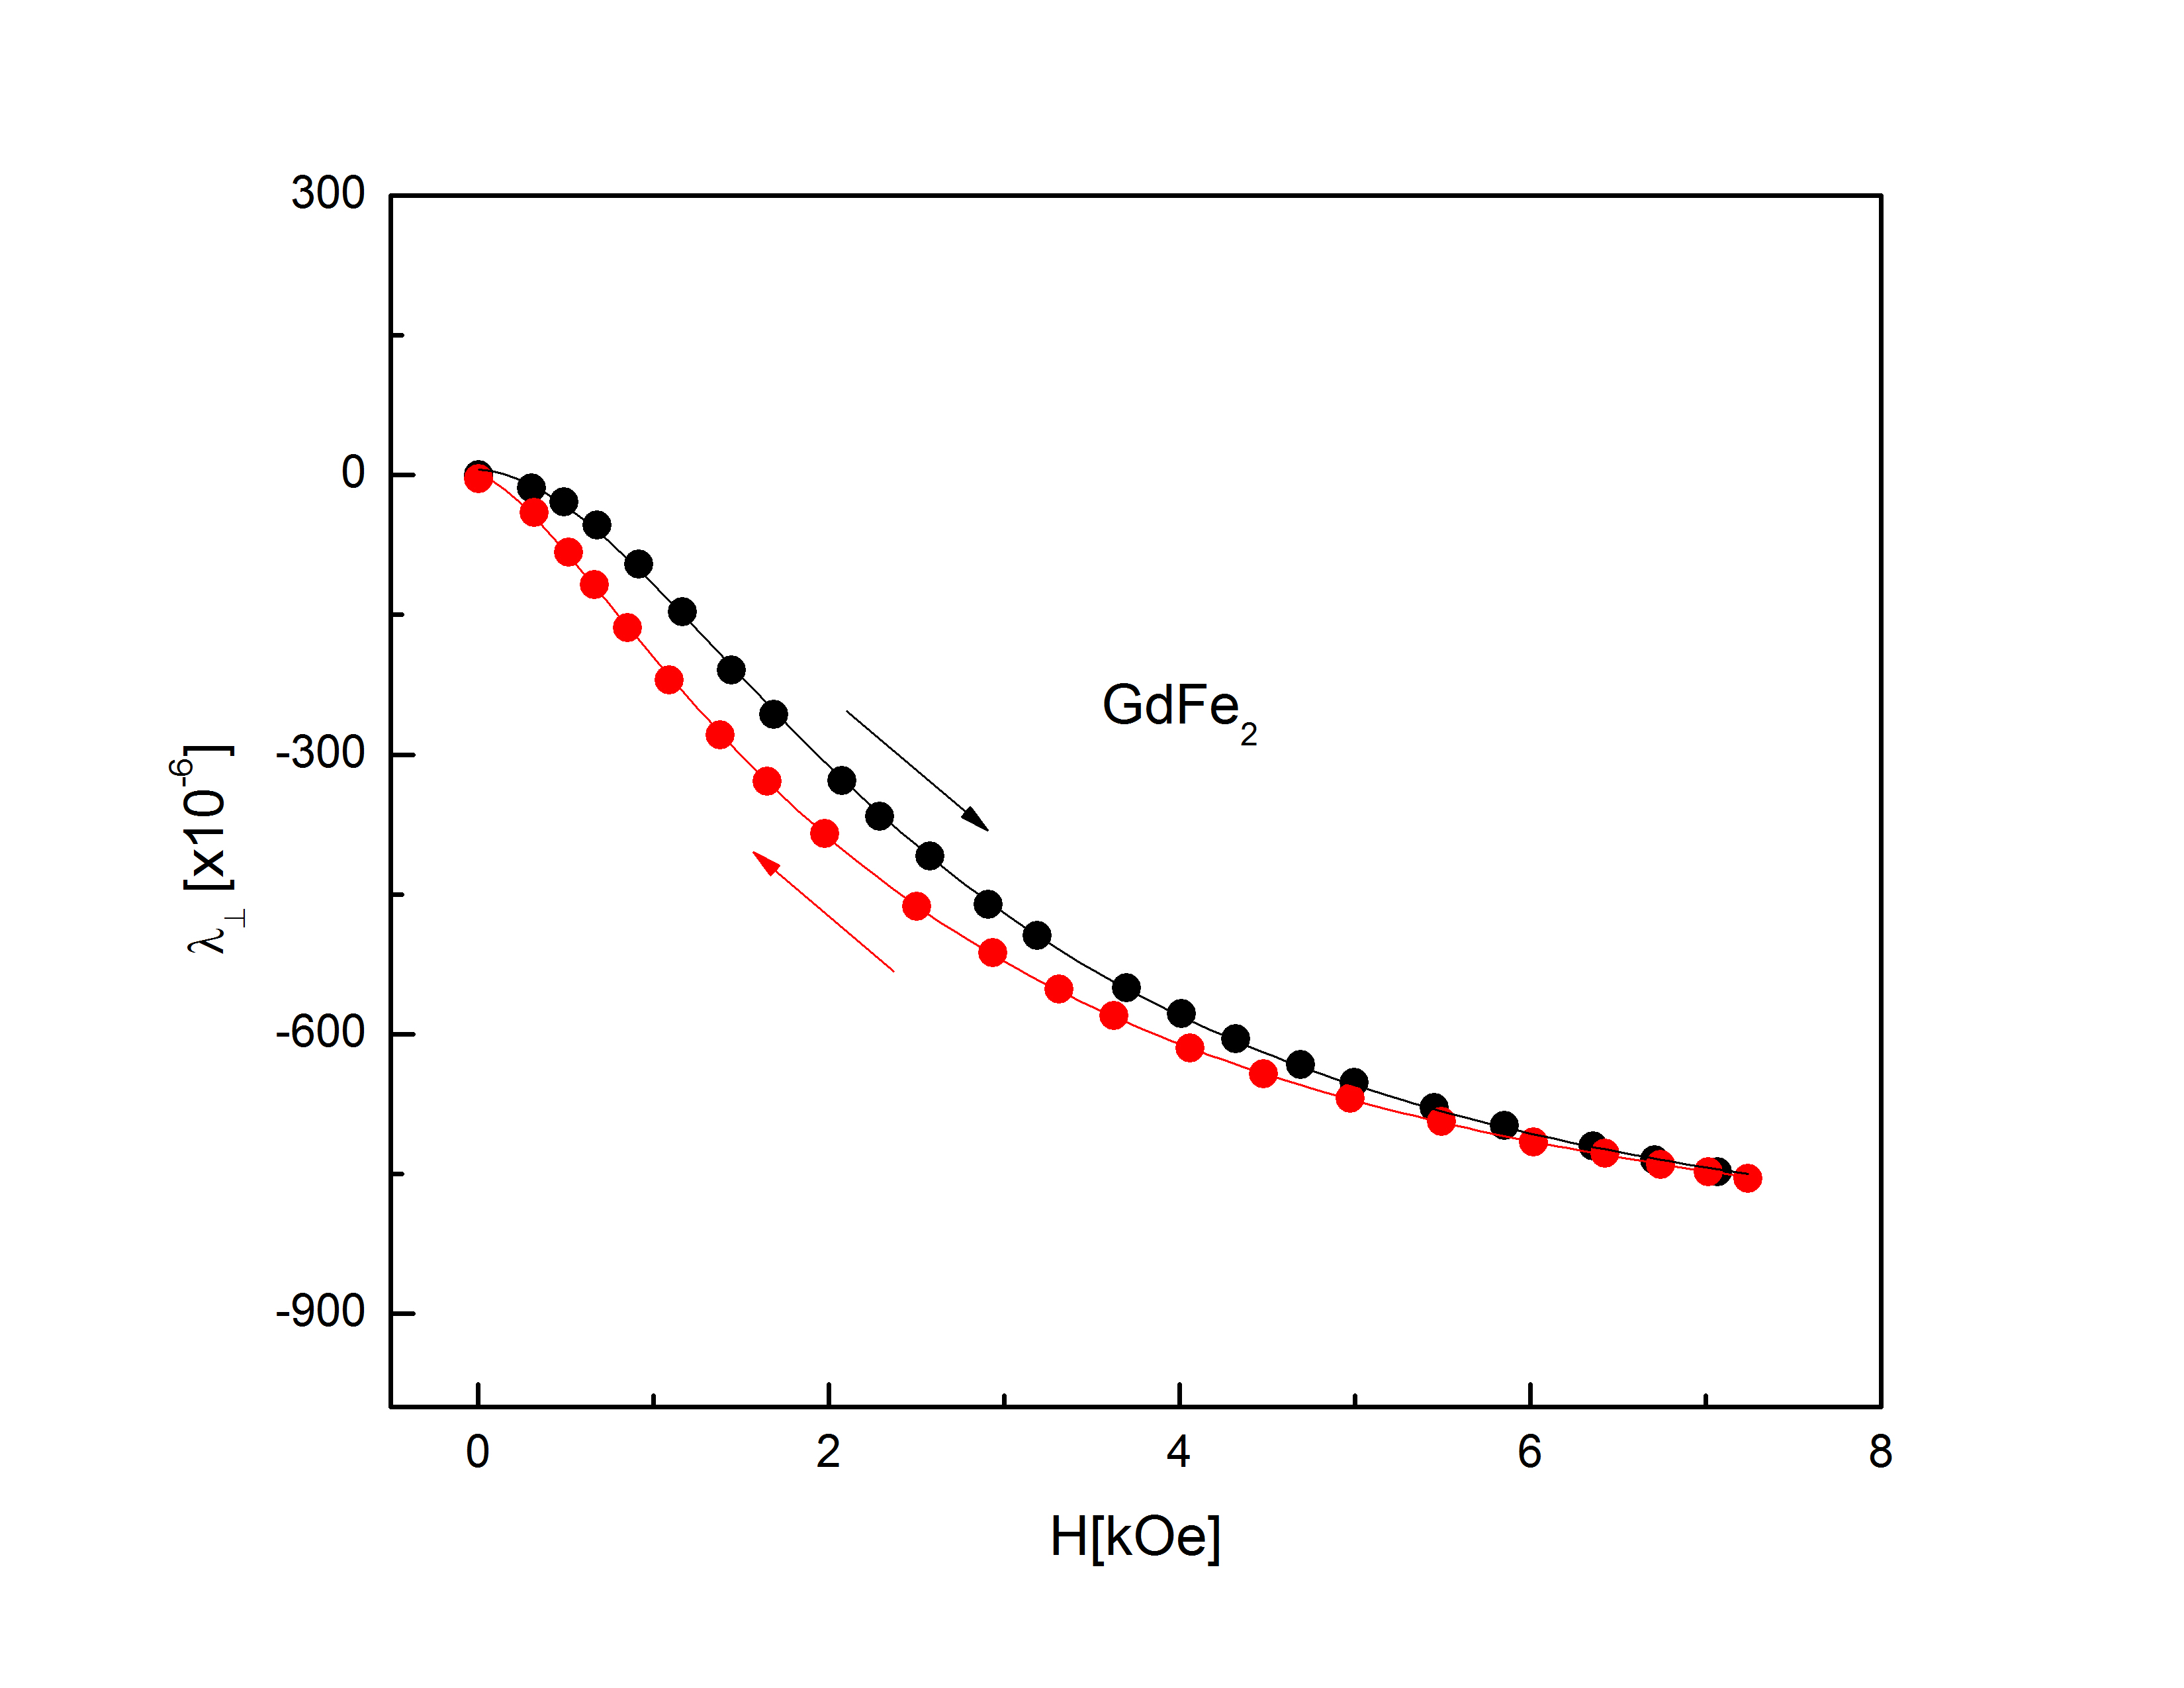
\includegraphics[width =0.9\textwidth]{../img/magneto/Gdpoprzeczna}
    \caption{Wartość magnetostrykcji poprzecznej $\lambda_{\perp}$ $GdFe_2$}
    \label{Gdpoprzeczna}
\end{figure}

\begin{figure}[h]
    \centering
    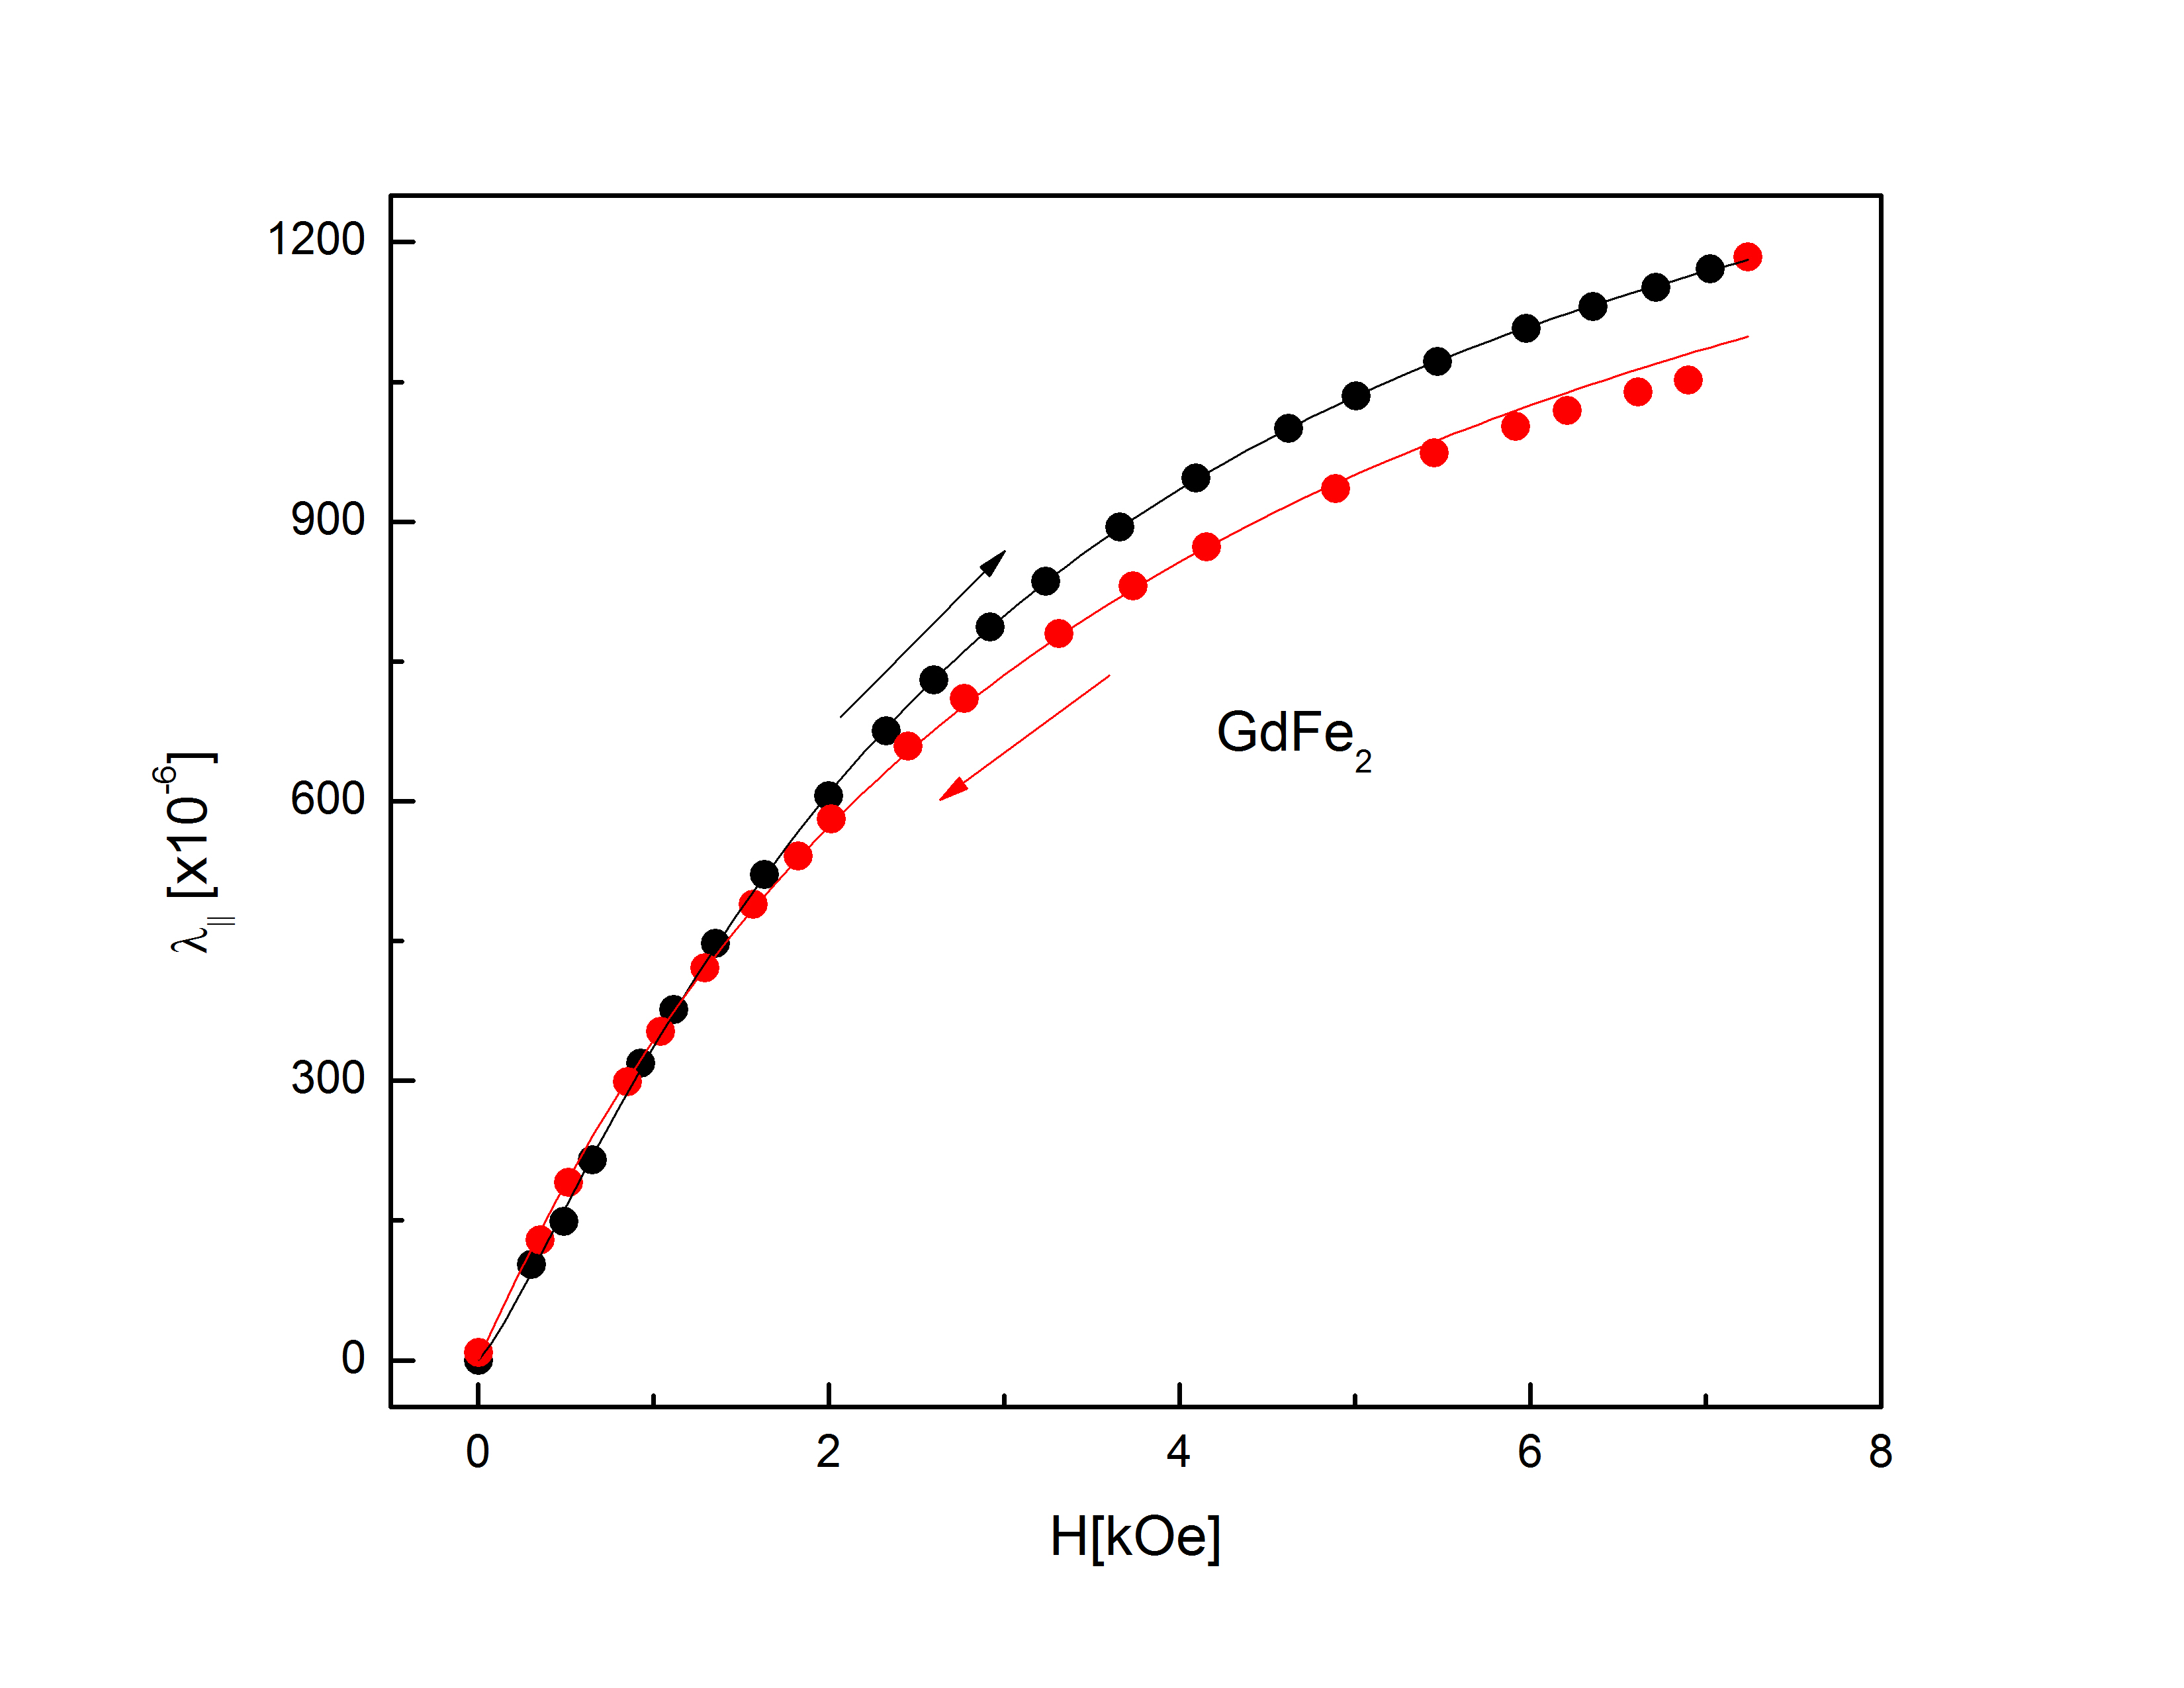
\includegraphics[width =0.9\textwidth]{../img/magneto/Gdwzdluzna}
    \caption{Wartość magnetostrykcji wzdłużnej $\lambda_{\parallel}$ $GdFe_2$}
    \label{Gdwzdluzna}
\end{figure}

\begin{figure}[h]
    \centering
    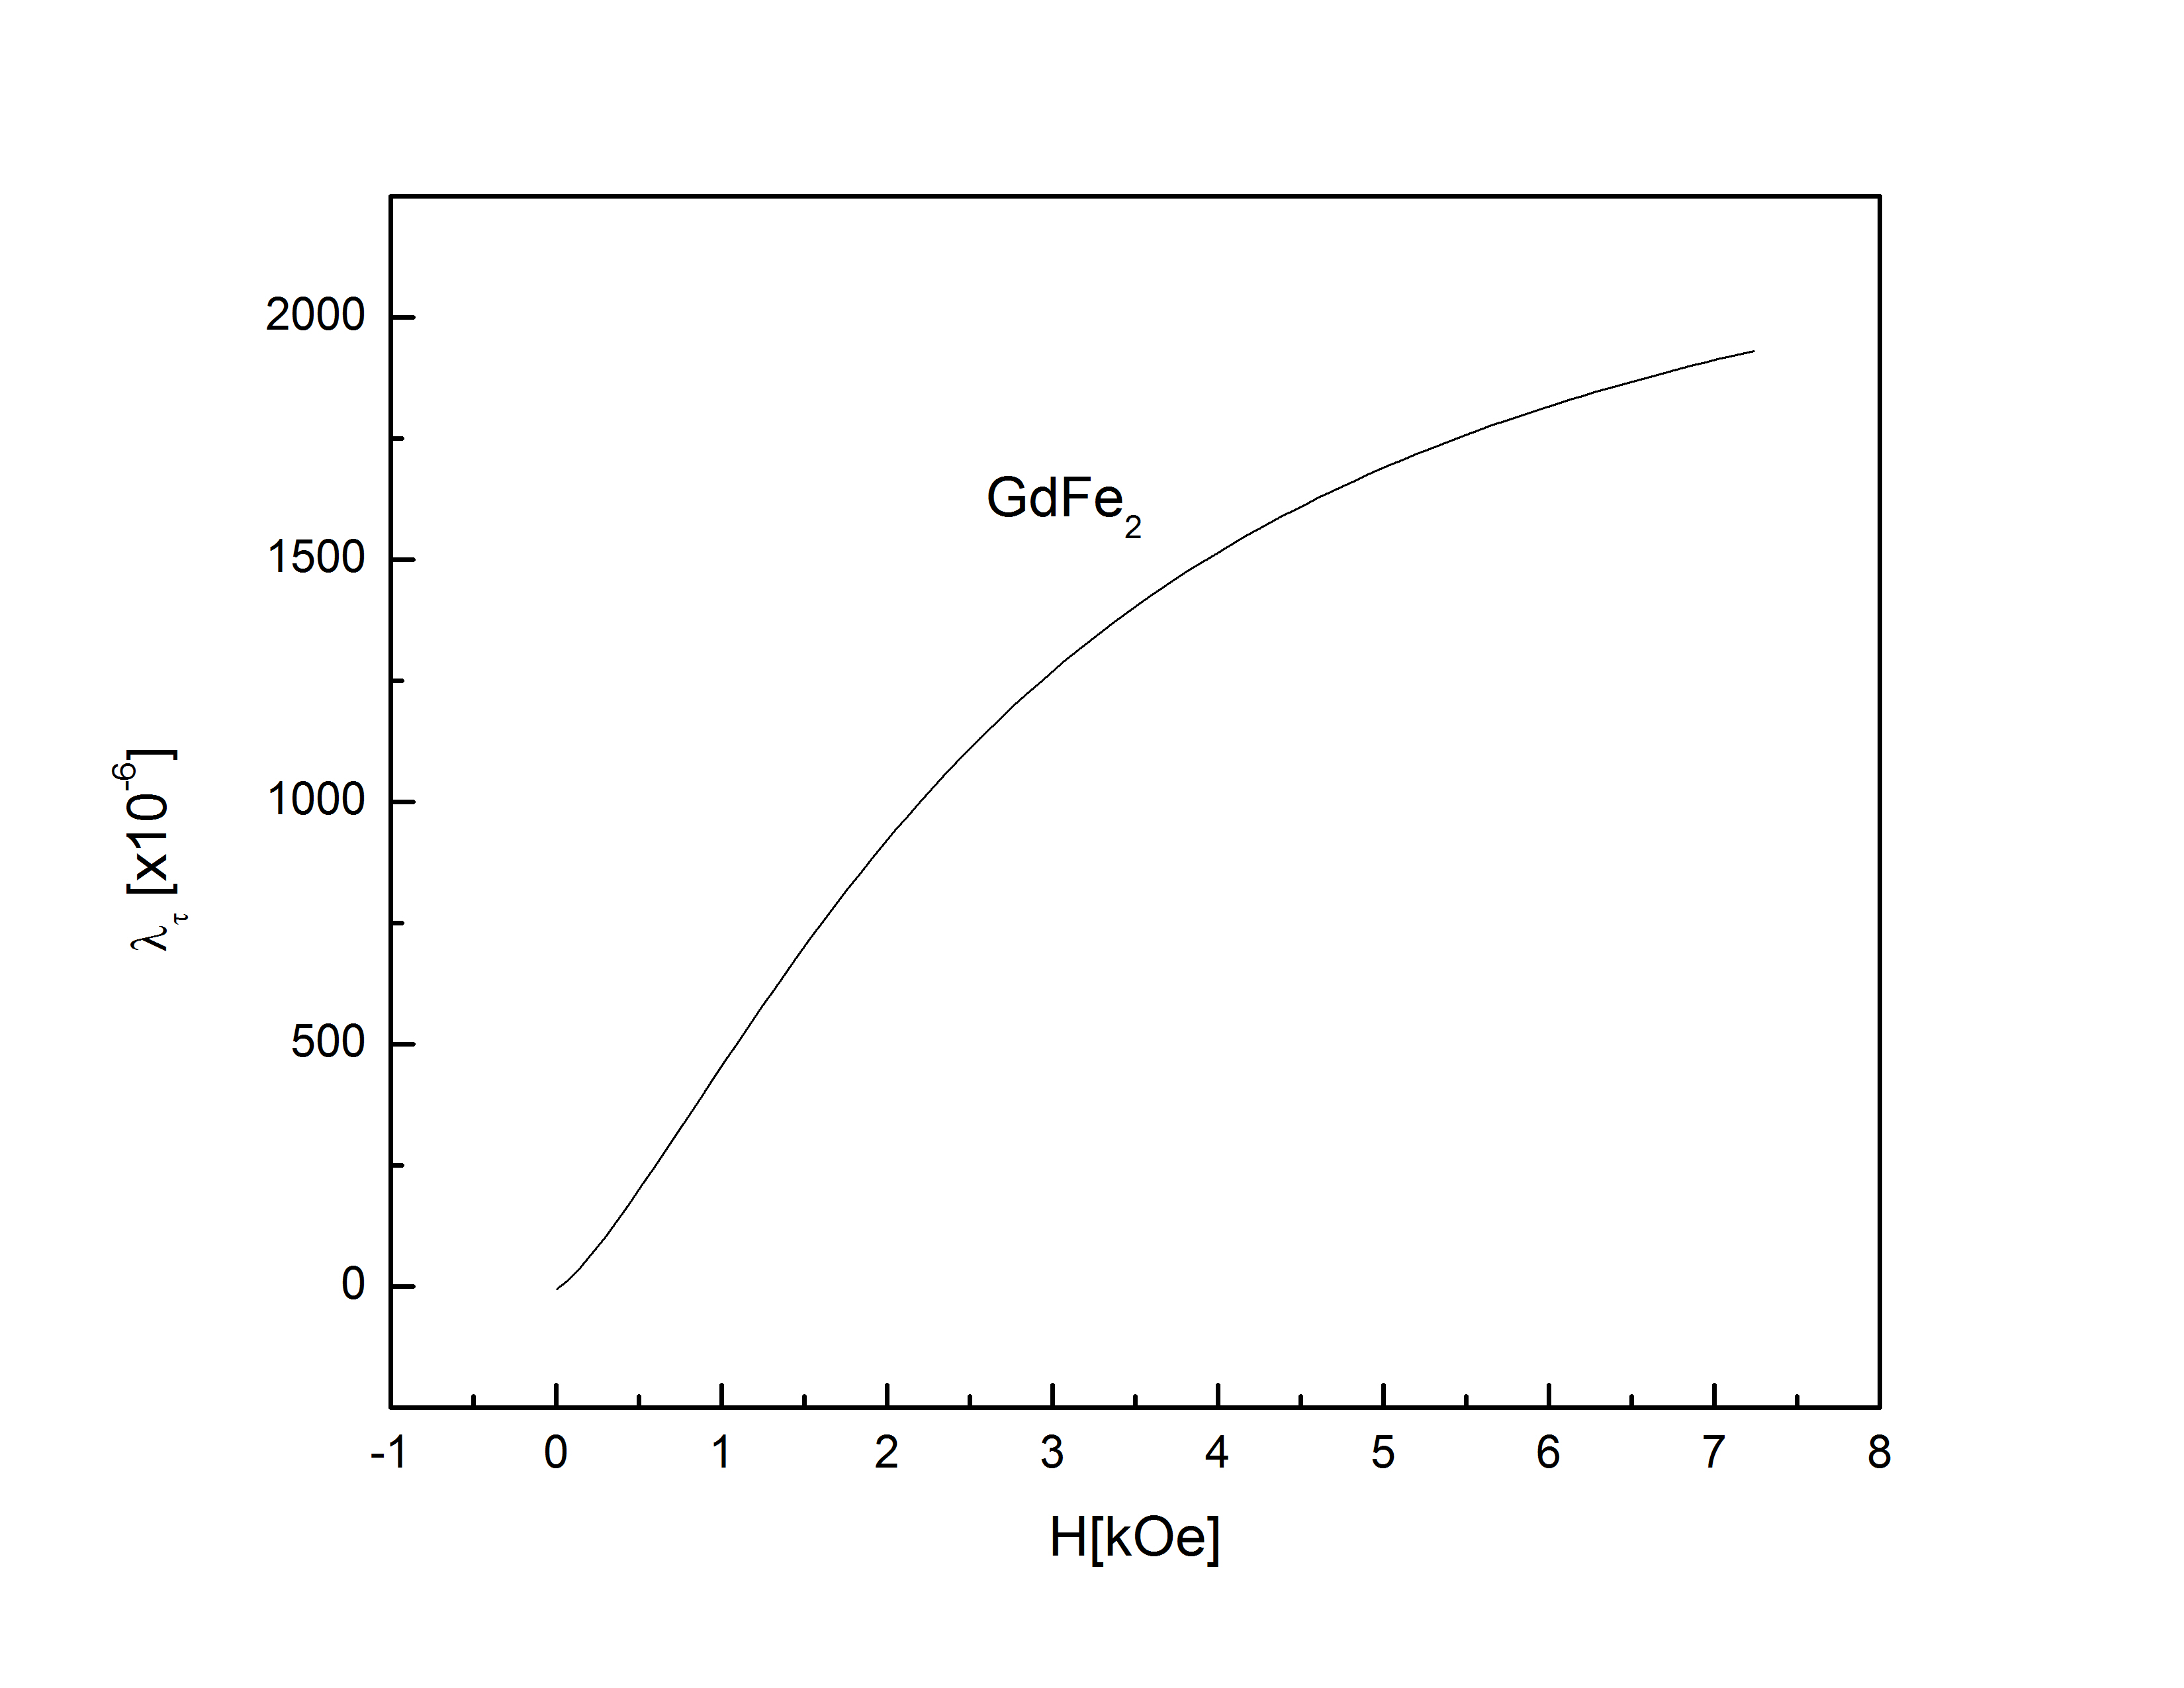
\includegraphics[width =0.9\textwidth]{../img/magneto/GdKsztaltu}
    \caption{Wartość magnetostrykcji kształru $\lambda_{\tau}$ $GdFe_2$}
    \label{GdKsztaltu}
\end{figure}

\begin{figure}[h]
    \centering
    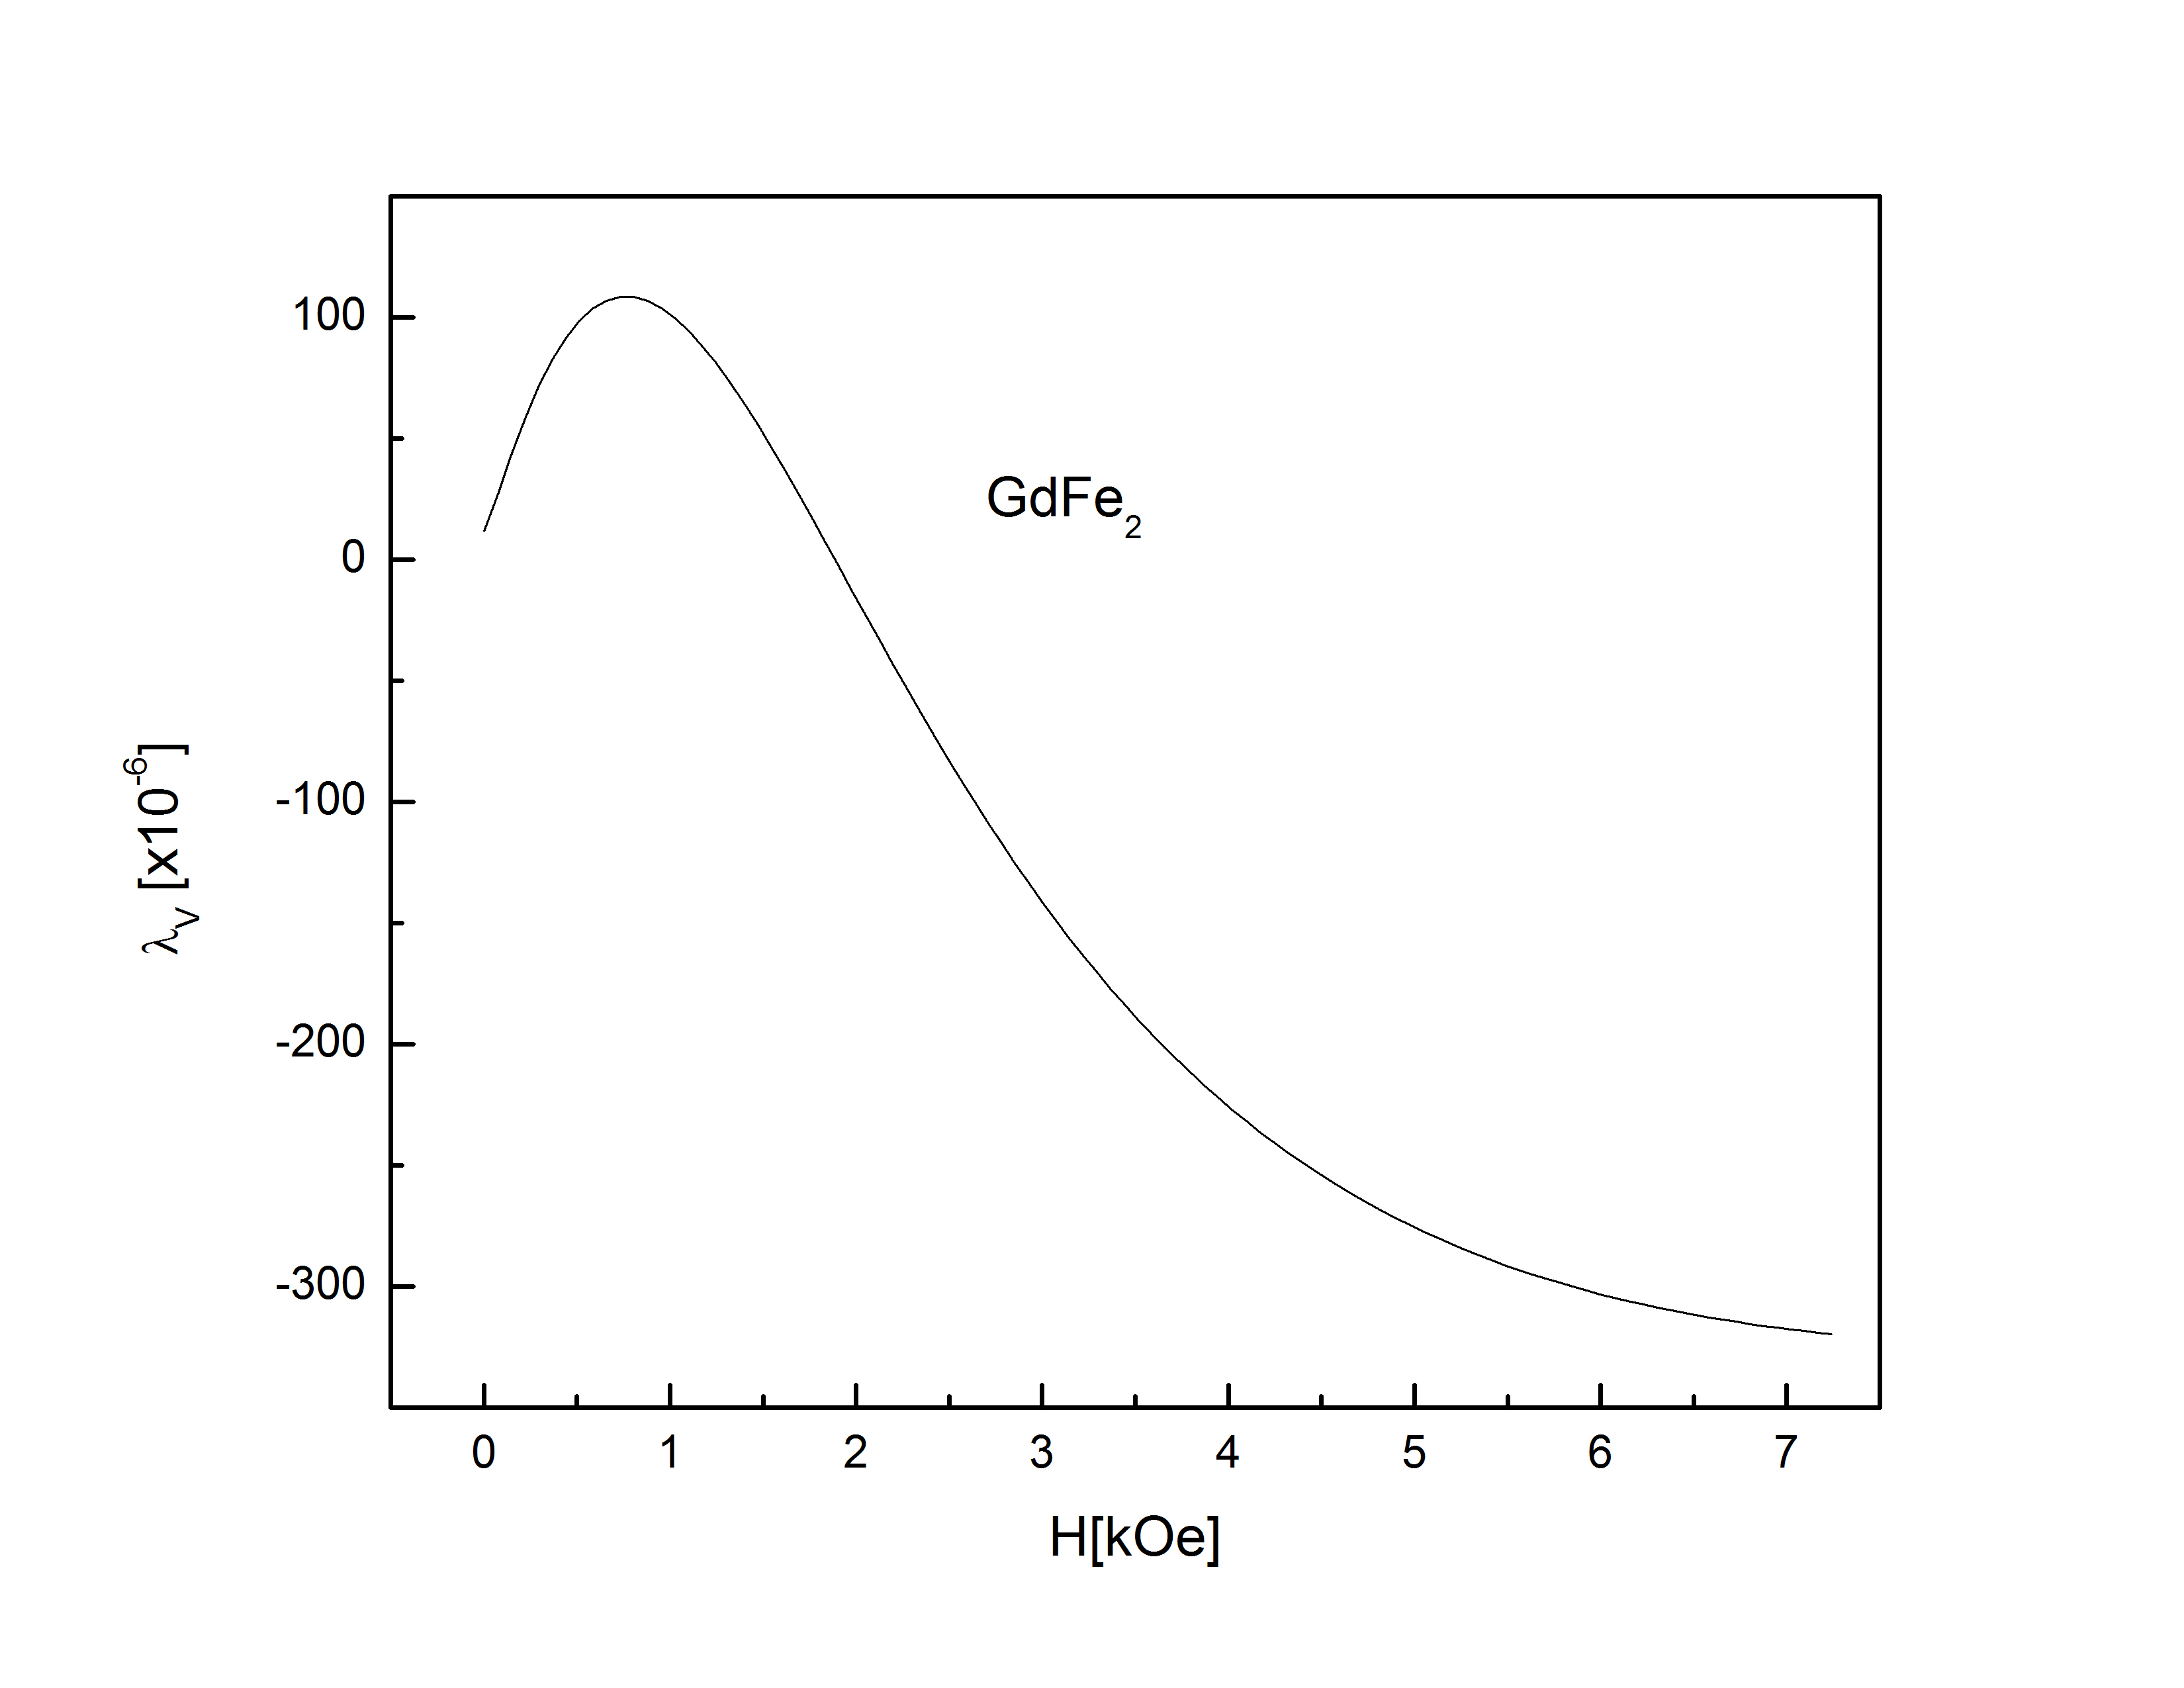
\includegraphics[width =0.9\textwidth]{../img/magneto/GdObjetosc}
    \caption{Wartość magnetostrykcji objetości $\lambda_{V}$ $GdFe_2$}
    \label{GdObjetosc}
\end{figure}

\newpage



\clearpage
\newpage
%\begin{appendices}
\renewcommand{\thetable}{\Alph{section}.\arabic{table}}

%---------------------------------------Ho-------------------------------------


\begin{figure}[h]
    \centering
    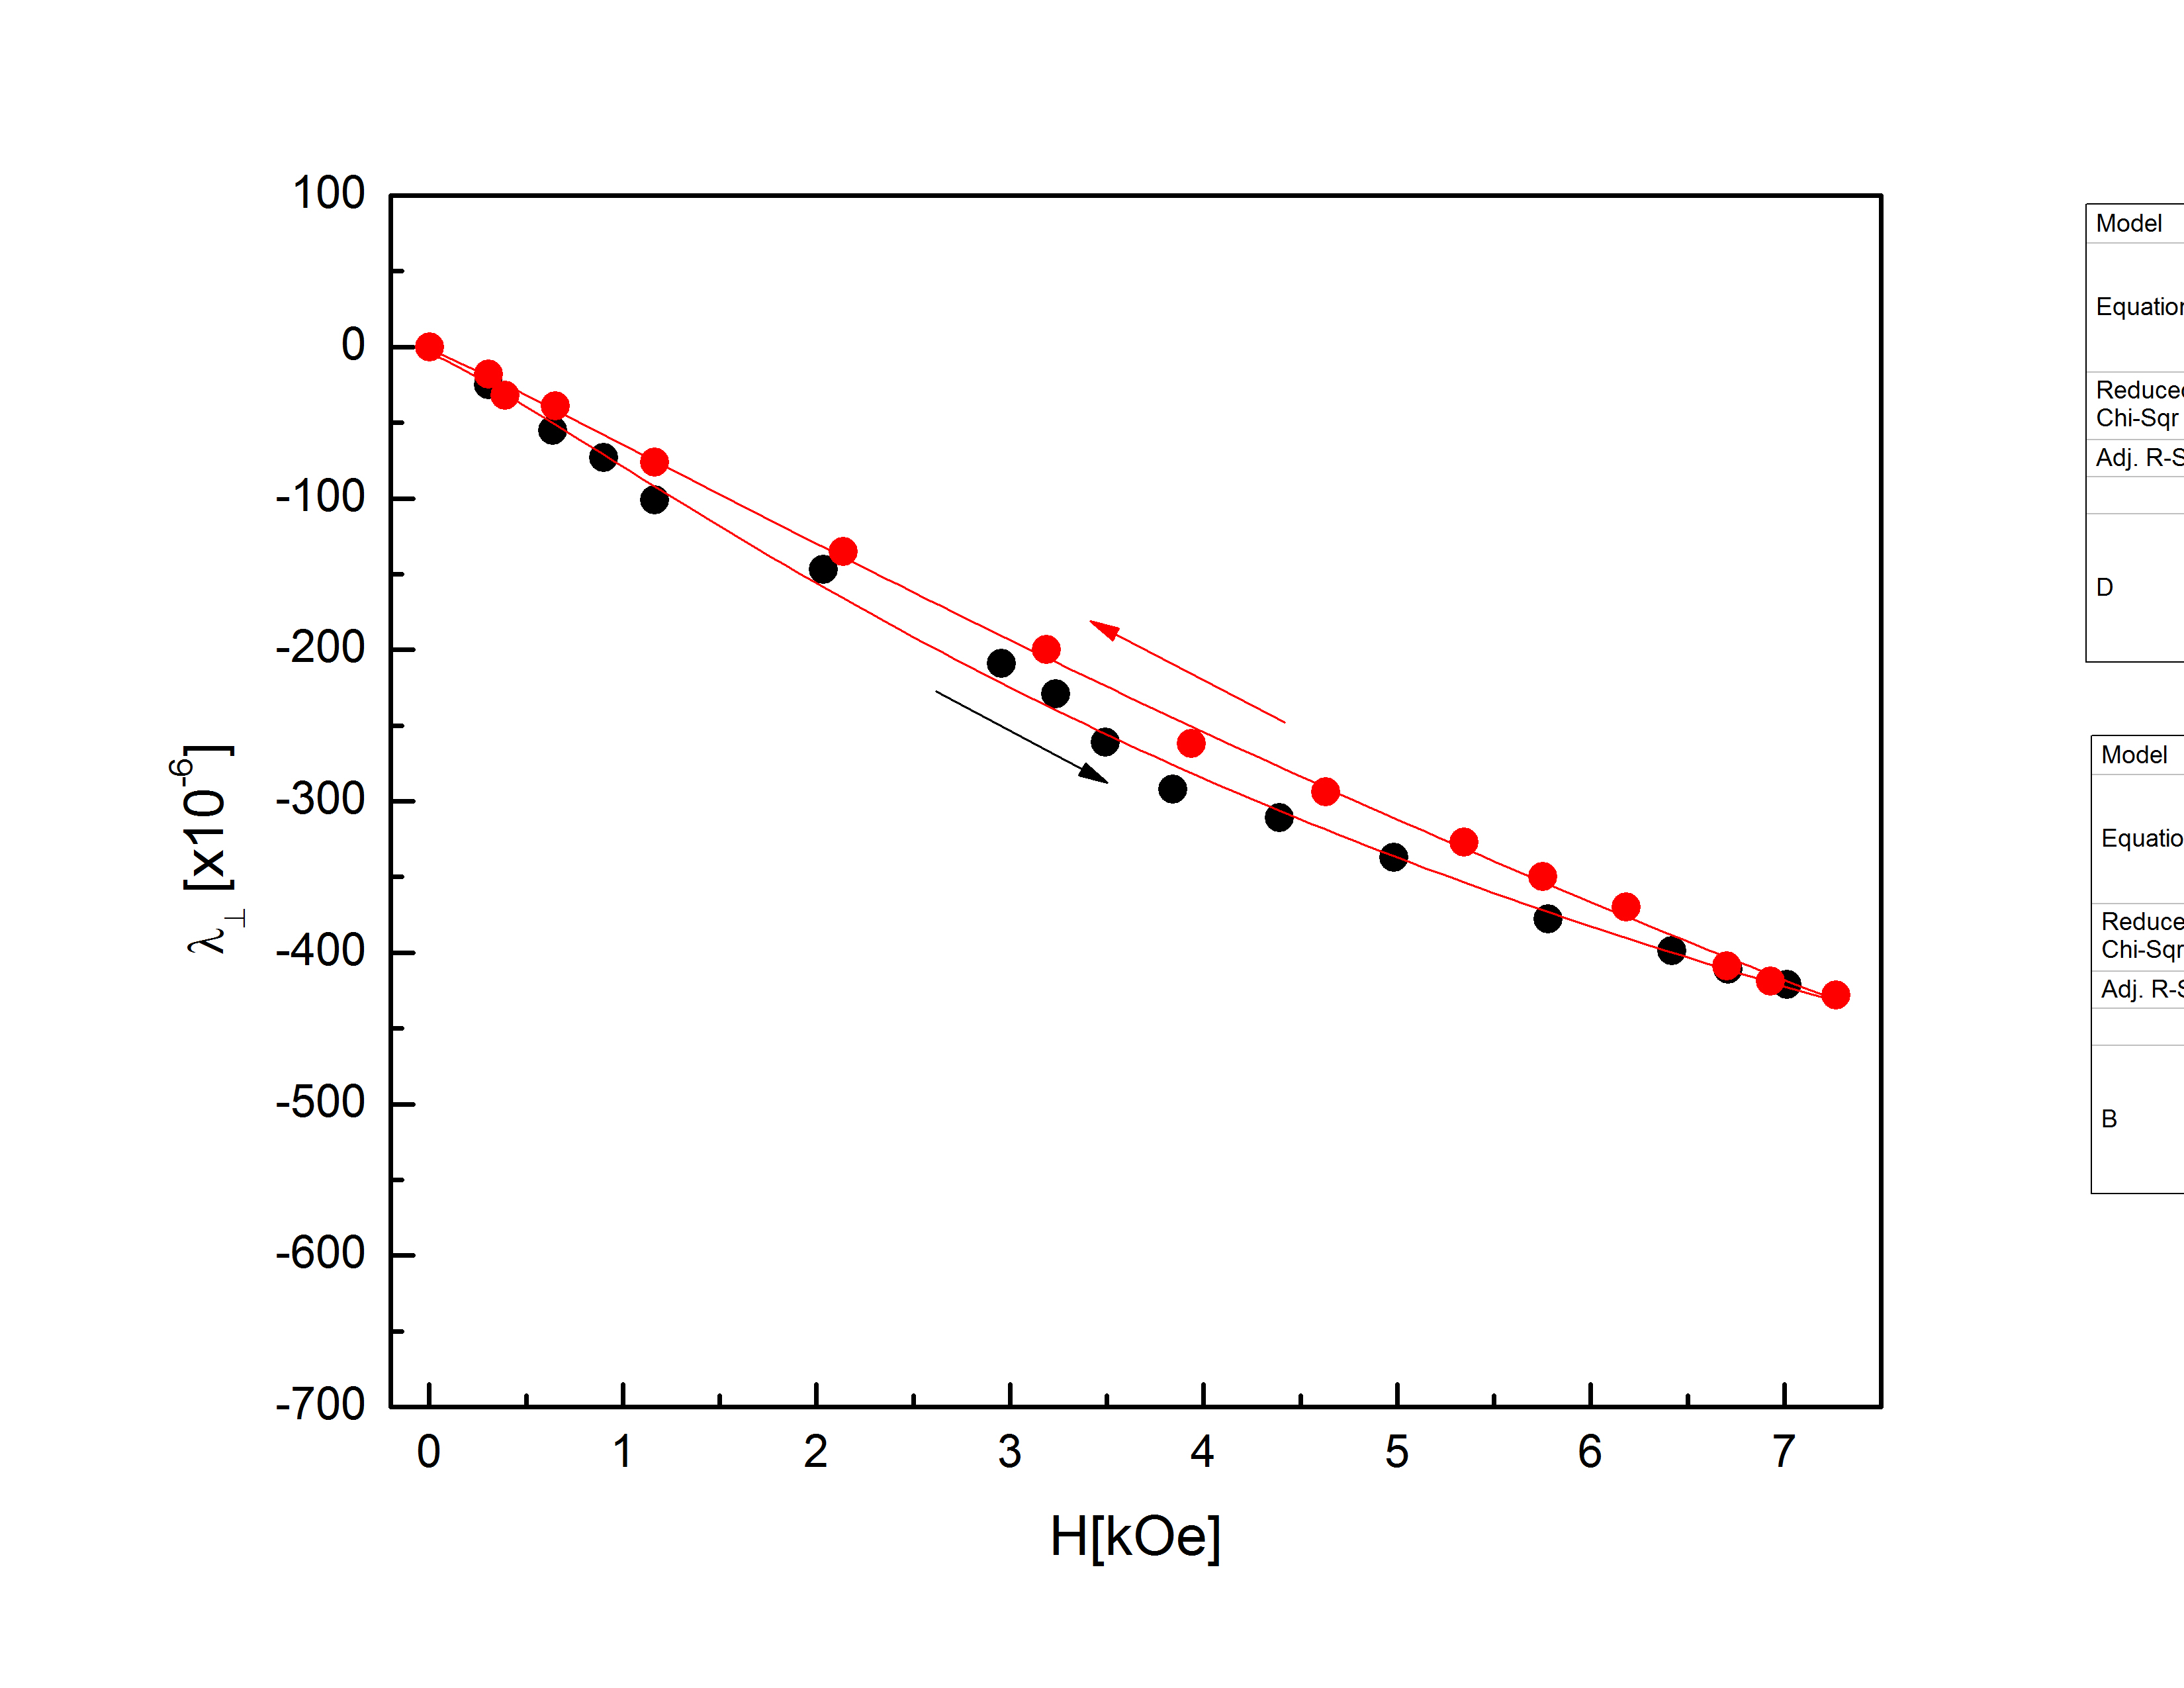
\includegraphics[width =0.9\textwidth]{../img/magneto/Hopoprzeczna}
    \caption{Wartość magnetostrykcji poprzecznej $\lambda_{\perp}$ $HoFe_2$}
    \label{Hopoprzeczna}
\end{figure}

\begin{figure}[h]
    \centering
    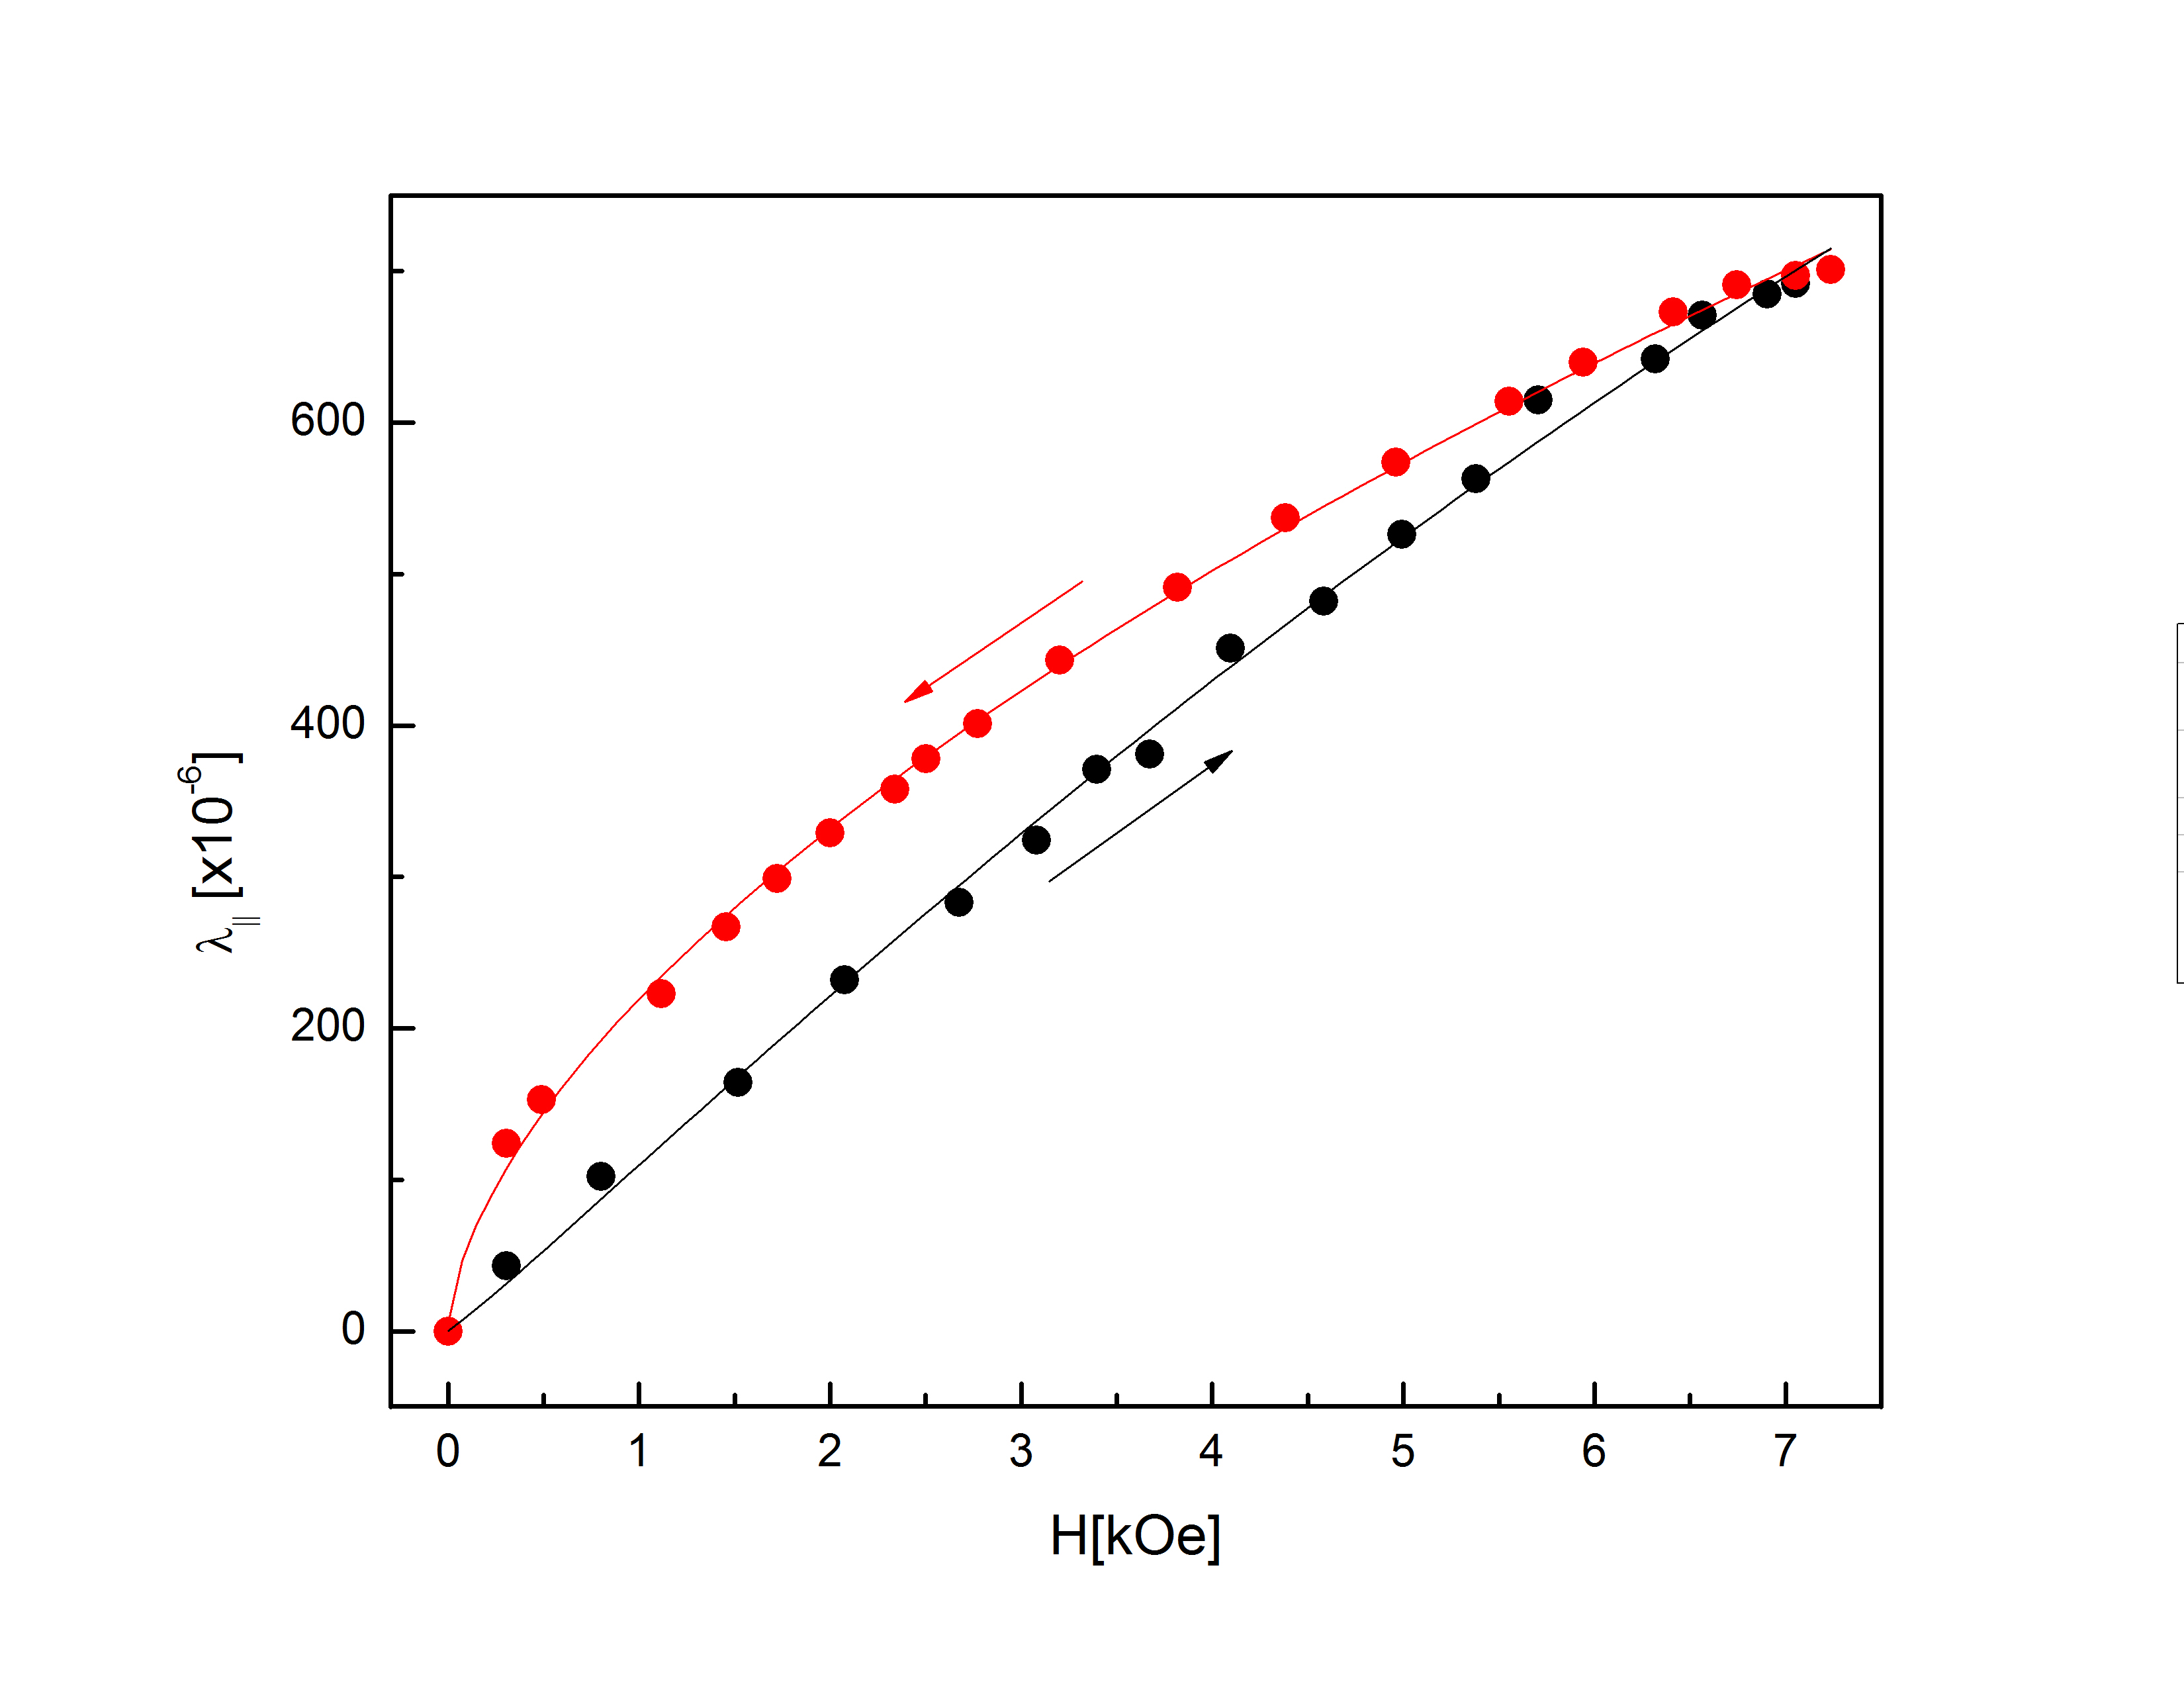
\includegraphics[width =0.9\textwidth]{../img/magneto/Howzdluzna}
    \caption{Wartość magnetostrykcji wzdłużnej $\lambda_{\parallel}$ $HoFe_2$}
    \label{Howzdluzna}
\end{figure}

\begin{figure}[h]
    \centering
    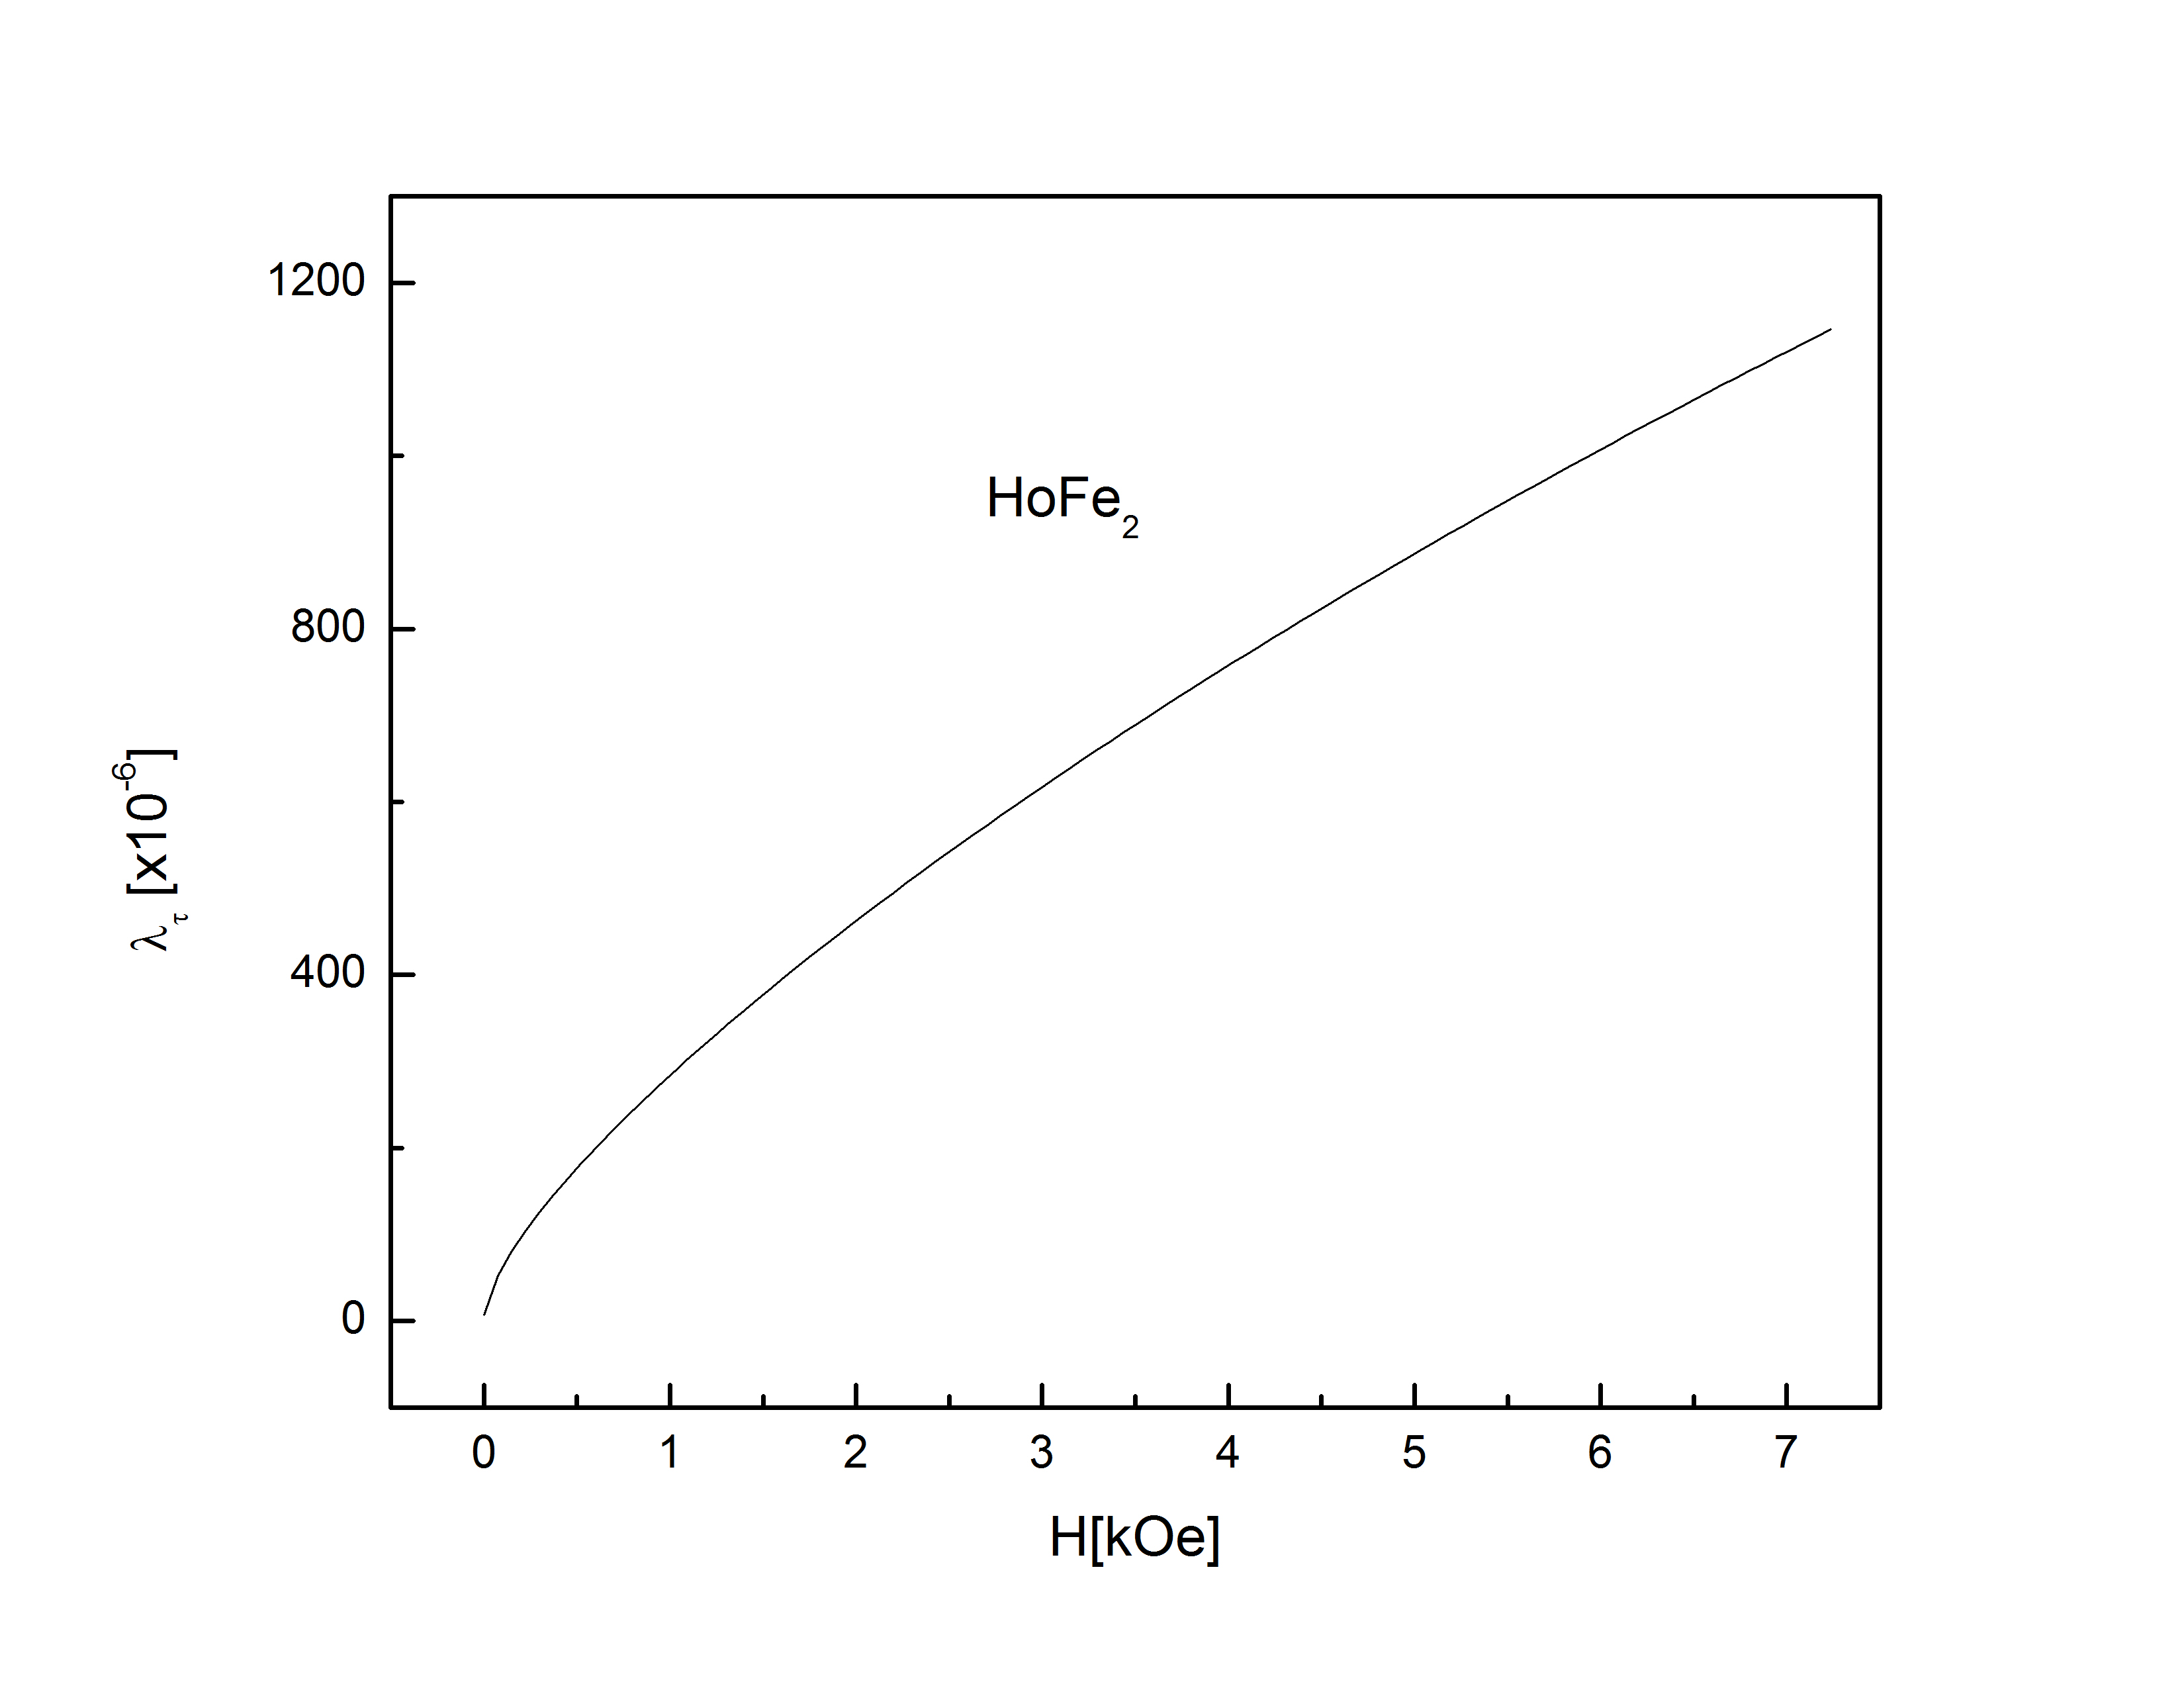
\includegraphics[width =0.9\textwidth]{../img/magneto/HoKsztaltu}
    \caption{Wartość magnetostrykcji kształru $\lambda_{\tau}$ $HoFe_2$}
    \label{HoKsztaltu}
\end{figure}

\begin{figure}[h]
    \centering
    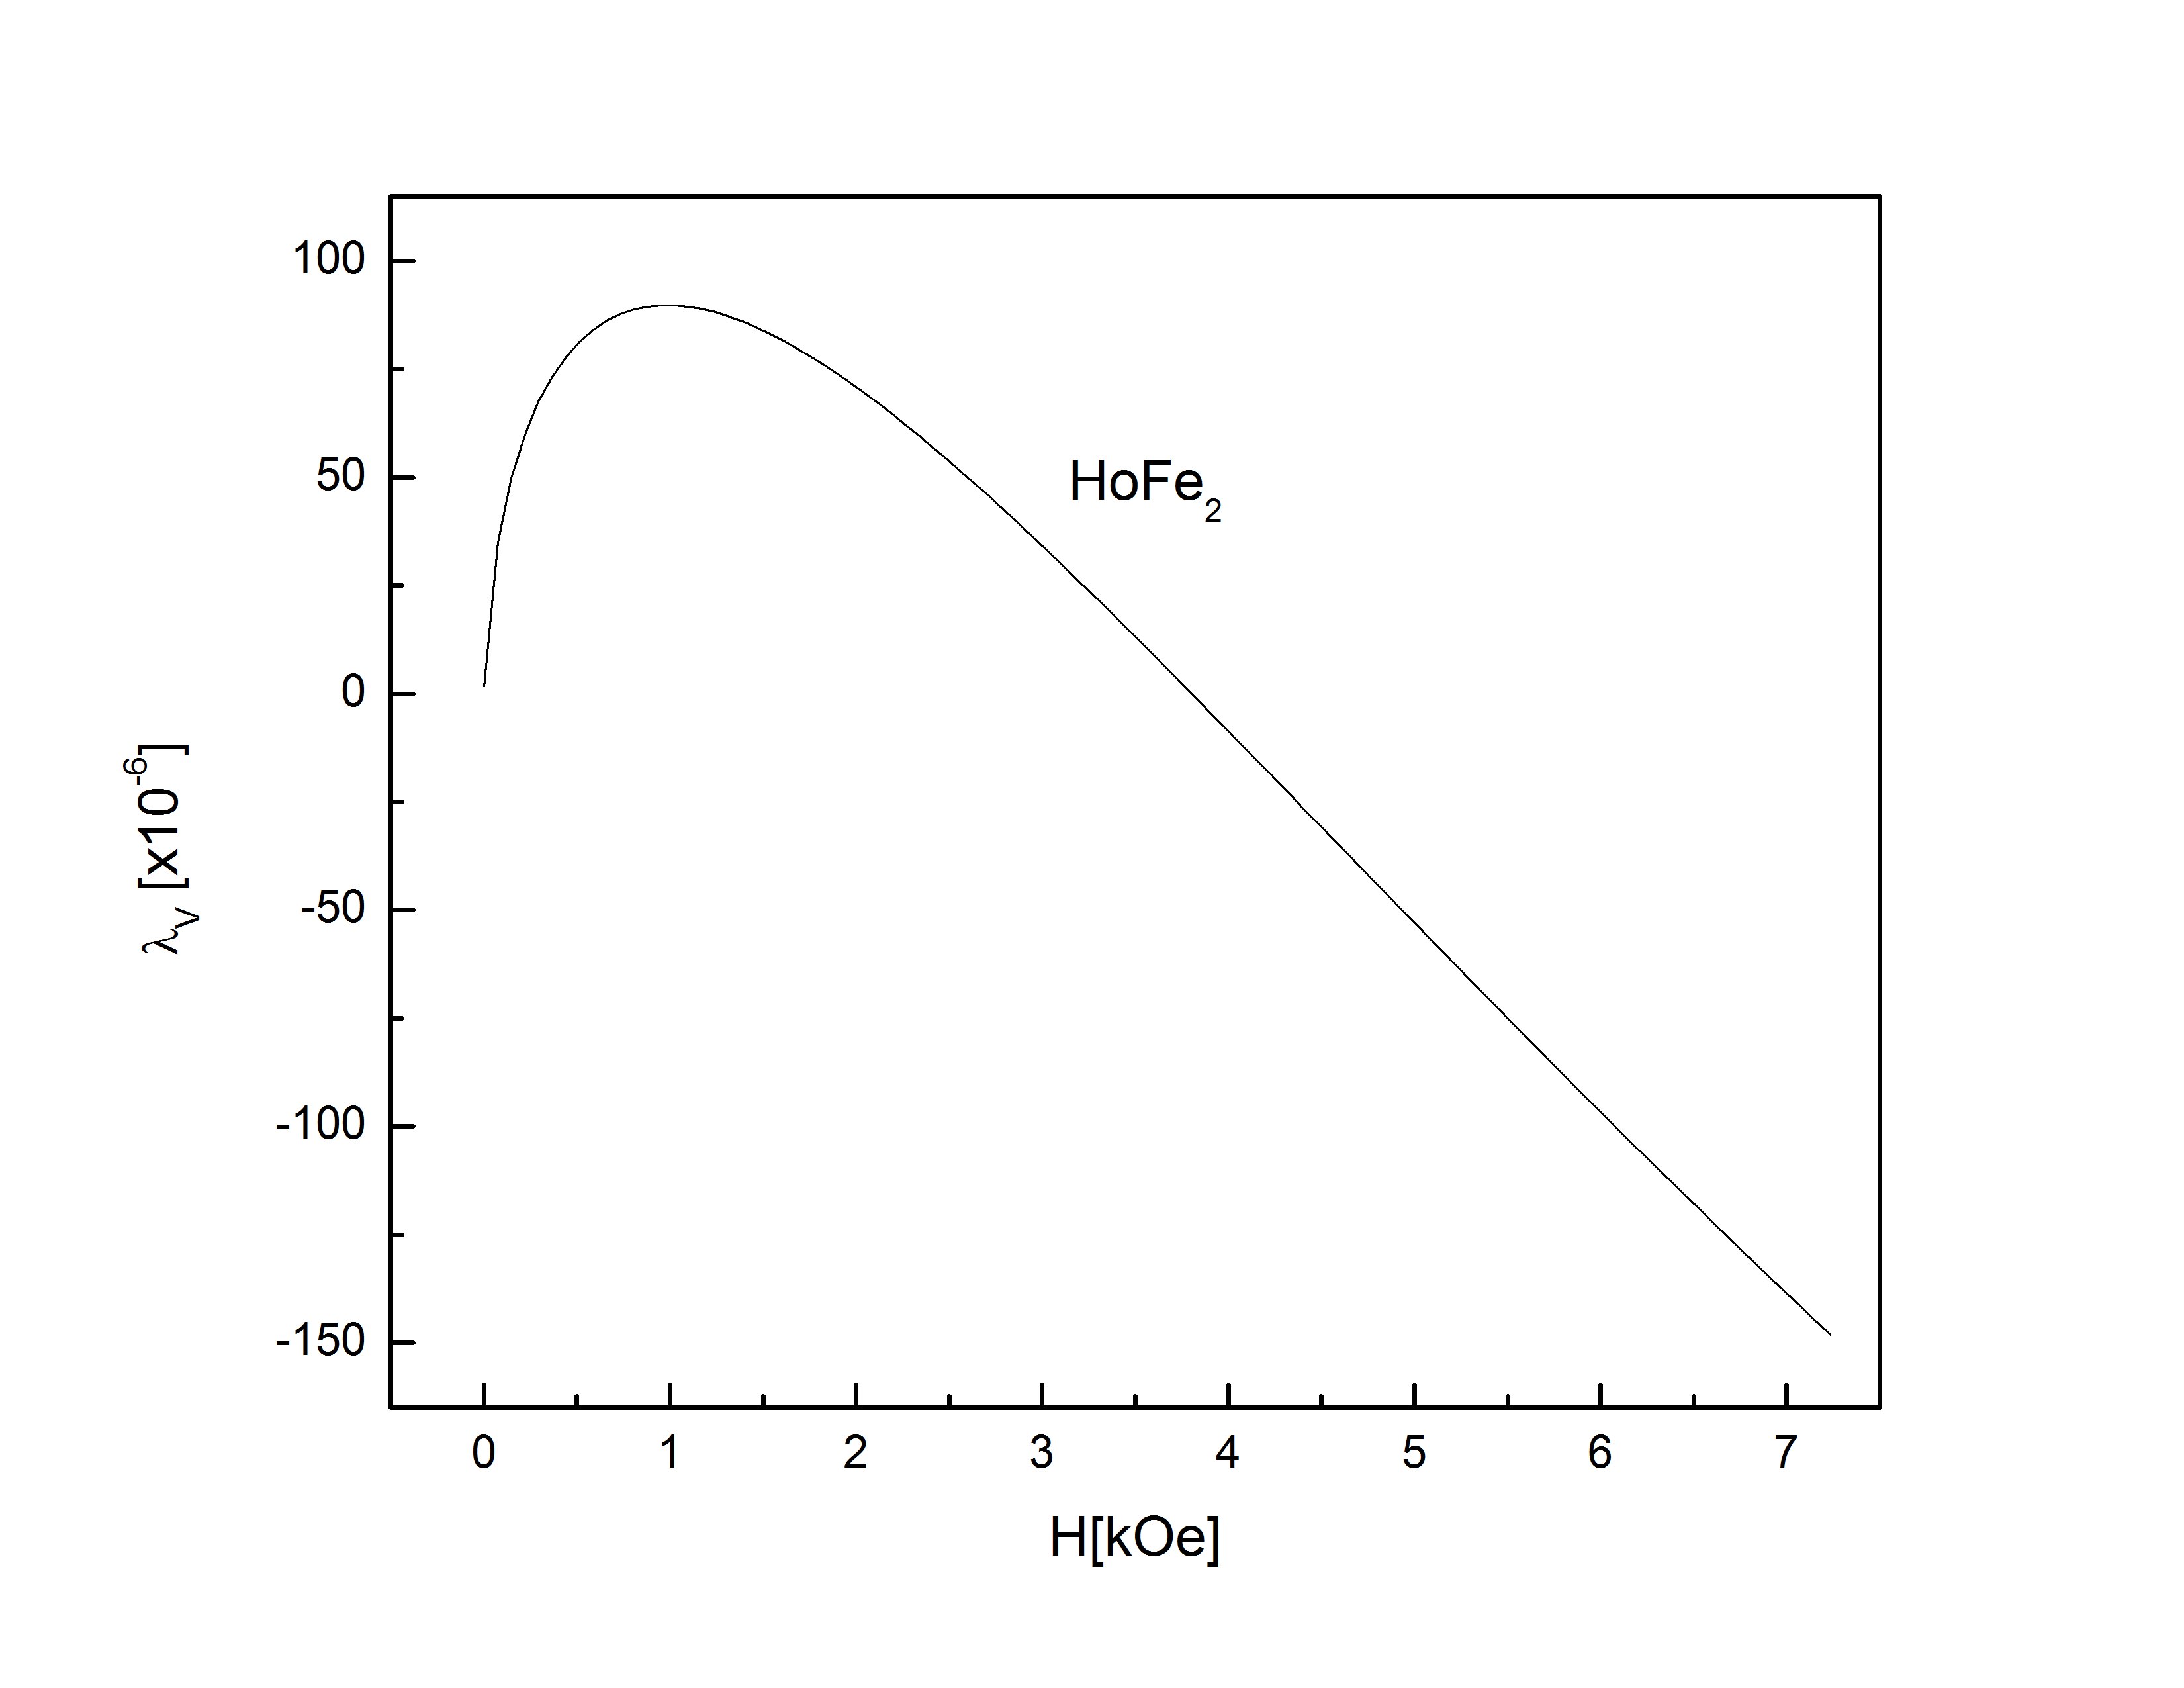
\includegraphics[width =0.9\textwidth]{../img/magneto/HoObjetosc}
    \caption{Wartość magnetostrykcji objetości $\lambda_{V}$ $HoFe_2$}
    \label{HoObjetosc}
\end{figure}

%---------------------------------------Tb-------------------------------------


\begin{figure}[h]
    \centering
    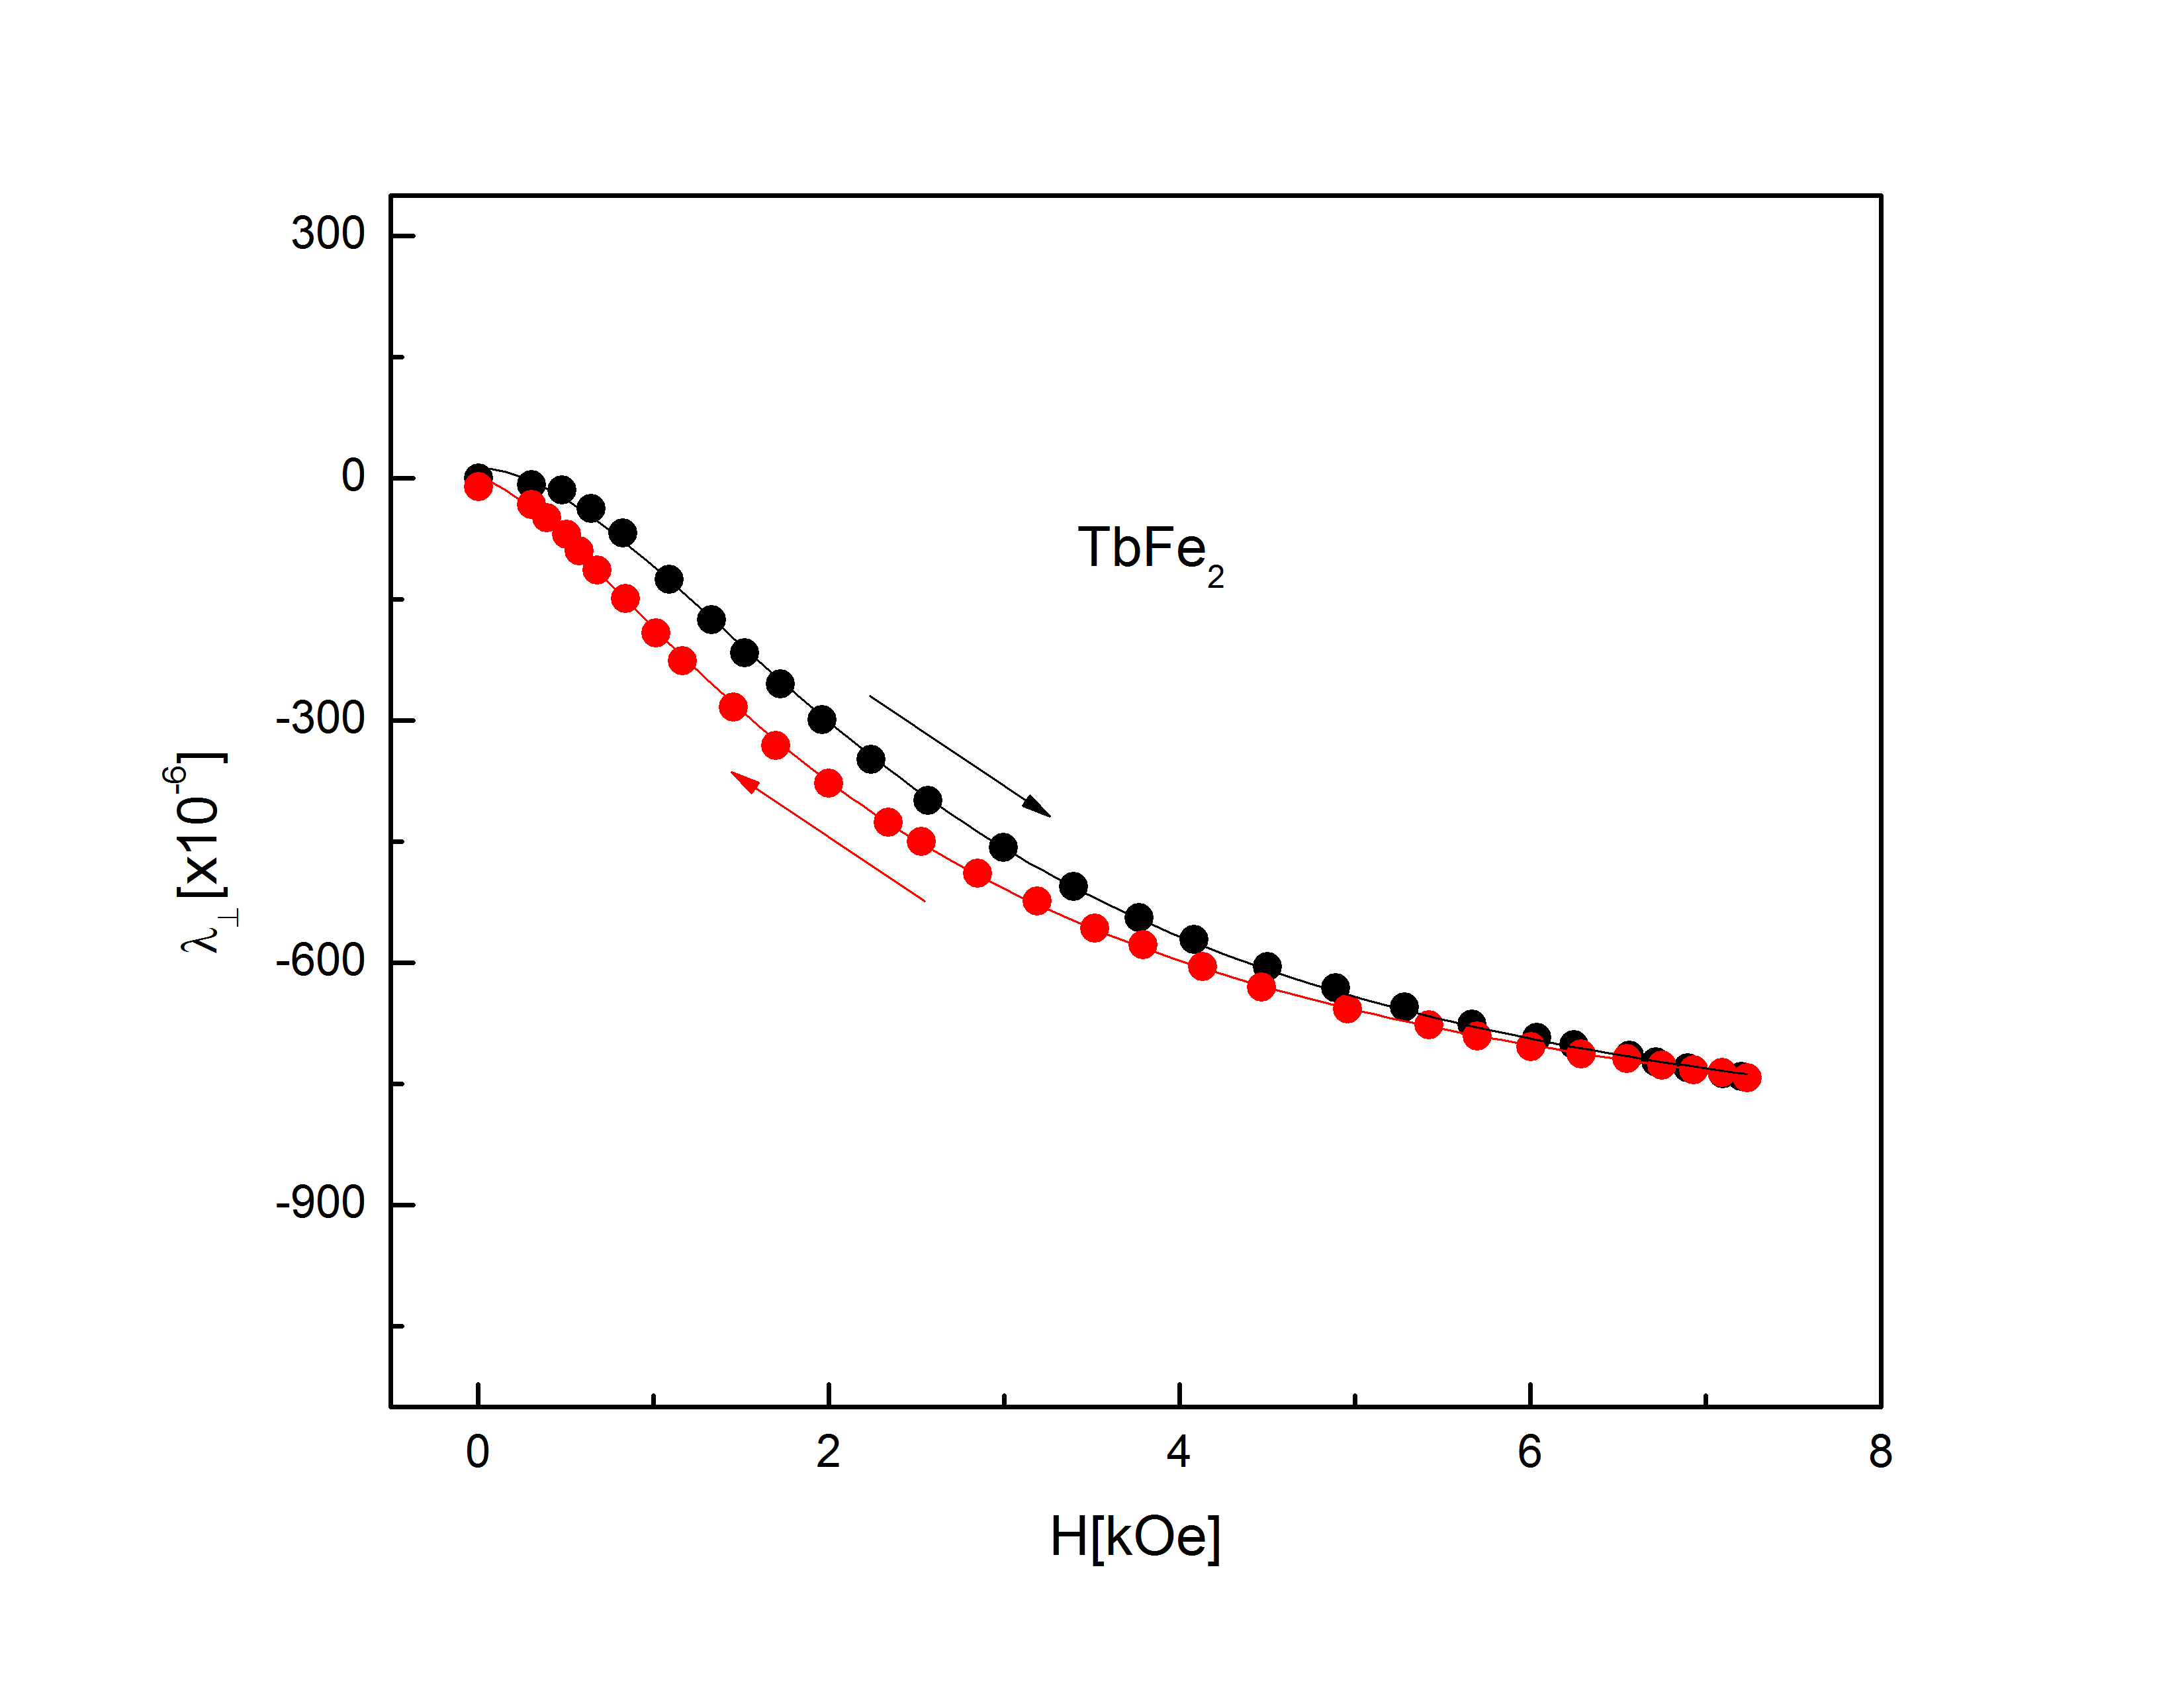
\includegraphics[width =0.9\textwidth]{../img/magneto/Tbpoprzeczna}
    \caption{Wartość magnetostrykcji poprzecznej $\lambda_{\perp}$ $TbFe_2$}
    \label{Tbpoprzeczna}
\end{figure}

\begin{figure}[h]
    \centering
    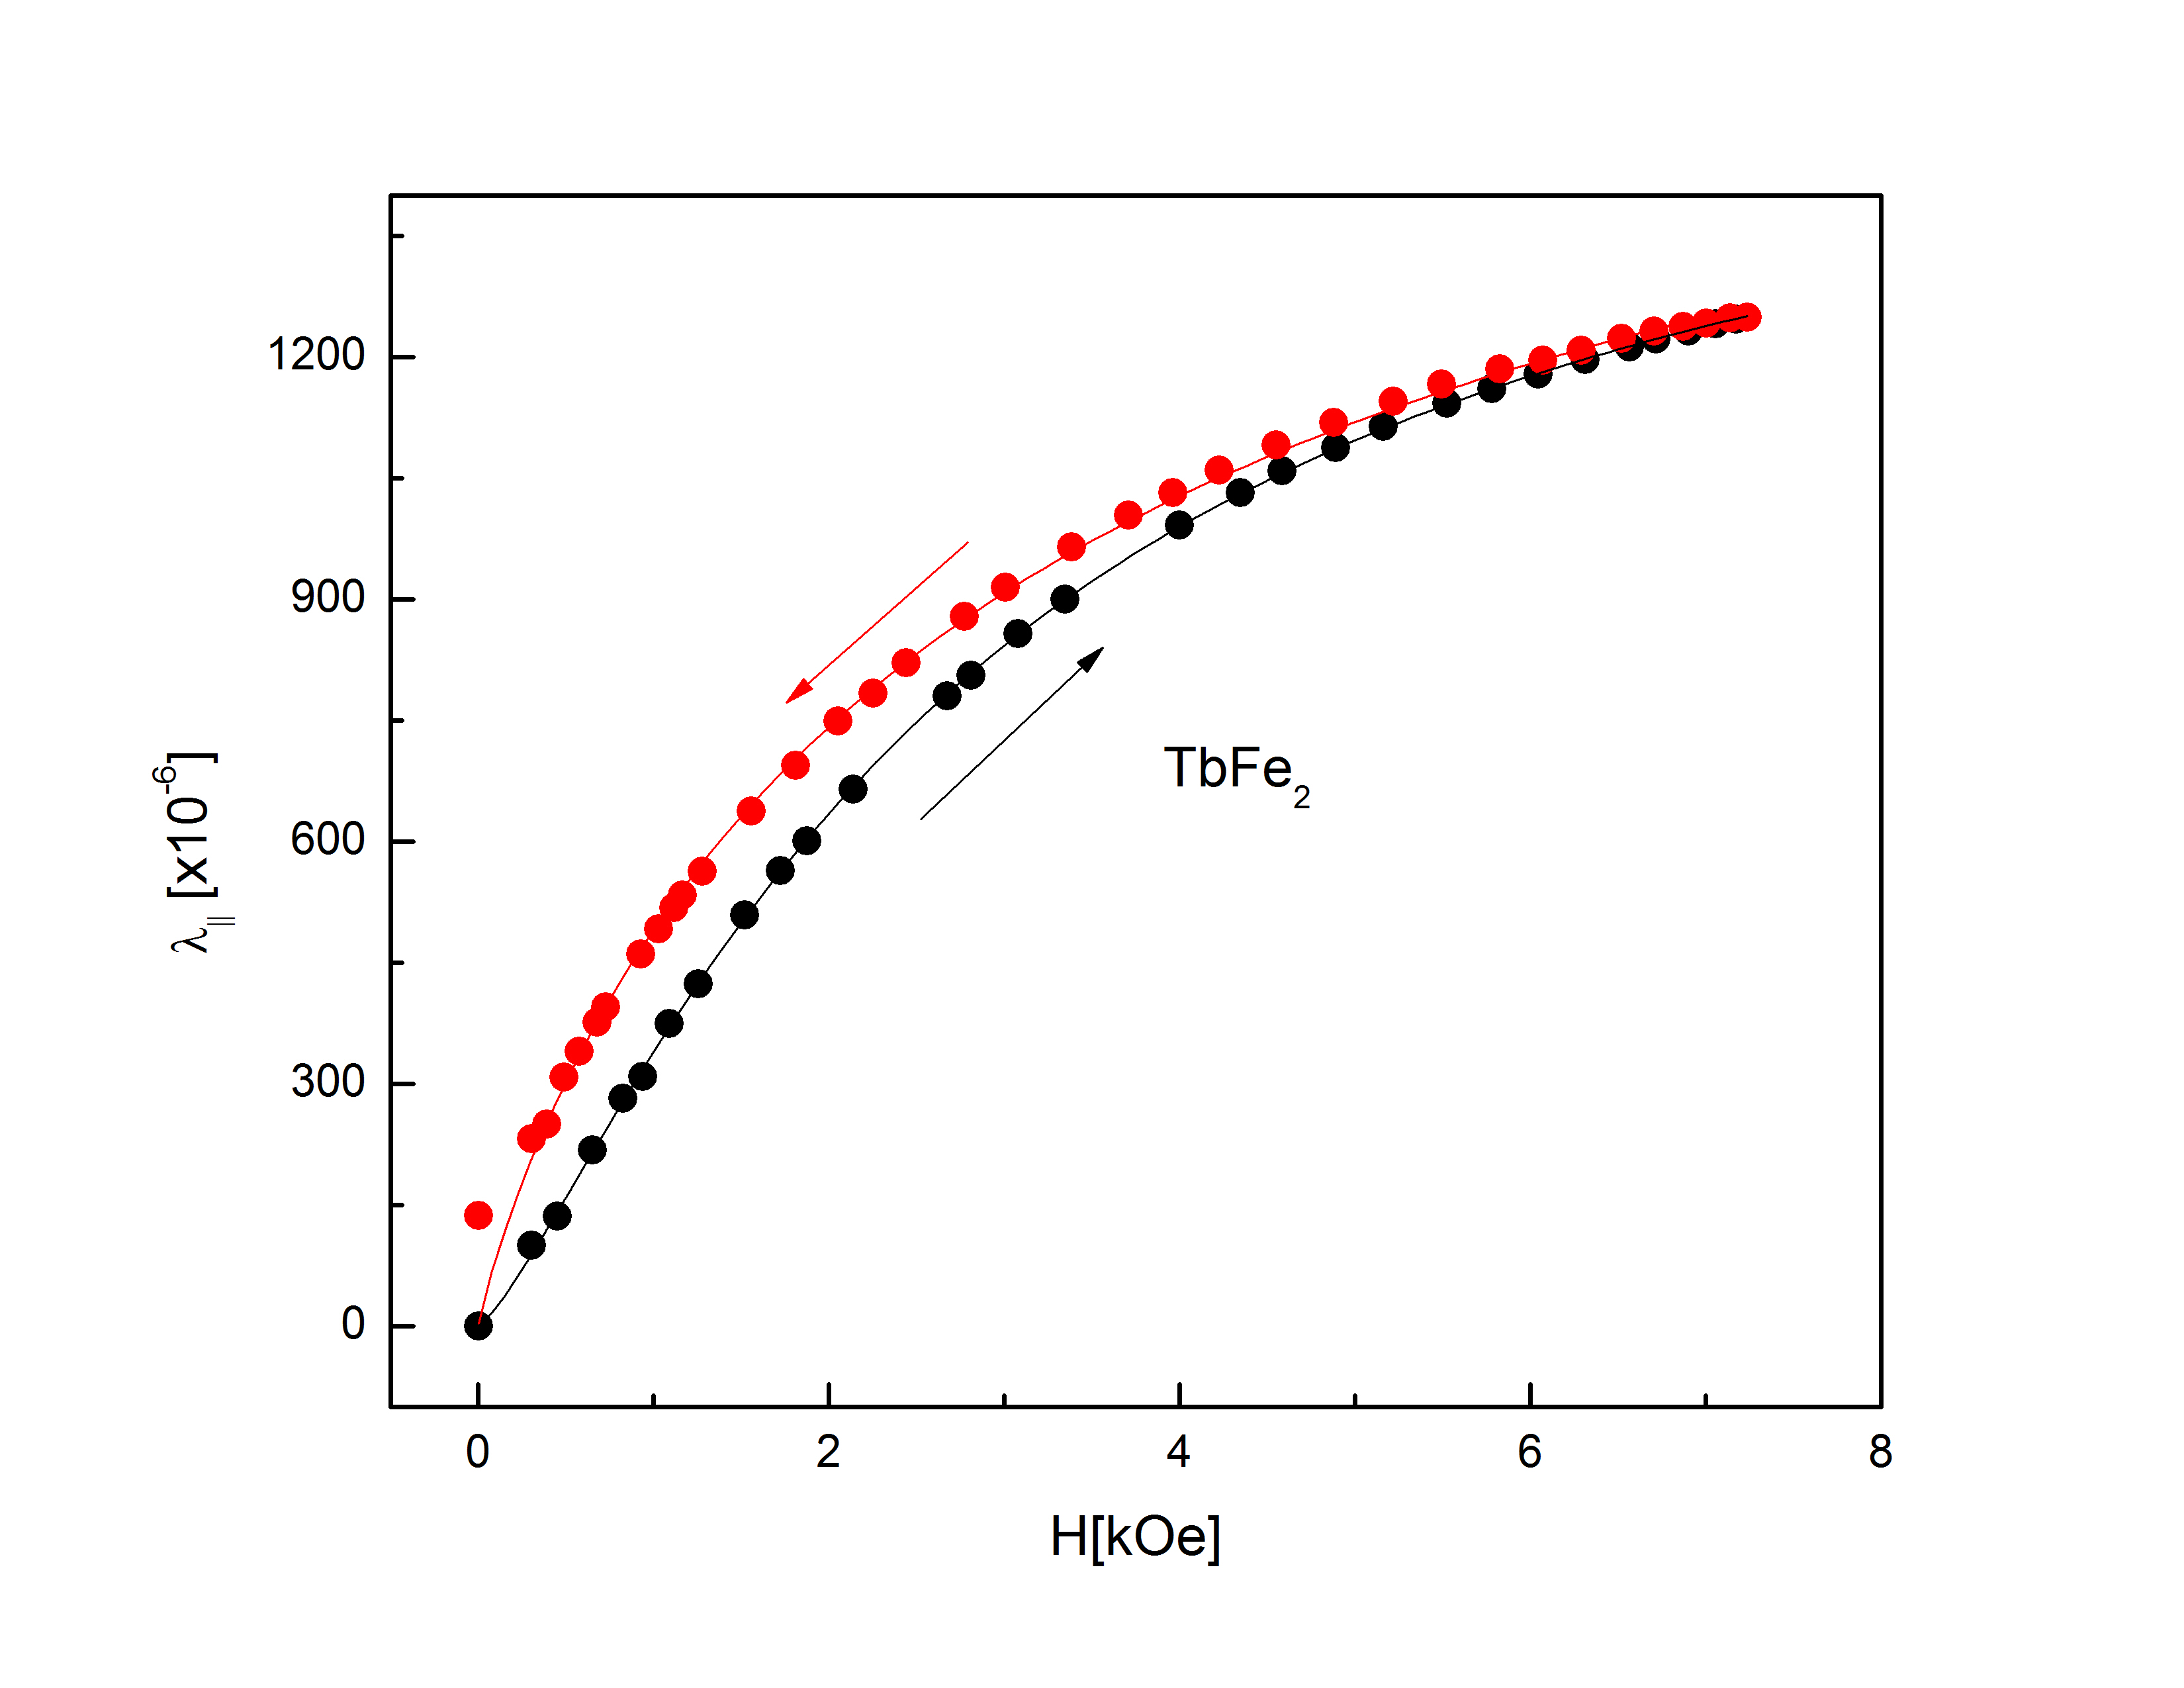
\includegraphics[width =0.9\textwidth]{../img/magneto/Tbwzdluzna}
    \caption{Wartość magnetostrykcji wzdłużnej $\lambda_{\parallel}$ $TbFe_2$}
    \label{Tbwzdluzna}
\end{figure}

\begin{figure}[h]
    \centering
    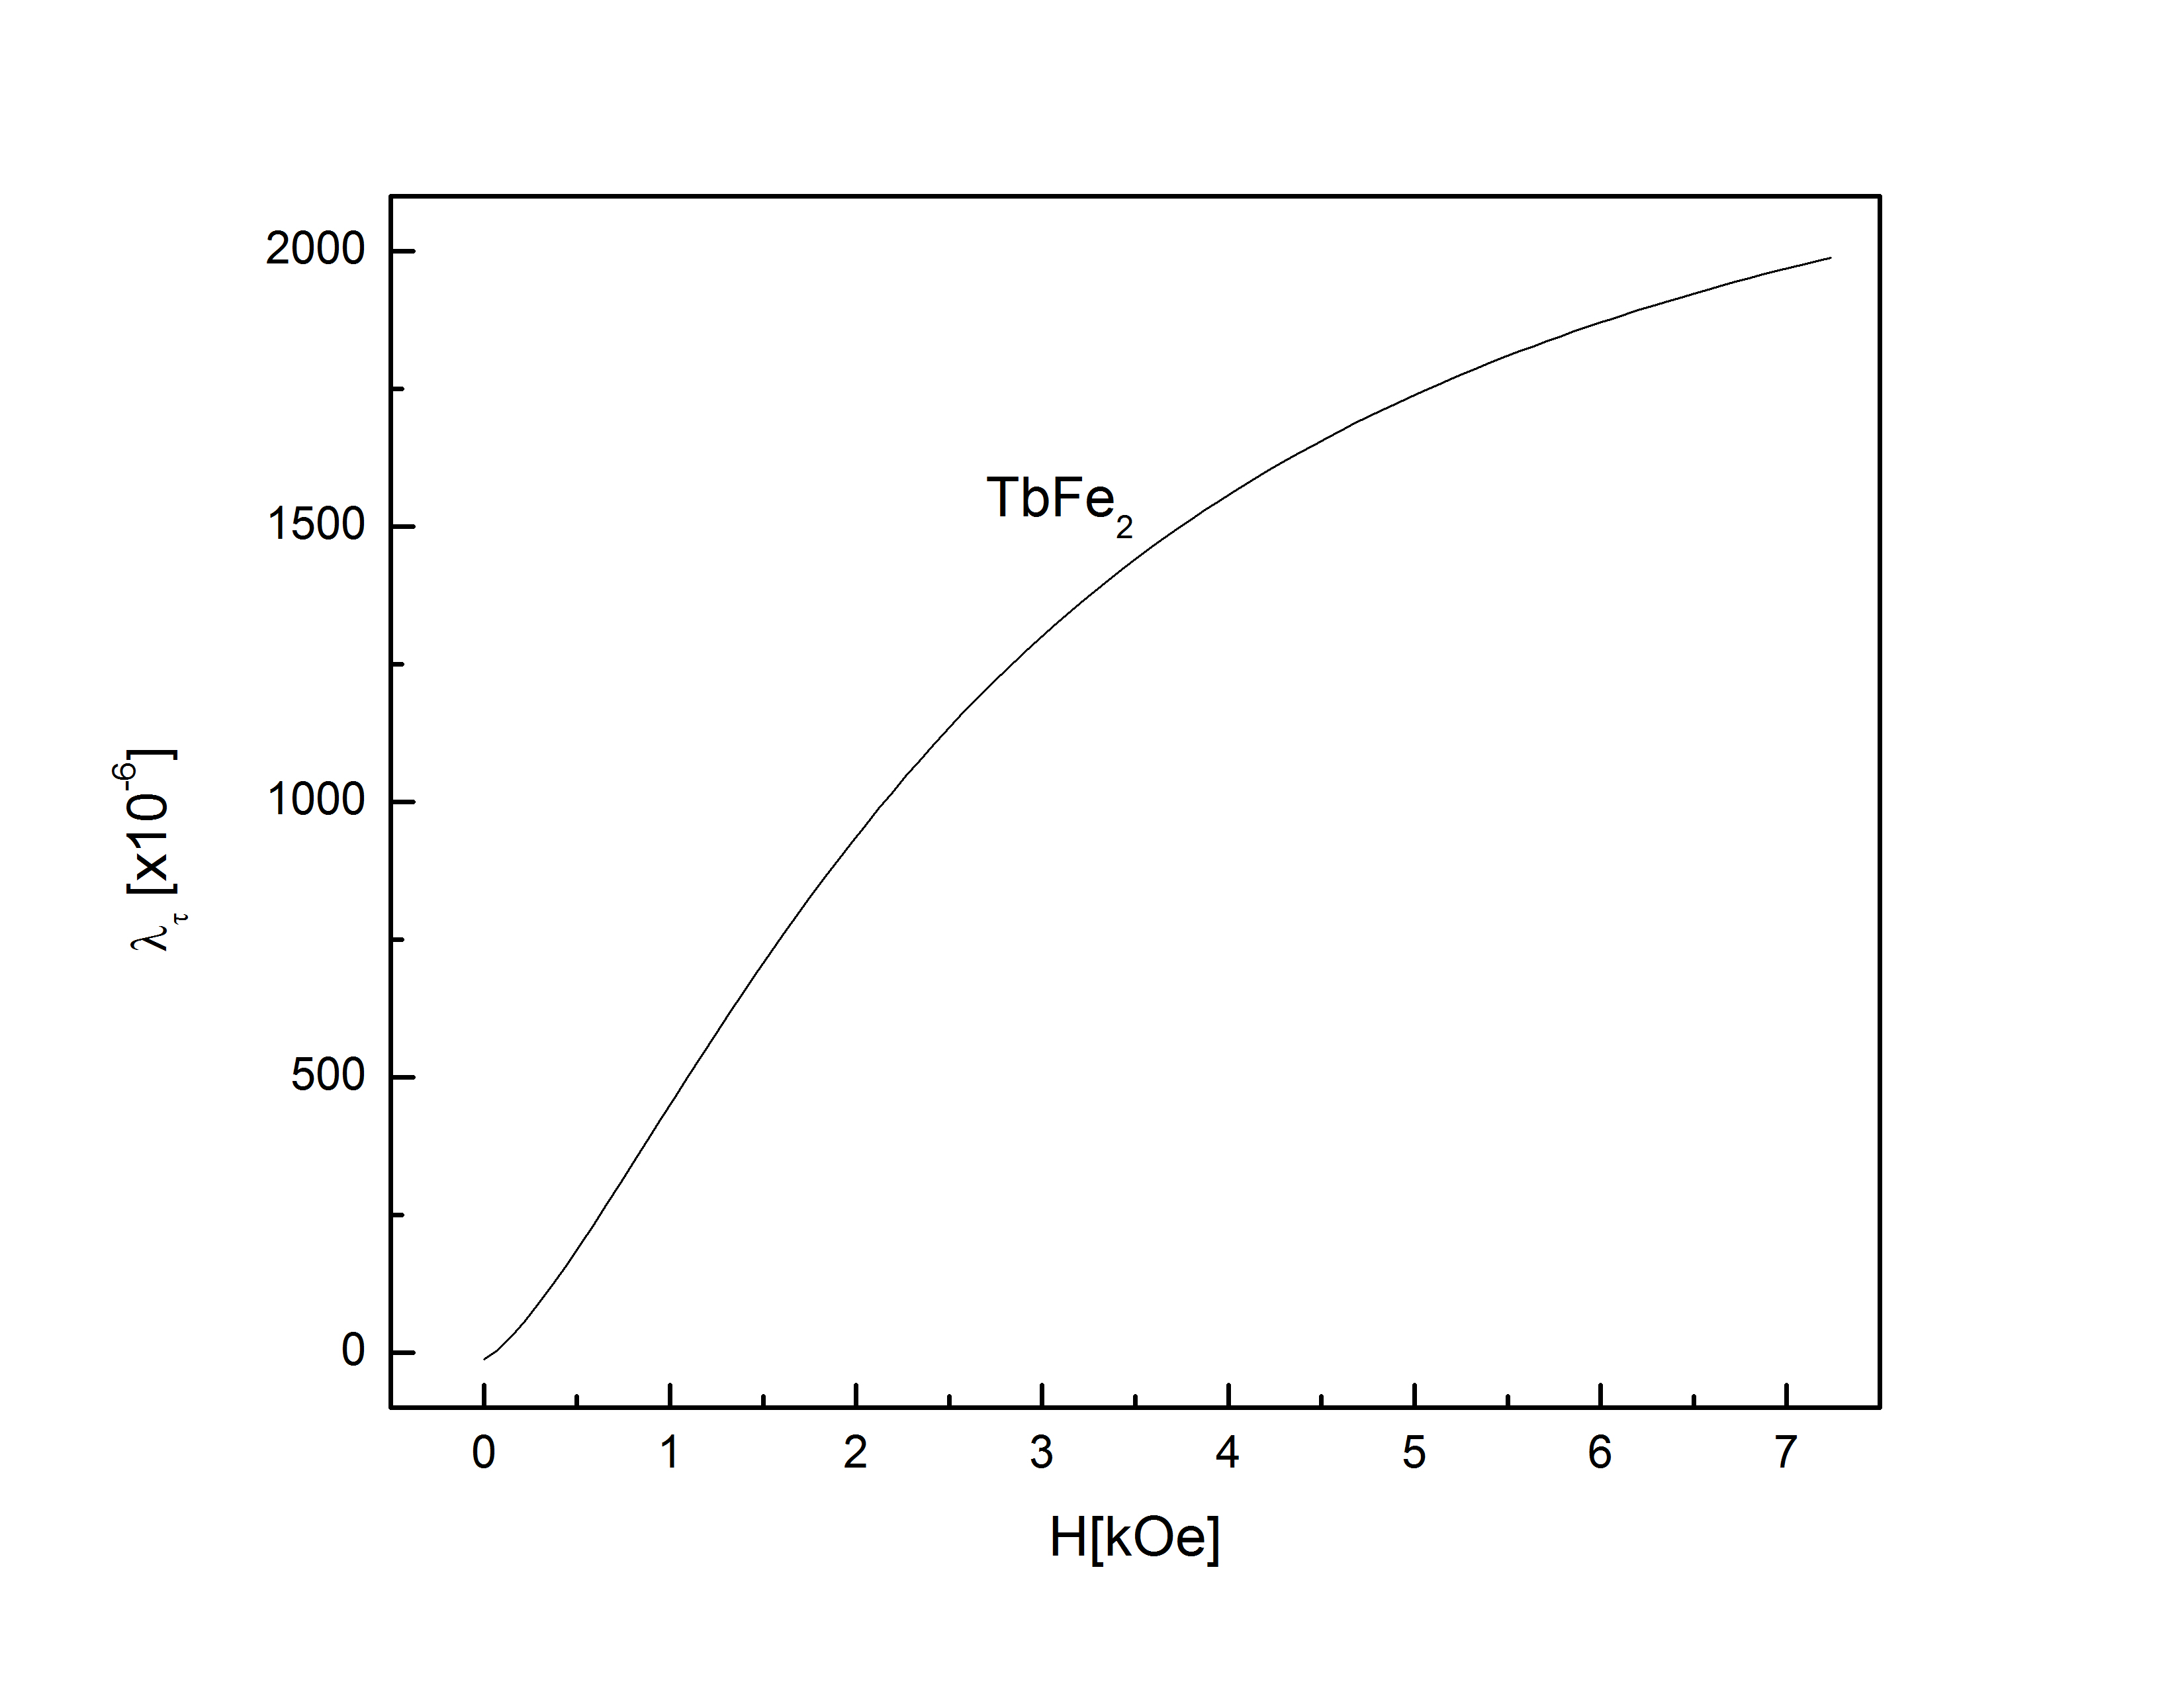
\includegraphics[width =0.9\textwidth]{../img/magneto/TbKsztaltu}
    \caption{Wartość magnetostrykcji kształru $\lambda_{\tau}$ $TbFe_2$}
    \label{TbKsztaltu}
\end{figure}

\begin{figure}[h]
    \centering
    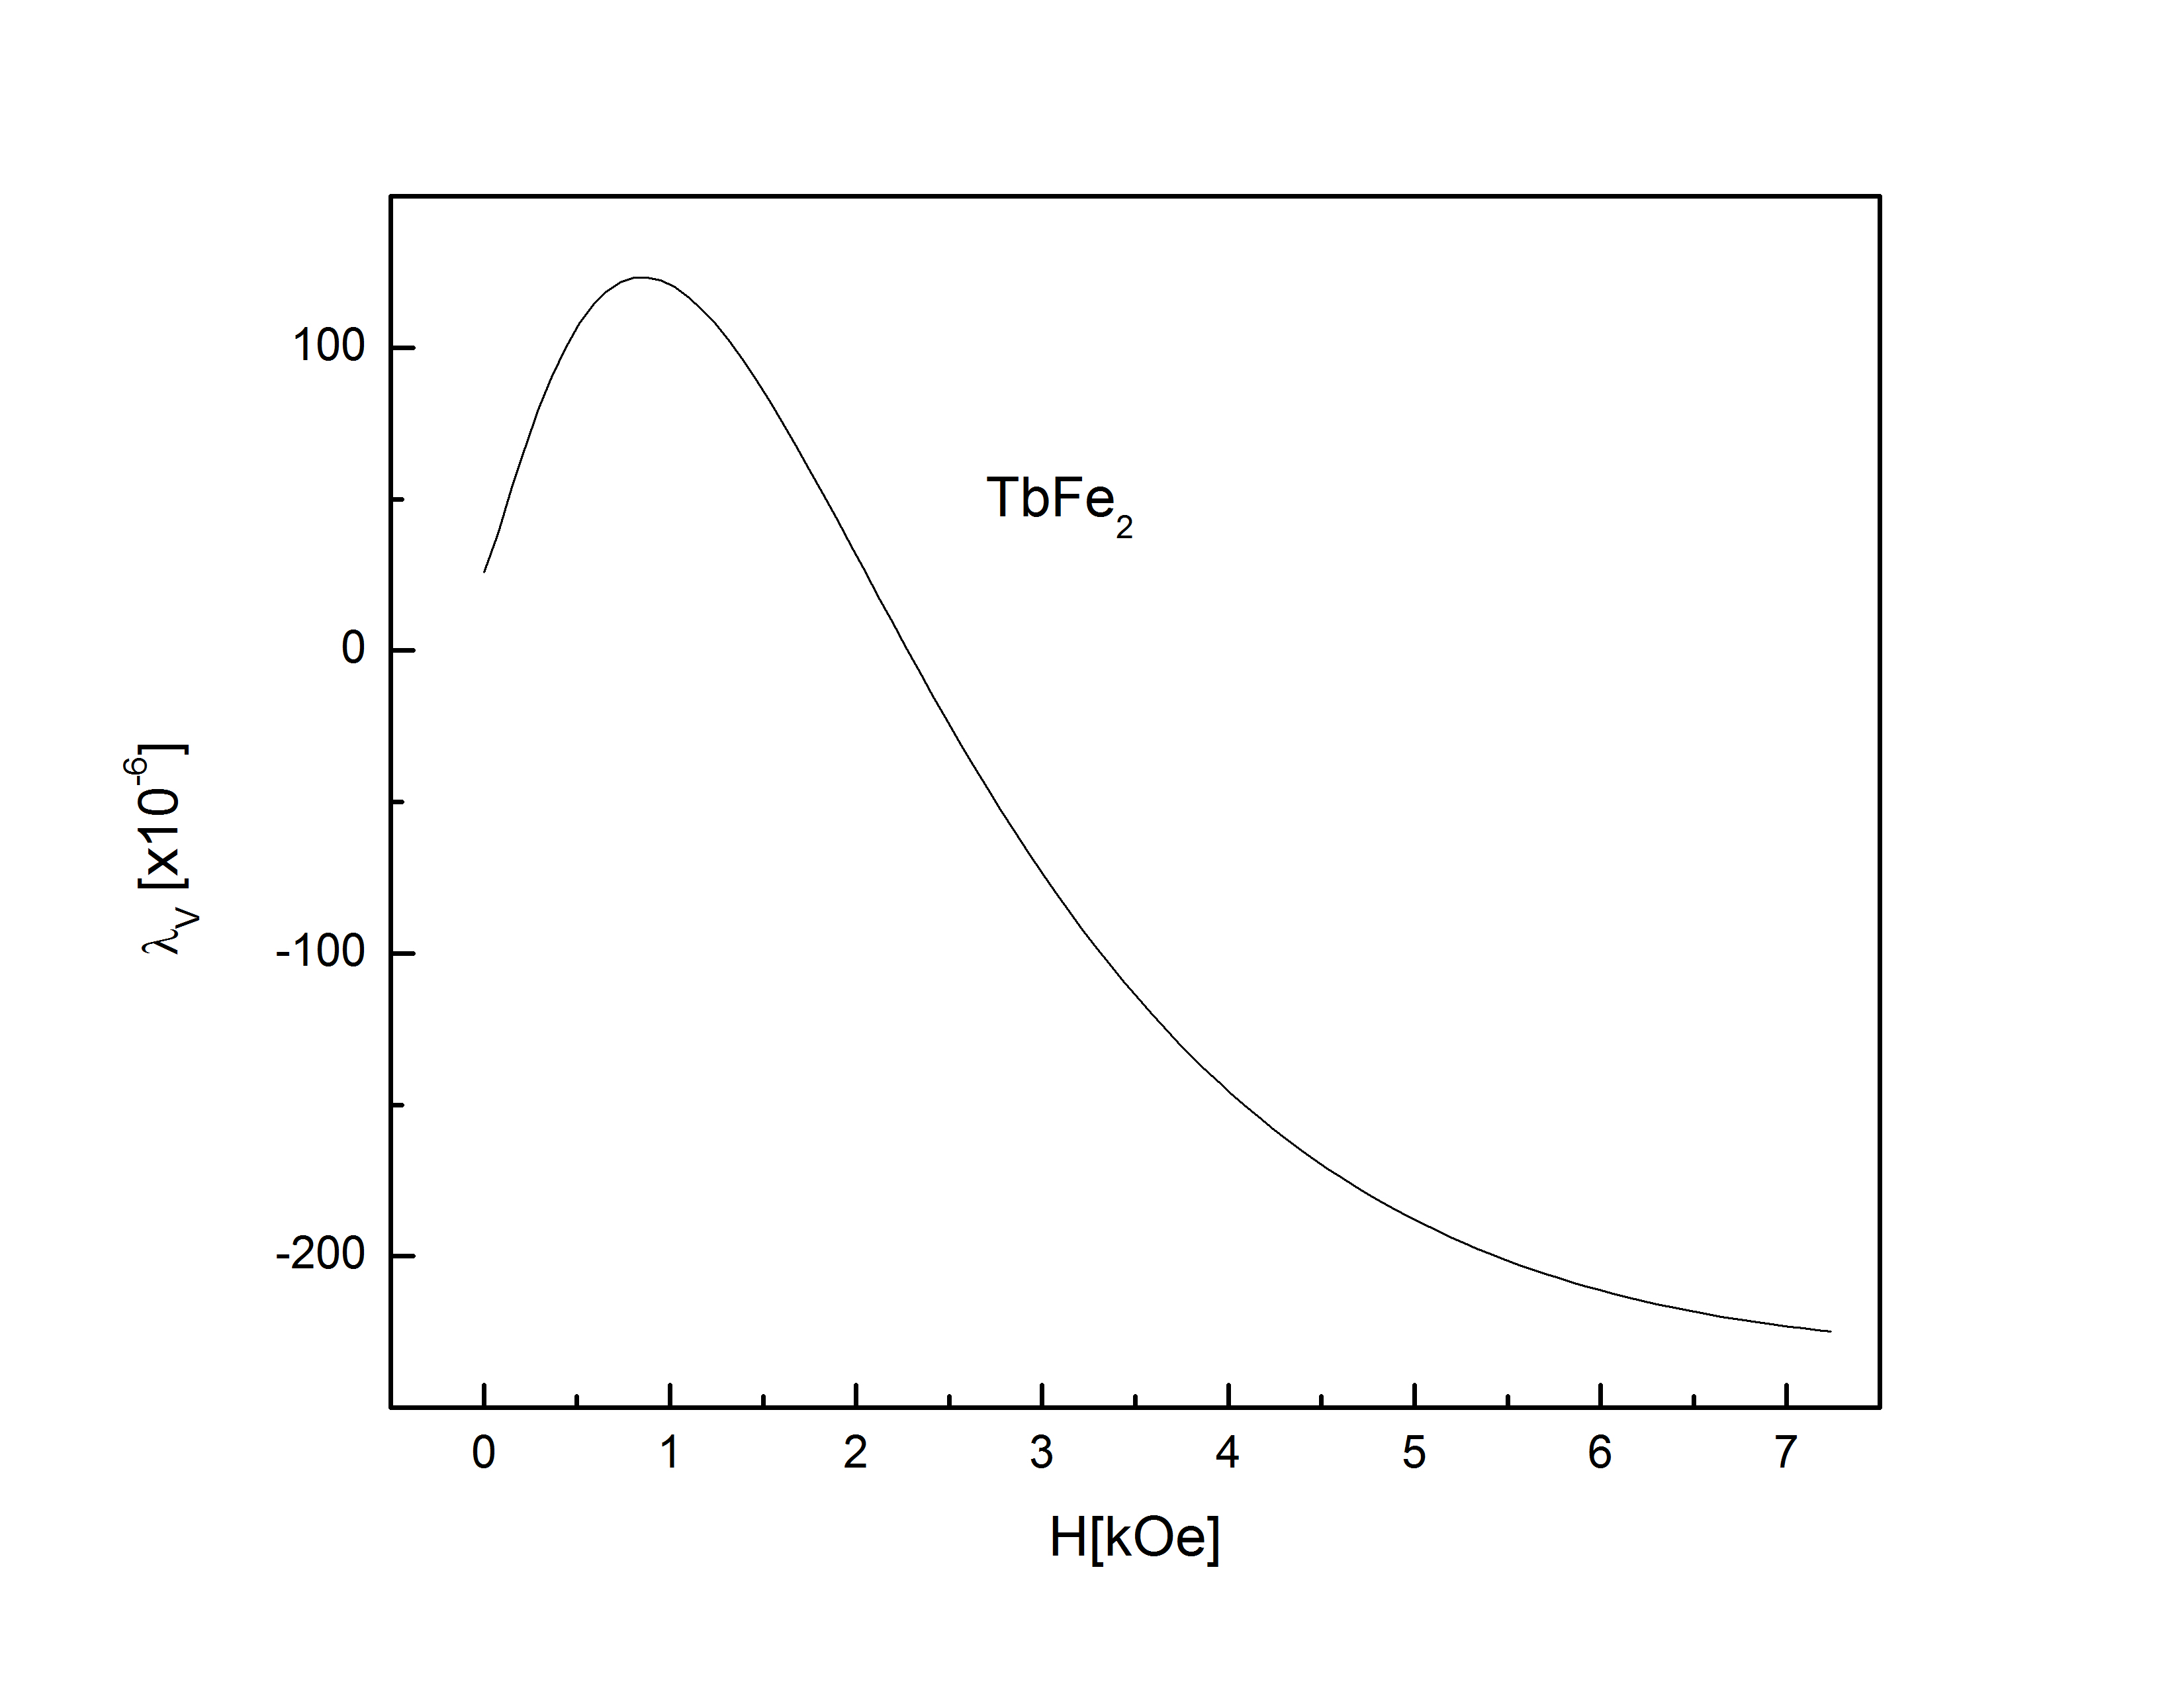
\includegraphics[width =0.9\textwidth]{../img/magneto/TbObjetosc}
    \caption{Wartość magnetostrykcji objetości $\lambda_{V}$ $TbFe_2$}
    \label{TbObjetosc}
\end{figure}


%---------------------------------------Y-------------------------------------


\begin{figure}[h]
    \centering
    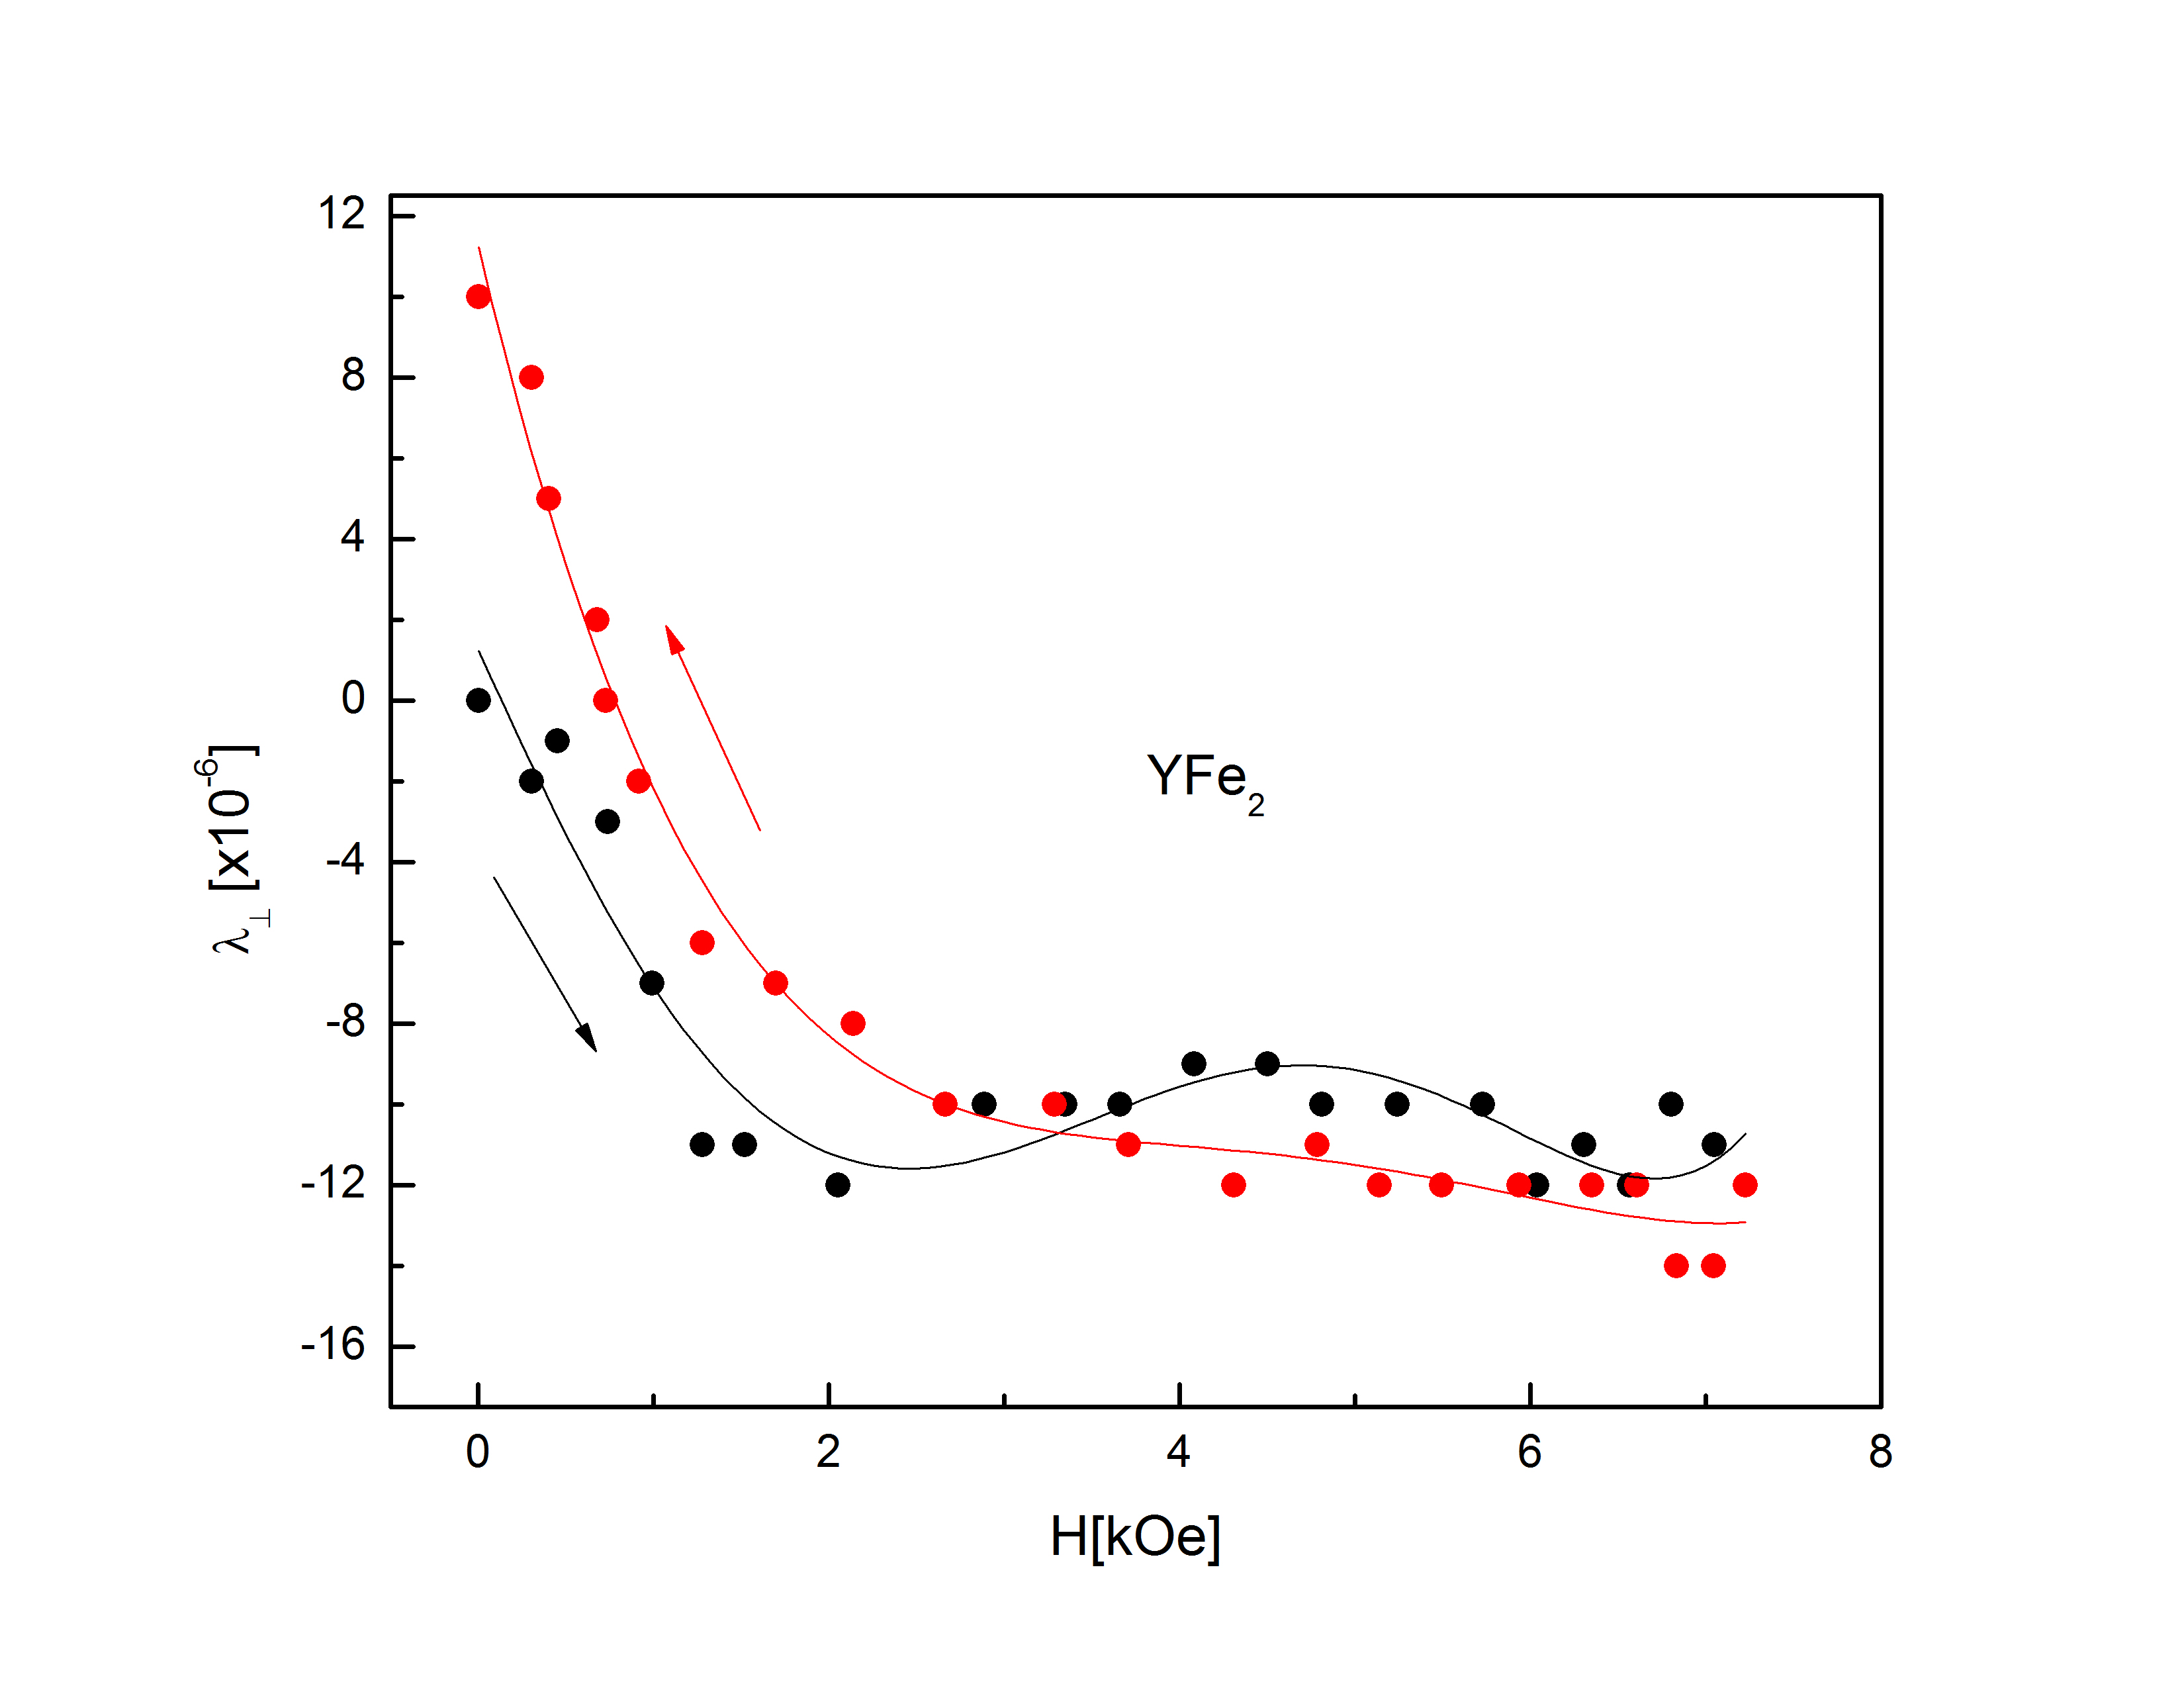
\includegraphics[width =0.9\textwidth]{../img/magneto/Ypoprzeczna}
    \caption{Wartość magnetostrykcji poprzecznej $\lambda_{\perp}$ $YFe_2$}
    \label{Ypoprzeczna}
\end{figure}

\begin{figure}[h]
    \centering
    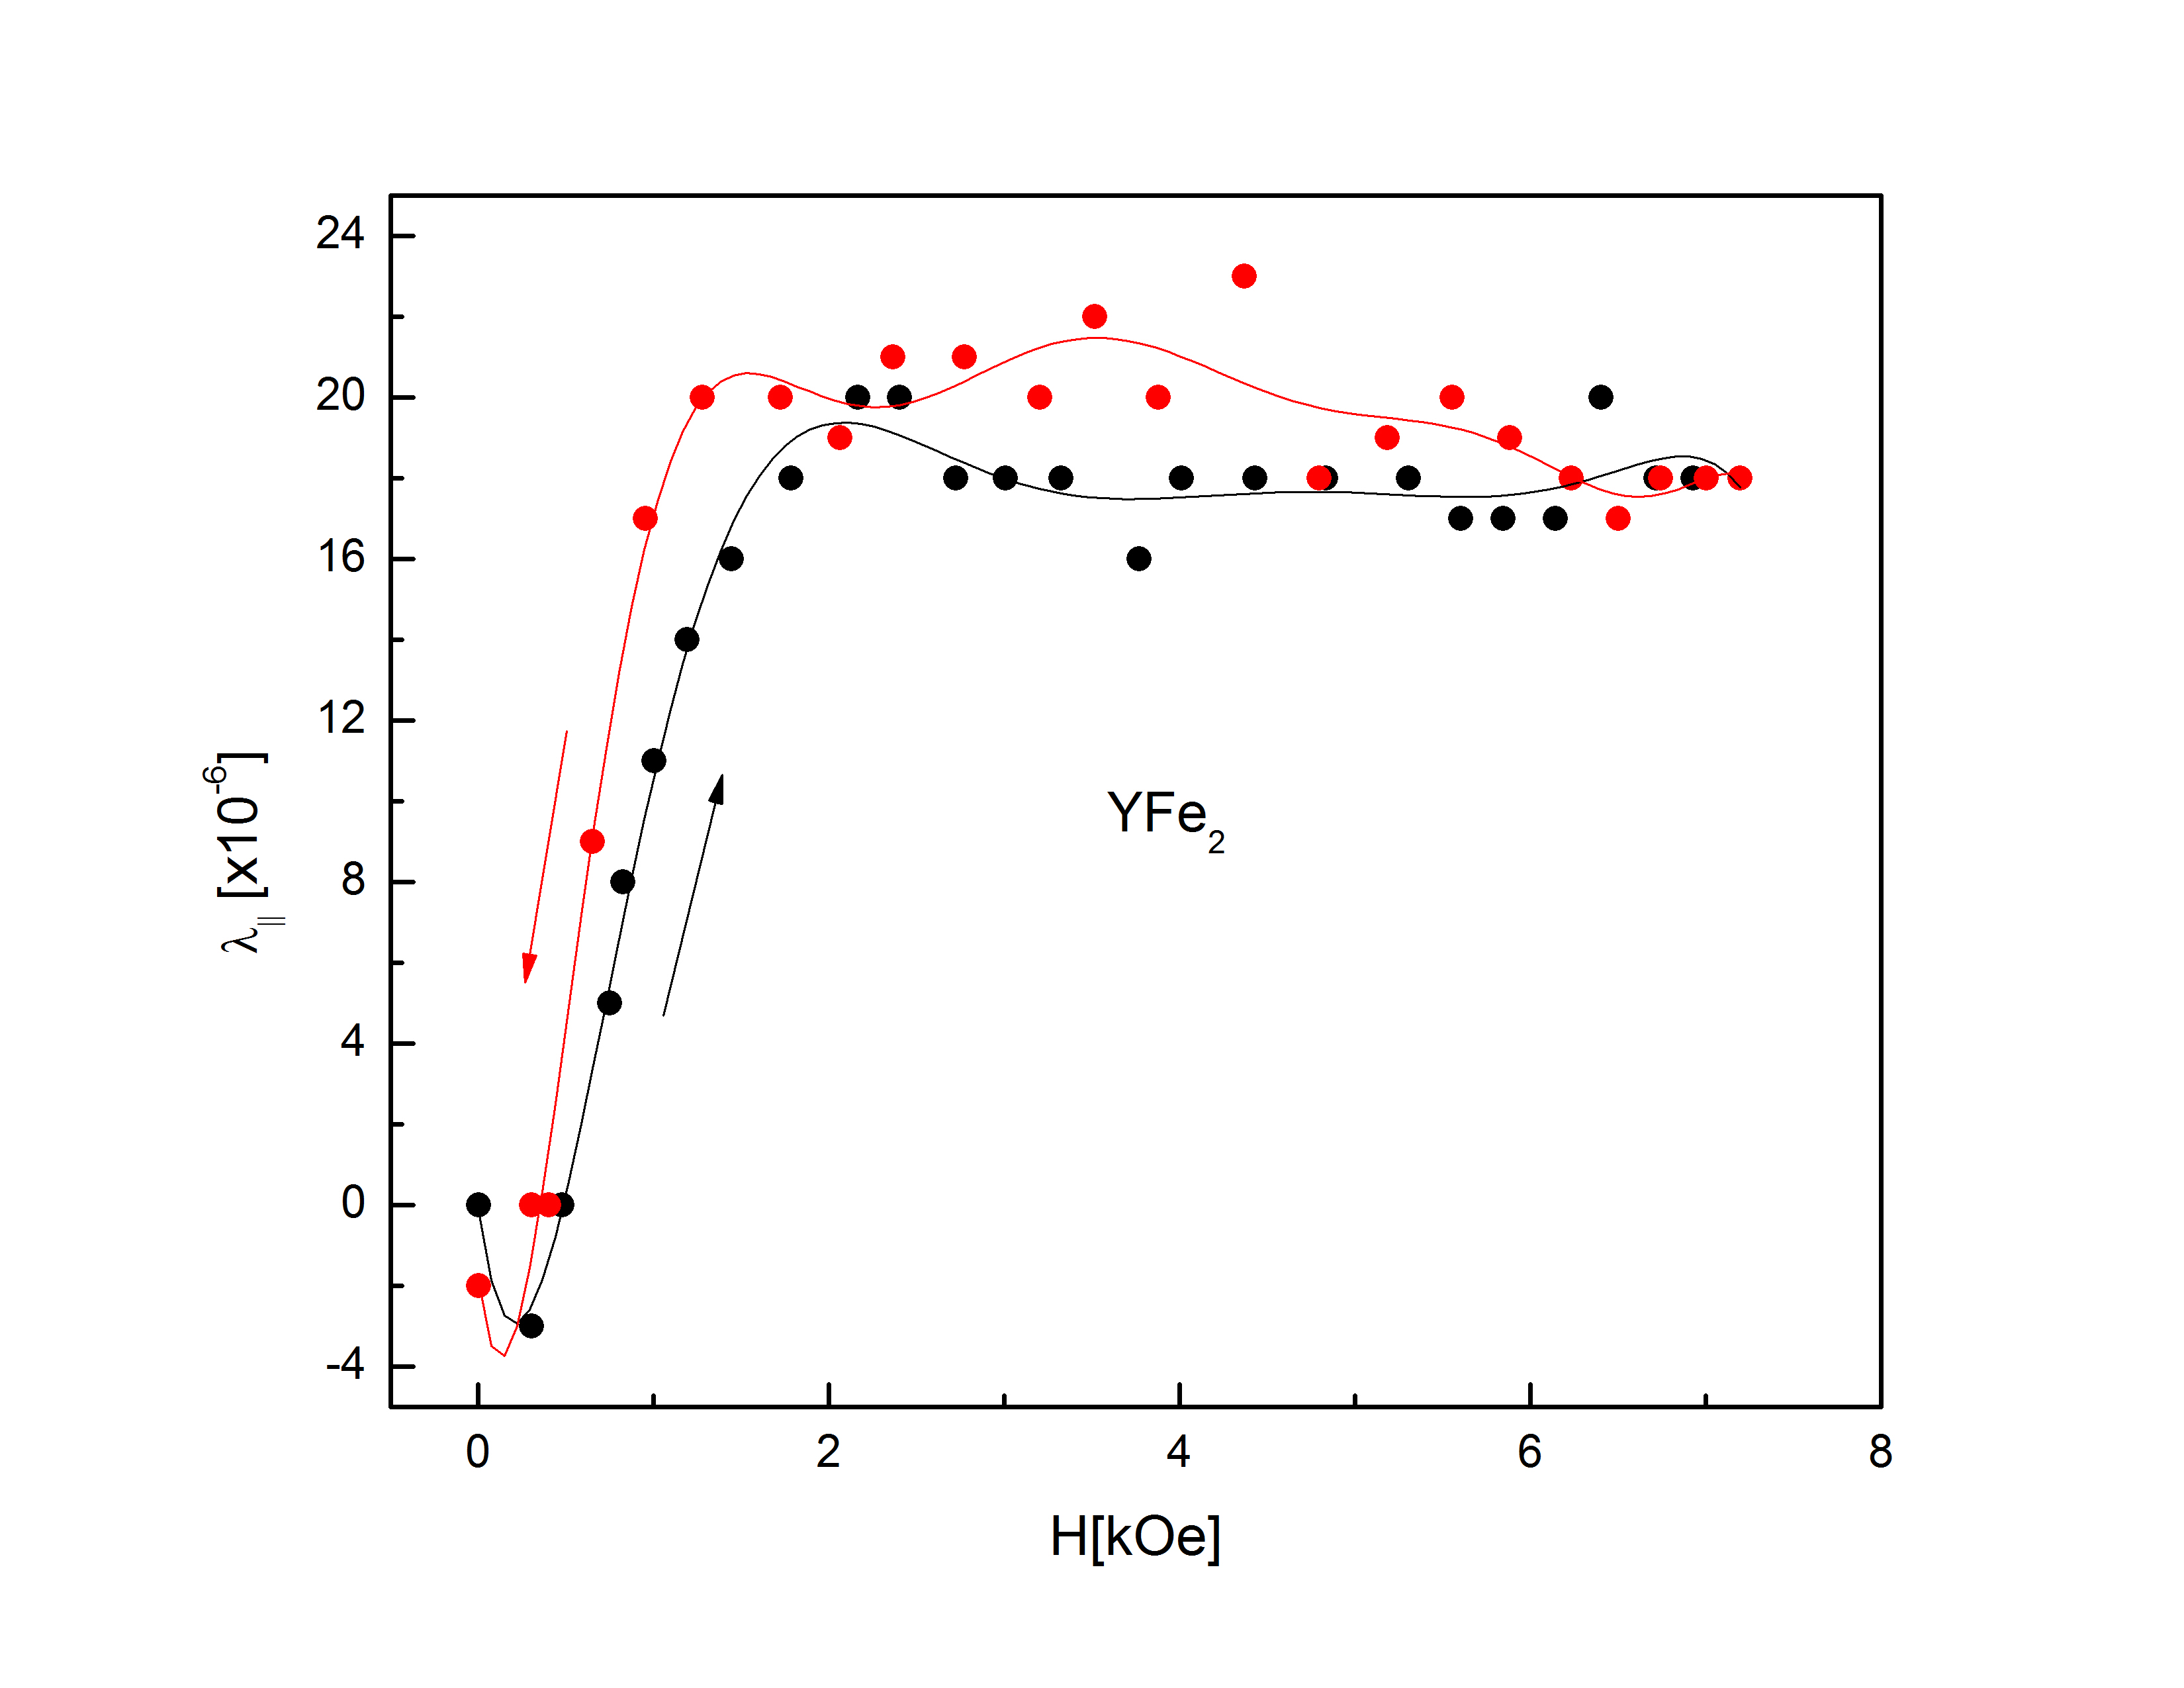
\includegraphics[width =0.9\textwidth]{../img/magneto/Ywzdluzna}
    \caption{Wartość magnetostrykcji wzdłużnej $\lambda_{\parallel}$ $YFe_2$}
    \label{Ywzdluzna}
\end{figure}

\begin{figure}[h]
    \centering
    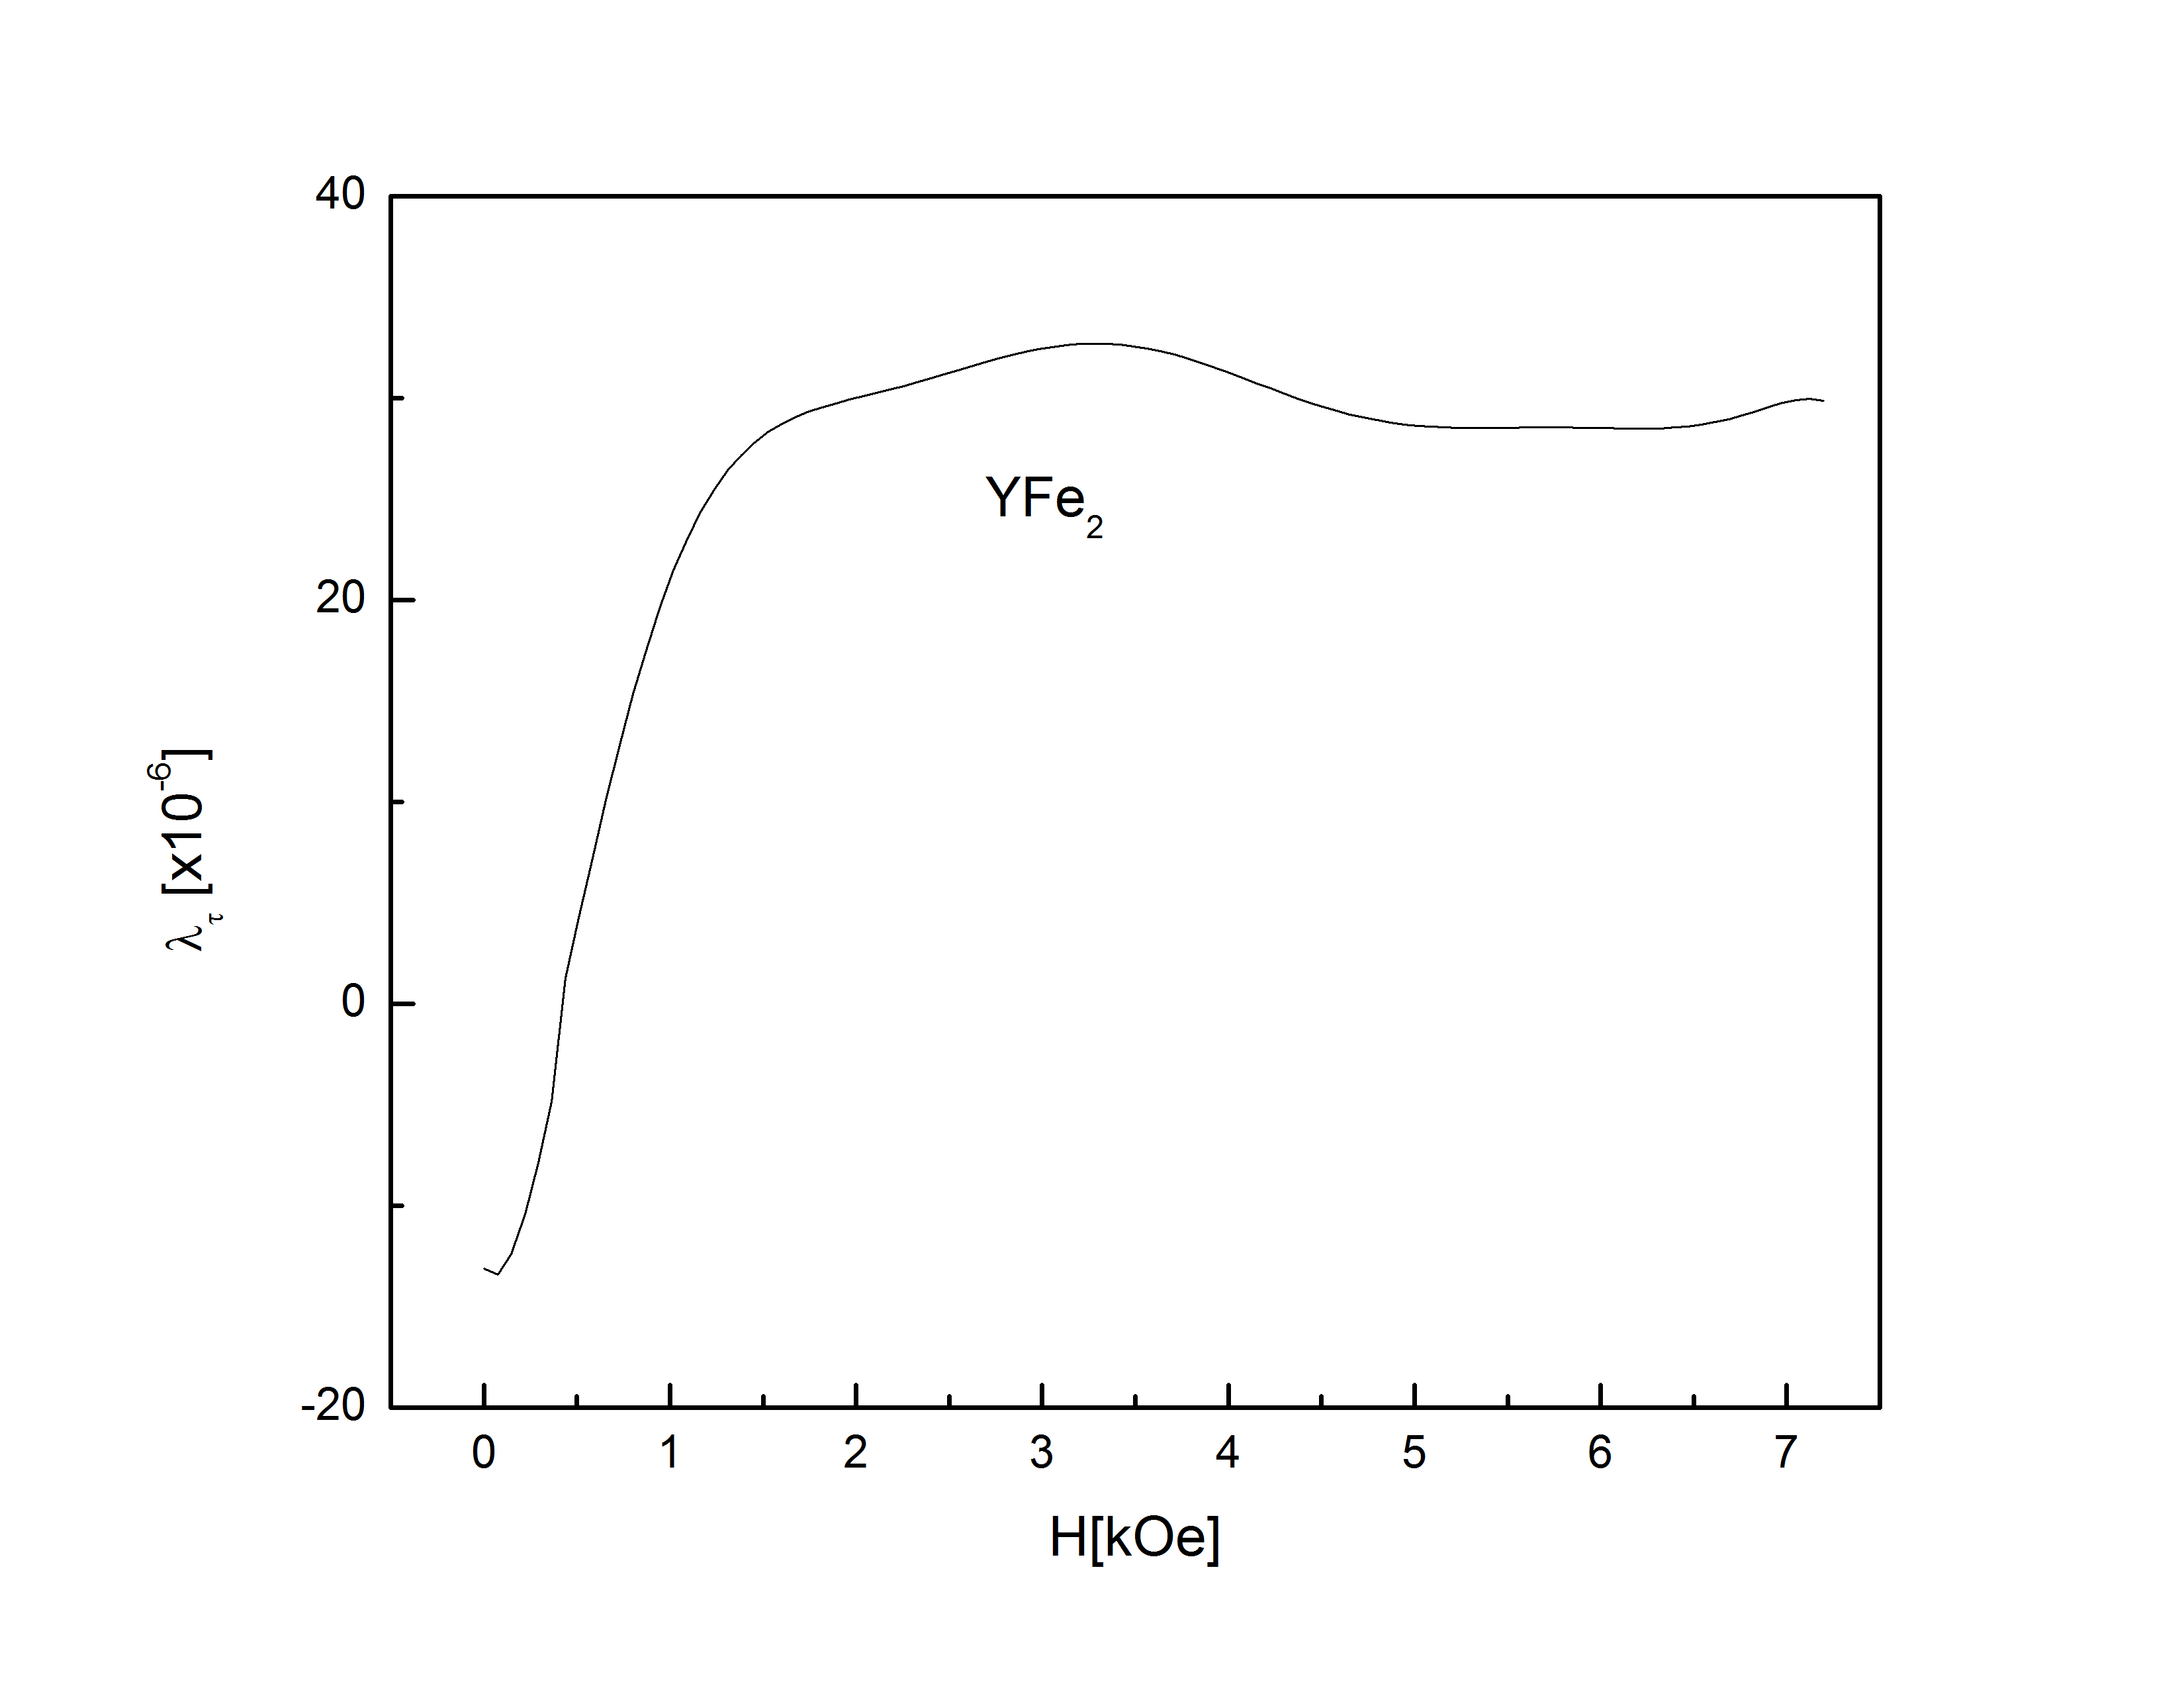
\includegraphics[width =0.9\textwidth]{../img/magneto/YKsztaltu}
    \caption{Wartość magnetostrykcji kształru $\lambda_{\tau}$ $YFe_2$}
    \label{YKsztaltu}
\end{figure}

\begin{figure}[h]
    \centering
    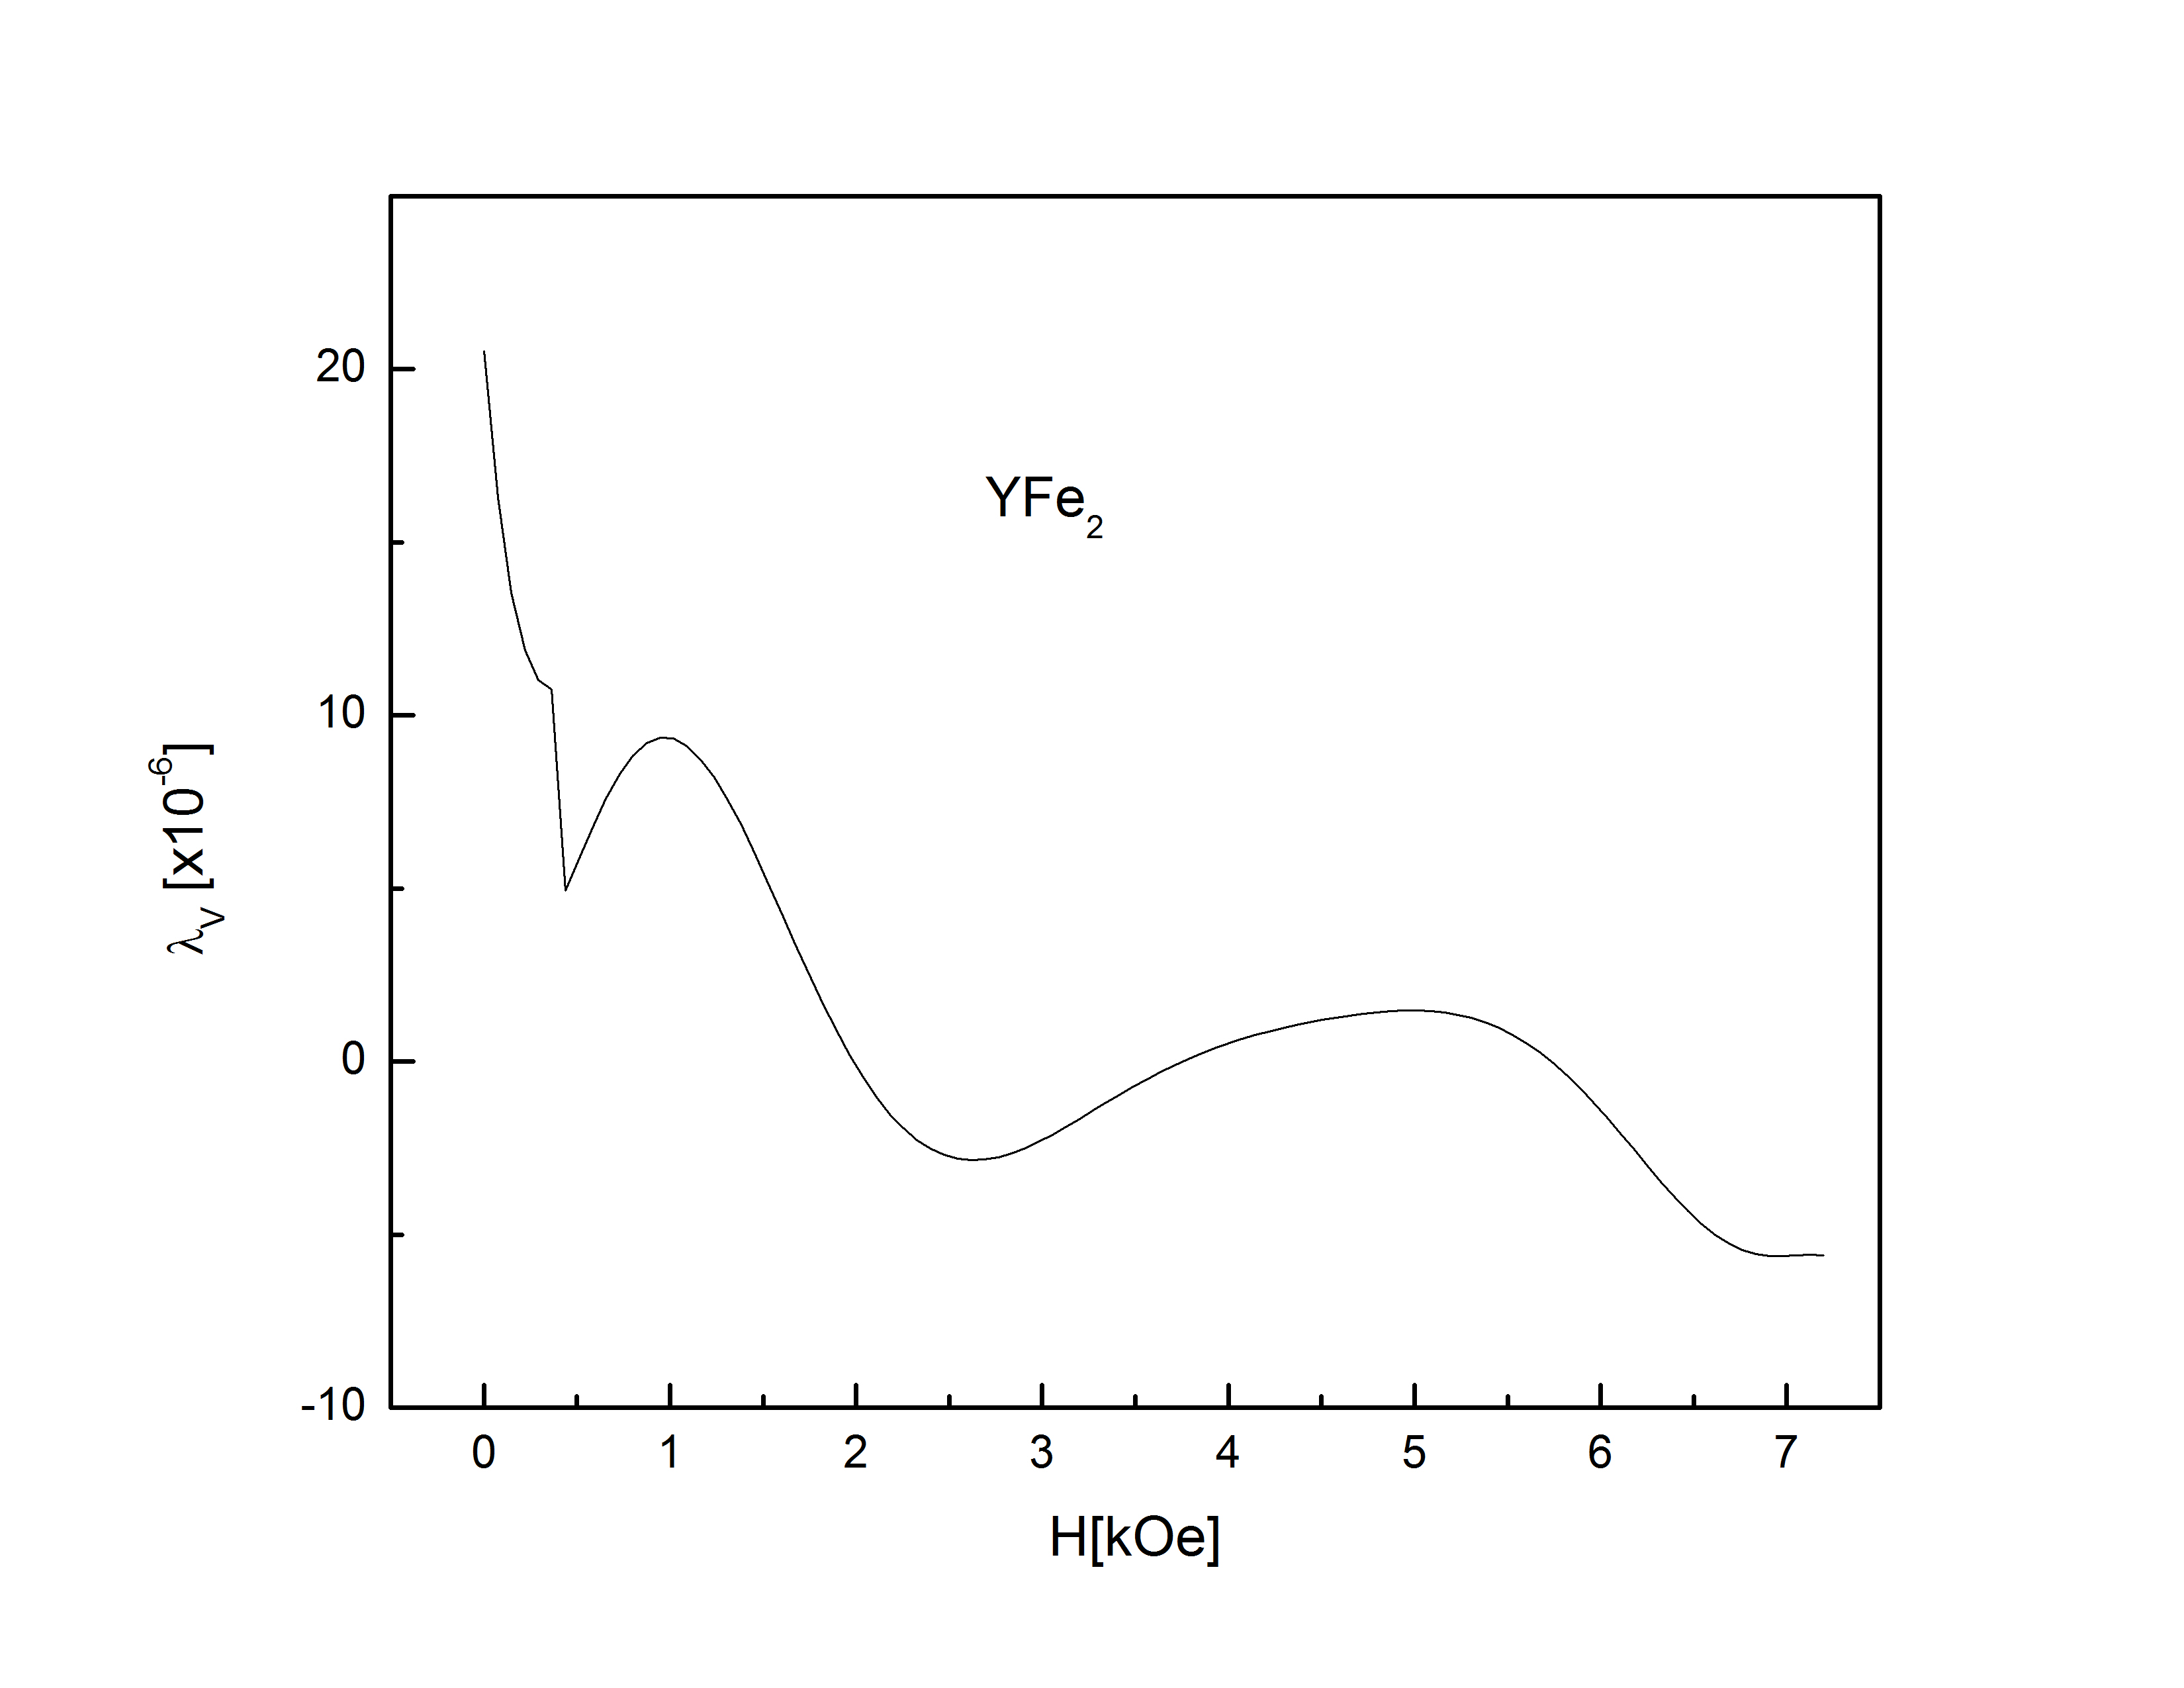
\includegraphics[width =0.9\textwidth]{../img/magneto/YObjetosc}
    \caption{Wartość magnetostrykcji objetości $\lambda_{V}$ $YFe_2$}
    \label{YObjetosc}
\end{figure}


%\newpage

\documentclass[a4paper,12pt]{article}

\usepackage[utf8]{inputenc}
\usepackage[T1]{polski}
\usepackage{helvet}
\usepackage{color}
\usepackage{tabularx}
\usepackage[pdftex]{graphicx}
\usepackage{graphicx}
\usepackage{amsmath}
\usepackage{geometry}
\usepackage{multirow}
\usepackage{indentfirst}
\usepackage{wrapfig}
\usepackage{caption}
\usepackage[titletoc]{appendix}
\usepackage[nottoc]{tocbibind}
\usepackage{pdfpages}
\usepackage{hyperref}
\usepackage{chngcntr}
\usepackage{caption}
\usepackage{rotating}
\usepackage{longtable}



\hypersetup{colorlinks,linkcolor=black,citecolor=blue}
\captionsetup{margin=10pt, font={small,it}, labelfont=bf}
\renewcommand{\figurename}{Rys.}
\renewcommand{\appendixname}{Dodatek}



\numberwithin{equation}{section}
\counterwithin{table}{section}
\counterwithin{figure}{section}

\renewcommand{\thefigure}{\thesection.\arabic{figure}}


\linespread{1.3}
\widowpenalty=500 %usuwanie wdów
\clubpenalty=500 %usuwanie bękartów i sierot
\newcommand{\nit}[1]{\textnormal{#1}}

%\geometry{hmargin={2cm, 2cm}, height=10.0in}

\begin{document}
\renewcommand{\thetable}{\arabic{section}.\arabic{table}}

%-----------------------------------------------------------------------------------------
%-------------------------Wyniki pomiaru oporności-------------------------------------
%-----------------------------------------------------------------------------------------

\subsection{Wyniki pomiarów oporności elektrycznej}

Dla zmierzonych wartości oporności właściwej $\rho$ dopasowano zgodnie ze wzorami MIEJSCE NA REFLINKI DO WZORÓW
dla pomiarów niskotemperaturowcyh wielomian piątego stopnia o współczynnikach $a_3$ i $a_4$ równymi zero, oraz prostą dla
pomiarów wysokotemperaturowych. Otrzymane współczynniki posłużyły do wyznaczenia wartości parametrów  $R_t$ oraz
$\Theta$, które posłużyły do wyznaczenia wartości oporności $\rho_0$, $\rho_f$(T) i $\rho_m$(T)



%-----------------------------------------Dy-------------------------------------------------


\begin{figure}[ht]
    \centering
    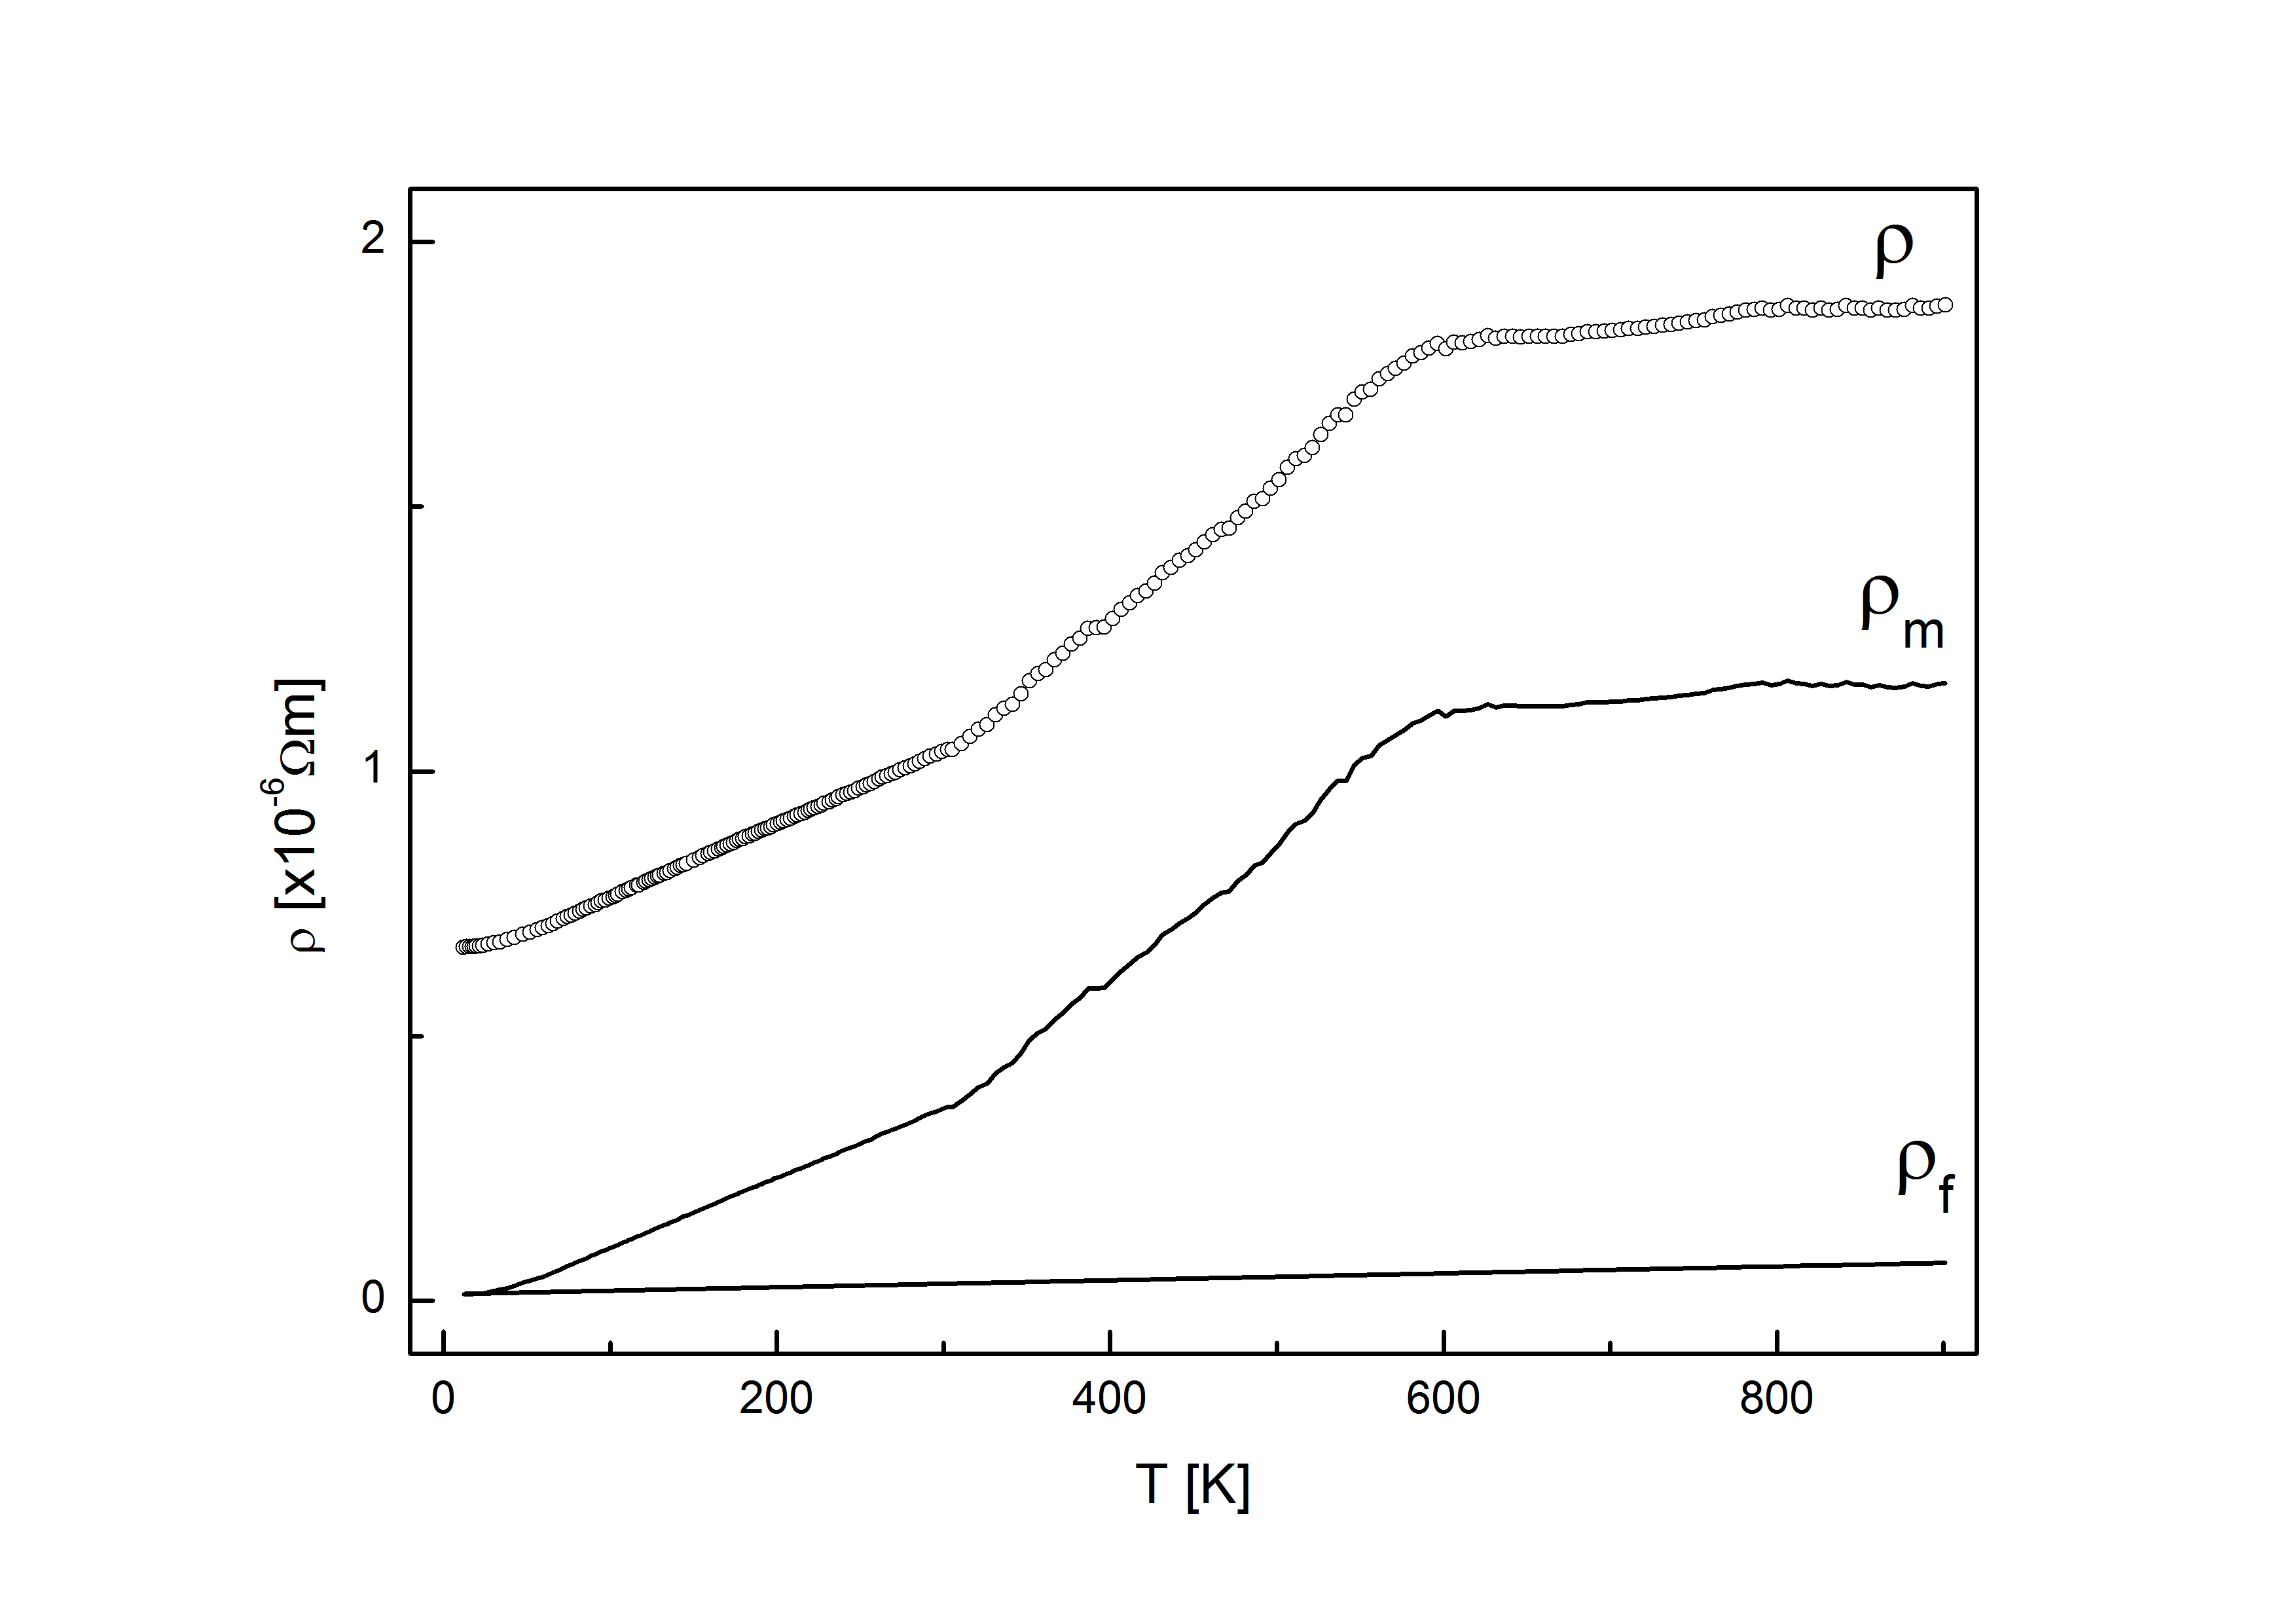
\includegraphics[width =0.85\textwidth]{../img/opor/skladoweDy}
    \caption{Zależność oporności właściwej $\rho$, oporności $\rho_f$ i $\rho_m$ dla $DyFe_2$}
    \label{skladoweDy}
\end{figure}

\begin{figure}[ht]
    \centering
    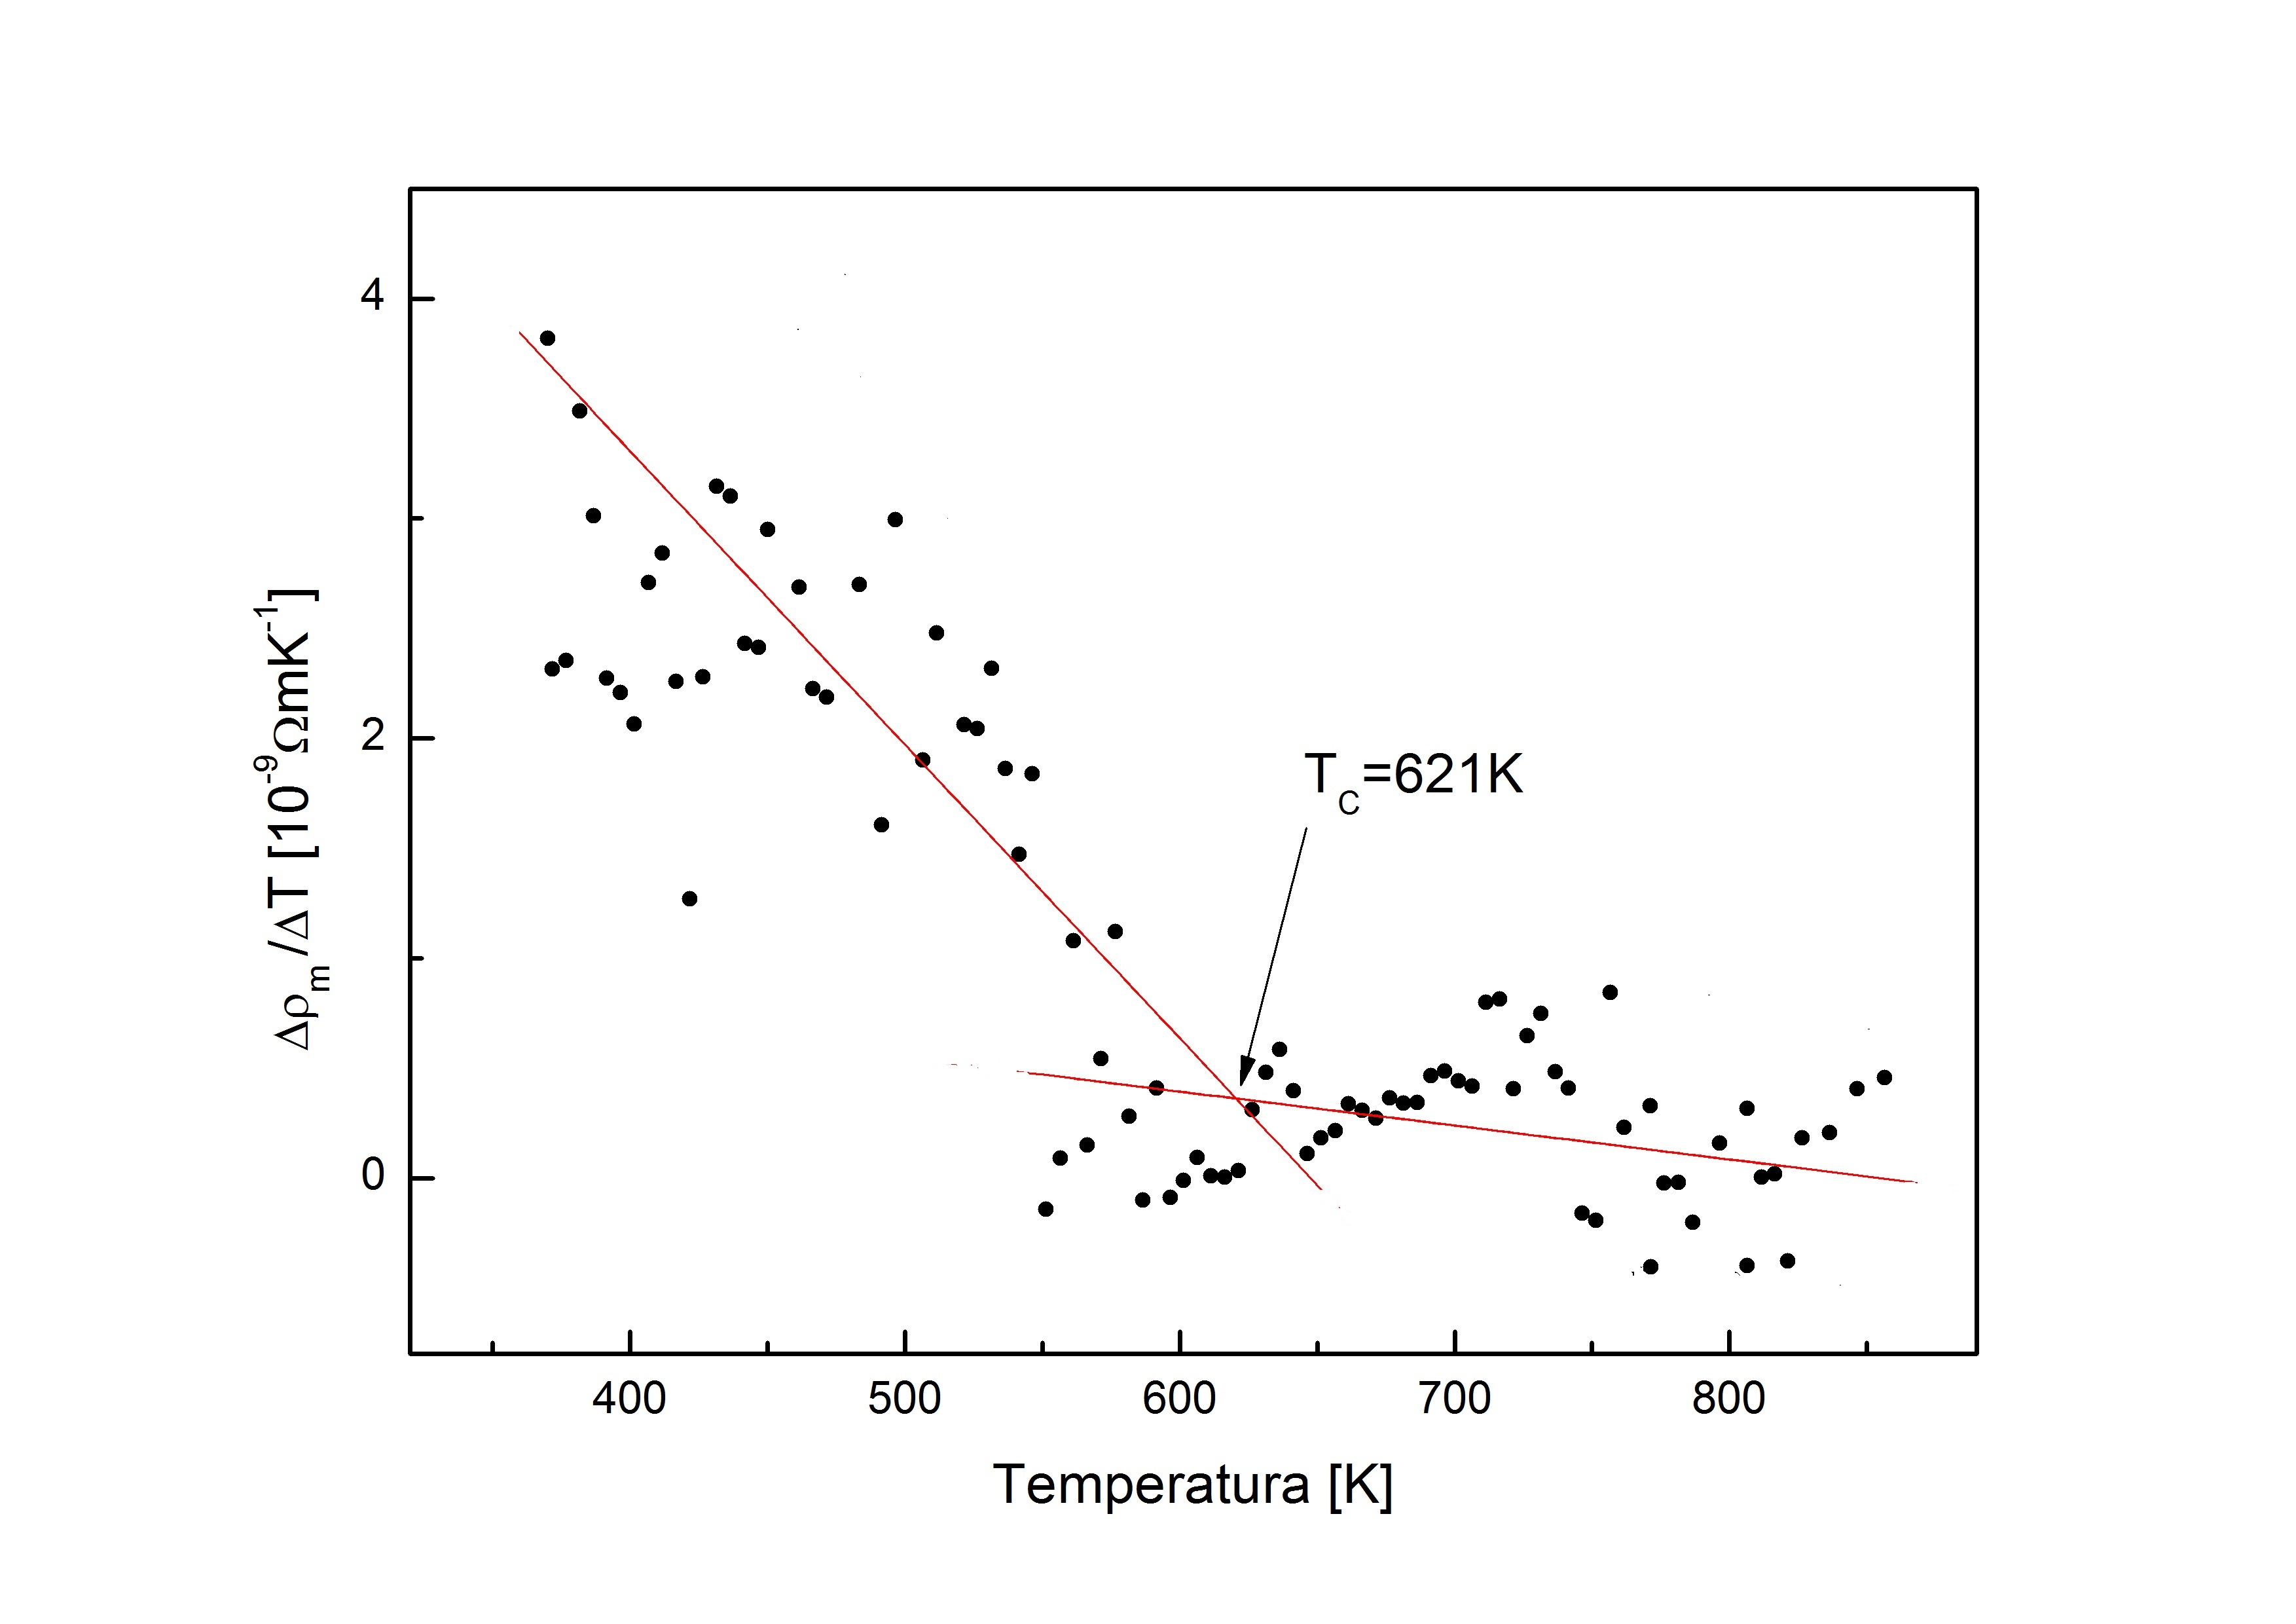
\includegraphics[width =0.8\textwidth]{../img/opor/pochodnaDy}
    \caption{Zależność $\frac{\Delta\rho_m(T)}{\Delta T}$ wraz z wyznaczoną temperaturą Curie $T_C$ dla $DyFe_2$}
    \label{skladoweDy}
\end{figure}

%-----------------------------------------Gd-------------------------------------------------


\begin{figure}[ht]
    \centering
    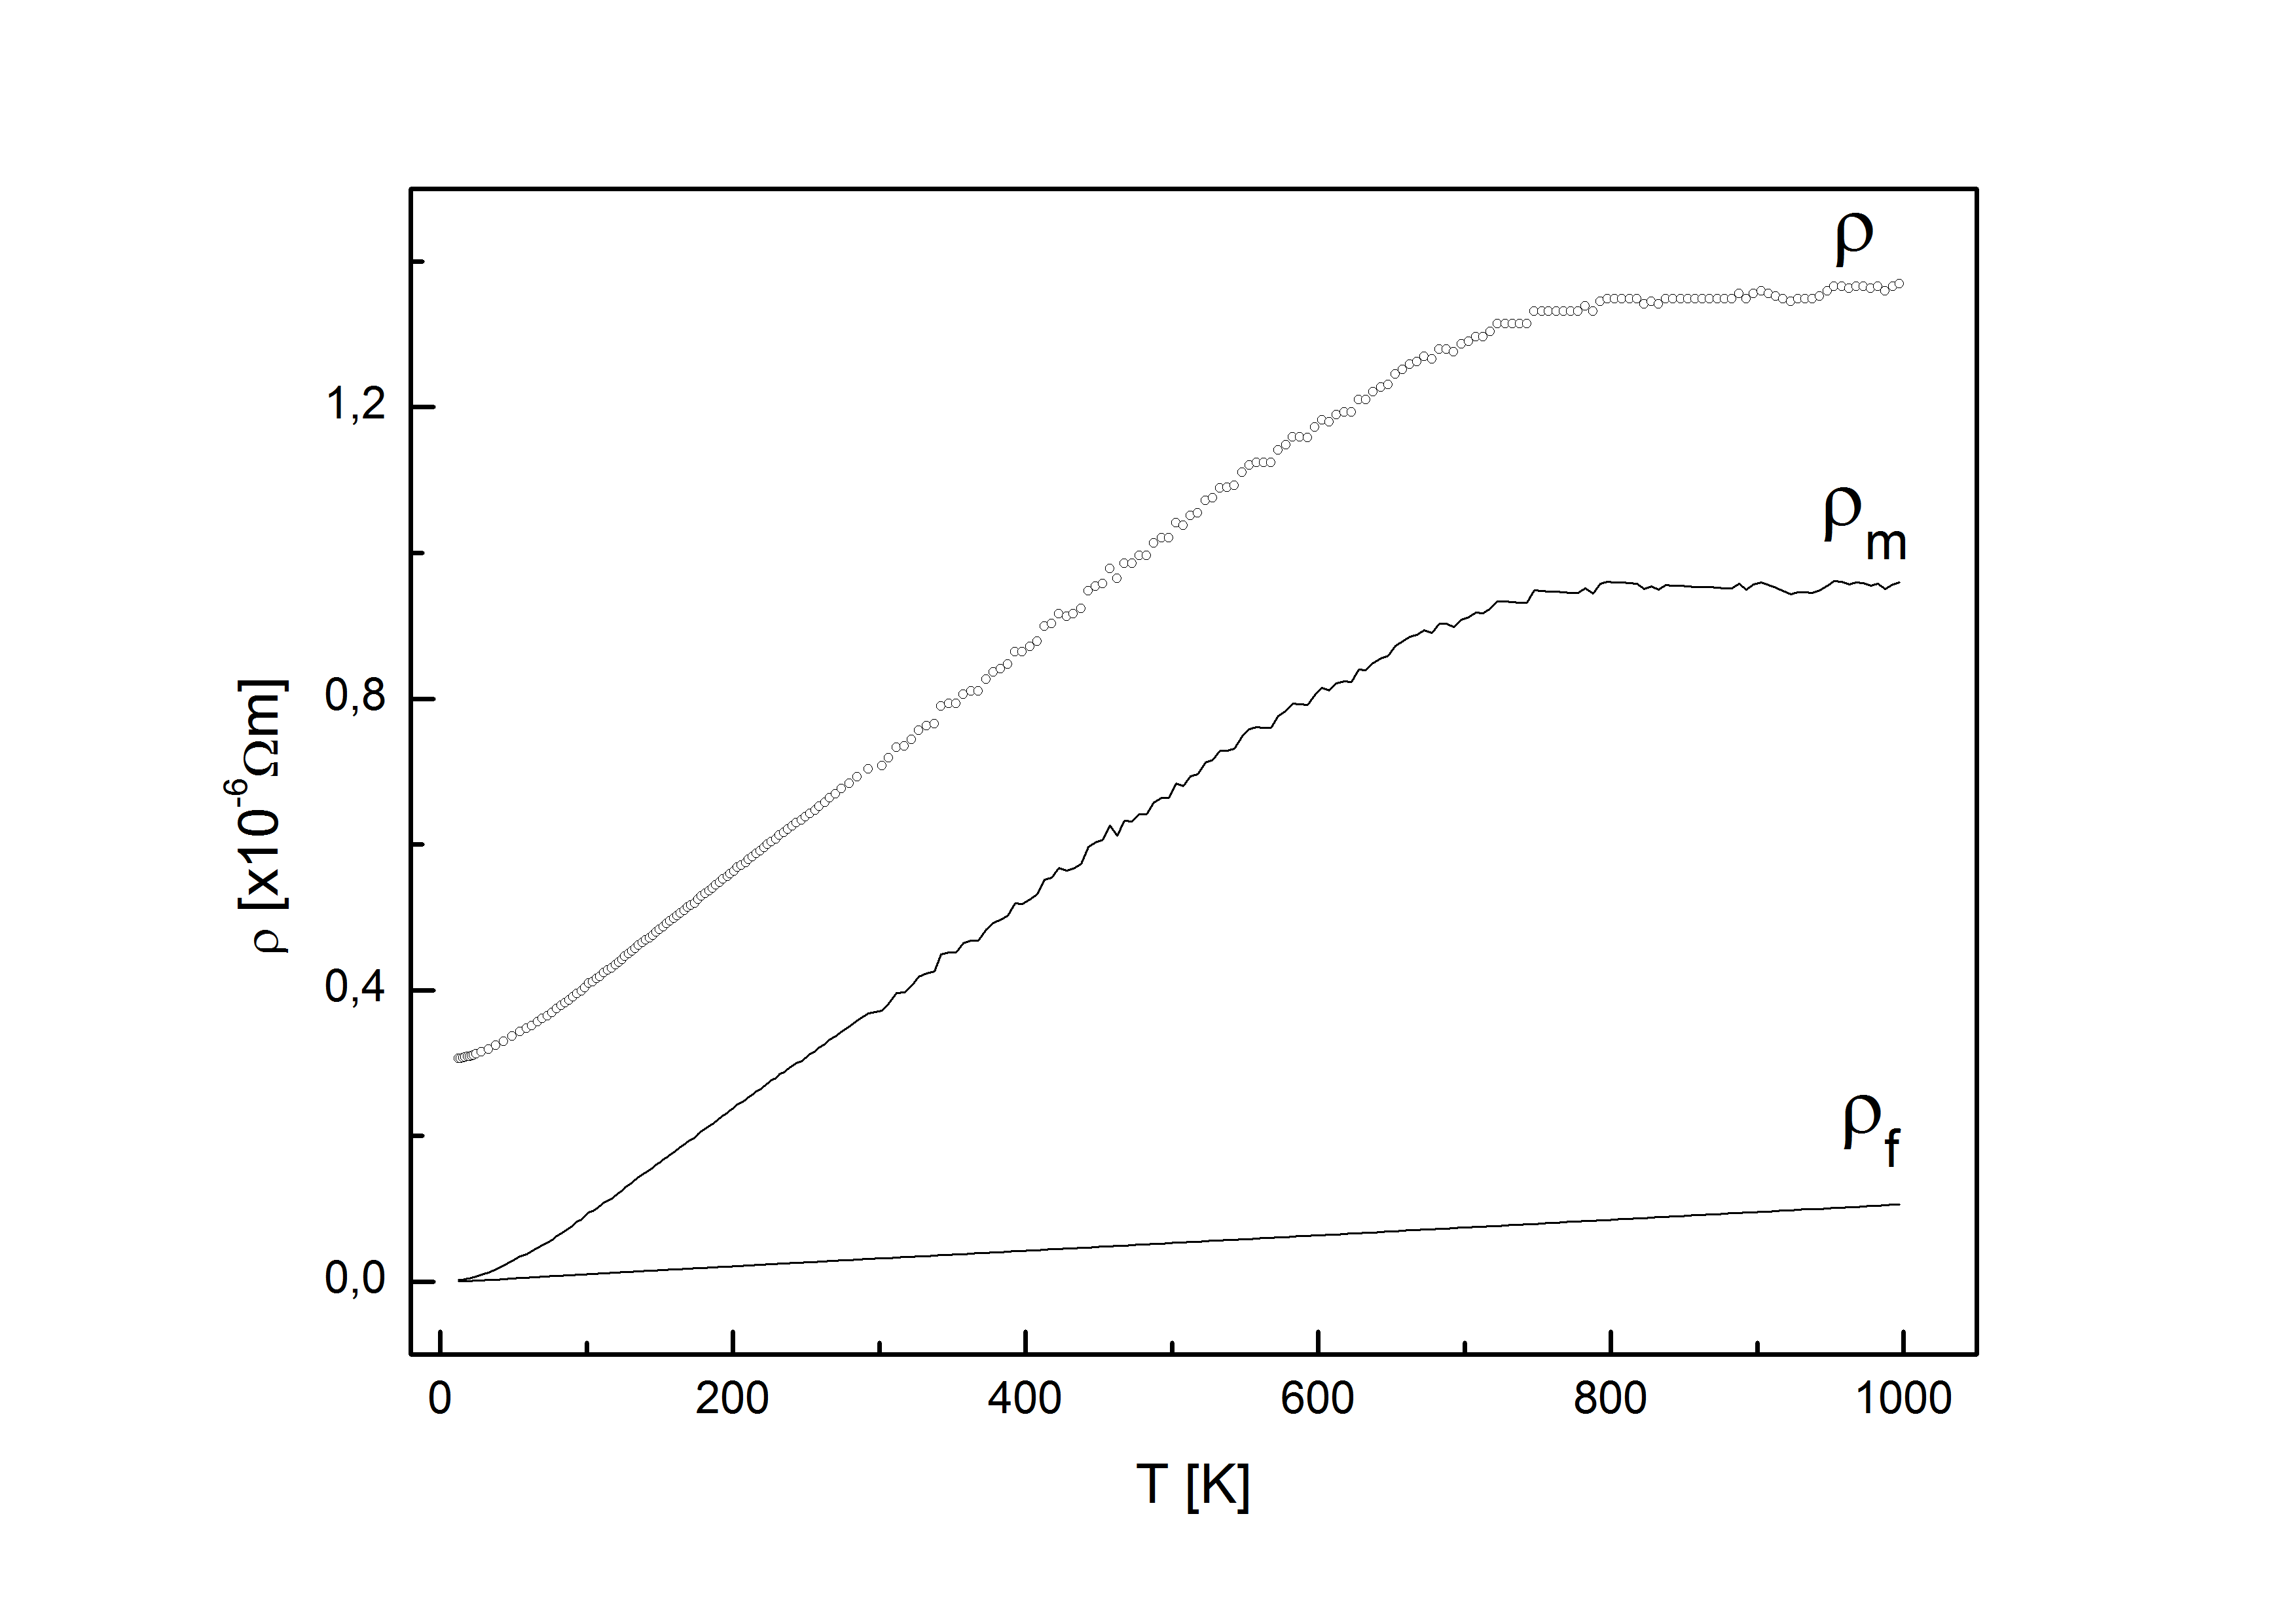
\includegraphics[width =0.8\textwidth]{../img/opor/skladoweGd}
    \caption{Zależność oporności właściwej $\rho$, oporności $\rho_f$ i $\rho_m$ dla $GdFe_2$}
    \label{skladoweGd}
\end{figure}

\begin{figure}[ht]
    \centering
    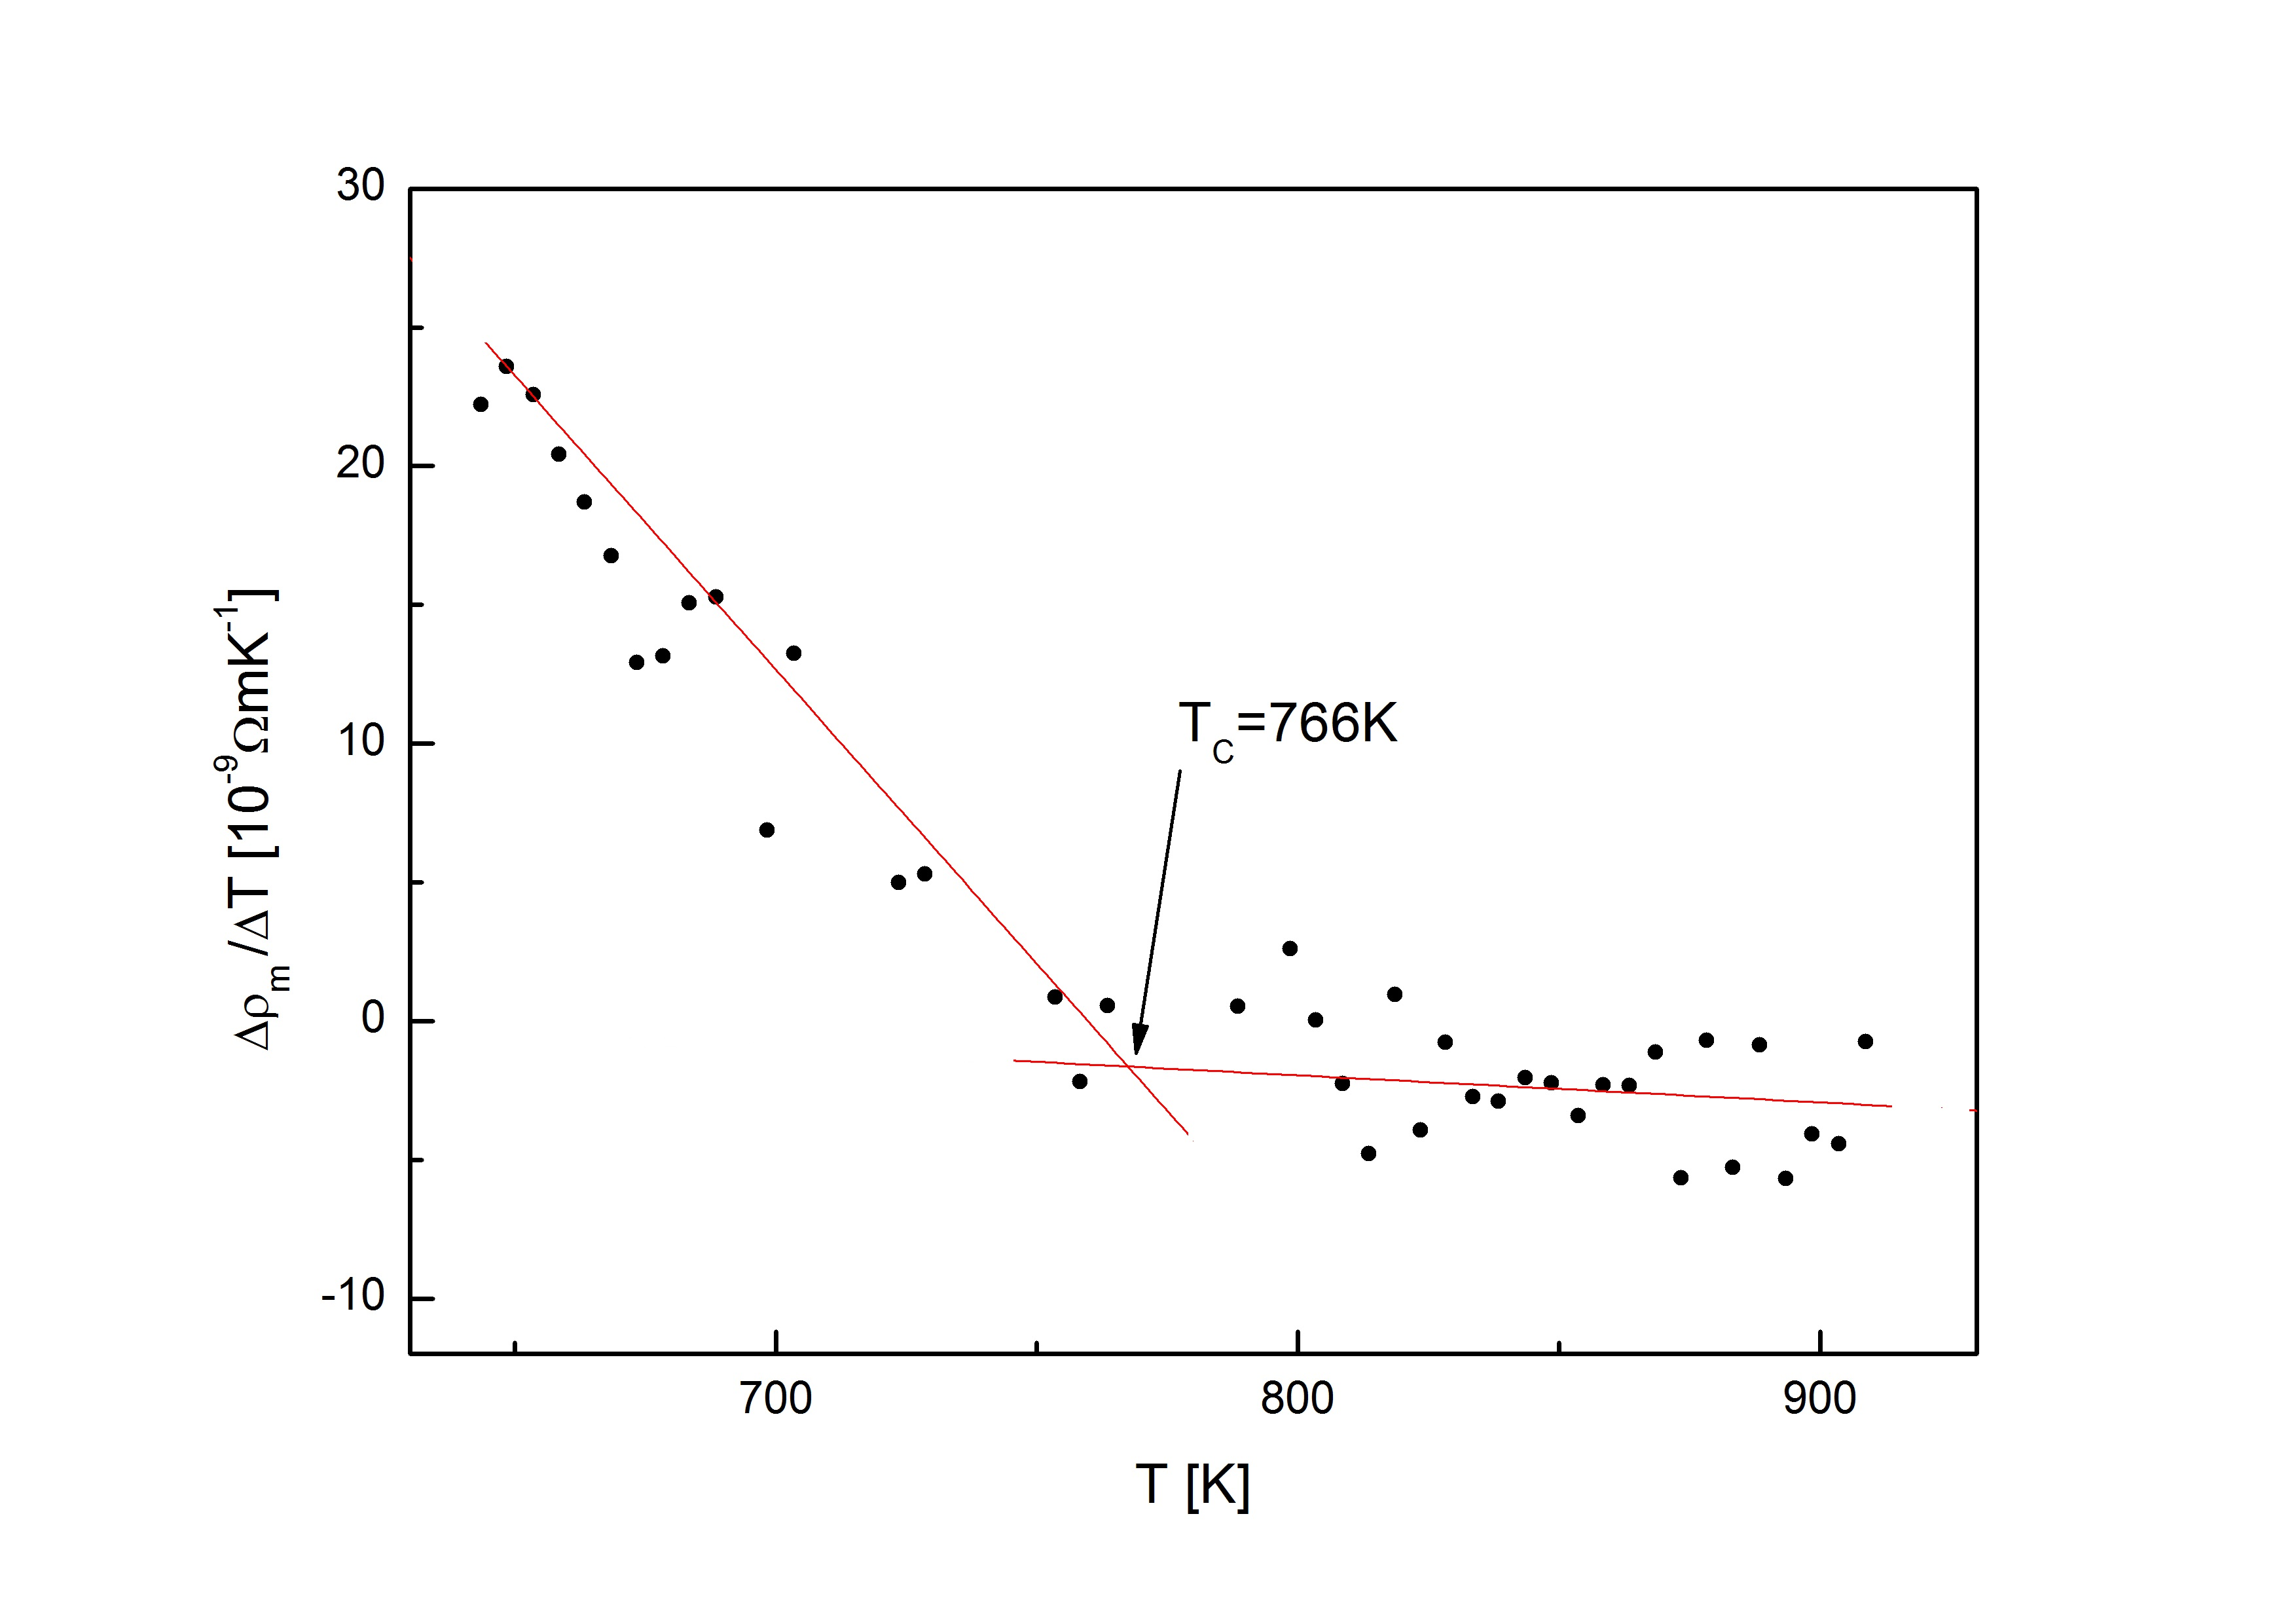
\includegraphics[width =0.8\textwidth]{../img/opor/pochodnaGd}
    \caption{Zależność $\frac{\Delta\rho_m(T)}{\Delta T}$ wraz z wyznaczoną temperaturą Curie $T_C$ dla $GdFe_2$}
    \label{skladoweGd}
\end{figure}


%-----------------------------------------Ho-------------------------------------------------


\begin{figure}[ht]
    \centering
    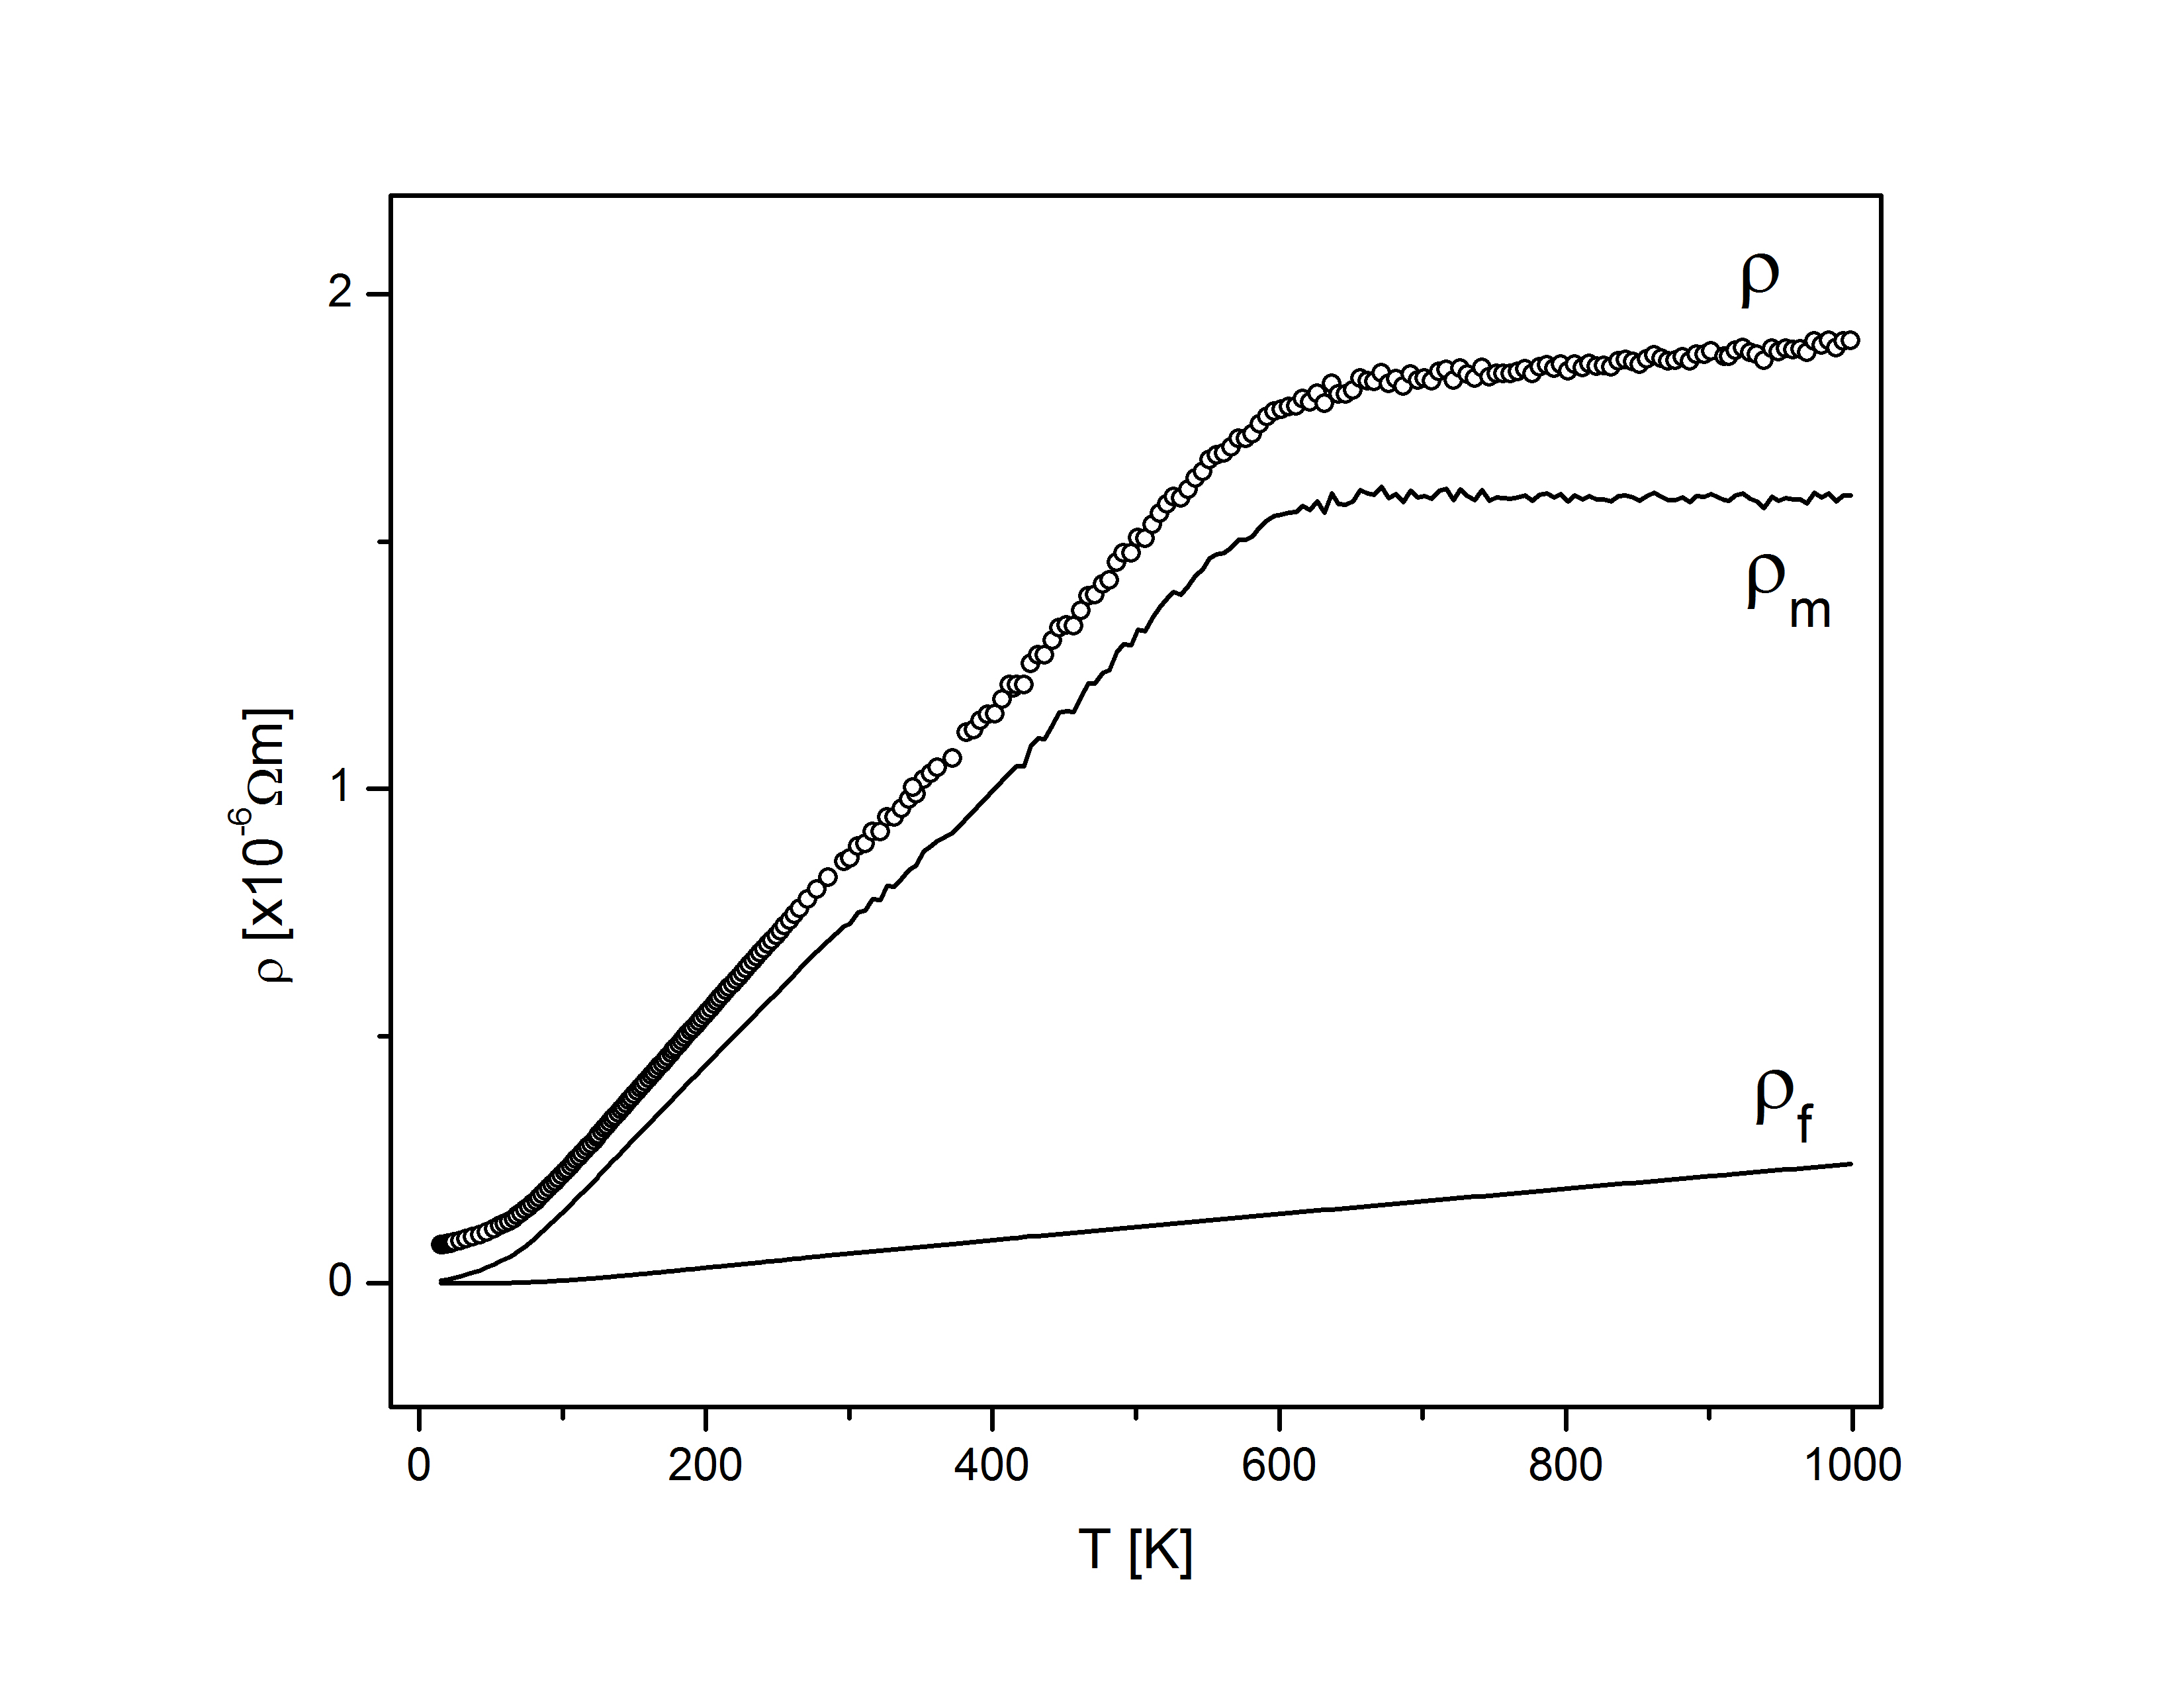
\includegraphics[width =0.8\textwidth]{../img/opor/skladoweHo}
    \caption{Zależność oporności właściwej $\rho$, oporności $\rho_f$ i $\rho_m$ dla $HoFe_2$}
    \label{skladoweHo}
\end{figure}

\begin{figure}[ht]
    \centering
    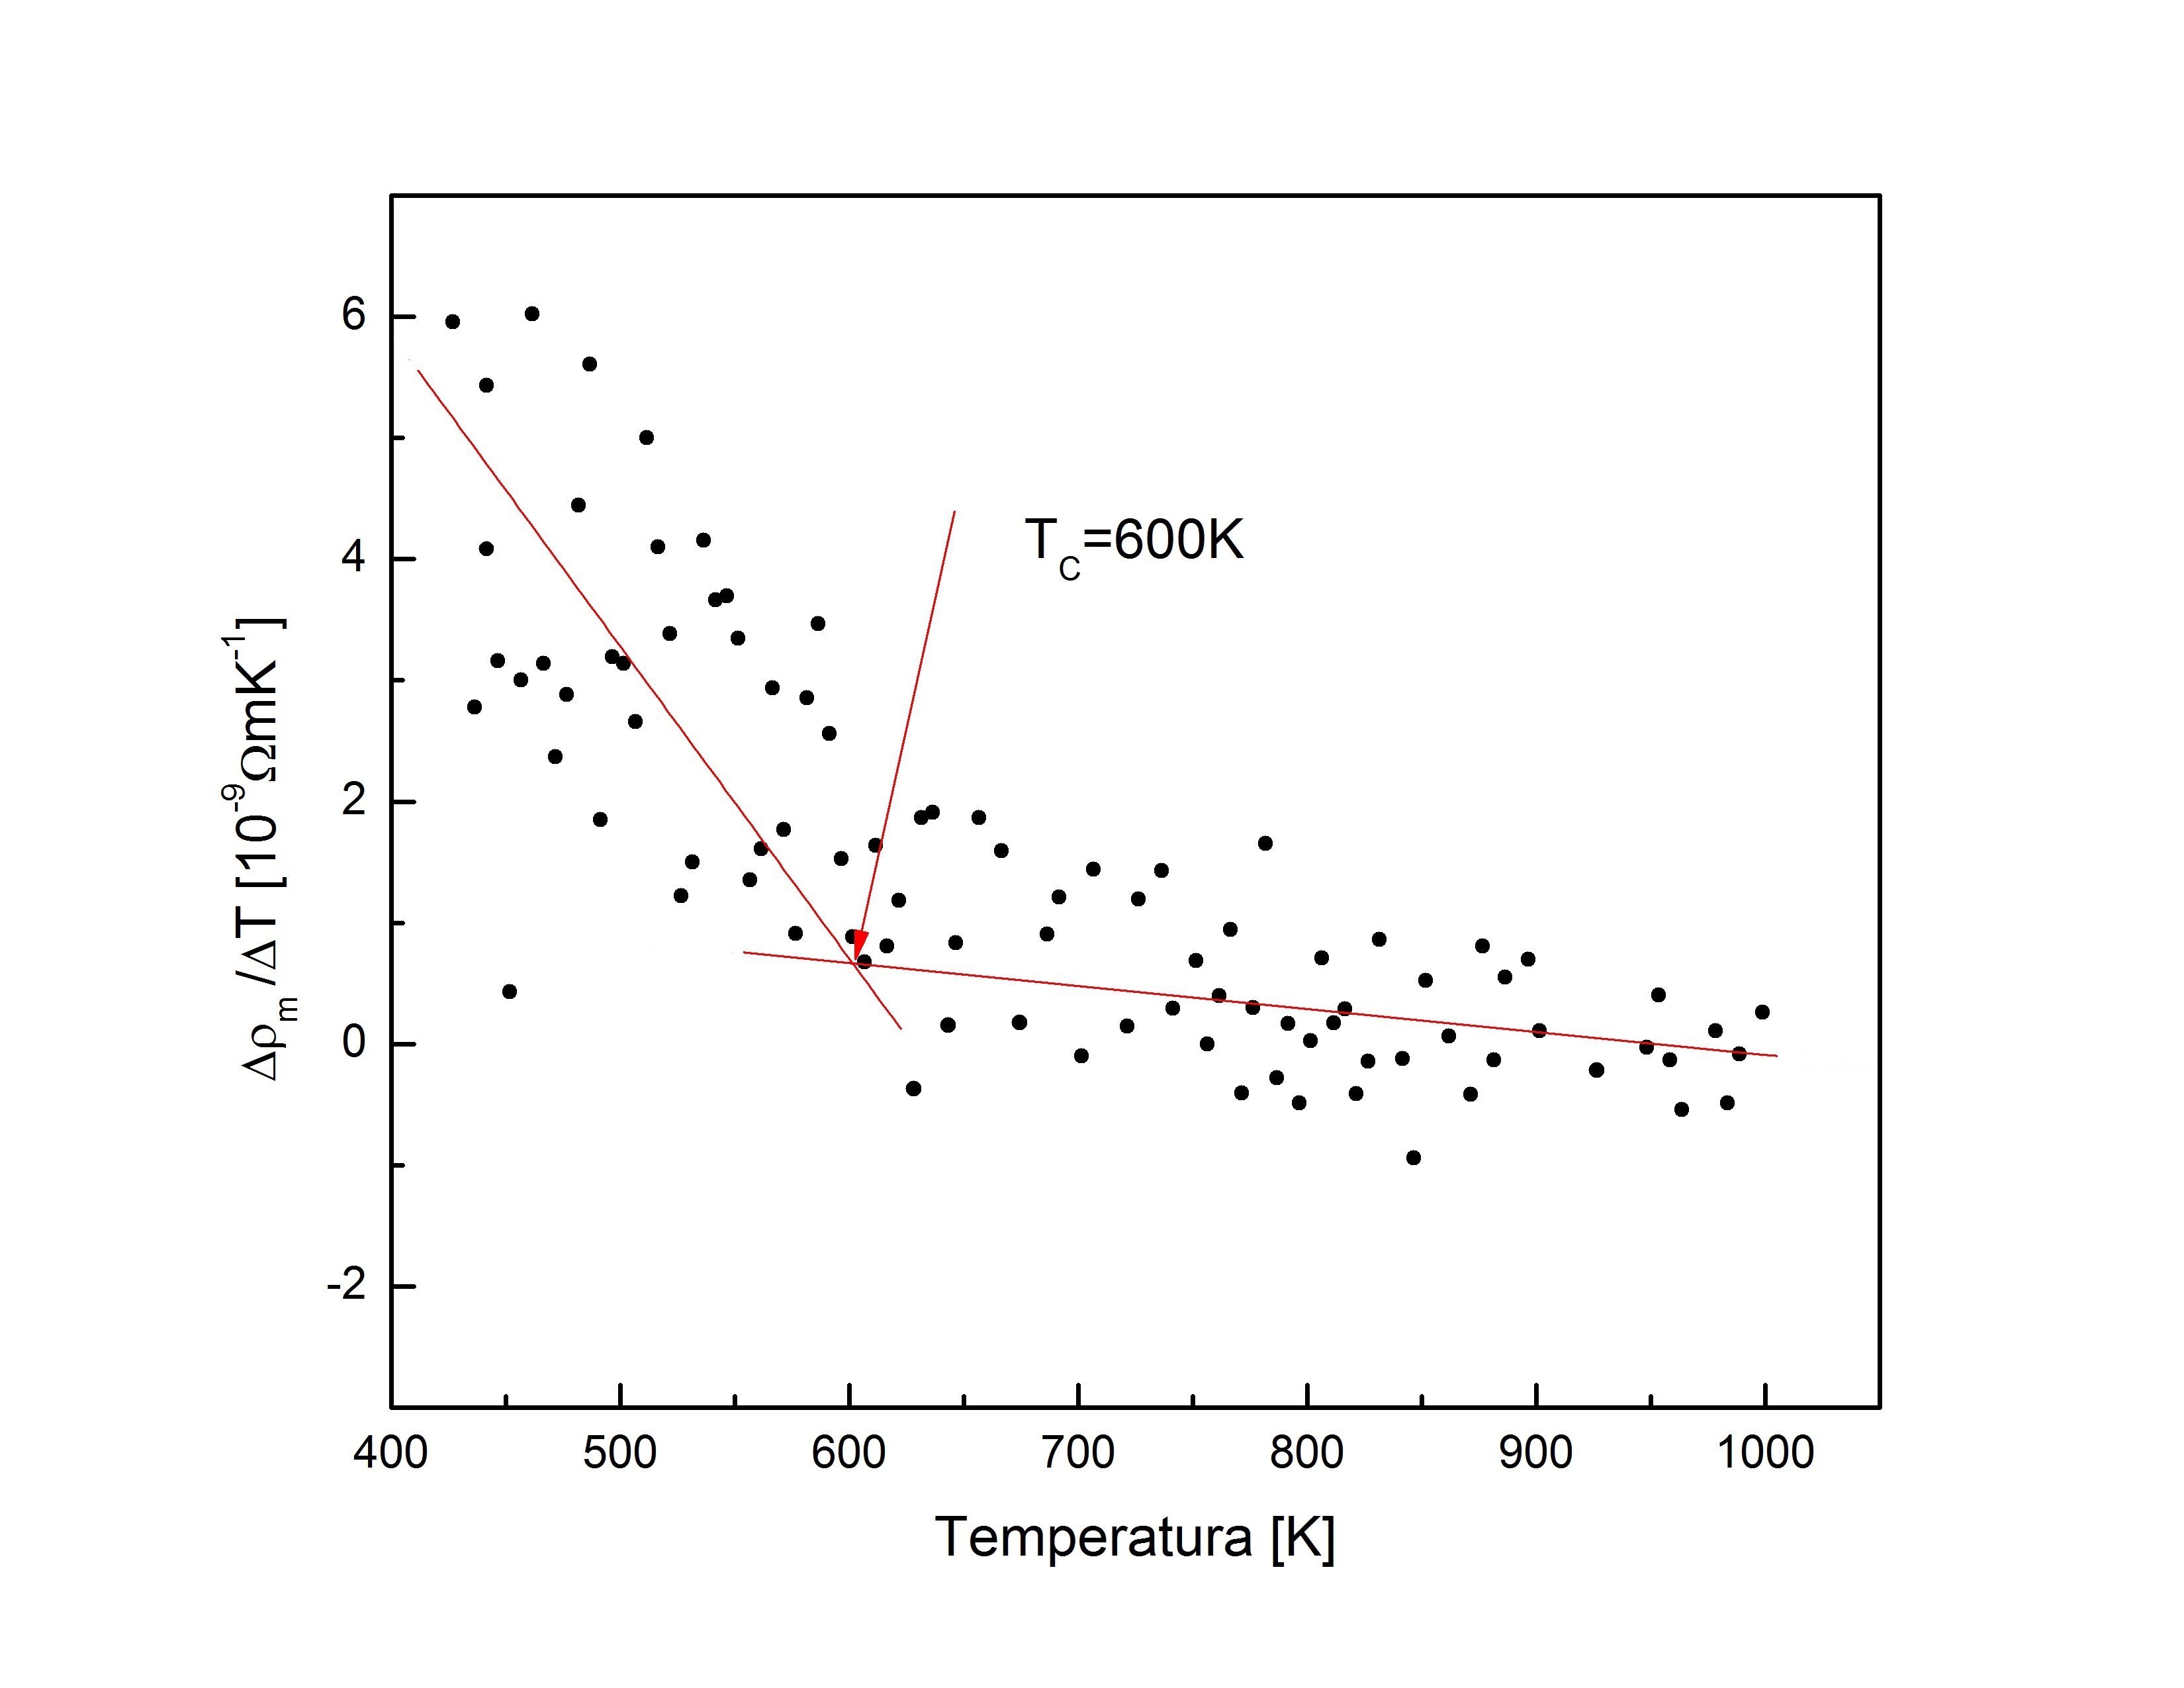
\includegraphics[width =0.8\textwidth]{../img/opor/pochodnaHo}
    \caption{Zależność $\frac{\Delta\rho_m(T)}{\Delta T}$ wraz z wyznaczoną temperaturą Curie $T_C$ dla $HoFe_2$}
    \label{skladoweHo}
\end{figure}


%-----------------------------------------Tb-------------------------------------------------


\begin{figure}[ht]
    \centering
    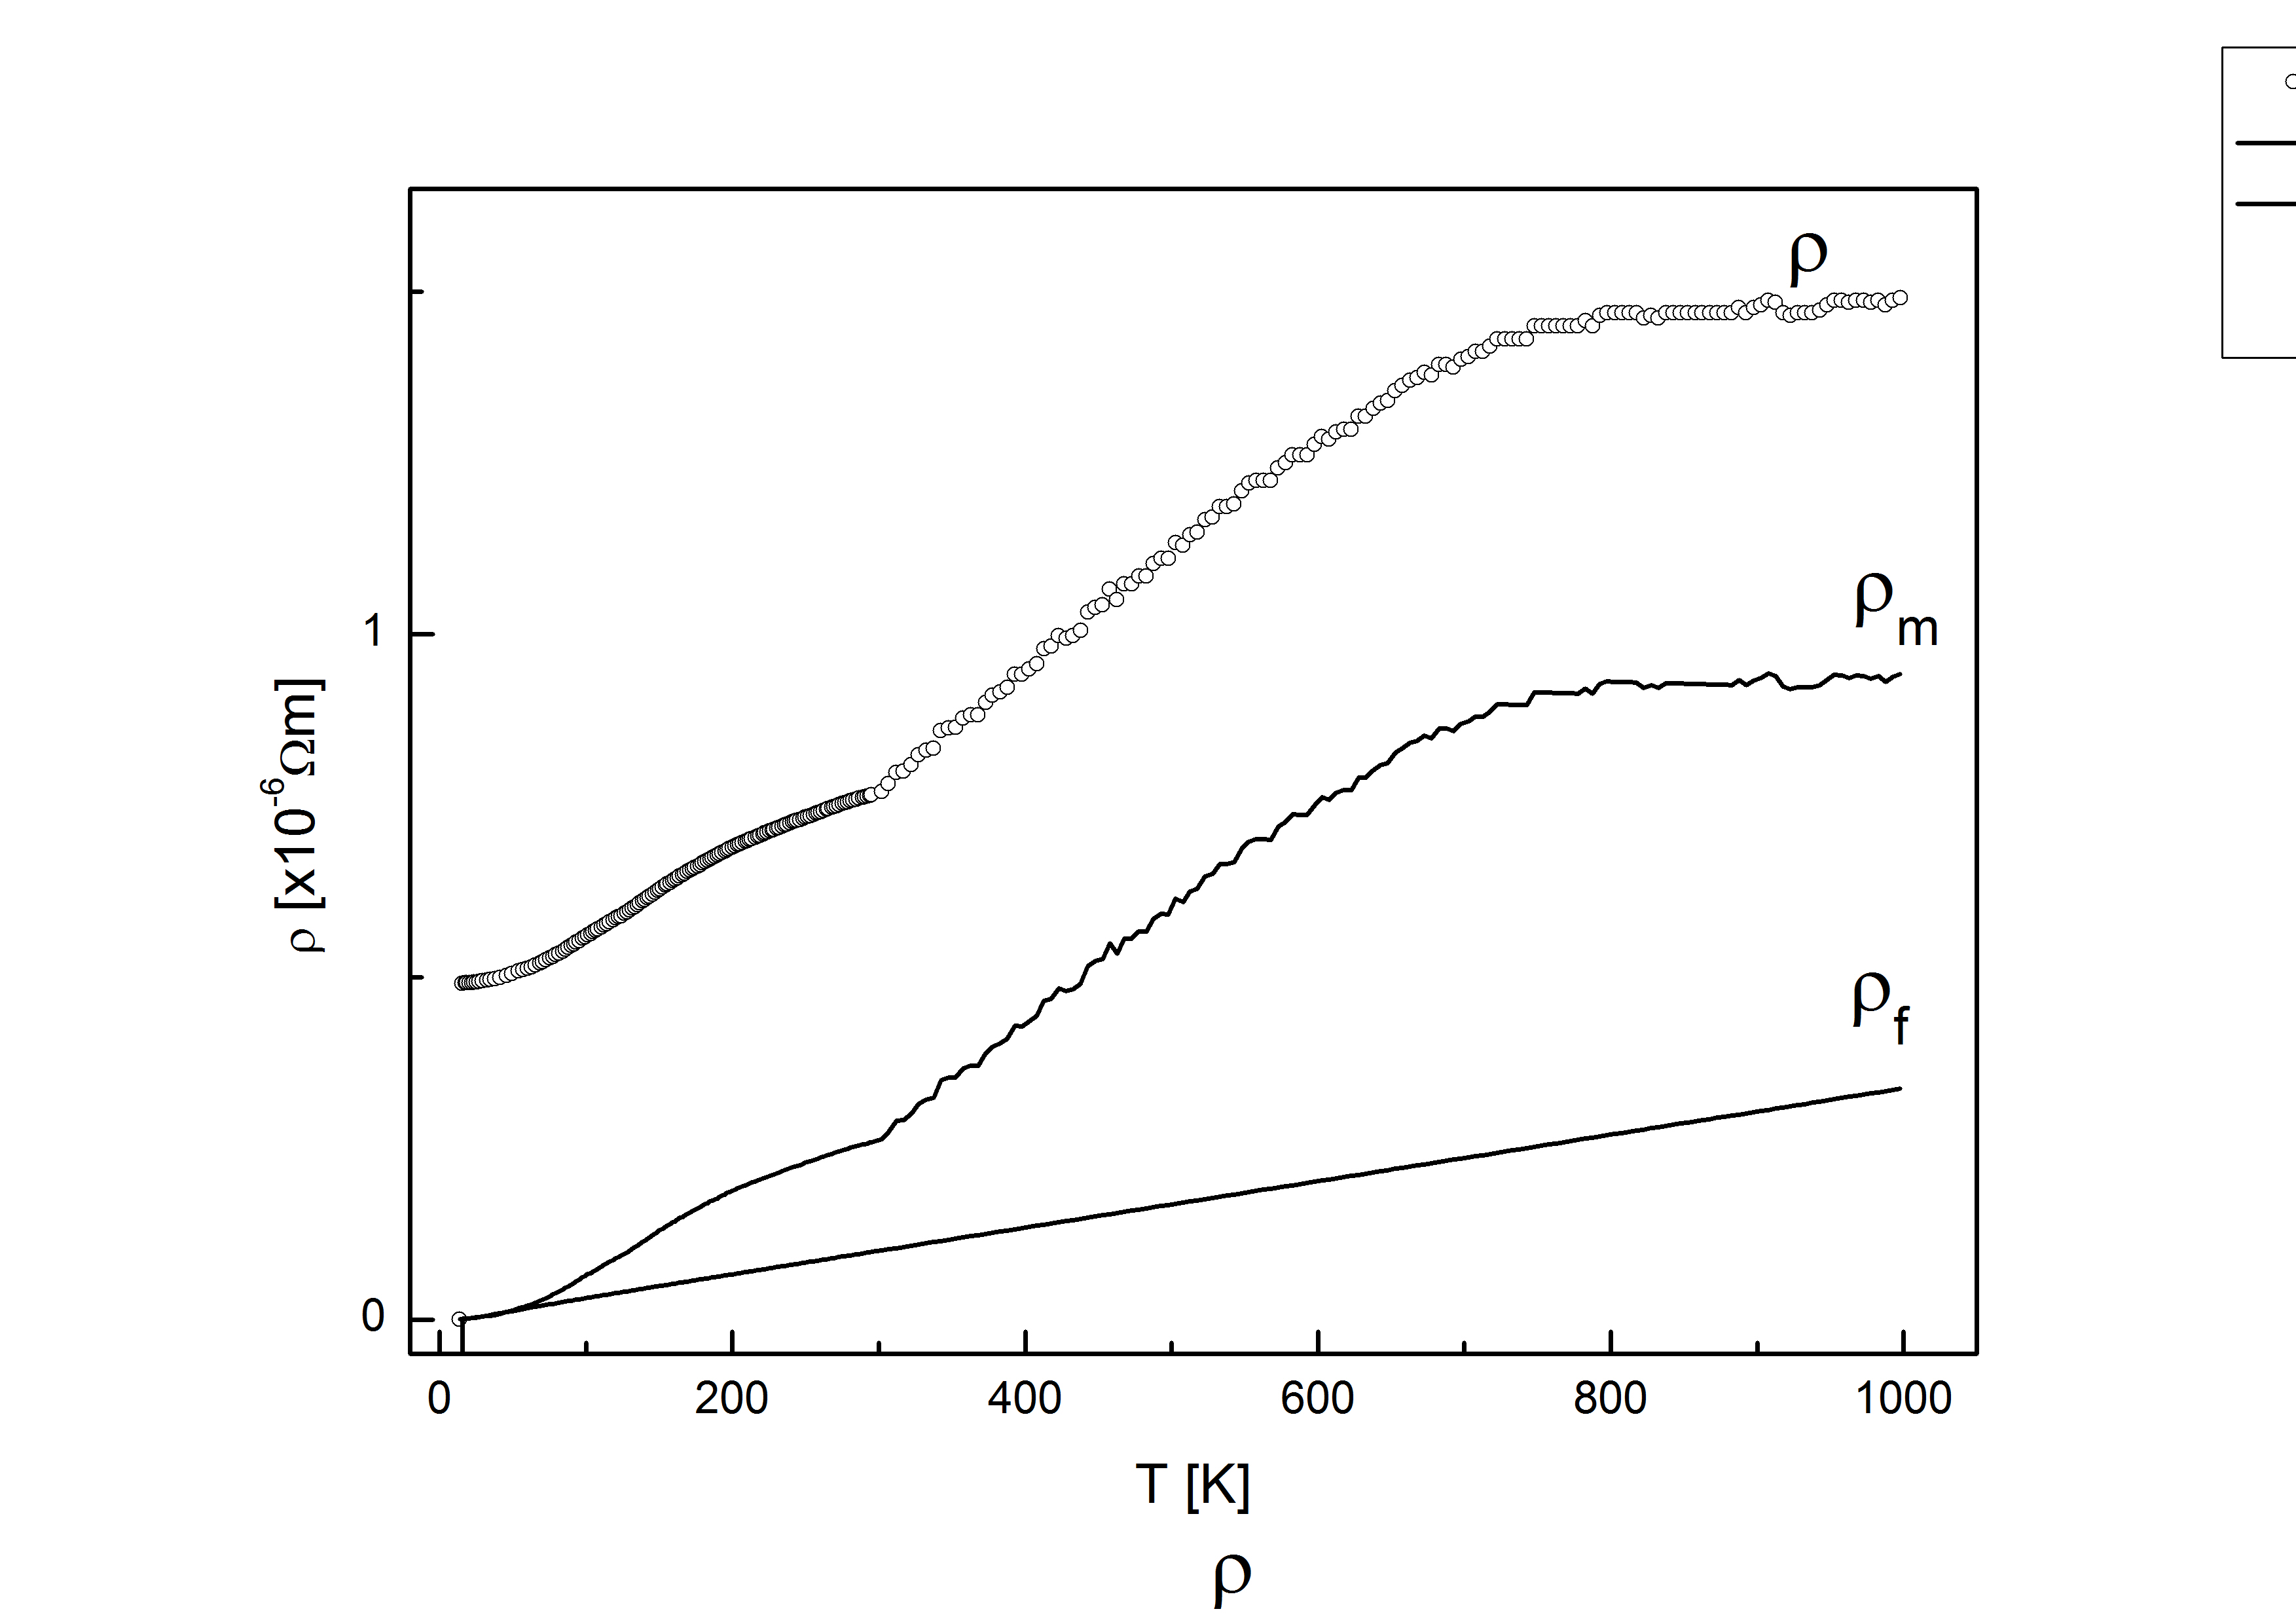
\includegraphics[width =0.8\textwidth]{../img/opor/skladoweTb}
    \caption{Zależność oporności właściwej $\rho$, oporności $\rho_f$ i $\rho_m$ dla $TbFe_2$}
    \label{skladoweTb}
\end{figure}

\begin{figure}[ht]
    \centering
    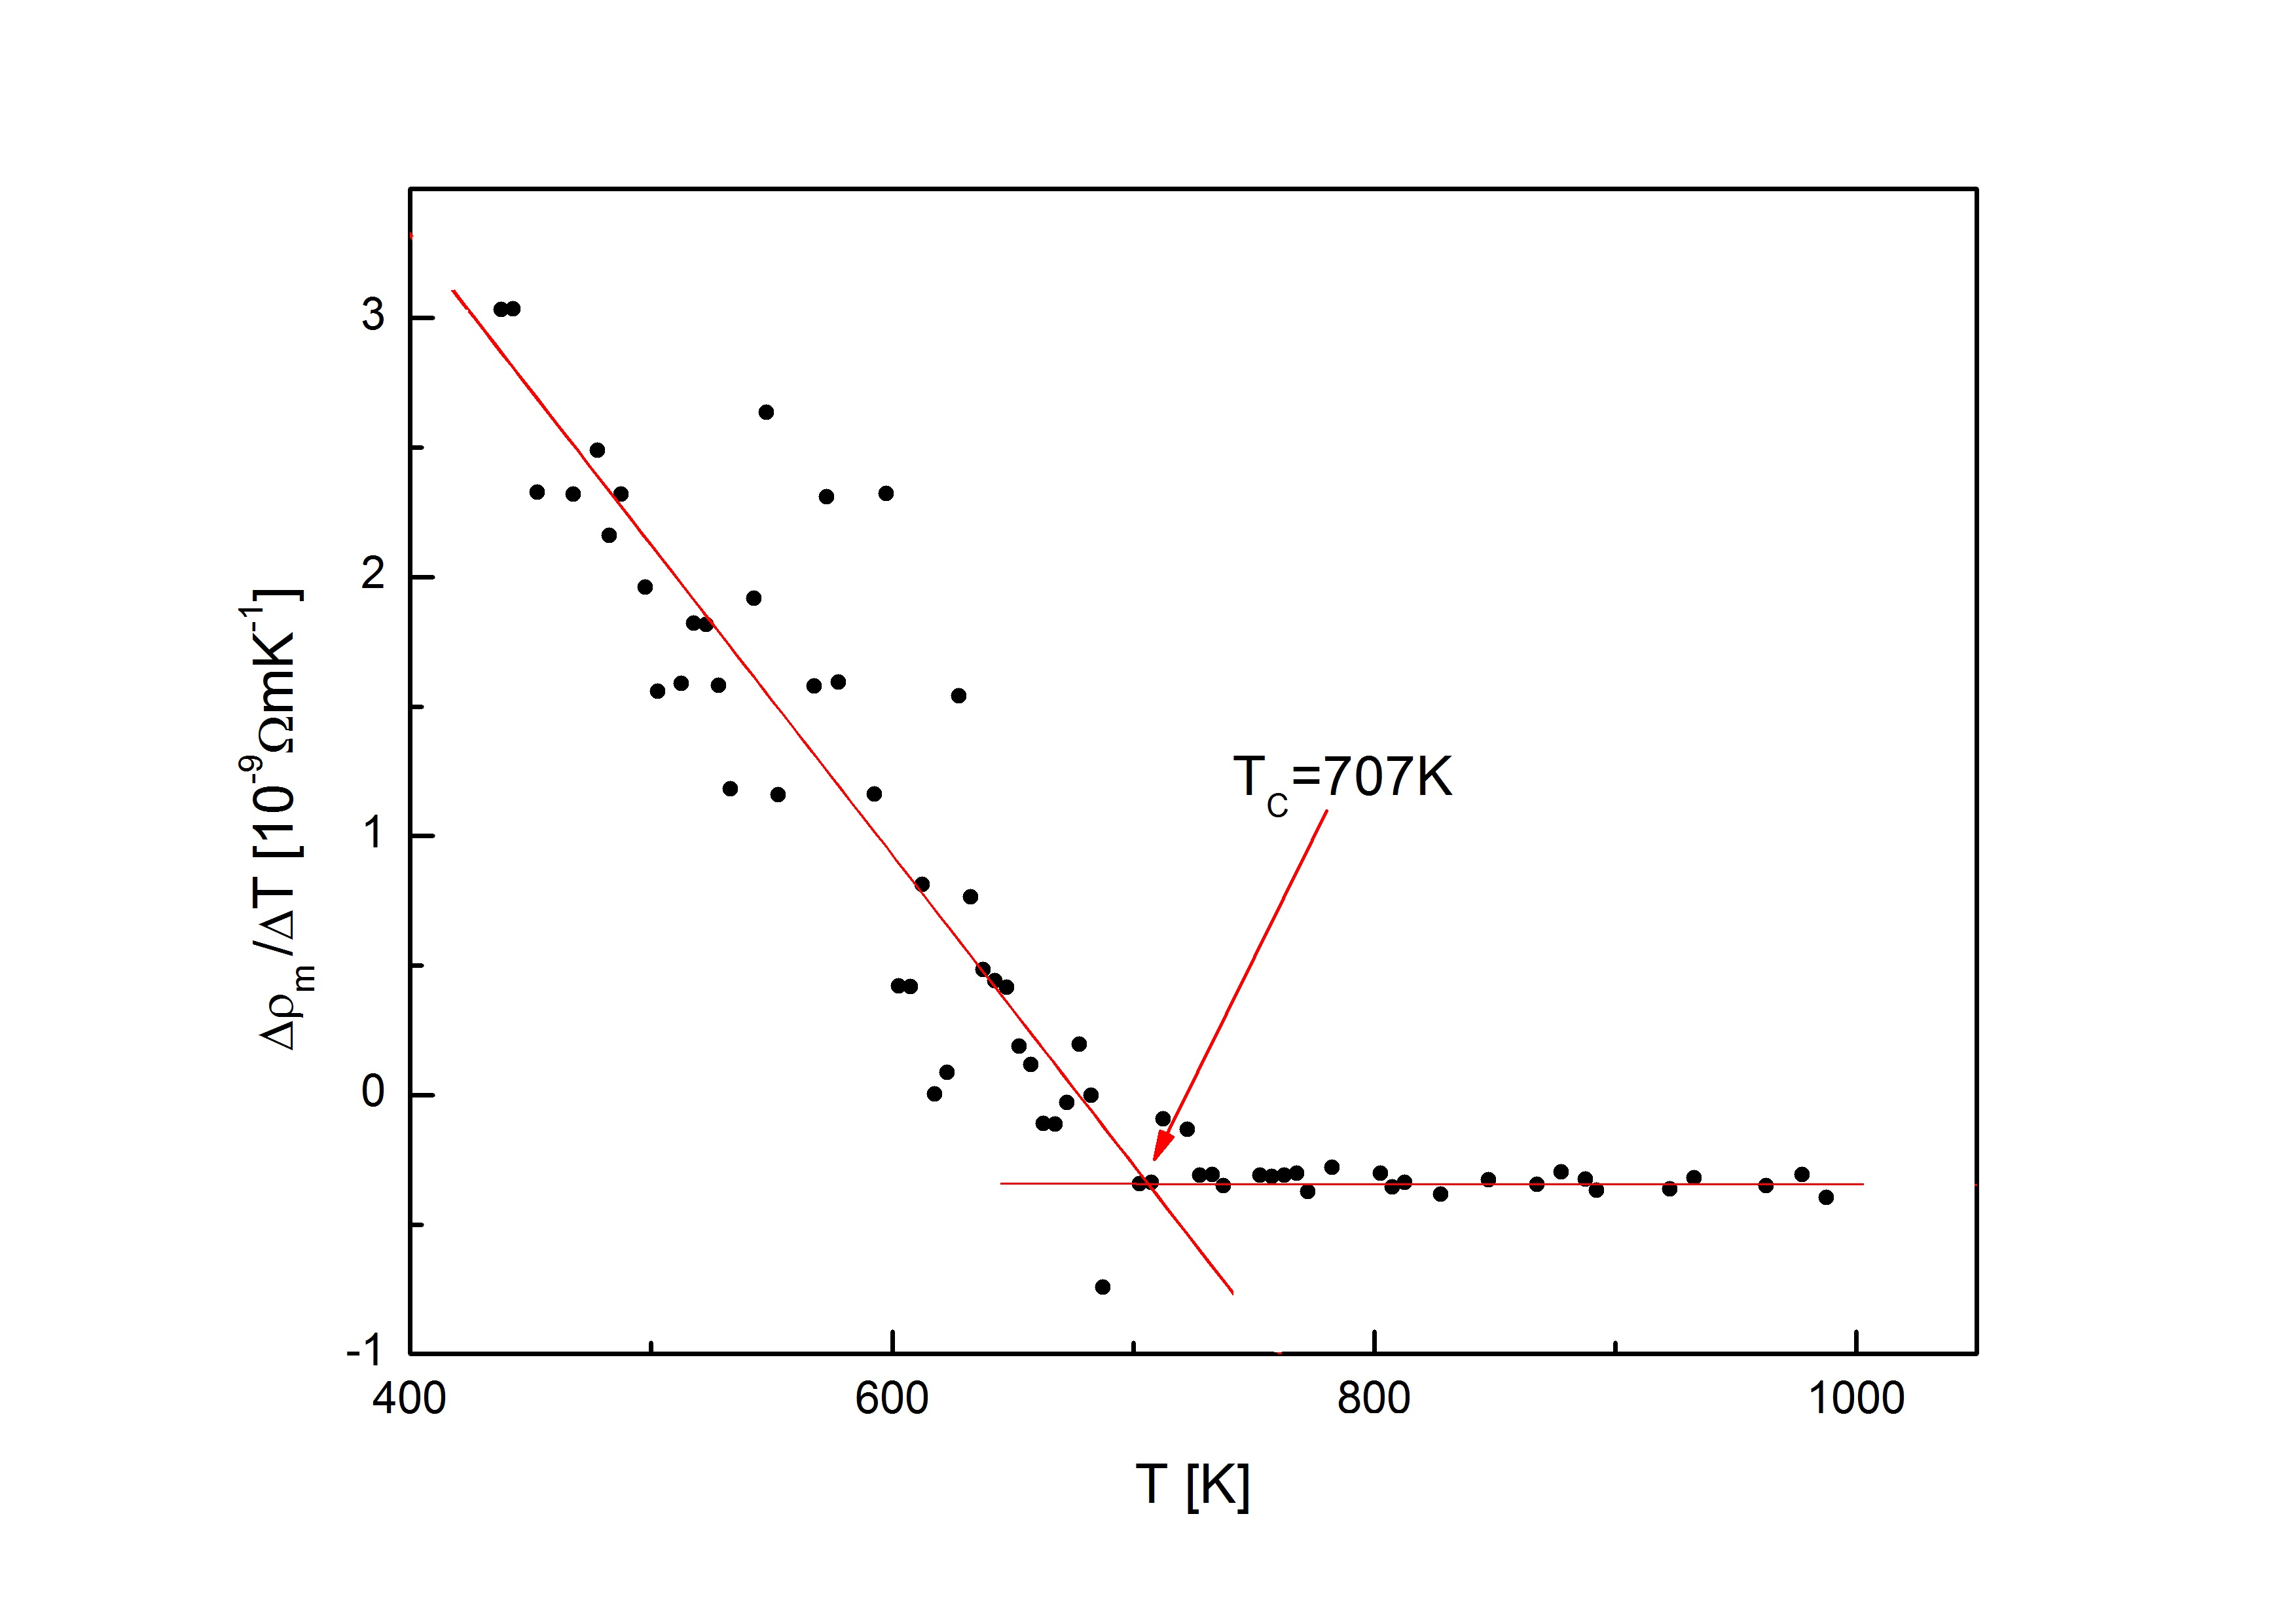
\includegraphics[width =0.8\textwidth]{../img/opor/pochodnaTb}
    \caption{Zależność $\frac{\Delta\rho_m(T)}{\Delta T}$ wraz z wyznaczoną temperaturą Curie $T_C$ dla $TbFe_2$}
    \label{skladoweTb}
\end{figure}


%-----------------------------------------Y-------------------------------------------------


\begin{figure}[ht]
    \centering
    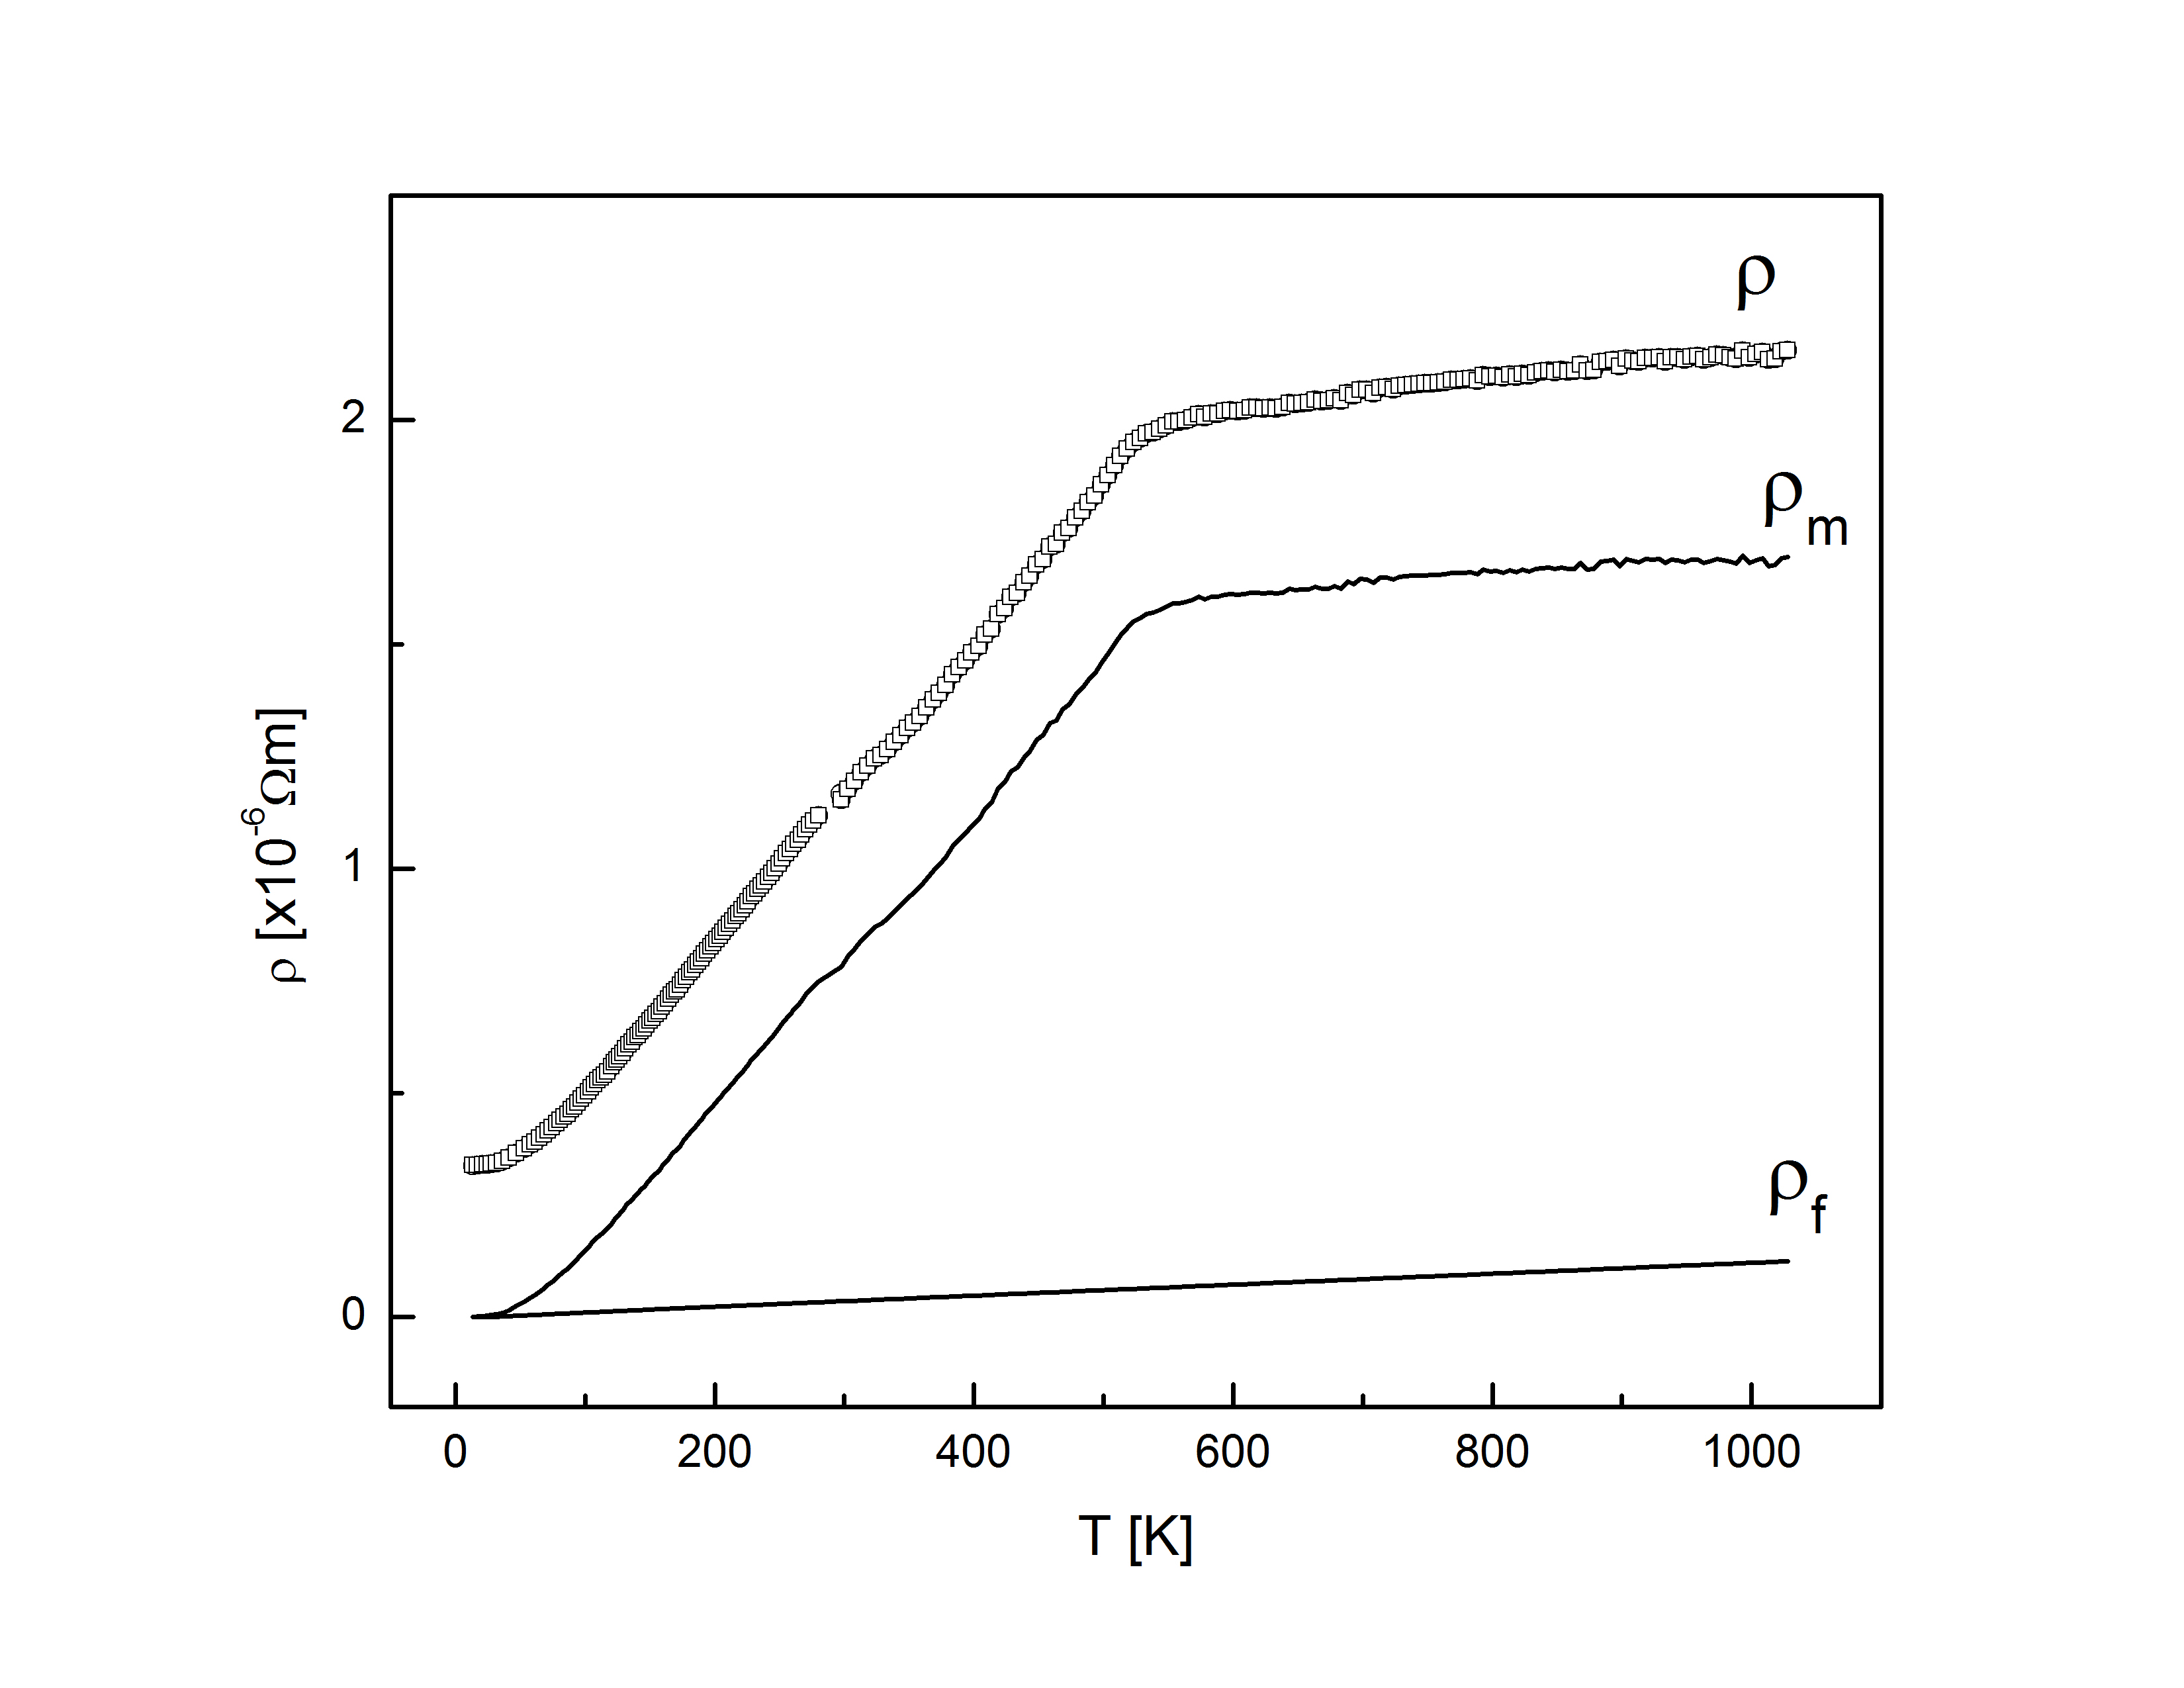
\includegraphics[width =0.8\textwidth]{../img/opor/skladoweY}
    \caption{Zależność oporności właściwej $\rho$, oporności $\rho_f$ i $\rho_m$ dla $YFe_2$}
    \label{skladoweY}
\end{figure}

\begin{figure}[ht]
    \centering
    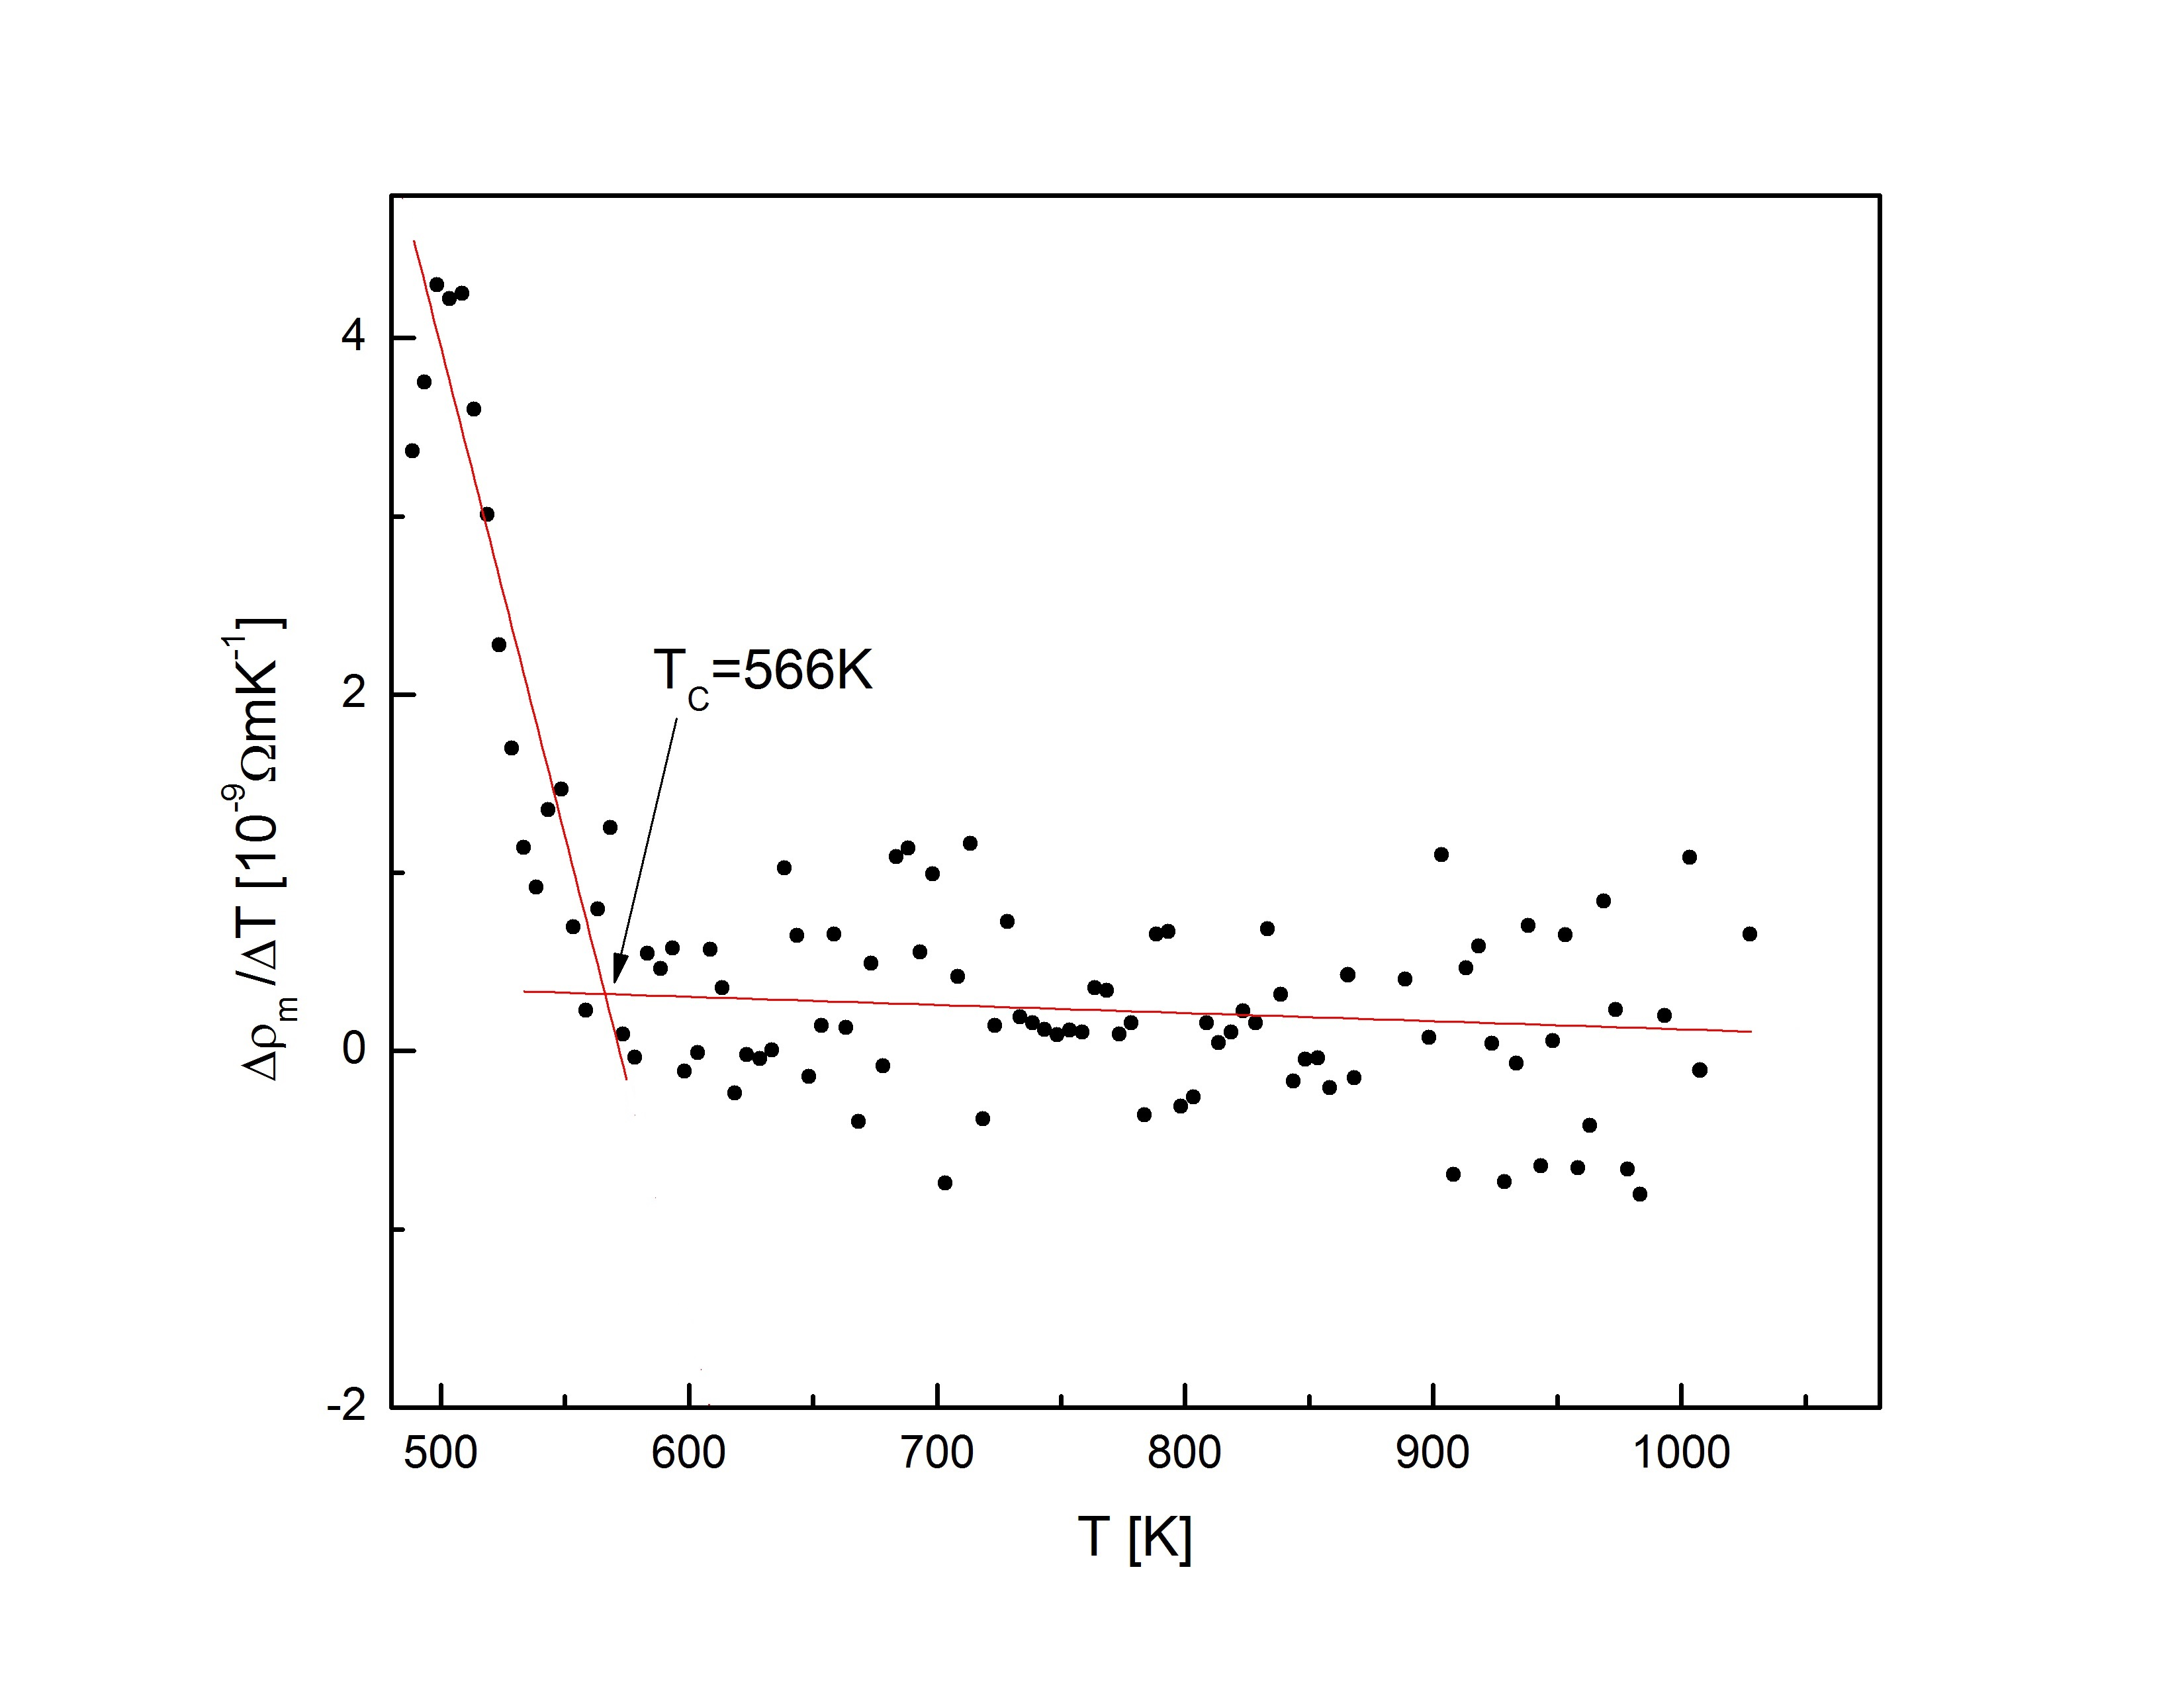
\includegraphics[width =0.8\textwidth]{../img/opor/pochodnaY}
    \caption{Zależność $\frac{\Delta\rho_m(T)}{\Delta T}$ wraz z wyznaczoną temperaturą Curie $T_C$ dla $YFe_2$}
    \label{skladoweY}
\end{figure}


%-----------------------------------------------------------------
%-------------------Parametry oporności---------------------
%-----------------------------------------------------------------
\clearpage
\subsection{Parametry oporności właściwej badanych próbek}

Zebrane dane pomiarowe posłużyły do wyznaczenia wielkości o których była mowa w części teoretycznej. Wartości te zostały zebrane w tabeli \ref{tabParametryOpor}

  \begin{table}[ht]
  \centering
  \footnotesize
  \caption{Wartości wyznaczone na podstawie pomiarów oporności elektrycznej}
  \label{tabParametryOpor}
  \begin{tabular}{|c|c|c|c|c|c|c|c|c|}
    \hline
Związek	&	$\rho_0$	&	$\theta_D$	&	$\rho_{m\infty}$	&	$A_2 $	&	$A_1$	&	$A_3$	&	$R_t $	&	$T_C$ \\
	&	$[10^{-6}{\Omega}m]$	&	$[K]$	&	$ [10^{-6}{\Omega}m]$	&	$ [10^{-6}{\Omega}m/K^2]$	&	$[10^{-6}{\Omega}m/K]$	&	$ [10^{-6}{\Omega}m]$	&	$ [10^{-6}{\Omega}m]$	&	$[K]$		\\\hline
$YFe_2$	&	0,33618	&	168	&	1,694210	&	4,17E+00	&	3,40E+00	&	1,21E-04	&	2,04E-02	&	566	\\\hline
$GdFe_2$	&	0,30418	&	105	&	0,959710	&	4,53E-06	&	8,01E-05	&	1,05E-04	&	1,12E-02	&	766	\\\hline
$TbFe_2$	&	0,48907	&	129	&	0,941520	&	7,81E-08	&	9,91E-09	&	6,06E-05	&	7,86E-03	&	707	\\\hline
$DyFe_2$	&	0,62482	&	42	&	1,166223	&	3,28E-04	&	7,30E-03	&	6,54E-05	&	2,78E-03	&	621	\\\hline
$HoFe_2$	&	0,07195	&	588	&	0,241430	&	1,03E+00	&	2,01E+00	&	2,46E-04	&	1,45E-01	&	600	\\\hline
  \end{tabular}
\end{table}

Otrzymane wartości temperatury Curie badanych związków porównano z wartościami literaturowymi. Wyniki zamieszczono w tabeli \ref{tabTCurie} oraz na wykresie \ref{RysTempCurie}. Kolorem czerwonym zaznaczono punkty pomiarowe, na niebiesko i zielono oznaczono
dane zaczerpnięte kolejno 
z REF DO BIBLIOGRAFIIII. 

  \begin{table}[ht]
  \centering
  \footnotesize
  \caption{Temperatury Curie badanych próbek i wartości literaturowe}
  \label{tabTCurie}
  \begin{tabular}{|c|c|c|c|}
    \hline
Związek	&	Wartości zmierzone [K]	&	Dane literaturowe 1 [K]	&	Dane literaturowe 2 [K]	\\\hline
$YFe_2$	&	566	&	550	&	560	\\\hline
$GdFe_2$	&	766	&	785	&	760	\\\hline
$TbFe_2$	&	707	&	711	&	700	\\\hline
$DyFe_2$	&	621	&	635	&	630	\\\hline
$HoFe_2$	&	600	&	612	&	600	\\\hline  
  \end{tabular}
\end{table}

\begin{figure}[ht]
    \centering
    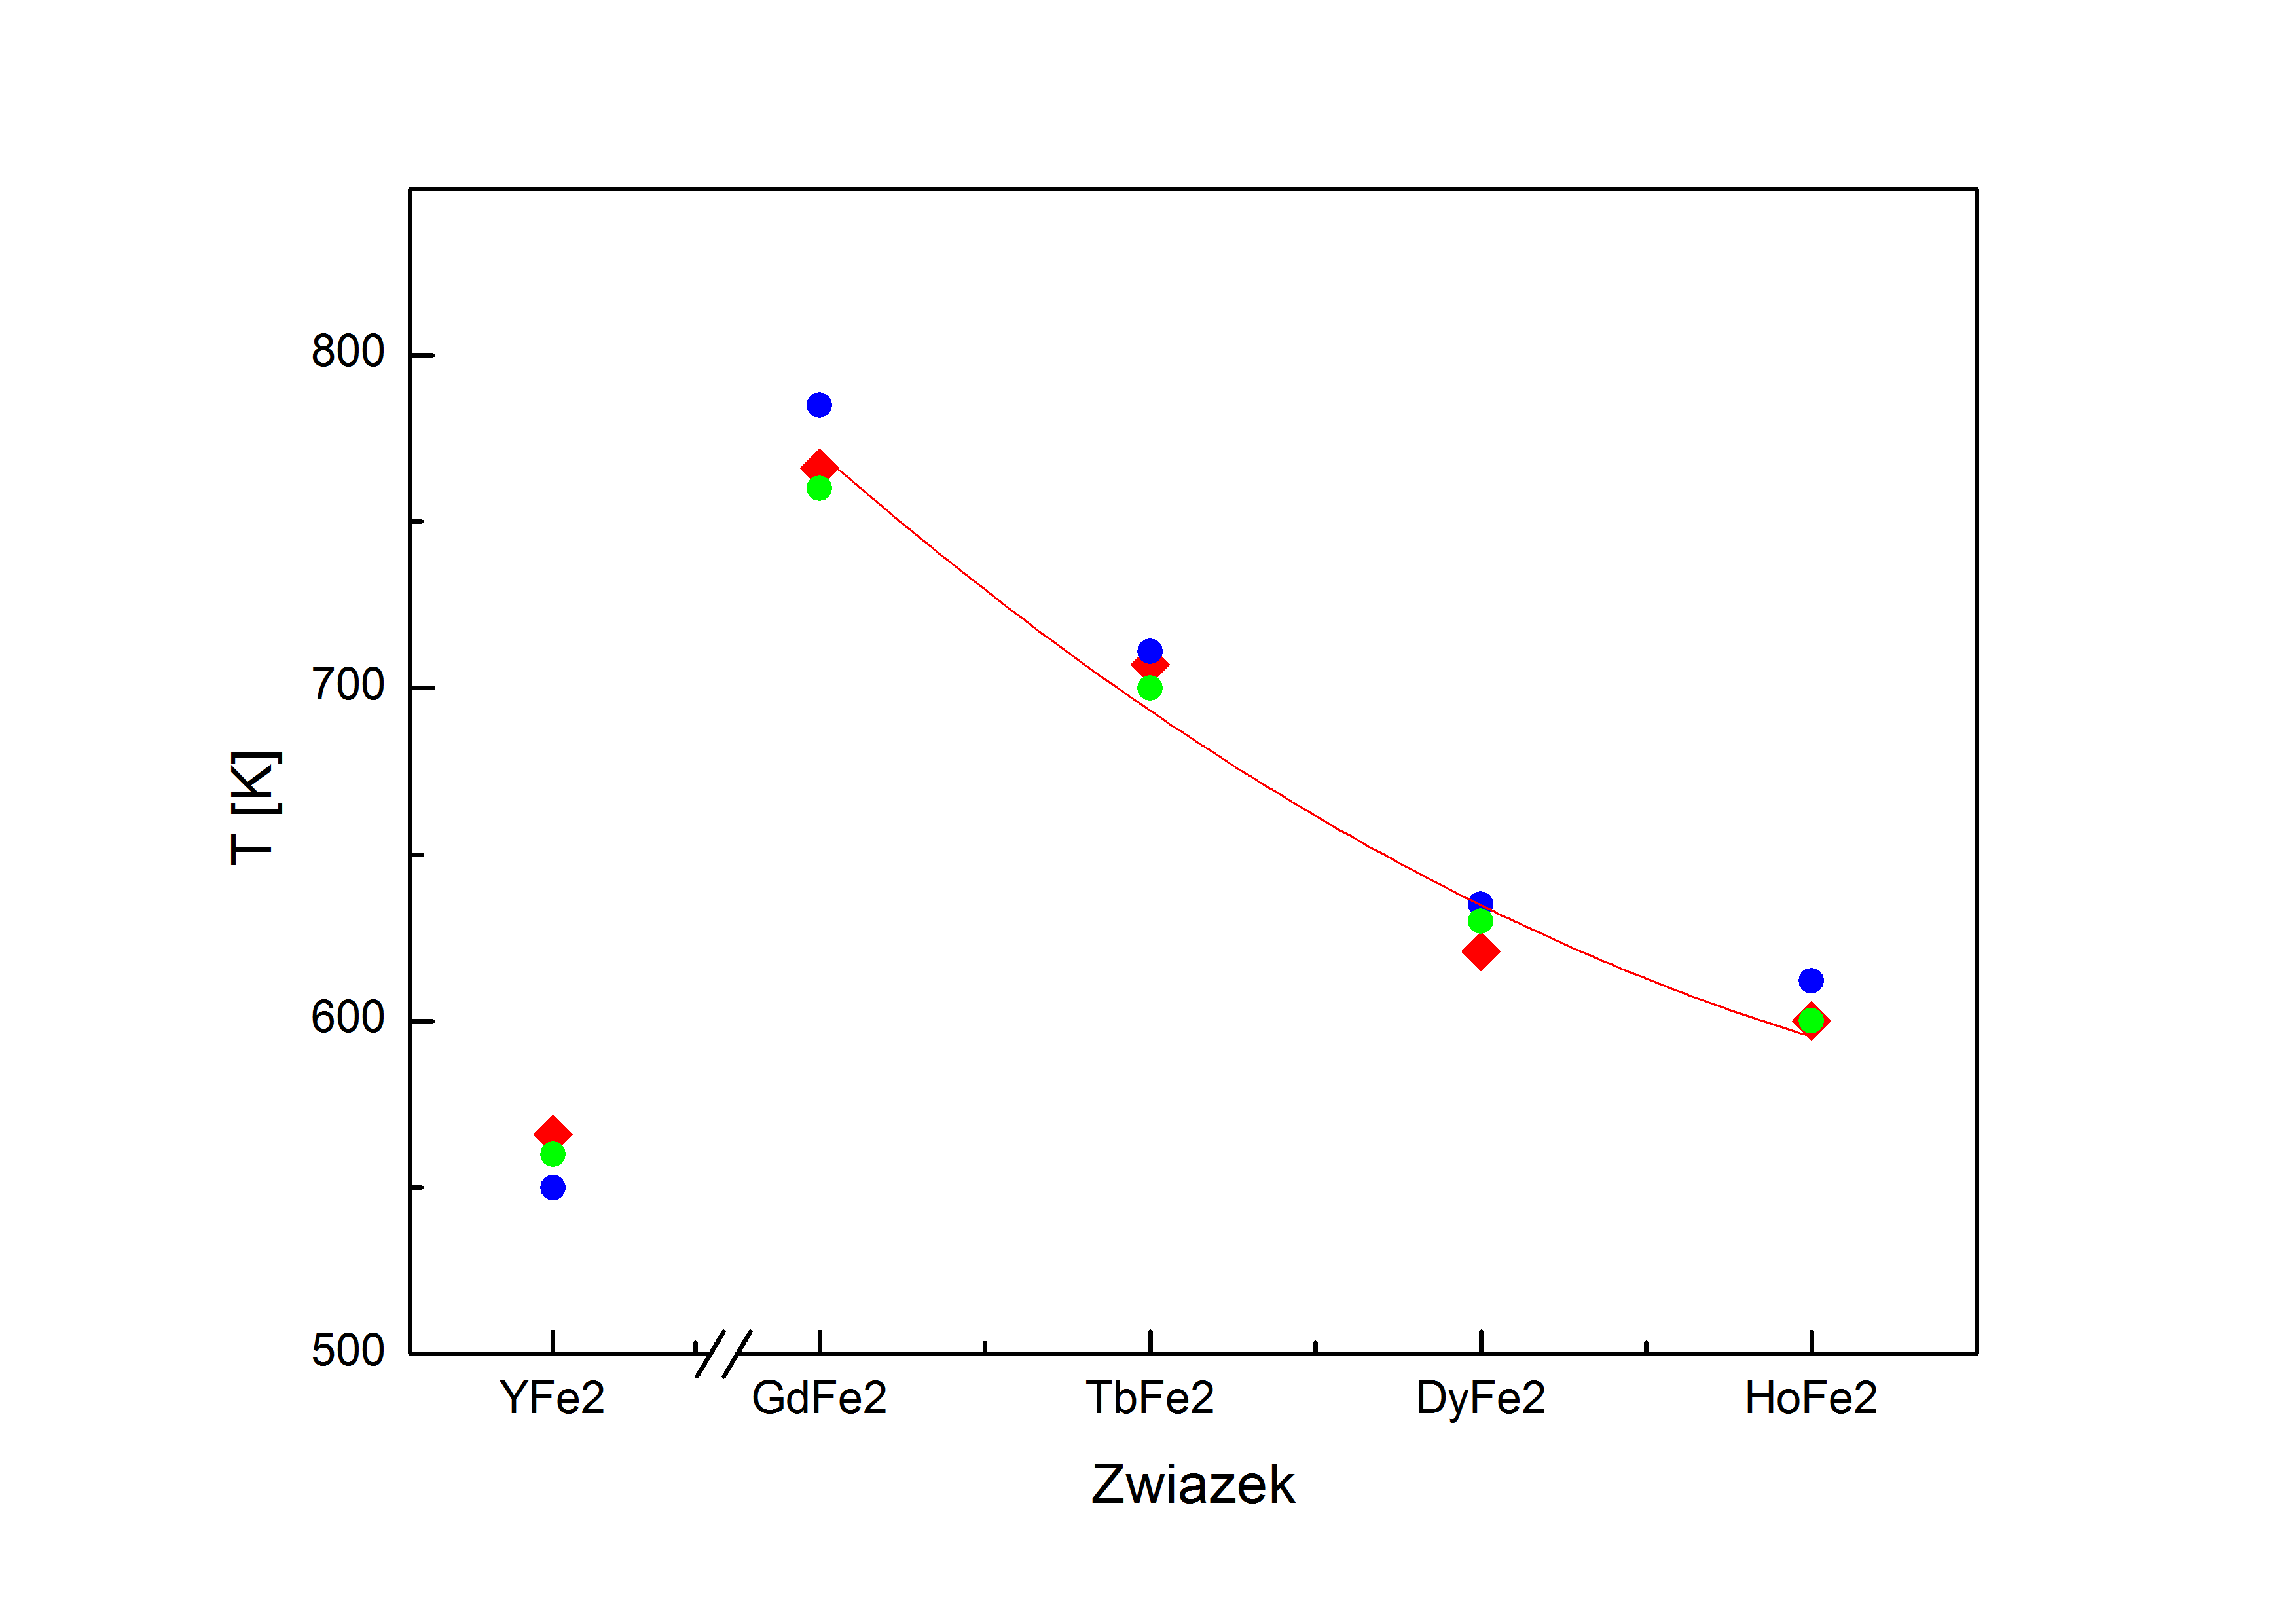
\includegraphics[width =1.0\textwidth]{../img/TempCurie1}
    \caption{Temperatura Curie badanych związków}
    \label{RysTempCurie}
\end{figure}

Do danych z wykresu dopasowano krzywą o równaniu ogólnym 

  \begin{equation}
   y=a_2x^2+a_1x+a_0
    \label{parabola}
  \end{equation}

Wyliczone za pomocą progamu OriginPro równanie ma postać

  \begin{equation}
   T_C=9,5x^2-124,9x+982,4 [K]
    \label{gotowaParabola}
  \end{equation}







\end{document}

\section{Podsumoanie}
\documentclass[a4paper,12pt]{article}

\usepackage[utf8]{inputenc}
\usepackage[T1]{polski}
\usepackage{helvet}
\usepackage{color}
\usepackage{tabularx}
\usepackage[pdftex]{graphicx}
\usepackage{graphicx}
\usepackage{amsmath}
\usepackage{geometry}
\usepackage{multirow}
\usepackage{indentfirst}
\usepackage{wrapfig}
\usepackage{caption}
\usepackage[titletoc]{appendix}
\usepackage[nottoc]{tocbibind}
\usepackage{pdfpages}
\usepackage{hyperref}
\usepackage{chngcntr}
\usepackage{caption}
\usepackage{rotating}
\usepackage{longtable}



\hypersetup{colorlinks,linkcolor=black,citecolor=blue}
\captionsetup{margin=10pt, font={small,it}, labelfont=bf}
\renewcommand{\figurename}{Rys.}
\renewcommand{\appendixname}{Dodatek}



\numberwithin{equation}{section}
\counterwithin{table}{section}
\counterwithin{figure}{section}

\renewcommand{\thefigure}{\thesection.\arabic{figure}}


\linespread{1.3}
\widowpenalty=500 %usuwanie wdów
\clubpenalty=500 %usuwanie bękartów i sierot
\newcommand{\nit}[1]{\textnormal{#1}}

%\geometry{hmargin={2cm, 2cm}, height=10.0in}

\begin{document}
\begin{appendices}
\renewcommand{\thetable}{\Alph{section}.\arabic{table}}

%-----------------------------------------------------------------------------------------
%-------------------------Tablice Technologiczne-------------------------------------
%-----------------------------------------------------------------------------------------

\section{Tablice technologiczne}

%-----------------------------------------Dy-------------------------------------------------

\begin{table}[!ht]
%\centering
\footnotesize
\caption{Tabela technologiczna otrzymania związku $DyFe_{2}$ }
\label{Dytechno}
\begin{tabular}{|c|c|c|c|c|}
\hline
\multicolumn{5}{|c|}{$DyFe_{2} $}\\\hline\hline
	& m wyliczona		&	nadwyżka	& m + nadwyżka	&	m zważona \\\hline
Dy	&	2,8515	&	0,0000	&	2,8515	&	2,8597	\\\hline
Fe	&	4,1485	&	0,1245	&	4,2730	&	4,2855	\\\hline
SUMA	&	7,0000	&	0,1245	&	7,1245	&	7,1452	\\\hline
\multicolumn{5}{|c|}{}\\\cline{1-3}
\multirow{2}{*}{Wielkoć nadważek:}	
	&	Dy 	&	3\%	& 	\multicolumn{2}{c|}{}\\\cline{2-3}	
	&	Fe	&	0\%	&	\multicolumn{2}{c|}{}\\\cline{1-3}
\multicolumn{1}{|c}{topiona:}	&	\multicolumn{1}{c|}{2} 	&	\multicolumn{3}{c|}{}\\\cline{1-4}
\multicolumn{1}{|c}{prąd topienia:}	&	\multicolumn{3}{c|}{10-30-50-75-100-120-140-120-100-75-50-30-10}	&	\\\cline{1-5}
\multicolumn{1}{|c}{płukanie:}	&	\multicolumn{1}{c|}{3}	&	&	\multicolumn{1}{c}{m po top.:}	&	\multicolumn{1}{c|}{7,1415} 	 	\\\cline{1-2}\cline{4-5}
\multicolumn{1}{|c}{próżnia:}	&	\multicolumn{1}{c|}{$5\times10^{-2}mBa$}	&	&	\multicolumn{1}{c}{ubytek:}	&	\multicolumn{1}{c|}{0,0037} 	 	\\\cline{1-2}\cline{4-5}
\multicolumn{1}{|c}{wygrzewana:}	&	\multicolumn{1}{c|}{1h w 1073K }	&	&	\multicolumn{1}{c}{ubytek nadw.:}	&	\multicolumn{1}{c|}{$3\%$} 	 	\\\hline
\end{tabular}
\end{table}

%-----------------------------------------Gd-------------------------------------------------
\begin{table}[!ht]
%\centering
\footnotesize
\caption{Tabela technologiczna otrzymania związku $DdFe_{2}$ }
\label{Gdtechno}
\begin{tabular}{|c|c|c|c|c|}
\hline
 \multicolumn{5}{|c|}{$GdFe_{2} $}\\\hline\hline
	& m wyliczona		&	nadwyżka	& m + nadwyżka	&	m zważona \\\hline
Gd	&	2,9071	&	0,0000	&	2,9071	&	2,9277	\\\hline
Fe	&	4,0929	&	0,1228	&	4,2156	&	4,2454	\\\hline
SUMA	&	7,0000	&	0,1228	&	7,1228	&	7,1731	\\\hline
\multicolumn{5}{|c|}{}\\\cline{1-3}
\multirow{2}{*}{Wielkoć nadważek:}	
	&	Gd 	&	3\%	& 	\multicolumn{2}{c|}{}\\\cline{2-3}	
	&	Fe	&	0\%	&	\multicolumn{2}{c|}{}\\\cline{1-3}
\multicolumn{1}{|c}{topiona:}	&	\multicolumn{1}{c|}{2} 	&	\multicolumn{3}{c|}{}\\\cline{1-4}
\multicolumn{1}{|c}{prąd topienia:}	&	\multicolumn{3}{c|}{10-30-50-75-100-120-140-120-100-75-50-30-10}	&	\\\cline{1-5}
\multicolumn{1}{|c}{płukanie:}	&	\multicolumn{1}{c|}{3}	&	&	\multicolumn{1}{c}{m po top.:}	&	\multicolumn{1}{c|}{7,0896} 	 	\\\cline{1-2}\cline{4-5}
\multicolumn{1}{|c}{próżnia:}	&	\multicolumn{1}{c|}{$5\times10^{-2}mBa$}	&	&	\multicolumn{1}{c}{ubytek:}	&	\multicolumn{1}{c|}{0,0836} 	 	\\\cline{1-2}\cline{4-5}
\multicolumn{1}{|c}{wygrzewana:}	&	\multicolumn{1}{c|}{1h w 1073K }	&	&	\multicolumn{1}{c}{ubytek nadw.:}	&	\multicolumn{1}{c|}{$68\%$} 	 	\\\hline
\end{tabular}
\end{table}

%-----------------------------------------Ho-------------------------------------------------
\begin{table}[!ht]
%\centering
\footnotesize
\caption{Tabela technologiczna otrzymania związku $HoFe_{2}$ }
\label{Hotechno}
\begin{tabular}{|c|c|c|c|c|}
\hline
\multicolumn{5}{|c|}{$HoFe_{2} $}\\\hline\hline
	& m wyliczona		&	nadwyżka	& m + nadwyżka	&	m zważona \\\hline
Ho	&	2,8264	&	0,0000	&	2,8264	&	2,8097	\\\hline
Fe	&	4,1736	&	0,1252	&	4,2988	&	4,2739	\\\hline
SUMA	&	7,0000	&	0,1252	&	7,1252	&	7,0836	\\\hline
\multicolumn{5}{|c|}{}\\\cline{1-3}
\multirow{2}{*}{Wielkoć nadważek:}	
	&	Ho 	&	3\%	& 	\multicolumn{2}{c|}{}\\\cline{2-3}	
	&	Fe	&	0\%	&	\multicolumn{2}{c|}{}\\\cline{1-3}
\multicolumn{1}{|c}{topiona:}	&	\multicolumn{1}{c|}{2} 	&	\multicolumn{3}{c|}{}\\\cline{1-4}
\multicolumn{1}{|c}{prąd topienia:}	&	\multicolumn{3}{c|}{10-30-50-75-100-120-140-120-100-75-50-30-10}	&	\\\cline{1-5}
\multicolumn{1}{|c}{płukanie:}	&	\multicolumn{1}{c|}{3}	&	&	\multicolumn{1}{c}{m po top.:}	&	\multicolumn{1}{c|}{7,0741} 	 	\\\cline{1-2}\cline{4-5}
\multicolumn{1}{|c}{próżnia:}	&	\multicolumn{1}{c|}{$5\times10^{-2}mBa$}	&	&	\multicolumn{1}{c}{ubytek:}	&	\multicolumn{1}{c|}{0,0095} 	 	\\\cline{1-2}\cline{4-5}
\multicolumn{1}{|c}{wygrzewana:}	&	\multicolumn{1}{c|}{1h w 1073K }	&	&	\multicolumn{1}{c}{ubytek nadw.:}	&	\multicolumn{1}{c|}{$8\%$} 	 	\\\hline
\end{tabular}
\end{table}

%-----------------------------------------Tb-------------------------------------------------
\begin{table}[!ht]
%\centering
\footnotesize
\caption{Tabela technologiczna otrzymania związku $TbFe_{2}$ }
\label{Tbtechno}
\begin{tabular}{|c|c|c|c|c|}
\hline
\multicolumn{5}{|c|}{$TbFe_{2} $}\\\hline\hline
	& m wyliczona		&	nadwyżka	& m + nadwyżka	&	m zważona \\\hline
Tb	&	2,8891	&	0,0000	&	2,8891	&	2,9105	\\\hline
Fe	&	4,1109	&	0,1233	&	4,2342	&	4,2659	\\\hline
SUMA	&	7,0000	&	0,1233	&	7,1233	&	7,1764	\\\hline
\multicolumn{5}{|c|}{}\\\cline{1-3}
\multirow{2}{*}{Wielkoć nadważek:}	
	&	Tb 	&	3\%	& 	\multicolumn{2}{c|}{}\\\cline{2-3}	
	&	Fe	&	0\%	&	\multicolumn{2}{c|}{}\\\cline{1-3}
\multicolumn{1}{|c}{topiona:}	&	\multicolumn{1}{c|}{2} 	&	\multicolumn{3}{c|}{}\\\cline{1-4}
\multicolumn{1}{|c}{prąd topienia:}	&	\multicolumn{3}{c|}{10-30-50-75-100-120-140-120-100-75-50-30-10}	&	\\\cline{1-5}
\multicolumn{1}{|c}{płukanie:}	&	\multicolumn{1}{c|}{3}	&	&	\multicolumn{1}{c}{m po top.:}	&	\multicolumn{1}{c|}{7,0519} 	 	\\\cline{1-2}\cline{4-5}
\multicolumn{1}{|c}{próżnia:}	&	\multicolumn{1}{c|}{$5\times10^{-2}mBa$}	&	&	\multicolumn{1}{c}{ubytek:}	&	\multicolumn{1}{c|}{0,1245} 	 	\\\cline{1-2}\cline{4-5}
\multicolumn{1}{|c}{wygrzewana:}	&	\multicolumn{1}{c|}{1h w 1073K }	&	&	\multicolumn{1}{c}{ubytek nadw.:}	&	\multicolumn{1}{c|}{$101\%$} 	 	\\\hline
\end{tabular}
\end{table}

%-----------------------------------------Y-------------------------------------------------
\clearpage
\begin{table}[h]
%\centering
\footnotesize
\caption{Tabela technologiczna otrzymania związku $YFe_{2}$ }
\label{Ytechno}
\begin{tabular}{|c|c|c|c|c|}
\hline
\multicolumn{5}{|c|}{$YFe_{2} $}\\\hline\hline
	& m wyliczona		&	nadwyżka	& m + nadwyżka	&	m zważona \\\hline
Y	&	3,8976	&	0,0000	&	3,8976	&	3,9028	\\\hline
Fe	&	3,1024	&	0,0931	&	3,1955	&	3,2014	\\\hline
SUMA	&	7,0000	&	0,0931	&	7,0931	&	7,1042	\\\hline
\multicolumn{5}{|c|}{}\\\cline{1-3}
\multirow{2}{*}{Wielkoć nadważek:}	
	&	Y 	&	3\%	& 	\multicolumn{2}{c|}{}\\\cline{2-3}	
	&	Fe	&	0\%	&	\multicolumn{2}{c|}{}\\\cline{1-3}
\multicolumn{1}{|c}{topiona:}	&	\multicolumn{1}{c|}{2} 	&	\multicolumn{3}{c|}{}\\\cline{1-4}
\multicolumn{1}{|c}{prąd topienia:}	&	\multicolumn{3}{c|}{10-30-50-75-100-120-140-120-100-75-50-30-10}	&	\\\cline{1-5}
\multicolumn{1}{|c}{płukanie:}	&	\multicolumn{1}{c|}{3}	&	&	\multicolumn{1}{c}{m po top.:}	&	\multicolumn{1}{c|}{6,9851} 	 	\\\cline{1-2}\cline{4-5}
\multicolumn{1}{|c}{próżnia:}	&	\multicolumn{1}{c|}{$5\times10^{-2}mBa$}	&	&	\multicolumn{1}{c}{ubytek:}	&	\multicolumn{1}{c|}{0,1191} 	 	\\\cline{1-2}\cline{4-5}
\multicolumn{1}{|c}{wygrzewana:}	&	\multicolumn{1}{c|}{1h w 1073K }	&	&	\multicolumn{1}{c}{ubytek nadw.:}	&	\multicolumn{1}{c|}{$128\%$} 	 	\\\hline
\end{tabular}
\end{table}


%-----------------------------------------------------------------------------------------
%-------------------------Tabele rentgenograficzne-------------------------------------
%-----------------------------------------------------------------------------------------
\clearpage
 \section{Tabele rentgenograficzne}
 
%-----------------------------------------Dy-------------------------------------------------
%%\centering

  \label{DyRentgenTab}
  \scriptsize
  \begin{longtable}[c]{|c|c|c|c|c|c|c|}
\caption{Dane strukturaln ezwiązku $DyFe_2$}\\
  \hline
  
    $d_{hkl}$ [\AA]&	h	k	l&$2\theta$ $\left[ ^{\circ}\right]$&$\Gamma$ $\left[ ^{\circ}\right]$&$I_{obs}$&$I_{calc}$	&$I_{obs}$ - $I_{calc}$	\\\hline\hline
2,592818	&	2   2   0	&	15,723	&	0,235	&	239,6	&	240,5	&	-0,9	\\\hline
2,211162	&	3   1   1	&	18,459	&	0,235	&	351,3	&	365,0	&	-13,7	\\\hline
2,117027	&	2   2   2	&	19,288	&	0,235	&	66,5	&	49,8	&	16,7	\\\hline
1,833399	&	4   0   0	&	22,307	&	0,235	&	5,2	&	3,9	&	1,3	\\\hline
1,682442	&	3   3   1	&	24,338	&	0,235	&	2,8	&	18,4	&	-15,6	\\\hline
1,496964	&	4   2   2	&	27,409	&	0,235	&	102,1	&	102,1	&	0,0	\\\hline
1,411351	&	3   3   3	&	29,107	&	0,235	&	30,4	&	31,0	&	-0,6	\\\hline
1,411351	&	5   1   1	&	29,107	&	0,235	&	91,1	&	93,0	&	-1,9	\\\hline
1,296409	&	4   4   0	&	31,753	&	0,235	&	104,9	&	89,1	&	15,8	\\\hline
1,239604	&	5   3   1	&	33,249	&	0,235	&	16,5	&	15,7	&	0,8	\\\hline
1,222266	&	4   4   2	&	33,735	&	0,235	&	0,0	&	0,0	&	0,0	\\\hline
1,159543	&	6   2   0	&	35,619	&	0,234	&	51,7	&	43,8	&	7,9	\\\hline
1,118363	&	5   3   3	&	36,977	&	0,234	&	33,5	&	40,8	&	-7,3	\\\hline
1,105581	&	6   2   2	&	37,420	&	0,234	&	14,6	&	15,2	&	-0,6	\\\hline
1,058513	&	4   4   4	&	39,151	&	0,234	&	2,2	&	1,5	&	0,7	\\\hline
1,026909	&	5   5   1	&	40,407	&	0,234	&	2,7	&	4,4	&	-1,7	\\\hline
1,026909	&	7   1   1	&	40,407	&	0,234	&	2,7	&	4,4	&	-1,7	\\\hline
0,979993	&	6   4   2	&	42,433	&	0,234	&	51,5	&	47,7	&	3,8	\\\hline
0,954753	&	5   5   3	&	43,611	&	0,234	&	23,2	&	22,2	&	1,0	\\\hline
0,954753	&	7   3   1	&	43,611	&	0,234	&	46,4	&	44,3	&	2,1	\\\hline
0,916699	&	8   0   0	&	45,521	&	0,234	&	12,6	&	11,9	&	0,7	\\\hline
0,895941	&	7   3   3	&	46,637	&	0,234	&	3,3	&	2,8	&	0,5	\\\hline
0,889329	&	6   4   4	&	47,004	&	0,234	&	0,0	&	0,0	&	0,0	\\\hline
0,864273	&	6   6   0	&	48,453	&	0,234	&	7,3	&	7,3	&	0,0	\\\hline
0,864273	&	8   2   2	&	48,453	&	0,234	&	14,6	&	14,7	&	-0,1	\\\hline
0,846811	&	5   5   5	&	49,519	&	0,234	&	4,3	&	4,5	&	-0,2	\\\hline
0,846811	&	7   5   1	&	49,519	&	0,234	&	25,6	&	27,1	&	-1,5	\\\hline
0,841221	&	6   6   2	&	49,870	&	0,233	&	4,0	&	4,5	&	-0,5	\\\hline
0,819921	&	8   4   0	&	51,258	&	0,233	&	1,8	&	2,1	&	-0,3	\\\hline
0,804967	&	7   5   3	&	52,281	&	0,233	&	3,3	&	3,8	&	-0,5	\\\hline
0,804967	&	9   1   1	&	52,281	&	0,233	&	1,7	&	1,9	&	-0,2	\\\hline
0,800161	&	8   4   2	&	52,619	&	0,233	&	0,0	&	0,0	&	0,0	\\\hline
0,781764	&	6   6   4	&	53,957	&	0,233	&	9,7	&	9,7	&	0,0	\\\hline
0,768770	&	9   3   1	&	54,945	&	0,233	&	17,2	&	17,8	&	-0,6	\\\hline
0,748482	&	8   4   4	&	56,566	&	0,233	&	17,1	&	19,8	&	-2,7	\\\hline
0,737054	&	7   5   5	&	57,524	&	0,233	&	1,5	&	1,3	&	0,2	\\\hline
0,737054	&	7   7   1	&	57,524	&	0,233	&	1,5	&	1,3	&	0,2	\\\hline
0,737054	&	9   3   3	&	57,524	&	0,233	&	1,5	&	1,3	&	0,2	\\\hline
0,719118	&	8   6   2	&	59,099	&	0,233	&	12,1	&	13,2	&	-1,1	\\\hline
0,719118	&	0   2   0	&	59,099	&	0,233	&	6,0	&	6,6	&	-0,6	\\\hline

    \multicolumn{7}{|c|}{ Faza regularna ściennie centrowana $\nit{Fd}\bar{3}\nit{m}$ typu $\nit{MgCu}_2$ }\\
    \multicolumn{7}{|c|}{ $R_p=24,1$ \hspace{0.4cm}$R_{wp}=25.8$\hspace{0.4cm}$R_{exp}=16.9$\hspace{0.4cm}$\chi^2=2,335$  }\\
    \multicolumn{7}{|c|}{ $a=7.333665(1835) [$\AA$]$ \hspace{0.4cm}$V=394.424(171) [$\AA$^3]$ }\\
    \multicolumn{7}{|c|}{ Udział procentowy fazy: $100(3.69)\%$ }\\\hline

 \end{longtable}

%-----------------------------------------Gd-------------------------------------------------

% %\centering

  \label{GdRentgenTab}
  \scriptsize
  \begin{longtable}[c]{|c|c|c|c|c|c|c|}
\caption{Dane strukturaln ezwiązku $GdFe_2$}\\
  \hline
    $d_{hkl}$ [\AA]&	h	k	l&$2\theta$ $\left[ ^{\circ}\right]$&$\Gamma$ $\left[ ^{\circ}\right]$&$I_{obs}$&$I_{calc}$	&$I_{obs}$ - $I_{calc}$	\\\hline\hline
2,615541	&	2   2   0	&	15,586	&	0,236	&	363,7	&	352,7	&	11,0	\\\hline
2,230541	&	3   1   1	&	18,297	&	0,235	&	532,9	&	549,9	&	-17,0	\\\hline
2,135581	&	2   2   2	&	19,118	&	0,235	&	104,6	&	80,6	&	24,0	\\\hline
1,849467	&	4   0   0	&	22,111	&	0,234	&	13,1	&	3,9	&	9,2	\\\hline
1,697187	&	3   3   1	&	24,123	&	0,234	&	2,9	&	22,6	&	-19,7	\\\hline
1,510083	&	4   2   2	&	27,166	&	0,233	&	127	&	141,2	&	-14,2	\\\hline
1,423720	&	3   3   3	&	28,849	&	0,232	&	45,8	&	44,5	&	1,3	\\\hline
1,423720	&	5   1   1	&	28,849	&	0,232	&	137,4	&	133,4	&	4,0	\\\hline
1,307771	&	4   4   0	&	31,470	&	0,231	&	130,4	&	127,6	&	2,8	\\\hline
1,250468	&	5   3   1	&	32,952	&	0,230	&	22,1	&	18,1	&	4,0	\\\hline
1,232978	&	4   4   2	&	33,433	&	0,230	&	0,0	&	0,0	&	0,0	\\\hline
1,169706	&	6   2   0	&	35,299	&	0,229	&	57,4	&	57,5	&	-0,1	\\\hline
1,128164	&	5   3   3	&	36,644	&	0,228	&	54,7	&	55,8	&	-1,1	\\\hline
1,115271	&	6   2   2	&	37,083	&	0,228	&	21,7	&	23,2	&	-1,5	\\\hline
1,067790	&	4   4   4	&	38,797	&	0,227	&	2,2	&	1,3	&	0,9	\\\hline
1,035909	&	5   5   1	&	40,041	&	0,226	&	3,7	&	4,8	&	-1,1	\\\hline
1,035909	&	7   1   1	&	40,041	&	0,226	&	3,7	&	4,8	&	-1,1	\\\hline
0,988582	&	6   4   2	&	42,046	&	0,225	&	62,3	&	59,4	&	2,9	\\\hline
0,963120	&	5   5   3	&	43,213	&	0,224	&	29,7	&	28,9	&	0,8	\\\hline
0,963120	&	7   3   1	&	43,213	&	0,224	&	59,4	&	57,9	&	1,5	\\\hline
0,924733	&	8   0   0	&	45,103	&	0,222	&	20,2	&	15,5	&	4,7	\\\hline
0,903793	&	7   3   3	&	46,208	&	0,222	&	2,4	&	2,9	&	-0,5	\\\hline
0,897123	&	6   4   4	&	46,572	&	0,221	&	0,0	&	0,0	&	0,0	\\\hline
0,871847	&	6   6   0	&	48,005	&	0,220	&	9,3	&	8,6	&	0,7	\\\hline
0,871847	&	8   2   2	&	48,005	&	0,220	&	18,5	&	17,3	&	1,2	\\\hline
0,854232	&	5   5   5	&	49,060	&	0,219	&	5,5	&	5,6	&	-0,1	\\\hline
0,854232	&	7   5   1	&	49,060	&	0,219	&	33	&	33,7	&	-0,7	\\\hline
0,848594	&	6   6   2	&	49,408	&	0,219	&	5,8	&	6,5	&	-0,7	\\\hline
0,827107	&	8   4   0	&	50,781	&	0,218	&	2,1	&	1,7	&	0,4	\\\hline
0,812021	&	7   5   3	&	51,793	&	0,217	&	3,6	&	3,7	&	-0,1	\\\hline
0,812021	&	9   1   1	&	51,793	&	0,217	&	1,8	&	1,8	&	0,0	\\\hline
0,807174	&	8   4   2	&	52,128	&	0,216	&	0,0	&	0,0	&	0,0	\\\hline
0,788615	&	6   6   4	&	53,450	&	0,215	&	10,4	&	10,8	&	-0,4	\\\hline
0,775507	&	9   3   1	&	54,428	&	0,214	&	21,7	&	21,1	&	0,6	\\\hline
0,755042	&	8   4   4	&	56,031	&	0,212	&	21,0	&	23,5	&	-2,5	\\\hline
0,743514	&	9   3   3	&	56,978	&	0,211	&	0,9	&	1,2	&	-0,3	\\\hline
0,743514	&	7   5   5	&	56,978	&	0,211	&	0,9	&	1,2	&	-0,3	\\\hline
0,743514	&	7   7   1	&	56,978	&	0,211	&	0,9	&	1,2	&	-0,3	\\\hline
0,725421	&	8   6   2	&	58,535	&	0,209	&	14,1	&	14,2	&	-0,1	\\\hline
0,725421	&	0   2   0	&	58,535	&	0,209	&	7,0	&	7,1	&	-0,1	\\\hline
0,715179	&	9   5   1	&	59,457	&	0,208	&	13,9	&	13,4	&	0,5	\\\hline
0,715179	&	7   7   3	&	59,457	&	0,208	&	7,0	&	6,7	&	0,3	\\\hline
0,711860	&	6   6   6	&	59,762	&	0,208	&	0,7	&	0,8	&	-0,1	\\\hline
0,711860	&	0   2   2	&	59,762	&	0,208	&	2,1	&	2,4	&	-0,3	\\\hline


    \multicolumn{7}{|c|}{ Faza regularna ściennie centrowana $\nit{Fd}\bar{3}\nit{m}$ typu $\nit{MgCu}_2$ }\\
    \multicolumn{7}{|c|}{ $R_p=21,3$ \hspace{0.4cm}$R_{wp}=23,3$\hspace{0.4cm}$R_{exp}=14,0$\hspace{0.4cm}$\chi^2=2,766$  }\\
    \multicolumn{7}{|c|}{ $a=7.397860(1652) [$\AA$]$ \hspace{0.4cm}$V=404.873(157)[$\AA$^3]$ }\\
    \multicolumn{7}{|c|}{ Udział procentowy fazy: $100(3,22)\%$ }\\\hline

 \end{longtable}

%-----------------------------------------Ho-------------------------------------------------

 %%\centering

  \label{HoRentgenTab}
  \scriptsize
  \begin{longtable}[c]{|c|c|c|c|c|c|c|}
\caption{Dane strukturaln ezwiązku $HoFe_2$}\\
  \hline
    $d_{hkl}$ [\AA]&	h	k	l&$2\theta$ $\left[ ^{\circ}\right]$&$\Gamma$ $\left[ ^{\circ}\right]$&$I_{obs}$&$I_{calc}$	&$I_{obs}$ - $I_{calc}$	\\\hline\hline
2,585892	&	2   2   0	&	15,766	&	0,228	&	301,2	&	304,8	&	-3,6	\\\hline
2,205256	&	3   1   1	&	18,509	&	0,227	&	442,8	&	455,6	&	-12,8	\\\hline
2,111372	&	2   2   2	&	19,340	&	0,227	&	94,8	&	60,8	&	34,0	\\\hline
1,828502	&	4   0   0	&	22,368	&	0,226	&	10,0	&	5,3	&	4,7	\\\hline
1,677949	&	3   3   1	&	24,404	&	0,225	&	8,9	&	23,7	&	-14,8	\\\hline
1,492966	&	4   2   2	&	27,484	&	0,224	&	105,9	&	125,4	&	-19,5	\\\hline
1,407582	&	3   3   3	&	29,187	&	0,223	&	39,0	&	37,3	&	1,7	\\\hline
1,407582	&	5   1   1	&	29,187	&	0,223	&	117,0	&	112	&	5,0	\\\hline
1,292946	&	4   4   0	&	31,840	&	0,221	&	93,2	&	105,7	&	-12,5	\\\hline
1,236293	&	5   3   1	&	33,341	&	0,220	&	19,6	&	19,4	&	0,2	\\\hline
1,219001	&	4   4   2	&	33,828	&	0,220	&	0,0	&	0,0	&	0,0	\\\hline
1,156446	&	6   2   0	&	35,718	&	0,219	&	63,9	&	51,9	&	12,0	\\\hline
1,115376	&	5   3   3	&	37,080	&	0,218	&	51,8	&	47,3	&	4,5	\\\hline
1,102628	&	6   2   2	&	37,524	&	0,218	&	18,5	&	17,0	&	1,5	\\\hline
1,055686	&	4   4   4	&	39,260	&	0,216	&	2,4	&	1,8	&	0,6	\\\hline
1,024166	&	5   5   1	&	40,520	&	0,215	&	4,4	&	5,3	&	-0,9	\\\hline
1,024166	&	7   1   1	&	40,520	&	0,215	&	4,4	&	5,3	&	-0,9	\\\hline
0,977375	&	6   4   2	&	42,552	&	0,213	&	54,9	&	54,3	&	0,6	\\\hline
0,952203	&	5   5   3	&	43,734	&	0,212	&	23,4	&	24,7	&	-1,3	\\\hline
0,952203	&	7   3   1	&	43,734	&	0,212	&	46,9	&	49,3	&	-2,4	\\\hline
0,914251	&	8   0   0	&	45,649	&	0,211	&	19,0	&	13	&	6,0	\\\hline
0,893548	&	7   3   3	&	46,769	&	0,209	&	3,3	&	3,2	&	0,1	\\\hline
0,886954	&	6   4   4	&	47,138	&	0,209	&	0,0	&	0,0	&	0,0	\\\hline
0,861964	&	6   6   0	&	48,591	&	0,208	&	8,1	&	8,0	&	0,1	\\\hline
0,861964	&	8   2   2	&	48,591	&	0,208	&	16,3	&	16	&	0,3	\\\hline
0,844549	&	5   5   5	&	49,660	&	0,206	&	4,7	&	4,8	&	-0,1	\\\hline
0,844549	&	7   5   1	&	49,660	&	0,206	&	28,3	&	29	&	-0,7	\\\hline
0,838974	&	6   6   2	&	50,013	&	0,206	&	4,4	&	4,7	&	-0,3	\\\hline
0,817731	&	8   4   0	&	51,405	&	0,204	&	2,9	&	2,4	&	0,5	\\\hline
0,802817	&	7   5   3	&	52,432	&	0,203	&	5,0	&	4,2	&	0,8	\\\hline
0,802817	&	9   1   1	&	52,432	&	0,203	&	2,5	&	2,1	&	0,4	\\\hline
0,798024	&	8   4   2	&	52,771	&	0,203	&	0,0	&	0,0	&	0,0	\\\hline
0,779676	&	6   6   4	&	54,113	&	0,201	&	9,1	&	10,2	&	-1,1	\\\hline
0,766716	&	9   3   1	&	55,104	&	0,200	&	17,1	&	18,3	&	-1,2	\\\hline
0,746483	&	8   4   4	&	56,731	&	0,197	&	20,1	&	20,0	&	0,1	\\\hline
0,735085	&	7   5   5	&	57,692	&	0,196	&	1,6	&	1,4	&	0,2	\\\hline
0,735085	&	7   7   1	&	57,692	&	0,196	&	1,6	&	1,4	&	0,2	\\\hline
0,735085	&	9   3   3	&	57,692	&	0,196	&	1,6	&	1,4	&	0,2	\\\hline
0,717198	&	8   6   2	&	59,273	&	0,193	&	14,4	&	13,4	&	1,0	\\\hline
0,717198	&	0   2   0	&	59,273	&	0,193	&	7,2	&	6,7	&	0,5	\\\hline

    \multicolumn{7}{|c|}{ Faza regularna ściennie centrowana $\nit{Fd}\bar{3}\nit{m}$ typu $\nit{MgCu}_2$ }\\
    \multicolumn{7}{|c|}{ $R_p=25,6$ \hspace{0.4cm}$R_{wp}=27,6$\hspace{0.4cm}$R_{exp}=14,8$\hspace{0.4cm}$\chi^2=3,488$  }\\
    \multicolumn{7}{|c|}{ $a=7.313980(1757) [$\AA$]$ \hspace{0.4cm}$V=391.256(163)[$\AA$^3]$ }\\
    \multicolumn{7}{|c|}{ Udział procentowy fazy: $100(3,91)\%$ }\\\hline

 \end{longtable}

%-----------------------------------------Tb-------------------------------------------------

%%\centering

  \label{TbRentgenTab}
  \scriptsize
  \begin{longtable}[c]{|c|c|c|c|c|c|c|}
\caption{Dane strukturaln ezwiązku $TbFe_2$}\\
  \hline
    $d_{hkl}$ [\AA]&	h	k	l&$2\theta$ $\left[ ^{\circ}\right]$&$\Gamma$ $\left[ ^{\circ}\right]$&$I_{obs}$&$I_{calc}$	&$I_{obs}$ - $I_{calc}$	\\\hline\hline
2,601660	&	2   2   0	&	15,670	&	0,254	&	338,6	&	357,4	&	-18,8	\\\hline
2,218703	&	3   1   1	&	18,396	&	0,253	&	555,3	&	549,5	&	5,8	\\\hline
2,124246	&	2   2   2	&	19,221	&	0,253	&	109,9	&	79,3	&	30,6	\\\hline
1,839651	&	4   0   0	&	22,230	&	0,252	&	12,3	&	4,1	&	8,2	\\\hline
1,688180	&	3   3   1	&	24,254	&	0,252	&	3,7	&	22,6	&	-18,9	\\\hline
1,502069	&	4   2   2	&	27,314	&	0,251	&	129,2	&	138,6	&	-9,4	\\\hline
1,416164	&	3   3   3	&	29,006	&	0,250	&	44,8	&	43,7	&	1,1	\\\hline
1,416164	&	5   1   1	&	29,006	&	0,250	&	134,3	&	131,0	&	3,3	\\\hline
1,300830	&	4   4   0	&	31,642	&	0,249	&	126,0	&	124,9	&	1,1	\\\hline
1,243831	&	5   3   1	&	33,133	&	0,249	&	19,8	&	16,7	&	3,1	\\\hline
1,226434	&	4   4   2	&	33,617	&	0,249	&	0,0	&	0,0	&	0,0	\\\hline
1,163498	&	6   2   0	&	35,494	&	0,248	&	54,1	&	54,6	&	-0,5	\\\hline
1,122177	&	5   3   3	&	36,847	&	0,247	&	52,0	&	53,8	&	-1,8	\\\hline
1,109351	&	6   2   2	&	37,289	&	0,247	&	22,5	&	23,3	&	-0,8	\\\hline
1,062123	&	4   4   4	&	39,012	&	0,246	&	2,2	&	1,0	&	1,2	\\\hline
1,030411	&	5   5   1	&	40,264	&	0,245	&	3,2	&	4,1	&	-0,9	\\\hline
1,030411	&	7   1   1	&	40,264	&	0,245	&	3,2	&	4,1	&	-0,9	\\\hline
0,983335	&	6   4   2	&	42,282	&	0,244	&	55,6	&	54,5	&	1,1	\\\hline
0,958009	&	5   5   3	&	43,455	&	0,244	&	28,4	&	27,4	&	1,0	\\\hline
0,958009	&	7   3   1	&	43,455	&	0,244	&	56,8	&	54,8	&	2,0	\\\hline
0,919826	&	8   0   0	&	45,357	&	0,242	&	17,4	&	14,7	&	2,7	\\\hline
0,898997	&	7   3   3	&	46,469	&	0,242	&	3,4	&	2,3	&	1,1	\\\hline
0,892362	&	6   4   4	&	46,835	&	0,241	&	0,0	&	0,0	&	0,0	\\\hline
0,867220	&	6   6   0	&	48,278	&	0,240	&	8,1	&	7,7	&	0,4	\\\hline
0,867220	&	8   2   2	&	48,278	&	0,240	&	16,2	&	15,4	&	0,8	\\\hline
0,849698	&	5   5   5	&	49,339	&	0,240	&	4,7	&	5,2	&	-0,5	\\\hline
0,849698	&	7   5   1	&	49,339	&	0,240	&	28,0	&	31,3	&	-3,3	\\\hline
0,844090	&	6   6   2	&	49,689	&	0,239	&	5,7	&	6,7	&	-1,0	\\\hline
0,822717	&	8   4   0	&	51,071	&	0,238	&	0,8	&	1,0	&	-0,2	\\\hline
0,807712	&	7   5   3	&	52,090	&	0,238	&	2,5	&	2,7	&	-0,2	\\\hline
0,807712	&	9   1   1	&	52,090	&	0,238	&	1,3	&	1,4	&	-0,1	\\\hline
0,802890	&	8   4   2	&	52,427	&	0,237	&	0,0	&	0,0	&	0,0	\\\hline
0,784430	&	6   6   4	&	53,759	&	0,236	&	8,7	&	9,3	&	-0,6	\\\hline
0,771391	&	9   3   1	&	54,742	&	0,235	&	16,8	&	19,3	&	-2,5	\\\hline
0,751034	&	8   4   4	&	56,356	&	0,234	&	22,5	&	21,7	&	0,8	\\\hline
0,739568	&	7   5   5	&	57,310	&	0,233	&	1,0	&	0,8	&	0,2	\\\hline
0,739568	&	7   7   1	&	57,310	&	0,233	&	1,0	&	0,8	&	0,2	\\\hline
0,739568	&	9   3   3	&	57,310	&	0,233	&	1,0	&	0,8	&	0,2	\\\hline
0,721571	&	0   2   0	&	58,878	&	0,231	&	6,8	&	5,9	&	0,9	\\\hline
0,721571	&	8   6   2	&	58,878	&	0,231	&	13,5	&	11,8	&	1,7	\\\hline
0,711383	&	7   7   3	&	59,806	&	0,230	&	4,5	&	5,2	&	-0,7	\\\hline
0,711383	&	9   5   1	&	59,806	&	0,230	&	8,9	&	10,4	&	-1,5	\\\hline


    \multicolumn{7}{|c|}{ Faza regularna ściennie centrowana $\nit{Fd}\bar{3}\nit{m}$ typu $\nit{MgCu}_2$ }\\
    \multicolumn{7}{|c|}{ $R_p=20,0$ \hspace{0.4cm}$R_{wp}=22,8$\hspace{0.4cm}$R_{exp}=14,3$\hspace{0.4cm}$\chi^2=2,557$  }\\
    \multicolumn{7}{|c|}{ $a=7.358598(1786) [$\AA$]$ \hspace{0.4cm}$V=398.460(168)[$\AA$^3]$ }\\
    \multicolumn{7}{|c|}{ Udział procentowy fazy: $100(3,19)\%$ }\\\hline

 \end{longtable}

%-----------------------------------------Y-------------------------------------------------

 %%\centering

  \label{YRentgenTab}
  \scriptsize
  \begin{longtable}[c]{|c|c|c|c|c|c|c|}
\caption{Dane strukturaln ezwiązku $YFe_2$}\\
  \hline
    $d_{hkl}$ [\AA]&	h	k	l&$2\theta$ $\left[ ^{\circ}\right]$&$\Gamma$ $\left[ ^{\circ}\right]$&$I_{obs}$&$I_{calc}$	&$I_{obs}$ - $I_{calc}$	\\\hline\hline
2,607650	&	2   2   0	&	15,633	&	0,348	&	68,9	&	100,2	&	-31,3	\\\hline
2,223811	&	3   1   1	&	18,353	&	0,344	&	296,4	&	280,0	&	16,4	\\\hline
2,129137	&	2   2   2	&	19,177	&	0,343	&	136,1	&	94,6	&	41,5	\\\hline
1,843887	&	4   0   0	&	22,179	&	0,338	&	16,8	&	8,1	&	8,7	\\\hline
1,692067	&	3   3   1	&	24,197	&	0,334	&	0,0	&	1,6	&	-1,6	\\\hline
1,505527	&	4   2   2	&	27,250	&	0,327	&	0,0	&	27,0	&	-27,0	\\\hline
1,419425	&	3   3   3	&	28,938	&	0,322	&	16,0	&	18,7	&	-2,7	\\\hline
1,419425	&	5   1   1	&	28,938	&	0,322	&	48,0	&	56,1	&	-8,1	\\\hline
1,303825	&	4   4   0	&	31,568	&	0,315	&	71,0	&	60,3	&	10,7	\\\hline
1,246695	&	5   3   1	&	33,055	&	0,310	&	8,0	&	2,2	&	5,8	\\\hline
1,229258	&	4   4   2	&	33,537	&	0,309	&	0,0	&	0,0	&	0,0	\\\hline
1,166176	&	6   2   0	&	35,410	&	0,302	&	18,1	&	7,6	&	10,5	\\\hline
1,124760	&	5   3   3	&	36,759	&	0,297	&	21,7	&	19,9	&	1,8	\\\hline
1,111906	&	6   2   2	&	37,200	&	0,295	&	22,1	&	27,7	&	-5,6	\\\hline
1,064569	&	4   4   4	&	38,919	&	0,288	&	0,0	&	2,4	&	-2,4	\\\hline
1,032783	&	5   5   1	&	40,167	&	0,282	&	1,6	&	0,8	&	0,8	\\\hline
1,032783	&	7   1   1	&	40,167	&	0,282	&	1,6	&	0,8	&	0,8	\\\hline
0,985599	&	6   4   2	&	42,180	&	0,273	&	6,3	&	5,6	&	0,7	\\\hline
0,960214	&	5   5   3	&	43,350	&	0,266	&	9,2	&	8,9	&	0,3	\\\hline
0,960214	&	7   3   1	&	43,350	&	0,266	&	18,4	&	17,7	&	0,7	\\\hline
0,921943	&	8   0   0	&	45,247	&	0,256	&	0,0	&	5,7	&	-5,7	\\\hline
0,901067	&	7   3   3	&	46,356	&	0,249	&	0,0	&	0,6	&	-0,6	\\\hline
0,894417	&	6   4   4	&	46,721	&	0,246	&	0,0	&	0,0	&	0,0	\\\hline
0,869217	&	6   6   0	&	48,160	&	0,237	&	1,8	&	0,6	&	1,2	\\\hline
0,869217	&	8   2   2	&	48,160	&	0,237	&	3,7	&	1,2	&	2,5	\\\hline
0,851655	&	5   5   5	&	49,218	&	0,229	&	2,0	&	1,5	&	0,5	\\\hline
0,851655	&	7   5   1	&	49,218	&	0,229	&	12,2	&	9,1	&	3,1	\\\hline
0,846033	&	6   6   2	&	49,567	&	0,226	&	10,0	&	7,9	&	2,1	\\\hline
0,824611	&	8   4   0	&	50,945	&	0,215	&	0,0	&	3,2	&	-3,2	\\\hline
0,809572	&	7   5   3	&	51,962	&	0,206	&	0,0	&	1,0	&	-1,0	\\\hline
0,809572	&	9   1   1	&	51,962	&	0,206	&	0,0	&	0,5	&	-0,5	\\\hline
0,804738	&	8   4   2	&	52,297	&	0,203	&	0,0	&	0,0	&	0,0	\\\hline
0,786236	&	6   6   4	&	53,625	&	0,189	&	1,8	&	0,5	&	1,3	\\\hline
0,773167	&	9   3   1	&	54,606	&	0,179	&	9,7	&	5,1	&	4,6	\\\hline
0,752764	&	8   4   4	&	56,215	&	0,158	&	1,4	&	7,2	&	-5,8	\\\hline
0,741270	&	7   5   5	&	57,167	&	0,145	&	0,0	&	0,4	&	-0,4	\\\hline
0,741270	&	7   7   1	&	57,167	&	0,145	&	0,0	&	0,4	&	-0,4	\\\hline
0,741270	&	9   3   3	&	57,167	&	0,145	&	0,0	&	0,4	&	-0,4	\\\hline
0,723232	&	8   6   2	&	58,730	&	0,117	&	0,6	&	0,5	&	0,1	\\\hline
0,723232	&	0   2   0	&	58,730	&	0,117	&	0,3	&	0,2	&	0,1	\\\hline
0,713021	&	7   7   3	&	59,655	&	0,097	&	1,4	&	1,5	&	-0,1	\\\hline
0,713021	&	9   5   1	&	59,655	&	0,097	&	2,8	&	2,9	&	-0,1	\\\hline
0,709712	&	6   6   6	&	59,962	&	0,089	&	0,3	&	0,5	&	-0,2	\\\hline
0,709712	&	0   2   2	&	59,962	&	0,089	&	0,8	&	1,4	&	-0,6	\\\hline



    \multicolumn{7}{|c|}{ Faza regularna ściennie centrowana $\nit{Fd}\bar{3}\nit{m}$ typu $\nit{MgCu}_2$ }\\
    \multicolumn{7}{|c|}{ $R_p=88,0$ \hspace{0.4cm}$R_{wp}=44,7$\hspace{0.4cm}$R_{exp}=33,5$\hspace{0.4cm}$\chi^2=1,783$  }\\
    \multicolumn{7}{|c|}{ $a=7.358598(1786) [$\AA$]$ \hspace{0.4cm}$V=398.460(168)[$\AA$^3]$ }\\
    \multicolumn{7}{|c|}{ Udział procentowy fazy: $100(6,49)\%$ }\\\hline

 \end{longtable}

%-----------------------------------------------------------------------------------------
%------------------------Plik dat--------------------------------------------------------
%-----------------------------------------------------------------------------------------
\clearpage
 \section{Przykładowy plik z danymi z pomiaru opornosci}

 % \begin{longtable}[h]
%%%\centering

  \label{plik}
  \scriptsize
  \begin{longtable}[c]{|c|c|c|c|c|c|}
\caption{Dane dla próbki $HoFE_{2}$ zapisywane do pliku .dat}\\
  \hline
 Temperatura 	&	 Napięcie [mV] 	&	 Natężenie[A] 	&	 Opór[m$\Omega$]  &   Czas[s] \\\hline\hline
296,125	&	 		0,150	&	 		0,09415000		 	&	1,593202	&	 		0		\\\hline
295,850	&	 		0,150	&	 		0,09402500		 	&	1,595321	&	 		30		\\\hline
296,250	&	 		0,150	&	 		0,09392500		 	&	1,597019	&	 		60		\\\hline
300,725	&	 		0,151	&	 		0,09380000		 	&	1,609808	&	 		290		\\\hline
305,900	&	 		0,155	&	 		0,09360000		 	&	1,655983	&	 		406		\\\hline
311,175	&	 		0,156	&	 		0,09360001		 	&	1,666667	&	 		498		\\\hline
316,200	&	 		0,160	&	 		0,09355000		 	&	1,710315	&	 		576		\\\hline
321,650	&	 		0,160	&	 		0,09347500		 	&	1,711688	&	 		651		\\\hline
326,450	&	 		0,165	&	 		0,09342501		 	&	1,766122	&	 		713		\\\hline
331,500	&	 		0,165	&	 		0,09345000		 	&	1,765650	&	 		776		\\\hline
336,500	&	 		0,168	&	 		0,09340000		 	&	1,798715	&	 		836		\\\hline
341,700	&	 		0,171	&	 		0,09325000		 	&	1,833780	&	 		896		\\\hline
346,575	&	 		0,173	&	 		0,09332500		 	&	1,853737	&	 		952		\\\hline
351,550	&	 		0,178	&	 		0,09322500		 	&	1,909359	&	 		1007		\\\hline
356,800	&	 		0,180	&	 		0,09315000		 	&	1,932367	&	 		1065		\\\hline
361,675	&	 		0,182	&	 		0,09310000		 	&	1,954887	&	 		1118		\\\hline
344,275	&	 		0,185	&	 		0,09310000		 	&	1,987111	&	 		1173		\\\hline
371,875	&	 		0,185	&	 		0,09300000		 	&	1,989247	&	 		1226		\\\hline
414,425	&	 		0,186	&	 		0,09310000		 	&	1,997852	&	 		1279		\\\hline
381,675	&	 		0,194	&	 		0,09300000		 	&	2,086021	&	 		1331		\\\hline
386,775	&	 		0,195	&	 		0,09302500		 	&	2,096211	&	 		1387		\\\hline
391,600	&	 		0,198	&	 		0,09292500		 	&	2,130751	&	 		1437		\\\hline
396,750	&	 		0,200	&	 		0,09285000		 	&	2,154012	&	 		1493		\\\hline
401,650	&	 		0,200	&	 		0,09277500		 	&	2,155753	&	 		1545		\\\hline
406,525	&	 		0,205	&	 		0,09270000		 	&	2,211435	&	 		1598		\\\hline
411,675	&	 		0,210	&	 		0,09267500		 	&	2,265983	&	 		1653		\\\hline
416,700	&	 		0,210	&	 		0,09262500		 	&	2,267206	&	 		1709		\\\hline
421,775	&	 		0,210	&	 		0,09257500		 	&	2,268431	&	 		1764		\\\hline
426,775	&	 		0,217	&	 		0,09247500		 	&	2,346580	&	 		1820		\\\hline
431,725	&	 		0,220	&	 		0,09245000		 	&	2,379665	&	 		1875		\\\hline
436,425	&	 		0,220	&	 		0,09245000		 	&	2,379665	&	 		1928		\\\hline
441,750	&	 		0,225	&	 		0,09240000		 	&	2,435065	&	 		1988		\\\hline
446,575	&	 		0,229	&	 		0,09222500		 	&	2,483058	&	 		2043		\\\hline
451,600	&	 		0,230	&	 		0,09227500		 	&	2,492549	&	 		2101		\\\hline
456,600	&	 		0,230	&	 		0,09232500		 	&	2,491200	&	 		2159		\\\hline
461,600	&	 		0,235	&	 		0,09220000		 	&	2,548807	&	 		2216		\\\hline
466,575	&	 		0,240	&	 		0,09217501		 	&	2,603742	&	 		2274		\\\hline
471,575	&	 		0,240	&	 		0,09205000		 	&	2,607278	&	 		2332		\\\hline
476,725	&	 		0,244	&	 		0,09210000		 	&	2,649294	&	 		2392		\\\hline
481,650	&	 		0,245	&	 		0,09202500		 	&	2,662320	&	 		2450		\\\hline
486,575	&	 		0,251	&	 		0,09190000		 	&	2,731230	&	 		2510		\\\hline
491,450	&	 		0,254	&	 		0,09185000		 	&	2,765379	&	 		2568		\\\hline
496,600	&	 		0,253	&	 		0,09150000		 	&	2,765027	&	 		2631		\\\hline
501,475	&	 		0,259	&	 		0,09172500		 	&	2,823658	&	 		2691		\\\hline
506,525	&	 		0,260	&	 		0,09212500		 	&	2,822252	&	 		2748		\\\hline
511,600	&	 		0,265	&	 		0,09220000		 	&	2,874187	&	 		2809		\\\hline
516,550	&	 		0,268	&	 		0,09190000		 	&	2,916214	&	 		2866		\\\hline
521,700	&	 		0,270	&	 		0,09147500		 	&	2,951626	&	 		2926		\\\hline
526,500	&	 		0,268	&	 		0,08995000		 	&	2,979433	&	 		2984		\\\hline
531,575	&	 		0,256	&	 		0,08610000		 	&	2,973287	&	 		3044		\\\hline
536,475	&	 		0,277	&	 		0,09212500		 	&	3,006784	&	 		3104		\\\hline
541,500	&	 		0,294	&	 		0,09637500		 	&	3,050584	&	 		3167		\\\hline
546,450	&	 		0,293	&	 		0,09527500		 	&	3,075308	&	 		3230		\\\hline
551,375	&	 		0,263	&	 		0,08432500		 	&	3,118885	&	 		3293		\\\hline
556,550	&	 		0,273	&	 		0,08700000		 	&	3,137931	&	 		3358		\\\hline
561,500	&	 		0,278	&	 		0,08840000		 	&	3,144796	&	 		3420		\\\hline
566,525	&	 		0,278	&	 		0,08775000		 	&	3,168091	&	 		3483		\\\hline
571,475	&	 		0,281	&	 		0,08782500		 	&	3,199545	&	 		3546		\\\hline
576,475	&	 		0,280	&	 		0,08747500		 	&	3,200915	&	 		3608		\\\hline
581,450	&	 		0,280	&	 		0,08705000		 	&	3,216543	&	 		3671		\\\hline
586,525	&	 		0,280	&	 		0,08602500		 	&	3,254868	&	 		3734		\\\hline
591,450	&	 		0,275	&	 		0,08380000		 	&	3,281623	&	 		3796		\\\hline
596,550	&	 		0,289	&	 		0,08750001		 	&	3,302857	&	 		3859		\\\hline
601,375	&	 		0,288	&	 		0,08700000		 	&	3,310345	&	 		3919		\\\hline
606,575	&	 		0,280	&	 		0,08435001		 	&	3,319502	&	 		3984		\\\hline
611,650	&	 		0,280	&	 		0,08425000		 	&	3,323443	&	 		4047		\\\hline
616,450	&	 		0,283	&	 		0,08450000		 	&	3,349113	&	 		4107		\\\hline
621,550	&	 		0,286	&	 		0,08570001		 	&	3,337223	&	 		4169		\\\hline
626,625	&	 		0,287	&	 		0,08512500		 	&	3,371512	&	 		4232		\\\hline
631,525	&	 		0,298	&	 		0,08942500		 	&	3,332402	&	 		4292		\\\hline
636,500	&	 		0,301	&	 		0,08835000		 	&	3,406905	&	 		4352		\\\hline
641,475	&	 		0,300	&	 		0,08907500		 	&	3,367948	&	 		4413		\\\hline
646,500	&	 		0,315	&	 		0,09352500		 	&	3,368084	&	 		4473		\\\hline
651,625	&	 		0,340	&	 		0,10047500		 	&	3,383926	&	 		4535		\\\hline
656,525	&	 		0,362	&	 		0,10560000		 	&	3,428030	&	 		4596		\\\hline
661,475	&	 		0,366	&	 		0,11050000		 	&	3,312217	&	 		4658		\\\hline
666,450	&	 		0,349	&	 		0,10214999		 	&	3,416545	&	 		4721		\\\hline
671,375	&	 		0,330	&	 		0,09572500		 	&	3,447375	&	 		4783		\\\hline
676,300	&	 		0,308	&	 		0,09035000		 	&	3,408965	&	 		4846		\\\hline
681,375	&	 		0,331	&	 		0,09845001		 	&	3,362113	&	 		4912		\\\hline
686,350	&	 		0,369	&	 		0,10862500		 	&	3,397008	&	 		4974		\\\hline
691,550	&	 		0,368	&	 		0,10685000		 	&	3,444081	&	 		5039		\\\hline
696,575	&	 		0,356	&	 		0,10405000		 	&	3,421432	&	 		5102		\\\hline
701,475	&	 		0,390	&	 		0,11377500		 	&	3,427818	&	 		5164		\\\hline
706,600	&	 		0,378	&	 		0,11055000		 	&	3,419267	&	 		5227		\\\hline
711,500	&	 		0,360	&	 		0,10362500		 	&	3,474065	&	 		5287		\\\hline
716,575	&	 		0,441	&	 		0,12740001		 	&	3,461538	&	 		5352		\\\hline
721,450	&	 		0,452	&	 		0,13377500		 	&	3,378808	&	 		5413		\\\hline
726,375	&	 		0,530	&	 		0,15017500		 	&	3,529216	&	 		5473		\\\hline
731,425	&	 		0,524	&	 		0,14942500		 	&	3,506776	&	 		5430		\\\hline
736,525	&	 		0,595	&	 		0,17142500		 	&	3,470906	&	 		5492		\\\hline
741,350	&	 		0,611	&	 		0,17022500		 	&	3,589367	&	 		5552		\\\hline
746,425	&	 		0,524	&	 		0,14809999		 	&	3,538151	&	 		5615		\\\hline
751,575	&	 		0,582	&	 		0,16610000		 	&	3,503913	&	 		5678		\\\hline
756,425	&	 		0,652	&	 		0,17989999		 	&	3,624236	&	 		5738		\\\hline
761,550	&	 		0,599	&	 		0,16047500		 	&	3,732668	&	 		5800		\\\hline
766,575	&	 		0,645	&	 		0,17852500		 	&	3,612939	&	 		5861		\\\hline
771,500	&	 		0,711	&	 		0,19180000		 	&	3,706987	&	 		5919		\\\hline
776,425	&	 		0,580	&	 		0,15622500		 	&	3,712594	&	 		5976		\\\hline
781,775	&	 		0,663	&	 		0,18265000		 	&	3,629893	&	 		6037		\\\hline
786,775	&	 		0,756	&	 		0,20072500		 	&	3,766347	&	 		6094		\\\hline
791,700	&	 		0,573	&	 		0,15092500		 	&	3,796588	&	 		6152		\\\hline
796,450	&	 		0,611	&	 		0,16280000		 	&	3,753071	&	 		6207		\\\hline
801,475	&	 		0,596	&	 		0,15767500		 	&	3,779927	&	 		6267		\\\hline
806,400	&	 		0,579	&	 		0,14992500		 	&	3,861931	&	 		6328		\\\hline
811,525	&	 		0,561	&	 		0,14680001		 	&	3,821526	&	 		6390		\\\hline
816,375	&	 		0,572	&	 		0,15137500		 	&	3,778696	&	 		6451		\\\hline
821,325	&	 		0,604	&	 		0,15787500		 	&	3,825811	&	 		6511		\\\hline
826,575	&	 		0,626	&	 		0,16280001		 	&	3,845208	&	 		6573		\\\hline
831,550	&	 		0,686	&	 		0,17972500		 	&	3,816943	&	 		6637		\\\hline
836,875	&	 		0,750	&	 		0,19790000		 	&	3,789793	&	 		6706		\\\hline
841,650	&	 		0,825	&	 		0,21372500		 	&	3,860101	&	 		6767		\\\hline
846,675	&	 		0,906	&	 		0,24530000		 	&	3,693437	&	 		6827		\\\hline
851,600	&	 		1,144	&	 		0,30292500		 	&	3,776513	&	 		6887		\\\hline
856,625	&	 		1,393	&	 		0,35792500		 	&	3,891877	&	 		6950		\\\hline
861,800	&	 		1,277	&	 		0,31042498		 	&	4,113715	&	 		7010		\\\hline
866,500	&	 		0,834	&	 		0,20907500		 	&	3,988999	&	 		7073		\\\hline
871,400	&	 		0,800	&	 		0,20120001		 	&	3,976143	&	 		7136		\\\hline
876,500	&	 		0,764	&	 		0,19845000		 	&	3,849837	&	 		7196		\\\hline
881,450	&	 		0,986	&	 		0,25352502		 	&	3,889163	&	 		7259		\\\hline
886,425	&	 		1,530	&	 		0,37939999		 	&	4,032683	&	 		7319		\\\hline
891,350	&	 		1,584	&	 		0,38947500		 	&	4,067013	&	 		7379		\\\hline
896,525	&	 		1,627	&	 		0,39577502		 	&	4,110922	&	 		7437		\\\hline
901,325	&	 		1,609	&	 		0,38902500		 	&	4,135981	&	 		7505		\\\hline
910,400	&	 		1,654	&	 		0,39755000		 	&	4,160483	&	 		7565		\\\hline
913,775	&	 		1,681	&	 		0,40420000		 	&	4,158832	&	 		7598		\\\hline
918,250	&	 		1,753	&	 		0,41562500		 	&	4,217744	&	 		7668		\\\hline
923,475	&	 		1,457	&	 		0,34470000		 	&	4,226864	&	 		7746		\\\hline
928,525	&	 		1,807	&	 		0,42347500		 	&	4,267076	&	 		7811		\\\hline
933,300	&	 		1,836	&	 		0,42542500		 	&	4,315684	&	 		7874		\\\hline
938,450	&	 		1,636	&	 		0,37515000		 	&	4,360923	&	 		7939		\\\hline
943,625	&	 		1,594	&	 		0,36315000		 	&	4,389371	&	 		8009		\\\hline
948,400	&	 		1,587	&	 		0,35952500		 	&	4,414158	&	 		8069		\\\hline
953,400	&	 		1,578	&	 		0,35427500		 	&	4,454167	&	 		8131		\\\hline
958,450	&	 		1,581	&	 		0,35430000		 	&	4,462320	&	 		8194		\\\hline
963,550	&	 		1,600	&	 		0,35467500		 	&	4,511172	&	 		8257		\\\hline
968,500	&	 		1,164	&	 		0,22182500		 	&	5,247380	&	 		8317		\\\hline
973,500	&	 		0,679	&	 		0,14930001		 	&	4,547890	&	 		8377		\\\hline
978,400	&	 		0,559	&	 		0,11935000		 	&	4,683703	&	 		8438		\\\hline
983,450	&	 		0,656	&	 		0,14152500		 	&	4,635223	&	 		8500		\\\hline
988,650	&	 		0,643	&	 		0,13595000		 	&	4,729680	&	 		8561		\\\hline
993,675	&	 		0,567	&	 		0,11912500		 	&	4,759707	&	 		8621		\\\hline
998,825	&	 		0,542	&	 		0,11340000		 	&	4,779542	&	 		8681		\\\hline
1003,700	&	 		0,538	&	 		0,11250000		 	&	4,782222	&	 		8741		\\\hline
1008,500	&	 		0,547	&	 		0,11319999		 	&	4,832156	&	 		8802		\\\hline
1012,975	&	 		0,520	&	 		0,10667500		 	&	4,874619	&	 		8855		\\\hline
1018,325	&	 		0,543	&	 		0,11255001		 	&	4,824522	&	 		8915		\\\hline
1023,325	&	 		0,624	&	 		0,12820000		 	&	4,867394	&	 		8975		\\\hline
1028,225	&	 		0,688	&	 		0,14007500		 	&	4,911655	&	 		8969		\\\hline
1032,425	&	 		0,724	&	 		0,14742500		 	&	4,910972	&	 		9044		\\\hline
1038,325	&	 		0,687	&	 		0,13655001		 	&	5,031124	&	 		9126		\\\hline

\end{longtable}
\clearpage
%-----------------------------------------------------------------------
%-------------- Tabele magnetostryskcha-------------------------
%-----------------------------------------------------------------------
\section{Tabele magnetostrykcji}
%-----------------------------------------Dy-------------------------------------------------
%\centering

  \label{DyMagnetoTab}
  \scriptsize
  \begin{longtable}[c]{|c|c|c|c|c|c|c|c|}
\caption{Tabela magnetostrykcji związku $DyFe_2$}\\
\hline
H [Oe]	&	$\lambda_{||} [10^{-6}]	$ 	&	H [Oe]	&	$\lambda_{||}  [10^{-6}]	$	&	H [Oe]	&	$\lambda_{\perp}  [10^{-6}]$		&	H [Oe]	&	$\lambda_{\perp} [10^{-6}]$	\\\hline\hline
0,00219	&	0	&	7,23095	&	-78	&		0,00219	&	0	&	7,22615	&	128	\\\hline
0,30556	&	1	&	7,07696	&	-75	&		0,30556	&	1	&	7,09327	&	125	\\\hline
0,65118	&	0	&	6,87228	&	-72	&		0,55187	&	4	&	6,89084	&	123	\\\hline
1,08973	&	-2	&	6,68340	&	-69	&		0,83841	&	11	&	6,66291	&	122	\\\hline
1,32968	&	-4	&	6,44845	&	-66	&		1,08973	&	16	&	6,40352	&	120	\\\hline
1,72202	&	-8	&	6,17696	&	-63	&		1,32968	&	20	&	6,13628	&	114	\\\hline
2,05023	&	-12	&	5,81805	&	-58	&		1,72202	&	27	&	5,90735	&	107	\\\hline
2,47597	&	-18	&	5,48198	&	-51	&		2,13827	&	38	&	5,58200	&	106	\\\hline
2,81015	&	-21	&	5,10711	&	-47	&		2,48841	&	45	&	5,14061	&	98	\\\hline
3,16497	&	-25	&	4,62019	&	-39	&		2,88390	&	53	&	4,78539	&	91	\\\hline
3,49211	&	-29	&	4,27380	&	-33	&		3,34702	&	61	&	4,32175	&	84	\\\hline
3,84140	&	-33	&	3,96160	&	-29	&		3,76923	&	68	&	3,88949	&	76	\\\hline
4,27380	&	-38	&	3,58861	&	-23	&		4,08174	&	75	&	3,51625	&	70	\\\hline
4,58455	&	-42	&	3,26217	&	-18	&		4,50118	&	82	&	3,18929	&	66	\\\hline
4,98249	&	-47	&	2,83475	&	-11	&		4,82050	&	88	&	2,68682	&	54	\\\hline
5,28300	&	-51	&	2,40121	&	-4	&		5,15173	&	95	&	2,33878	&	46	\\\hline
5,65007	&	-55	&	2,16339	&	-2	&		5,51234	&	103	&	1,99985	&	39	\\\hline
5,90735	&	-58	&	2,06282	&	0	&		5,78156	&	105	&	1,69672	&	36	\\\hline
6,19310	&	-63	&	1,77261	&	2	&		5,96831	&	109	&	1,36763	&	28	\\\hline
6,51457	&	-66	&	1,41825	&	8	&		6,24896	&	114	&	1,02676	&	21	\\\hline
6,71717	&	-69	&	1,16541	&	10	&		6,51457	&	117	&	0,72592	&	16	\\\hline
6,96320	&	-73	&	0,88854	&	13	&		6,71717	&	121	&	0,40373	&	8	\\\hline
7,10404	&	-75	&	0,65118	&	14	&		6,89699	&	124	&	0,30556	&	6	\\\hline
7,23095	&	-78	&	0,45300	&	15	&		7,09867	&	127	&	0,00219	&	0	\\\hline
 \multicolumn{2}{|c|}{}	&	0,30556	&	16	&		7,22615	&	128	&	 \multicolumn{2}{c|}{}\\\cline{3-6}
 \multicolumn{2}{|c|}{}	&	0,00219	&	20	&	 \multicolumn{4}{c|}{}\\\hline
\end{longtable}

%-----------------------------------------Gd-------------------------------------------------
\newpage
%\centering

  \label{GdMagnetoTab}
  \scriptsize
  \begin{longtable}[c]{|c|c|c|c|c|c|c|c|}
\caption{Tabela magnetostrykcji związku $GdFe_2$}\\
\hline
H [Oe]	&	$\lambda_{||} [10^{-6}]	$ 	&	H [Oe]	&	$\lambda_{||}  [10^{-6}]	$	&	H [Oe]	&	$\lambda_{\perp}  [10^{-6}]$		&	H [Oe]	&	$\lambda_{\perp} [10^{-6}]$	\\\hline\hline
0,00219	&	0	&	7,24048	&	-755	&	0,00219	&	0	&	7,24048	&	1184	\\\hline
0,30556	&	-14	&	7,01547	&	-748	&	0,30556	&	103	&	6,90311	&	1052	\\\hline
0,49002	&	-29	&	6,74383	&	-740	&	0,49002	&	149	&	6,61440	&	1039	\\\hline
0,67607	&	-54	&	6,42607	&	-728	&	0,65118	&	215	&	6,20916	&	1019	\\\hline
0,91363	&	-96	&	6,01963	&	-716	&	0,92619	&	319	&	5,91613	&	1002	\\\hline
1,16541	&	-147	&	5,49213	&	-694	&	1,11495	&	376	&	5,45134	&	974	\\\hline
1,44356	&	-209	&	4,97104	&	-669	&	1,35498	&	447	&	4,89032	&	935	\\\hline
1,68407	&	-257	&	4,47730	&	-643	&	1,63345	&	521	&	4,15379	&	873	\\\hline
2,07540	&	-328	&	4,05772	&	-615	&	1,99985	&	606	&	3,73314	&	831	\\\hline
2,28875	&	-366	&	3,62477	&	-580	&	2,32628	&	675	&	3,31068	&	780	\\\hline
2,57538	&	-409	&	3,31068	&	-552	&	2,60018	&	730	&	2,77320	&	710	\\\hline
2,90844	&	-461	&	2,93296	&	-513	&	2,92070	&	787	&	2,45107	&	659	\\\hline
3,18929	&	-494	&	2,50085	&	-463	&	3,23789	&	836	&	2,01245	&	581	\\\hline
3,69703	&	-550	&	1,97464	&	-385	&	3,66091	&	894	&	1,82317	&	541	\\\hline
4,00966	&	-578	&	1,64610	&	-329	&	4,09375	&	947	&	1,57015	&	489	\\\hline
4,32175	&	-605	&	1,38029	&	-279	&	4,62019	&	1000	&	1,29174	&	421	\\\hline
4,69123	&	-633	&	1,08973	&	-220	&	5,00534	&	1035	&	1,03935	&	353	\\\hline
4,99393	&	-652	&	0,85094	&	-164	&	5,47180	&	1072	&	0,85094	&	299	\\\hline
5,45134	&	-679	&	0,66363	&	-118	&	5,97692	&	1107	&	0,51474	&	191	\\\hline
5,85409	&	-698	&	0,51474	&	-83	&	6,35793	&	1131	&	0,35458	&	129	\\\hline
6,35793	&	-720	&	0,31780	&	-40	&	6,71717	&	1151	&	0,00219	&	8	\\\hline
6,71046	&	-735	&	0,00219	&	-4	&	7,02685	&	1171	&	 \multicolumn{2}{c|}{}\\\cline{1-6}
7,06598	&	-748	&	 \multicolumn{2}{c|}{}	&	7,24048	&	1184	&	 \multicolumn{2}{c|}{}\\\cline{1-2}\cline{5-6}
7,24048	&	-755	&		 \multicolumn{6}{c|}{}				\\\hline
\end{longtable}


%-----------------------------------------Ho-------------------------------------------------

%\centering

  \label{HoMagnetoTab}
  \scriptsize
  \begin{longtable}[c]{|c|c|c|c|c|c|c|c|}
\caption{Tabela magnetostrykcji związku $HoFe_2$}\\
\hline
H [Oe]	&	$\lambda_{||} [10^{-6}]	$ 	&	H [Oe]	&	$\lambda_{||}  [10^{-6}]	$	&	H [Oe]	&	$\lambda_{\perp}  [10^{-6}]$		&	H [Oe]	&	$\lambda_{\perp} [10^{-6}]$	\\\hline\hline
0,00219	&	0	&	7,26852	&	-428	&	0,00219	&	0	&	7,23573	&	701	\\\hline
0,30556	&	-25	&	6,92740	&	-419	&	0,30556	&	43	&	7,05491	&	697	\\\hline
0,63875	&	-55	&	6,70372	&	-409	&	0,80087	&	102	&	6,74383	&	691	\\\hline
0,90109	&	-73	&	6,18504	&	-370	&	1,51952	&	164	&	6,41106	&	673	\\\hline
1,16541	&	-101	&	5,75389	&	-350	&	2,0754	&	232	&	5,94233	&	640	\\\hline
2,03764	&	-147	&	5,34707	&	-327	&	2,67446	&	283	&	5,55234	&	614	\\\hline
2,95747	&	-209	&	4,63205	&	-294	&	3,07969	&	324	&	4,95956	&	574	\\\hline
3,23789	&	-229	&	3,93756	&	-262	&	3,39543	&	371	&	4,38165	&	537	\\\hline
3,49211	&	-261	&	3,18929	&	-200	&	3,67295	&	381	&	3,81734	&	491	\\\hline
3,84140	&	-292	&	2,13827	&	-135	&	4,09375	&	451	&	3,20145	&	443	\\\hline
4,39362	&	-311	&	1,16541	&	-76	&	4,58455	&	482	&	2,77320	&	401	\\\hline
4,98249	&	-337	&	0,65118	&	-39	&	4,99393	&	526	&	2,50085	&	378	\\\hline
5,78156	&	-378	&	0,39143	&	-32	&	5,37869	&	563	&	2,33878	&	358	\\\hline
6,41857	&	-399	&	0,30556	&	-18	&	5,70716	&	615	&	1,99985	&	329	\\\hline
6,71046	&	-411	&	0,00219	&	0	&	6,31944	&	642	&	1,72202	&	299	\\\hline
7,01547	&	-421	&		 \multicolumn{2}{c|}{}		&	6,56495	&	671	&	1,45622	&	267	\\\cline{1-2}\cline{5-8}
7,26852	&	-428	&		 \multicolumn{2}{c|}{}		&	6,90311	&	685	&	1,11495	&	223	\\\cline{1-2}\cline{5-8}
 \multicolumn{4}{c|}{}	&	7,05491	&	692	&	0,49002	&	153	\\\cline{5-8}
 \multicolumn{4}{c|}{}	&	7,23573	&	701	&	0,30556	&	124	\\\cline{5-8}
 \multicolumn{6}{c|}{}	&	0,00219	&	0	\\\cline{7-8}
\end{longtable}


%-----------------------------------------Y-------------------------------------------------

%\centering

  \label{YMagnetoTab}
  \scriptsize
  \begin{longtable}[c]{|c|c|c|c|c|c|c|c|}
\caption{Tabela magnetostrykcji związku $YFe_2$}\\
\hline
H [Oe]	&	$\lambda_{||} [10^{-6}]	$ 	&	H [Oe]	&	$\lambda_{||}  [10^{-6}]	$	&	H [Oe]	&	$\lambda_{\perp}  [10^{-6}]$		&	H [Oe]	&	$\lambda_{\perp} [10^{-6}]$	\\\hline\hline
1,51952	&	-11	&	5,49213	&	-12	&	1,19066	&	14	&	5,55234	&	20	\\\hline
2,05023	&	-12	&	5,14061	&	-12	&	1,44356	&	16	&	5,18492	&	19	\\\hline
2,8839	&	-10	&	4,78539	&	-11	&	1,78525	&	18	&	4,7971	&	18	\\\hline
3,34702	&	-10	&	4,30977	&	-12	&	2,16339	&	20	&	4,36967	&	23	\\\hline
3,66091	&	-10	&	3,70906	&	-11	&	2,40121	&	20	&	3,87746	&	20	\\\hline
4,08174	&	-9	&	3,28643	&	-10	&	2,72387	&	18	&	3,51625	&	22	\\\hline
4,50118	&	-9	&	2,66209	&	-10	&	3,00641	&	18	&	3,20145	&	20	\\\hline
4,80881	&	-10	&	2,13827	&	-8	&	3,3228	&	18	&	2,7732	&	21	\\\hline
5,23969	&	-10	&	1,69672	&	-7	&	3,76923	&	16	&	2,36377	&	21	\\\hline
5,72594	&	-10	&	1,2791	&	-6	&	4,00966	&	18	&	2,06282	&	19	\\\hline
6,03655	&	-12	&	0,91363	&	-2	&	4,42951	&	18	&	1,72202	&	20	\\\hline
6,30391	&	-11	&	0,72592	&	0	&	4,83217	&	18	&	1,2791	&	20	\\\hline
6,56495	&	-12	&	0,67607	&	2	&	5,30448	&	18	&	0,9513	&	17	\\\hline
6,80264	&	-10	&	0,40373	&	5	&	5,60161	&	17	&	0,65118	&	9	\\\hline
7,04934	&	-11	&	0,30556	&	8	&	5,84513	&	17	&	0,40373	&	0	\\\hline
7,22615	&	-12	&	0,00219	&	10	&	6,14446	&	17	&	0,30556	&	0	\\\hline
	\multicolumn{4}{|c|}{}	&	6,40352	&	20	&	0,00219	&	-2	\\\cline{5-8}
	\multicolumn{4}{|c|}{}	&	6,71717	&	18	&	\multicolumn{2}{c|}{}	\\\cline{5-6}
	\multicolumn{4}{|c|}{}	&	6,9274	&	18	&	\multicolumn{2}{c|}{}	\\\cline{5-6}
	\multicolumn{4}{|c|}{}	&	7,19685	&	18	&	\multicolumn{2}{c|}{}	\\\hline
\end{longtable}


%-----------------------------------------Tb-------------------------------------------------

%\centering

  \label{TbMagnetoTab}
  \scriptsize
  \begin{longtable}{|c|c|c|c|c|c|c|c|}
\caption{Tabela magnetostrykcji związku $TbFe_2$}\\
\hline
H [Oe]	&	$\lambda_{||} [10^{-6}]	$ 	&	H [Oe]	&	$\lambda_{||}  [10^{-6}]	$	&	H [Oe]	&	$\lambda_{\perp}  [10^{-6}]$		&	H [Oe]	&	$\lambda_{\perp} [10^{-6}]$	\\\hline\hline
0,00219	&	0		&	7,23573	&	-743		&	0,00219	&	0		&	7,23573	&	1249	\\\hline
0,30556	&	-8		&	7,09327	&	-736		&	0,30556	&	100		&	7,14100	&	1248 	\\\hline
0,47767	&	-15		&	6,93342	&	-733		&	0,453	0	&	136		&	7,00400	&	1242	\\\hline
0,64496	&	-38		&	6,75044	&	-727		&	0,65118	&	218		&	6,87228	&	1238	\\\hline
0,82589	&	-68		&	6,55066	&	-719		&	0,82589	&	282		&	6,70372	&	1232	\\\hline
1,08973	&	-125		&	6,2883	&	-713		&	0,93874	&	309		&	6,52183	&	1223	\\\hline
1,32968	&	-175		&	6,00261	&	-704		&	1,08973	&	375		&	6,2883	&	1208	\\\hline
1,51952	&	-216		&	5,69773	&	-691		&	1,25382	&	424		&	6,07013	&	1196	\\\hline
1,72202	&	-255		&	5,42039	&	-677		&	1,51952	&	509		&	5,82711	&	1185	\\\hline
1,96203	&	-299		&	4,95956	&	-657		&	1,72202	&	564		&	5,49213	&	1166	\\\hline
2,23866	&	-348		&	4,46536	&	-630		&	1,8737	&	601		&	5,21787	&	1145	\\\hline
2,56297	&	-399		&	4,12978	&	-605		&	2,13827	&	665		&	4,87873	&	1119	\\\hline
2,99418	&	-457		&	3,79329	&	-578		&	2,67446	&	780		&	4,54886	&	1091	\\\hline
3,39543	&	-506		&	3,51625	&	-557		&	2,81015	&	806		&	4,22581	&	1060	\\\hline
3,76923	&	-544		&	3,18929	&	-524		&	3,07969	&	857		&	3,9616	&	1032	\\\hline
4,08174	&	-571		&	2,84705	&	-489		&	3,34702	&	900		&	3,70906	&	1004	\\\hline
4,50118	&	-605		&	2,52571	&	-450		&	3,99765	&	992		&	3,38334	&	965	\\\hline
4,89032	&	-631		&	2,33878	&	-426		&	4,34572	&	1032		&	3,00641	&	915	\\\hline
5,28300	&	-655		&	1,99985	&	-378		&	4,58455	&	1059		&	2,7732	&	879	\\\hline
5,66923	&	-676		&	1,69672	&	-331		&	4,89032	&	1088		&	2,43861	&	821	\\\hline
6,03655	&	-693		&	1,45622	&	-284		&	5,16282	&	1114		&	2,25119	&	784	\\\hline
6,24896	&	-702		&	1,16541	&	-226		&	5,52239	&	1143		&	2,05023	&	749	\\\hline
6,56495	&	-715		&	1,01417	&	-192		&	5,78156	&	1161		&	1,81053	&	694	\\\hline
6,71717	&	-723		&	0,83841	&	-149		&	6,04498	&	1179		&	1,5575	&	638	\\\hline
6,89699	&	-730		&	0,67607	&	-114		&	6,31168	&	1197		&	1,2791	&	563	\\\hline
7,09867	&	-738		&	0,57666	&	-90		&	6,56495	&	1212		&	1,16541	&	534	\\\hline
7,20179	&	-741		&	0,50238	&	-70		&	6,71717	&	1222		&	1,11495	&	518	\\\hline
7,23573	&	-743		&	0,39143	&	-49		&	6,90311	&	1232		&	1,02676	&	492	\\\hline
	 \multicolumn{2}{|c|}{}	&	0,30556	&	-33		&	7,05491	&	1241		&	0,92619	&	461	\\\cline{3-8}
	 \multicolumn{2}{|c|}{}	&	0,00219	&	-11		&	7,17181	&	1247		&	0,72592	&	395	\\\cline{3-8}
		 \multicolumn{4}{|c|}{}	&	7,23573	&	1249		&	0,67607	&	376	\\\cline{5-8}
\multicolumn{6}{|c|}{}	&	0,57666	&	340\\\cline{7-8}
\multicolumn{6}{|c|}{}	&	0,49002	&	308	\\\cline{7-8}
\multicolumn{6}{|c|}{}	&	0,39143	&	250	\\\cline{7-8}
\multicolumn{6}{|c|}{}		&	0,30556	&	232	\\\cline{7-8}
\multicolumn{6}{|c|}{}		&	0,00219	&	137	\\\hline
\end{longtable}





%-----------------------------------------------------------------------------------------
%---------------------Tabele przewodnictwa-----------------------------------------
%-----------------------------------------------------------------------------------------
\clearpage
\section{Tabele przewodnictwa}

%-----------------------------------------------------------------------------------------
%---------------------------------------------Dy-----------------------------------------
%-----------------------------------------------------------------------------------------
%%\centering

  \label{tabPrzewodnictwaDy}
  \scriptsize
  \begin{longtable}[c]{|c|c|c|c|c|c|c|c|}
\caption{Wartości oporności dla $DyFe_2$}\\
  \hline
\hline \rule[-.2cm]{0cm}{.55cm} \makebox[1.2cm][c]{T} &
\makebox[1.5cm][c]{$\rho$} & \makebox[1.5cm][c]{$\rho_{f}$} &
\makebox[1.5cm][c]{$\rho_{m}$} & \makebox[1.2cm][c]{T} &
\makebox[1.5cm][c]{$\rho$} & \makebox[1.5cm][c]{$\rho_{f}$} &
\makebox[1.5cm][c]{$\rho_{m}$}\\
\hline \rule[-.2cm]{0cm}{.55cm} \makebox[1.2cm][c]{[K]} &
\makebox[1.5cm][c]{[$\mu\Omega\cdot$m]} &
\makebox[1.5cm][c]{[$\mu\Omega\cdot$m]} &
\makebox[1.5cm][c]{[$\mu\Omega\cdot$m]} & \makebox[1.2cm][c]{[K]}
& \makebox[1.5cm][c]{[$\mu\Omega\cdot$m]} &
\makebox[1.5cm][c]{[$\mu\Omega\cdot$m]} &
\makebox[1.5cm][c]{[$\mu\Omega\cdot$m]}\\
\hline \hline \hline
11,9399	&	0,668	&	0,01341	&	0,0127	&	299,16	&	1,03658	&	0,03253	&	0,36223	\\\hline
13,7707	&	0,66807	&	0,01355	&	0,01270	&	302,569	&	1,04063	&	0,03275	&	0,36606	\\\hline
15,9302	&	0,66815	&	0,01372	&	0,01261	&	305,450	&	1,04067	&	0,03296	&	0,36589	\\\hline
17,2916	&	0,66832	&	0,01382	&	0,01268	&	310,675	&	1,05249	&	0,03333	&	0,37734	\\\hline
18,6060	&	0,66928	&	0,01392	&	0,01354	&	315,950	&	1,06494	&	0,03367	&	0,38945	\\\hline
19,9674	&	0,66936	&	0,01402	&	0,01352	&	3210000	&	1,07904	&	0,03395	&	0,40327	\\\hline
21,6105	&	0,66985	&	0,01415	&	0,01388	&	326,200	&	1,08730	&	0,03430	&	0,41118	\\\hline
23,7229	&	0,67065	&	0,01430	&	0,01453	&	331,250	&	1,10579	&	0,03462	&	0,42935	\\\hline
26,9152	&	0,67323	&	0,01453	&	0,01688	&	336,400	&	1,11901	&	0,03500	&	0,44219	\\\hline
30,2013	&	0,67557	&	0,01477	&	0,01898	&	341,450	&	1,12579	&	0,03531	&	0,44866	\\\hline
33,9099	&	0,67791	&	0,01503	&	0,02106	&	346,500	&	1,14528	&	0,03566	&	0,4678	\\\hline
38,1349	&	0,68169	&	0,01533	&	0,02454	&	351,550	&	1,17056	&	0,03596	&	0,49278	\\\hline
42,6885	&	0,68613	&	0,01564	&	0,02867	&	356,625	&	1,18368	&	0,03631	&	0,50555	\\\hline
47,7115	&	0,69250	&	0,01598	&	0,03470	&	361,450	&	1,19206	&	0,03662	&	0,51362	\\\hline
52,1243	&	0,69645	&	0,01628	&	0,03835	&	366,725	&	1,21037	&	0,03696	&	0,53159	\\\hline
56,1688	&	0,70108	&	0,01655	&	0,04270	&	371,750	&	1,22311	&	0,03727	&	0,54402	\\\hline
59,4007	&	0,70402	&	0,01677	&	0,04543	&	376,700	&	1,23943	&	0,03759	&	0,56001	\\\hline
62,8276	&	0,70829	&	0,01700	&	0,04947	&	381,825	&	1,25121	&	0,03795	&	0,57144	\\\hline
65,5974	&	0,71248	&	0,01719	&	0,05347	&	386,825	&	1,26974	&	0,03831	&	0,58961	\\\hline
68,6487	&	0,71627	&	0,01739	&	0,05706	&	391,600	&	1,27097	&	0,03857	&	0,59058	\\\hline
71,9156	&	0,72140	&	0,01761	&	0,06197	&	396,625	&	1,27163	&	0,03897	&	0,59084	\\\hline
74,1882	&	0,72530	&	0,01776	&	0,06572	&	401,625	&	1,28796	&	0,03924	&	0,6069	\\\hline
76,6234	&	0,72851	&	0,01792	&	0,06877	&	406,700	&	1,30521	&	0,03959	&	0,6238	\\\hline
78,9038	&	0,73212	&	0,01807	&	0,07223	&	411,675	&	1,31724	&	0,03988	&	0,63554	\\\hline
81,6511	&	0,73577	&	0,01826	&	0,07569	&	416,675	&	1,33120	&	0,04025	&	0,64913	\\\hline
83,9246	&	0,73914	&	0,01840	&	0,07892	&	421,700	&	1,34042	&	0,04060	&	0,658	\\\hline
85,8666	&	0,74157	&	0,01854	&	0,08121	&	426,550	&	1,35436	&	0,04086	&	0,67168	\\\hline
88,6139	&	0,74568	&	0,01872	&	0,08514	&	431,425	&	1,37436	&	0,04121	&	0,69133	\\\hline
91,0769	&	0,74839	&	0,01888	&	0,08769	&	436,625	&	1,38436	&	0,04152	&	0,70101	\\\hline
92,6948	&	0,75188	&	0,01899	&	0,09107	&	441,700	&	1,39767	&	0,04188	&	0,71397	\\\hline
94,8188	&	0,75503	&	0,01913	&	0,09408	&	446,725	&	1,40668	&	0,04219	&	0,72267	\\\hline
97,0924	&	0,75681	&	0,01928	&	0,09571	&	451,575	&	1,41800	&	0,04254	&	0,73364	\\\hline
99,3660	&	0,76008	&	0,01943	&	0,09883	&	456,500	&	1,43317	&	0,04288	&	0,74847	\\\hline
101,782	&	0,76317	&	0,01959	&	0,10176	&	461,500	&	1,44618	&	0,04322	&	0,76114	\\\hline
103,250	&	0,76569	&	0,01968	&	0,10419	&	466,625	&	1,45600	&	0,04358	&	0,7706	\\\hline
104,529	&	0,76738	&	0,01977	&	0,10579	&	471,500	&	1,45903	&	0,04382	&	0,77339	\\\hline
107,466	&	0,77196	&	0,01996	&	0,11018	&	476,575	&	1,47900	&	0,04424	&	0,79294	\\\hline
109,739	&	0,77476	&	0,02011	&	0,11283	&	481,450	&	1,49049	&	0,04457	&	0,8041	\\\hline
111,201	&	0,77728	&	0,02020	&	0,11526	&	486,450	&	1,50972	&	0,04476	&	0,82313	\\\hline
112,818	&	0,77934	&	0,02031	&	0,11721	&	491,500	&	1,51485	&	0,04509	&	0,82794	\\\hline
115,909	&	0,78439	&	0,02052	&	0,12205	&	496,450	&	1,53371	&	0,04551	&	0,84638	\\\hline
117,208	&	0,78541	&	0,02060	&	0,12299	&	501,475	&	1,55039	&	0,04578	&	0,86279	\\\hline
120,302	&	0,78963	&	0,02081	&	0,12700	&	506,575	&	1,57323	&	0,04620	&	0,88521	\\\hline
121,581	&	0,79169	&	0,02089	&	0,12898	&	511,475	&	1,58921	&	0,04653	&	0,90086	\\\hline
123,523	&	0,79440	&	0,02102	&	0,13156	&	516,625	&	1,59535	&	0,04675	&	0,90678	\\\hline
125,180	&	0,79711	&	0,02113	&	0,13416	&	521,500	&	1,61085	&	0,04719	&	0,92184	\\\hline
126,933	&	0,79973	&	0,02124	&	0,13667	&	526,425	&	1,63543	&	0,04745	&	0,94616	\\\hline
128,591	&	0,80160	&	0,02136	&	0,13842	&	531,475	&	1,65610	&	0,04773	&	0,96655	\\\hline
129,728	&	0,80281	&	0,02143	&	0,13956	&	536,575	&	1,67233	&	0,04817	&	0,98234	\\\hline
132,617	&	0,80702	&	0,02162	&	0,14358	&	541,525	&	1,67246	&	0,04836	&	0,98228	\\\hline
134,275	&	0,80889	&	0,02172	&	0,14535	&	546,450	&	1,70183	&	0,04870	&	1,01131	\\\hline
136,217	&	0,81198	&	0,02185	&	0,14831	&	551,425	&	1,71559	&	0,04903	&	1,02474	\\\hline
138,632	&	0,81544	&	0,02201	&	0,15161	&	556,525	&	1,72086	&	0,04938	&	1,02966	\\\hline
140,432	&	0,81815	&	0,02212	&	0,15421	&	561,450	&	1,74018	&	0,04984	&	1,04852	\\\hline
142,422	&	0,82170	&	0,02226	&	0,15762	&	566,375	&	1,75009	&	0,05008	&	1,05819	\\\hline
143,890	&	0,82366	&	0,02236	&	0,15948	&	571,375	&	1,76063	&	0,05033	&	1,06848	\\\hline
145,974	&	0,82554	&	0,02249	&	0,16123	&	576,500	&	1,77077	&	0,05079	&	1,07816	\\\hline
150,332	&	0,83199	&	0,02278	&	0,16739	&	581,500	&	1,78404	&	0,05098	&	1,09124	\\\hline
153,790	&	0,83676	&	0,02300	&	0,17194	&	586,500	&	1,78938	&	0,05136	&	1,0962	\\\hline
155,826	&	0,84022	&	0,02314	&	0,17526	&	591,500	&	1,79876	&	0,05172	&	1,10522	\\\hline
158,810	&	0,84414	&	0,02334	&	0,17898	&	596,575	&	1,80789	&	0,05208	&	1,11399	\\\hline
160,563	&	0,84648	&	0,02345	&	0,18121	&	601,375	&	1,79789	&	0,05233	&	1,10374	\\\hline
162,742	&	0,84938	&	0,02360	&	0,18396	&	606,400	&	1,80927	&	0,05263	&	1,11482	\\\hline
164,968	&	0,85265	&	0,02375	&	0,18708	&	611,450	&	1,80872	&	0,05314	&	1,11376	\\\hline
166,905	&	0,85541	&	0,02387	&	0,18972	&	616,450	&	1,81076	&	0,05339	&	1,11555	\\\hline
168,426	&	0,85789	&	0,02397	&	0,19209	&	621,400	&	1,81411	&	0,05359	&	1,1187	\\\hline
170,173	&	0,86052	&	0,02409	&	0,19461	&	626,475	&	1,82204	&	0,05406	&	1,12616	\\\hline
172,056	&	0,86259	&	0,02420	&	0,19657	&	631,475	&	1,81703	&	0,05424	&	1,12097	\\\hline
174,136	&	0,86548	&	0,02435	&	0,19931	&	636,475	&	1,82102	&	0,05464	&	1,12456	\\\hline
176,168	&	0,86843	&	0,02448	&	0,20213	&	641,425	&	1,82110	&	0,05500	&	1,12428	\\\hline
177,503	&	0,87106	&	0,02456	&	0,20468	&	646,400	&	1,82013	&	0,05536	&	1,12295	\\\hline
179,627	&	0,87322	&	0,02470	&	0,20670	&	651,425	&	1,82100	&	0,05571	&	1,12347	\\\hline
181,292	&	0,87612	&	0,02481	&	0,20949	&	656,525	&	1,82107	&	0,05606	&	1,12319	\\\hline
183,547	&	0,87813	&	0,02497	&	0,21134	&	661,325	&	1,82108	&	0,05630	&	1,12296	\\\hline
185,482	&	0,88126	&	0,02508	&	0,21436	&	666,375	&	1,82109	&	0,05660	&	1,12267	\\\hline
187,163	&	0,88268	&	0,02521	&	0,21565	&	671,450	&	1,82141	&	0,05688	&	1,12271	\\\hline
189,115	&	0,88614	&	0,02532	&	0,21900	&	676,450	&	1,82421	&	0,05740	&	1,12499	\\\hline
191,002	&	0,88821	&	0,02545	&	0,22094	&	681,350	&	1,82617	&	0,05759	&	1,12676	\\\hline
192,935	&	0,89149	&	0,02559	&	0,22408	&	686,325	&	1,82999	&	0,05807	&	1,1301	\\\hline
194,495	&	0,89305	&	0,02568	&	0,22555	&	691,500	&	1,83011	&	0,05831	&	1,12998	\\\hline
196,706	&	0,89537	&	0,02582	&	0,22773	&	696,450	&	1,83108	&	0,05875	&	1,13051	\\\hline
198,263	&	0,89879	&	0,02592	&	0,23105	&	701,425	&	1,83191	&	0,05887	&	1,13122	\\\hline
200,325	&	0,90097	&	0,02606	&	0,23309	&	706,375	&	1,83321	&	0,05928	&	1,13211	\\\hline
202,615	&	0,90394	&	0,02621	&	0,23591	&	711,300	&	1,83525	&	0,05965	&	1,13378	\\\hline
204,087	&	0,90574	&	0,02631	&	0,23761	&	716,450	&	1,83629	&	0,06009	&	1,13438	\\\hline
206,222	&	0,90876	&	0,02646	&	0,24048	&	721,525	&	1,83801	&	0,06016	&	1,13603	\\\hline
208,370	&	0,91103	&	0,02658	&	0,24263	&	726,425	&	1,83991	&	0,06047	&	1,13761	\\\hline
210,536	&	0,91464	&	0,02673	&	0,24609	&	731,375	&	1,84135	&	0,06079	&	1,13874	\\\hline
212,441	&	0,91714	&	0,02685	&	0,24847	&	736,550	&	1,84339	&	0,06116	&	1,14041	\\\hline
214,445	&	0,91951	&	0,02698	&	0,25071	&	741,450	&	1,84602	&	0,06142	&	1,14278	\\\hline
216,822	&	0,92233	&	0,02716	&	0,25335	&	746,450	&	1,84820	&	0,06203	&	1,14435	\\\hline
218,940	&	0,92541	&	0,02729	&	0,25630	&	751,400	&	1,85042	&	0,06227	&	1,14632	\\\hline
220,661	&	0,92816	&	0,02738	&	0,25896	&	756,575	&	1,85243	&	0,06257	&	1,14804	\\\hline
222,451	&	0,93059	&	0,02752	&	0,26125	&	761,575	&	1,85847	&	0,06279	&	1,15386	\\\hline
224,640	&	0,93324	&	0,02765	&	0,26377	&	766,400	&	1,86050	&	0,06329	&	1,15539	\\\hline
226,692	&	0,93578	&	0,02779	&	0,26617	&	771,425	&	1,86245	&	0,06349	&	1,15714	\\\hline
228,358	&	0,93911	&	0,02789	&	0,26940	&	776,300	&	1,86685	&	0,06398	&	1,16105	\\\hline
231,516	&	0,94223	&	0,02811	&	0,27230	&	781,400	&	1,86987	&	0,06416	&	1,16389	\\\hline
233,296	&	0,94544	&	0,02823	&	0,27539	&	786,575	&	1,87181	&	0,06472	&	1,16527	\\\hline
235,714	&	0,94816	&	0,02837	&	0,27797	&	791,400	&	1,87394	&	0,06477	&	1,16735	\\\hline
237,048	&	0,95151	&	0,02847	&	0,28122	&	796,425	&	1,87010	&	0,06525	&	1,16303	\\\hline
239,848	&	0,95496	&	0,02865	&	0,28449	&	801,500	&	1,87202	&	0,06534	&	1,16486	\\\hline
241,989	&	0,95779	&	0,02878	&	0,28719	&	806,400	&	1,87844	&	0,06576	&	1,17087	\\\hline
244,397	&	0,96074	&	0,02895	&	0,28997	&	811,575	&	1,87403	&	0,06624	&	1,16597	\\\hline
246,763	&	0,96352	&	0,02909	&	0,29261	&	816,475	&	1,87394	&	0,06663	&	1,16549	\\\hline
249,180	&	0,96731	&	0,02928	&	0,29621	&	821,325	&	1,87010	&	0,06698	&	1,1613	\\\hline
251,784	&	0,97055	&	0,02944	&	0,29929	&	826,500	&	1,87394	&	0,06700	&	1,16512	\\\hline
253,888	&	0,97360	&	0,02958	&	0,30220	&	831,400	&	1,87010	&	0,06734	&	1,16094	\\\hline
256,318	&	0,97655	&	0,02973	&	0,30500	&	836,450	&	1,87202	&	0,06771	&	1,16249	\\\hline
258,669	&	0,98081	&	0,02989	&	0,30910	&	841,700	&	1,87844	&	0,06813	&	1,16849	\\\hline
261,178	&	0,98470	&	0,03004	&	0,31283	&	846,575	&	1,87403	&	0,06841	&	1,1638	\\\hline
263,449	&	0,98882	&	0,03020	&	0,31680	&	851,500	&	1,87394	&	0,06869	&	1,16343	\\\hline
266,120	&	0,99116	&	0,03038	&	0,31896	&	856,425	&	1,87010	&	0,06896	&	1,15932	\\\hline
268,885	&	0,99495	&	0,03054	&	0,32259	&	861,300	&	1,87394	&	0,06965	&	1,16247	\\\hline
271,317	&	0,99798	&	0,03070	&	0,32546	&	866,400	&	1,87010	&	0,06994	&	1,15833	\\\hline
274,101	&	1,00242	&	0,03088	&	0,32972	&	871,325	&	1,87010	&	0,07017	&	1,15811	\\\hline
277,231	&	1,00640	&	0,03112	&	0,33347	&	876,575	&	1,87202	&	0,07048	&	1,15972	\\\hline
280,075	&	1,01028	&	0,03128	&	0,33718	&	881,475	&	1,87844	&	0,07066	&	1,16596	\\\hline
282,877	&	1,01388	&	0,03147	&	0,34059	&	886,375	&	1,87403	&	0,07130	&	1,16091	\\\hline
285,535	&	1,01830	&	0,03164	&	0,34484	&	891,325	&	1,87394	&	0,07147	&	1,16065	\\\hline
288,830	&	1,02340	&	0,03186	&	0,34972	&	896,225	&	1,87801	&	0,0716	&	1,16459	\\\hline
291,988	&	1,02813	&	0,03206	&	0,35425	&	901,200	&	1,88028	&	0,07223	&	1,16623	\\\hline
295,752	&	1,03190	&	0,03234	&	0,35774	& \multicolumn{4}{c|}{}\\\cline{1-8}		%cline - linia pozioma między kolumnami 1 - 8, multicolumn to wiadomo ;)					

\end{longtable}



%-----------------------------------------------------------------------------------------
%---------------------------------------------Gd-----------------------------------------
%-----------------------------------------------------------------------------------------
\clearpage
%%\centering

  \label{tabPrzewodnictwaGd}
  \scriptsize
  \begin{longtable}[c]{|c|c|c|c|c|c|c|c|}
\caption{Wartości oporności dla $GdFe_2$}\\
  \hline
\hline \rule[-.2cm]{0cm}{.55cm} \makebox[1.2cm][c]{T} &
\makebox[1.5cm][c]{$\rho$} & \makebox[1.5cm][c]{$\rho_{f}$} &
\makebox[1.5cm][c]{$\rho_{m}$} & \makebox[1.2cm][c]{T} &
\makebox[1.5cm][c]{$\rho$} & \makebox[1.5cm][c]{$\rho_{f}$} &
\makebox[1.5cm][c]{$\rho_{m}$}\\
\hline \rule[-.2cm]{0cm}{.55cm} \makebox[1.2cm][c]{[K]} &
\makebox[1.5cm][c]{[$\mu\Omega\cdot$m]} &
\makebox[1.5cm][c]{[$\mu\Omega\cdot$m]} &
\makebox[1.5cm][c]{[$\mu\Omega\cdot$m]} & \makebox[1.2cm][c]{[K]}
& \makebox[1.5cm][c]{[$\mu\Omega\cdot$m]} &
\makebox[1.5cm][c]{[$\mu\Omega\cdot$m]} &
\makebox[1.5cm][c]{[$\mu\Omega\cdot$m]}\\
\hline \hline \hline
12,53480	&	2,87518	&	0,00000	&	0,00000	&	323,55000	&	2,95108	&	0,07590	&	4,50333	\\\hline
13,98010	&	2,87518	&	0,00000	&	0,00013	&	328,52500	&	2,95660	&	0,08142	&	4,65498	\\\hline
15,98120	&	2,87518	&	0,00000	&	-0,00102	&	333,67500	&	2,96262	&	0,08744	&	4,74719	\\\hline
17,57480	&	2,87518	&	0,00000	&	0,00984	&	338,62500	&	2,96868	&	0,09350	&	4,87865	\\\hline
19,90950	&	2,87518	&	0,00000	&	0,01726	&	343,67500	&	2,97516	&	0,09998	&	4,97040	\\\hline
22,02180	&	2,87518	&	0,00000	&	0,02583	&	348,72500	&	2,98194	&	0,10676	&	5,09459	\\\hline
23,50420	&	2,87518	&	0,00000	&	0,03439	&	353,80000	&	2,98906	&	0,11388	&	5,22499	\\\hline
25,06070	&	2,87518	&	0,00000	&	0,04524	&	358,75000	&	2,99630	&	0,12112	&	5,34873	\\\hline
28,17360	&	2,87518	&	0,00000	&	0,06409	&	363,80000	&	3,00401	&	0,12883	&	5,45889	\\\hline
31,69420	&	2,87518	&	0,00000	&	0,08865	&	368,87500	&	3,01206	&	0,13688	&	5,56872	\\\hline
35,58540	&	2,87518	&	0,00000	&	0,11492	&	373,80000	&	3,02019	&	0,14501	&	5,67846	\\\hline
39,95840	&	2,87518	&	0,00000	&	0,15204	&	378,70000	&	3,02859	&	0,15341	&	5,77484	\\\hline
44,25720	&	2,87518	&	0,00000	&	0,19087	&	383,77500	&	3,03761	&	0,16243	&	5,88370	\\\hline
48,51900	&	2,87519	&	0,00001	&	0,23027	&	388,85000	&	3,04695	&	0,17177	&	5,97914	\\\hline
53,89250	&	2,87519	&	0,00001	&	0,28110	&	393,90000	&	3,05659	&	0,18141	&	6,06772	\\\hline
57,33900	&	2,87519	&	0,00001	&	0,31765	&	398,72500	&	3,06610	&	0,19092	&	6,18264	\\\hline
60,07120	&	2,87520	&	0,00002	&	0,34133	&	403,67500	&	3,07618	&	0,20100	&	6,27079	\\\hline
62,90750	&	2,87520	&	0,00002	&	0,37432	&	408,77500	&	3,08690	&	0,21172	&	6,39759	\\\hline
65,78670	&	2,87521	&	0,00003	&	0,40540	&	413,80000	&	3,09779	&	0,22261	&	6,51113	\\\hline
68,53680	&	2,87521	&	0,00003	&	0,44138	&	418,82500	&	3,10902	&	0,23384	&	6,62432	\\\hline
71,30470	&	2,87522	&	0,00004	&	0,47208	&	423,25000	&	3,11918	&	0,24400	&	6,77133	\\\hline
73,80770	&	2,87523	&	0,00005	&	0,50848	&	428,65000	&	3,13193	&	0,25675	&	6,88955	\\\hline
76,03580	&	2,87524	&	0,00006	&	0,54360	&	433,72500	&	3,14427	&	0,26909	&	7,04748	\\\hline
78,65430	&	2,87525	&	0,00007	&	0,57240	&	438,55000	&	3,15630	&	0,28112	&	7,10748	\\\hline
81,27210	&	2,87526	&	0,00008	&	0,60442	&	443,70000	&	3,16949	&	0,29431	&	7,19907	\\\hline
83,33180	&	2,87527	&	0,00009	&	0,63336	&	448,67500	&	3,18255	&	0,30737	&	7,30389	\\\hline
85,40000	&	2,87528	&	0,00010	&	0,67352	&	453,57500	&	3,19574	&	0,32056	&	7,40857	\\\hline
87,97180	&	2,87530	&	0,00012	&	0,70468	&	458,72500	&	3,20993	&	0,33475	&	7,55155	\\\hline
90,53540	&	2,87532	&	0,00014	&	0,73794	&	463,62500	&	3,22375	&	0,34857	&	7,69490	\\\hline
92,40600	&	2,87533	&	0,00015	&	0,76916	&	468,65000	&	3,23824	&	0,36306	&	7,83758	\\\hline
94,07540	&	2,87535	&	0,00017	&	0,80051	&	473,65000	&	3,25297	&	0,37779	&	7,99311	\\\hline
96,88940	&	2,87537	&	0,00019	&	0,83129	&	478,65000	&	3,26802	&	0,39284	&	8,10903	\\\hline
98,60210	&	2,87539	&	0,00021	&	0,86450	&	483,55000	&	3,28307	&	0,40789	&	8,23151	\\\hline
100,08700	&	2,87541	&	0,00023	&	0,89438	&	488,65000	&	3,29905	&	0,42387	&	8,33995	\\\hline
102,41300	&	2,87544	&	0,00026	&	0,92919	&	493,55000	&	3,31471	&	0,43953	&	8,45526	\\\hline
104,32800	&	2,87546	&	0,00028	&	0,95846	&	498,40000	&	3,33050	&	0,45532	&	8,57045	\\\hline
106,59300	&	2,87549	&	0,00031	&	0,99355	&	503,52500	&	3,34749	&	0,47231	&	8,68443	\\\hline
108,31300	&	2,87552	&	0,00034	&	1,02143	&	508,65000	&	3,36479	&	0,48961	&	8,79810	\\\hline
110,57100	&	2,87556	&	0,00038	&	1,06184	&	513,60000	&	3,38179	&	0,50661	&	8,89243	\\\hline
112,36000	&	2,87559	&	0,00041	&	1,07916	&	518,75000	&	3,39978	&	0,52460	&	9,01196	\\\hline
115,06900	&	2,87564	&	0,00046	&	1,11467	&	523,65000	&	3,41719	&	0,54201	&	9,09933	\\\hline
116,94900	&	2,87568	&	0,00050	&	1,14234	&	528,60000	&	3,43505	&	0,55987	&	9,21899	\\\hline
118,51400	&	2,87571	&	0,00053	&	1,17140	&	533,45000	&	3,45281	&	0,57763	&	9,34530	\\\hline
120,70700	&	2,87576	&	0,00058	&	1,20406	&	538,52500	&	3,47168	&	0,59650	&	9,46395	\\\hline
123,29900	&	2,87583	&	0,00065	&	1,23560	&	543,62500	&	3,49093	&	0,61575	&	9,56258	\\\hline
124,38600	&	2,87586	&	0,00068	&	1,26675	&	548,60000	&	3,50998	&	0,63480	&	9,65486	\\\hline
125,91900	&	2,87590	&	0,00072	&	1,29148	&	553,50000	&	3,52898	&	0,65380	&	9,76028	\\\hline
127,53700	&	2,87595	&	0,00077	&	1,32289	&	558,52500	&	3,54875	&	0,67357	&	9,85839	\\\hline
129,59300	&	2,87601	&	0,00083	&	1,35207	&	563,55000	&	3,56876	&	0,69358	&	9,95620	\\\hline
131,44300	&	2,87608	&	0,00090	&	1,38679	&	568,55000	&	3,58894	&	0,71376	&	10,06710	\\\hline
133,38200	&	2,87614	&	0,00096	&	1,41449	&	573,55000	&	3,60935	&	0,73417	&	10,17110	\\\hline
134,99100	&	2,87620	&	0,00102	&	1,44576	&	578,55000	&	3,63003	&	0,75485	&	10,26830	\\\hline
137,41700	&	2,87630	&	0,00112	&	1,47318	&	583,37500	&	3,65019	&	0,77501	&	10,37910	\\\hline
139,08000	&	2,87637	&	0,00119	&	1,50463	&	588,57500	&	3,67219	&	0,79701	&	10,48800	\\\hline
140,60600	&	2,87643	&	0,00125	&	1,53100	&	593,57500	&	3,69357	&	0,81839	&	10,59760	\\\hline
142,72100	&	2,87653	&	0,00135	&	1,56089	&	598,40000	&	3,71440	&	0,83922	&	10,68160	\\\hline
144,17200	&	2,87660	&	0,00142	&	1,59025	&	603,45000	&	3,73646	&	0,86128	&	10,80360	\\\hline
146,18700	&	2,87670	&	0,00152	&	1,61986	&	608,47500	&	3,75861	&	0,88343	&	10,90590	\\\hline
148,21900	&	2,87681	&	0,00163	&	1,65088	&	613,35000	&	3,78033	&	0,90515	&	11,01510	\\\hline
149,48900	&	2,87688	&	0,00170	&	1,68071	&	618,42500	&	3,80314	&	0,92796	&	11,14950	\\\hline
151,96400	&	2,87703	&	0,00185	&	1,70970	&	623,50000	&	3,82619	&	0,95101	&	11,26400	\\\hline
153,48000	&	2,87712	&	0,00194	&	1,73799	&	628,40000	&	3,84860	&	0,97342	&	11,38560	\\\hline
155,59800	&	2,87726	&	0,00208	&	1,77003	&	633,50000	&	3,87216	&	0,99698	&	11,47990	\\\hline
157,02800	&	2,87736	&	0,00218	&	1,79669	&	638,45000	&	3,89520	&	1,02002	&	11,57480	\\\hline
158,61000	&	2,87747	&	0,00229	&	1,82525	&	643,60000	&	3,91940	&	1,04422	&	11,67500	\\\hline
160,75600	&	2,87763	&	0,00245	&	1,85327	&	648,45000	&	3,94239	&	1,06721	&	11,79610	\\\hline
162,64900	&	2,87778	&	0,00260	&	1,88293	&	653,55000	&	3,96672	&	1,09154	&	11,90930	\\\hline
164,95800	&	2,87797	&	0,00279	&	1,91059	&	658,50000	&	3,99050	&	1,11532	&	12,02300	\\\hline
166,03300	&	2,87806	&	0,00288	&	1,94164	&	663,40000	&	4,01425	&	1,13907	&	12,11060	\\\hline
167,79400	&	2,87822	&	0,00304	&	1,97043	&	668,50000	&	4,03915	&	1,16397	&	12,21010	\\\hline
169,70600	&	2,87839	&	0,00321	&	1,99811	&	673,35000	&	4,06297	&	1,18779	&	12,27800	\\\hline
171,65700	&	2,87858	&	0,00340	&	2,02892	&	678,42500	&	4,08805	&	1,21287	&	12,33800	\\\hline
173,58800	&	2,87878	&	0,00360	&	2,05800	&	683,47500	&	4,11317	&	1,23799	&	12,41110	\\\hline
175,79200	&	2,87901	&	0,00383	&	2,08909	&	688,55000	&	4,13861	&	1,26343	&	12,49050	\\\hline
177,32600	&	2,87918	&	0,00400	&	2,11398	&	693,47500	&	4,16343	&	1,28825	&	12,56390	\\\hline
179,11400	&	2,87939	&	0,00421	&	2,14747	&	698,37500	&	4,18831	&	1,31313	&	12,54560	\\\hline
181,02400	&	2,87962	&	0,00444	&	2,17276	&	703,50000	&	4,21443	&	1,33925	&	12,57180	\\\hline
182,85500	&	2,87984	&	0,00466	&	2,20106	&	708,45000	&	4,23979	&	1,36461	&	12,55960	\\\hline
184,06600	&	2,88000	&	0,00482	&	2,23080	&	713,50000	&	4,26586	&	1,39068	&	12,68410	\\\hline
186,50500	&	2,88033	&	0,00515	&	2,25719	&	718,57500	&	4,29221	&	1,41703	&	12,95240	\\\hline
188,53800	&	2,88062	&	0,00544	&	2,28770	&	723,57500	&	4,31829	&	1,44311	&	13,04420	\\\hline
190,91100	&	2,88097	&	0,00579	&	2,31830	&	728,52500	&	4,34421	&	1,46903	&	13,14930	\\\hline
192,35500	&	2,88119	&	0,00601	&	2,34099	&	733,45000	&	4,37016	&	1,49498	&	13,19540	\\\hline
193,70200	&	2,88140	&	0,00622	&	2,37448	&	738,40000	&	4,39632	&	1,52114	&	13,22820	\\\hline
195,41700	&	2,88168	&	0,00650	&	2,39949	&	743,37500	&	4,42277	&	1,54759	&	13,51600	\\\hline
197,44400	&	2,88202	&	0,00684	&	2,43238	&	748,30000	&	4,44909	&	1,57391	&	13,54210	\\\hline
199,39100	&	2,88237	&	0,00719	&	2,45855	&	753,47500	&	4,47683	&	1,60165	&	13,75670	\\\hline
201,05000	&	2,88267	&	0,00749	&	2,48663	&	758,32500	&	4,50289	&	1,62771	&	13,63890	\\\hline
203,12600	&	2,88306	&	0,00788	&	2,51519	&	763,50000	&	4,53088	&	1,65570	&	13,53890	\\\hline
205,43300	&	2,88352	&	0,00834	&	2,54263	&	768,62500	&	4,55875	&	1,68357	&	13,69440	\\\hline
206,79000	&	2,88380	&	0,00862	&	2,57273	&	773,52500	&	4,58539	&	1,71021	&	14,01480	\\\hline
208,42100	&	2,88414	&	0,00896	&	2,60010	&	778,50000	&	4,61261	&	1,73743	&	14,17750	\\\hline
210,56900	&	2,88461	&	0,00943	&	2,62829	&	788,45000	&	4,66732	&	1,79214	&	14,18170	\\\hline
212,15500	&	2,88497	&	0,00979	&	2,65764	&	793,40000	&	4,69477	&	1,81959	&	14,23290	\\\hline
214,22400	&	2,88546	&	0,01028	&	2,68577	&	798,52500	&	4,72313	&	1,84795	&	14,28310	\\\hline
216,25300	&	2,88595	&	0,01077	&	2,71394	&	803,45000	&	4,75054	&	1,87536	&	14,26050	\\\hline
218,38600	&	2,88649	&	0,01131	&	2,74126	&	808,55000	&	4,77909	&	1,90391	&	14,28430	\\\hline
220,18200	&	2,88696	&	0,01178	&	2,77055	&	813,55000	&	4,80703	&	1,93185	&	14,23850	\\\hline
222,00200	&	2,88745	&	0,01227	&	2,79553	&	818,55000	&	4,83518	&	1,96000	&	14,23650	\\\hline
223,62700	&	2,88790	&	0,01272	&	2,82760	&	823,52500	&	4,86312	&	1,98794	&	14,24790	\\\hline
226,00700	&	2,88859	&	0,01341	&	2,85025	&	828,27500	&	4,88991	&	2,01473	&	14,19970	\\\hline
228,48000	&	2,88933	&	0,01415	&	2,88102	&	833,50000	&	4,91956	&	2,04438	&	14,17170	\\\hline
230,39100	&	2,88993	&	0,01475	&	2,90890	&	838,45000	&	4,94762	&	2,07244	&	14,17120	\\\hline
234,14800	&	2,89116	&	0,01598	&	2,96732	&	843,47500	&	4,97628	&	2,10110	&	14,14250	\\\hline
235,60600	&	2,89165	&	0,01647	&	2,99616	&	848,60000	&	5,00555	&	2,13037	&	14,15080	\\\hline
238,23800	&	2,89258	&	0,01740	&	3,02475	&	853,67500	&	5,03460	&	2,15942	&	14,12000	\\\hline
240,47800	&	2,89341	&	0,01823	&	3,06186	&	858,50000	&	5,06217	&	2,18699	&	14,10820	\\\hline
241,47800	&	2,89378	&	0,01860	&	3,07622	&	863,50000	&	5,09084	&	2,21566	&	14,09740	\\\hline
243,47800	&	2,89456	&	0,01938	&	3,10491	&	868,47500	&	5,11949	&	2,24431	&	14,08500	\\\hline
246,22900	&	2,89566	&	0,02048	&	3,14935	&	873,42500	&	5,14813	&	2,27295	&	14,08620	\\\hline
247,84200	&	2,89633	&	0,02115	&	3,17216	&	878,30000	&	5,17630	&	2,30112	&	14,02180	\\\hline
250,34500	&	2,89740	&	0,02222	&	3,20199	&	883,30000	&	5,20524	&	2,33006	&	14,01730	\\\hline
252,68200	&	2,89843	&	0,02325	&	3,23428	&	888,37500	&	5,23462	&	2,35944	&	13,96830	\\\hline
254,53600	&	2,89928	&	0,02410	&	3,26619	&	893,37500	&	5,26372	&	2,38854	&	13,93080	\\\hline
255,66700	&	2,89981	&	0,02463	&	3,27778	&	898,45000	&	5,29326	&	2,41808	&	13,91120	\\\hline
258,10500	&	2,90098	&	0,02580	&	3,31944	&	903,62500	&	5,32356	&	2,44838	&	13,88890	\\\hline
262,08700	&	2,90299	&	0,02781	&	3,36130	&	908,72500	&	5,35342	&	2,47824	&	13,86560	\\\hline
263,82400	&	2,90390	&	0,02872	&	3,39267	&	913,67500	&	5,38222	&	2,50704	&	13,88080	\\\hline
266,39600	&	2,90529	&	0,03011	&	3,42451	&	918,55000	&	5,41083	&	2,53565	&	13,91590	\\\hline
268,26800	&	2,90633	&	0,03115	&	3,45641	&	923,52500	&	5,44003	&	2,56485	&	13,93260	\\\hline
270,09200	&	2,90737	&	0,03219	&	3,48950	&	928,55000	&	5,46953	&	2,59435	&	13,95190	\\\hline
271,98200	&	2,90848	&	0,03330	&	3,50745	&	933,27500	&	5,49747	&	2,62229	&	13,99960	\\\hline
275,90800	&	2,91087	&	0,03569	&	3,55364	&	938,35000	&	5,52732	&	2,65214	&	14,03090	\\\hline
278,42400	&	2,91247	&	0,03729	&	3,58888	&	943,32500	&	5,55669	&	2,68151	&	13,95570	\\\hline
281,04600	&	2,91419	&	0,03901	&	3,61559	&	948,35000	&	5,58637	&	2,71119	&	13,97030	\\\hline
283,35900	&	2,91576	&	0,04058	&	3,64482	&	953,35000	&	5,61597	&	2,74079	&	13,91750	\\\hline
284,73400	&	2,91672	&	0,04154	&	3,67333	&	958,77500	&	5,64817	&	2,77299	&	13,93420	\\\hline
288,23400	&	2,91922	&	0,04404	&	3,70967	&	963,80000	&	5,67800	&	2,80282	&	13,95670	\\\hline
290,98500	&	2,92127	&	0,04609	&	3,74374	&	968,47500	&	5,70578	&	2,83060	&	13,94030	\\\hline
292,23500	&	2,92222	&	0,04704	&	3,77764	&	973,50000	&	5,73553	&	2,86035	&	13,94330	\\\hline
295,79800	&	2,92501	&	0,04983	&	3,81097	&	978,50000	&	5,76525	&	2,89007	&	13,93140	\\\hline
298,17300	&	2,92694	&	0,05176	&	3,84255	&	983,25000	&	5,79347	&	2,91829	&	13,93420	\\\hline
300,17300	&	2,92861	&	0,05343	&	3,87701	&	988,32500	&	5,82373	&	2,94855	&	13,96110	\\\hline
302,85000	&	2,93090	&	0,05572	&	3,87472	&	993,30000	&	5,85341	&	2,97823	&	13,97370	\\\hline
308,02500	&	2,93553	&	0,06035	&	4,01431	&	998,25000	&	5,88311	&	3,00793	&	13,98810	\\\hline
313,12500	&	2,94036	&	0,06518	&	4,14779	&	1003,83000	&	5,91618	&	3,04100	&	13,98120	\\\hline
318,40000	&	2,94564	&	0,07046	&	4,31886	&	1008,62000	&	5,94499	&	3,06981	&	13,93750	\\\hline

\end{longtable}


%-----------------------------------------------------------------------------------------
%---------------------------------------------Ho-----------------------------------------
%-----------------------------------------------------------------------------------------
%\centering

  \label{tabPrzewodnictwaHo}
  \scriptsize
  \begin{longtable}[c]{|c|c|c|c|c|c|c|c|}
\caption{Wartości oporności dla $HoFe_2$}\\
  \hline
\hline \rule[-.2cm]{0cm}{.55cm} \makebox[1.2cm][c]{T} &
\makebox[1.5cm][c]{$\rho$} & \makebox[1.5cm][c]{$\rho_{f}$} &
\makebox[1.5cm][c]{$\rho_{m}$} & \makebox[1.2cm][c]{T} &
\makebox[1.5cm][c]{$\rho$} & \makebox[1.5cm][c]{$\rho_{f}$} &
\makebox[1.5cm][c]{$\rho_{m}$}\\
\hline \rule[-.2cm]{0cm}{.55cm} \makebox[1.2cm][c]{[K]} &
\makebox[1.5cm][c]{[$\mu\Omega\cdot$m]} &
\makebox[1.5cm][c]{[$\mu\Omega\cdot$m]} &
\makebox[1.5cm][c]{[$\mu\Omega\cdot$m]} & \makebox[1.2cm][c]{[K]}
& \makebox[1.5cm][c]{[$\mu\Omega\cdot$m]} &
\makebox[1.5cm][c]{[$\mu\Omega\cdot$m]} &
\makebox[1.5cm][c]{[$\mu\Omega\cdot$m]}\\
\hline \hline \hline
15,13260	&	0,07748	&	0,00553	&	0,00000	&	351,55000	&	1,01954	&	0,87320	&	0,07439	\\\hline
16,60460	&	0,07801	&	0,00606	&	0,00000	&	356,80000	&	1,03183	&	0,88404	&	0,07584	\\\hline
18,29540	&	0,07874	&	0,00679	&	0,00000	&	361,67500	&	1,04385	&	0,89472	&	0,07718	\\\hline
19,34970	&	0,07933	&	0,00738	&	0,00000	&	371,87500	&	1,06220	&	0,91030	&	0,07995	\\\hline
21,25940	&	0,08069	&	0,00874	&	0,00000	&	414,42500	&	1,20355	&	1,04014	&	0,09146	\\\hline
22,83080	&	0,08197	&	0,01001	&	0,00001	&	416,70000	&	1,21062	&	1,04661	&	0,09206	\\\hline
24,30280	&	0,08333	&	0,01137	&	0,00001	&	421,77500	&	1,21127	&	1,04590	&	0,09342	\\\hline
28,26730	&	0,08628	&	0,01431	&	0,00002	&	426,77500	&	1,25300	&	1,08628	&	0,09477	\\\hline
32,66630	&	0,08963	&	0,01764	&	0,00004	&	431,72500	&	1,27067	&	1,10265	&	0,09607	\\\hline
37,22640	&	0,09379	&	0,02177	&	0,00007	&	436,42500	&	1,27067	&	1,10137	&	0,09735	\\\hline
42,18070	&	0,09820	&	0,02611	&	0,00014	&	441,75000	&	1,30025	&	1,12955	&	0,09875	\\\hline
47,03800	&	0,10400	&	0,03182	&	0,00023	&	446,57500	&	1,32588	&	1,15389	&	0,10004	\\\hline
51,90080	&	0,11048	&	0,03816	&	0,00037	&	451,60000	&	1,33095	&	1,15764	&	0,10136	\\\hline
56,16160	&	0,11712	&	0,04463	&	0,00054	&	456,60000	&	1,33023	&	1,15560	&	0,10268	\\\hline
59,48150	&	0,12079	&	0,04813	&	0,00071	&	461,60000	&	1,36099	&	1,18501	&	0,10403	\\\hline
62,70340	&	0,12530	&	0,05245	&	0,00090	&	466,57500	&	1,39032	&	1,21302	&	0,10535	\\\hline
65,66830	&	0,13086	&	0,05781	&	0,00110	&	471,57500	&	1,39221	&	1,21360	&	0,10666	\\\hline
68,41190	&	0,13647	&	0,06320	&	0,00132	&	476,72500	&	1,41464	&	1,23467	&	0,10802	\\\hline
71,11740	&	0,14218	&	0,06867	&	0,00156	&	481,65000	&	1,42160	&	1,24032	&	0,10932	\\\hline
73,80050	&	0,14831	&	0,07454	&	0,00182	&	486,57500	&	1,45840	&	1,27584	&	0,11061	\\\hline
76,40870	&	0,15457	&	0,08053	&	0,00209	&	491,45000	&	1,47663	&	1,29278	&	0,11190	\\\hline
78,93130	&	0,16059	&	0,08626	&	0,00238	&	496,60000	&	1,47644	&	1,29123	&	0,11326	\\\hline
81,41300	&	0,16702	&	0,09238	&	0,00269	&	501,47500	&	1,50775	&	1,32125	&	0,11455	\\\hline
83,60930	&	0,17346	&	0,09853	&	0,00298	&	506,52500	&	1,50700	&	1,31917	&	0,11588	\\\hline
85,82890	&	0,17992	&	0,10468	&	0,00329	&	511,60000	&	1,53473	&	1,34560	&	0,11718	\\\hline
88,25380	&	0,18636	&	0,11077	&	0,00365	&	516,55000	&	1,55717	&	1,36673	&	0,11849	\\\hline
90,48500	&	0,19276	&	0,11682	&	0,00399	&	521,70000	&	1,57608	&	1,38427	&	0,11986	\\\hline
92,74560	&	0,19917	&	0,12287	&	0,00436	&	526,50000	&	1,59093	&	1,39787	&	0,12111	\\\hline
94,80310	&	0,20558	&	0,12893	&	0,00470	&	531,57500	&	1,58765	&	1,39328	&	0,12242	\\\hline
96,84440	&	0,21199	&	0,13498	&	0,00506	&	536,47500	&	1,60553	&	1,40987	&	0,12371	\\\hline
99,24380	&	0,21836	&	0,14092	&	0,00549	&	541,50000	&	1,62892	&	1,43196	&	0,12501	\\\hline
101,27000	&	0,22473	&	0,14691	&	0,00587	&	546,45000	&	1,64212	&	1,44390	&	0,12627	\\\hline
103,18400	&	0,23112	&	0,15293	&	0,00624	&	551,37500	&	1,66539	&	1,46587	&	0,12757	\\\hline
105,38200	&	0,23751	&	0,15889	&	0,00667	&	556,55000	&	1,67556	&	1,47468	&	0,12893	\\\hline
107,42300	&	0,24384	&	0,16480	&	0,00709	&	561,50000	&	1,67923	&	1,47706	&	0,13022	\\\hline
109,40800	&	0,25022	&	0,17077	&	0,00750	&	566,52500	&	1,69167	&	1,48819	&	0,13153	\\\hline
111,52000	&	0,25657	&	0,17667	&	0,00795	&	571,47500	&	1,70846	&	1,50370	&	0,13281	\\\hline
113,68700	&	0,26289	&	0,18252	&	0,00842	&	576,47500	&	1,70919	&	1,50316	&	0,13408	\\\hline
115,67600	&	0,26925	&	0,18844	&	0,00886	&	581,45000	&	1,71754	&	1,51021	&	0,13538	\\\hline
117,84900	&	0,27558	&	0,19428	&	0,00935	&	586,52500	&	1,73800	&	1,52937	&	0,13668	\\\hline
120,04700	&	0,28189	&	0,20008	&	0,00986	&	591,45000	&	1,75229	&	1,54236	&	0,13798	\\\hline
122,21100	&	0,28820	&	0,20589	&	0,01036	&	596,55000	&	1,76363	&	1,55237	&	0,13931	\\\hline
123,93400	&	0,29447	&	0,21175	&	0,01077	&	601,37500	&	1,76763	&	1,55517	&	0,14051	\\\hline
125,12500	&	0,30074	&	0,21773	&	0,01106	&	606,57500	&	1,77252	&	1,55873	&	0,14185	\\\hline
127,09600	&	0,30697	&	0,22348	&	0,01154	&	611,65000	&	1,77462	&	1,55949	&	0,14318	\\\hline
129,06900	&	0,31322	&	0,22925	&	0,01202	&	616,45000	&	1,78833	&	1,57196	&	0,14442	\\\hline
131,01900	&	0,31946	&	0,23500	&	0,01251	&	621,55000	&	1,78198	&	1,56428	&	0,14575	\\\hline
132,98700	&	0,32575	&	0,24080	&	0,01300	&	626,62500	&	1,80029	&	1,58130	&	0,14704	\\\hline
134,84400	&	0,33200	&	0,24658	&	0,01347	&	631,52500	&	1,77940	&	1,55915	&	0,14830	\\\hline
136,76000	&	0,33826	&	0,25235	&	0,01396	&	636,50000	&	1,81919	&	1,59767	&	0,14957	\\\hline
138,74800	&	0,34450	&	0,25807	&	0,01448	&	641,47500	&	1,79838	&	1,57560	&	0,15083	\\\hline
140,65200	&	0,35071	&	0,26379	&	0,01497	&	646,50000	&	1,79846	&	1,57437	&	0,15214	\\\hline
142,45500	&	0,35694	&	0,26954	&	0,01545	&	651,62500	&	1,80692	&	1,58154	&	0,15343	\\\hline
144,39800	&	0,36320	&	0,27529	&	0,01596	&	656,52500	&	1,83047	&	1,60380	&	0,15472	\\\hline
146,28100	&	0,36941	&	0,28100	&	0,01646	&	661,47500	&	1,82514	&	1,59720	&	0,15599	\\\hline
148,15500	&	0,37562	&	0,28671	&	0,01696	&	666,45000	&	1,82433	&	1,59515	&	0,15723	\\\hline
149,99400	&	0,38192	&	0,29251	&	0,01746	&	671,37500	&	1,84080	&	1,61030	&	0,15855	\\\hline
152,30700	&	0,38864	&	0,29861	&	0,01808	&	676,30000	&	1,81940	&	1,58765	&	0,15980	\\\hline
154,17300	&	0,39497	&	0,30443	&	0,01859	&	681,37500	&	1,82896	&	1,59592	&	0,16108	\\\hline
155,89000	&	0,40126	&	0,31024	&	0,01906	&	686,35000	&	1,81390	&	1,57962	&	0,16233	\\\hline
157,98300	&	0,40749	&	0,31590	&	0,01964	&	691,55000	&	1,83904	&	1,60339	&	0,16370	\\\hline
160,05500	&	0,41387	&	0,32171	&	0,02021	&	696,57500	&	1,82694	&	1,59005	&	0,16494	\\\hline
161,97200	&	0,42014	&	0,32744	&	0,02074	&	701,47500	&	1,83035	&	1,59221	&	0,16619	\\\hline
163,70900	&	0,42641	&	0,33323	&	0,02123	&	706,60000	&	1,82579	&	1,58635	&	0,16749	\\\hline
165,80000	&	0,43283	&	0,33907	&	0,02181	&	711,50000	&	1,84426	&	1,60354	&	0,16877	\\\hline
167,46200	&	0,43914	&	0,34491	&	0,02228	&	716,57500	&	1,84836	&	1,60638	&	0,17003	\\\hline
169,78500	&	0,44549	&	0,35061	&	0,02293	&	721,45000	&	1,82705	&	1,58379	&	0,17132	\\\hline
171,60200	&	0,45185	&	0,35646	&	0,02344	&	726,37500	&	1,85000	&	1,60545	&	0,17260	\\\hline
173,44100	&	0,45824	&	0,36233	&	0,02396	&	731,42500	&	1,83852	&	1,59269	&	0,17388	\\\hline
175,58100	&	0,46461	&	0,36809	&	0,02457	&	736,52500	&	1,83087	&	1,58376	&	0,17516	\\\hline
177,25400	&	0,47100	&	0,37400	&	0,02504	&	741,35000	&	1,85191	&	1,60357	&	0,17639	\\\hline
179,08400	&	0,47743	&	0,37991	&	0,02557	&	746,42500	&	1,83279	&	1,58316	&	0,17768	\\\hline
181,20800	&	0,48383	&	0,38571	&	0,02617	&	751,57500	&	1,83986	&	1,58892	&	0,17899	\\\hline
183,24300	&	0,49027	&	0,39157	&	0,02675	&	756,42500	&	1,83986	&	1,58766	&	0,18025	\\\hline
185,08500	&	0,49670	&	0,39747	&	0,02728	&	761,55000	&	1,83986	&	1,58642	&	0,18149	\\\hline
186,92000	&	0,50325	&	0,40349	&	0,02781	&	766,57500	&	1,84388	&	1,58910	&	0,18283	\\\hline
189,06100	&	0,50983	&	0,40946	&	0,02842	&	771,50000	&	1,84923	&	1,59320	&	0,18408	\\\hline
190,85100	&	0,51636	&	0,41548	&	0,02893	&	776,42500	&	1,83986	&	1,58263	&	0,18528	\\\hline
193,18100	&	0,52294	&	0,42139	&	0,02960	&	781,77500	&	1,85325	&	1,59468	&	0,18662	\\\hline
195,16700	&	0,52957	&	0,42745	&	0,03017	&	786,77500	&	1,85727	&	1,59744	&	0,18788	\\\hline
197,23800	&	0,53620	&	0,43348	&	0,03077	&	791,70000	&	1,85057	&	1,58944	&	0,18918	\\\hline
199,31200	&	0,54298	&	0,43967	&	0,03136	&	796,45000	&	1,85861	&	1,59624	&	0,19042	\\\hline
201,09300	&	0,54979	&	0,44596	&	0,03188	&	801,47500	&	1,84522	&	1,58164	&	0,19163	\\\hline
203,50800	&	0,55657	&	0,45205	&	0,03257	&	806,40000	&	1,85861	&	1,59380	&	0,19286	\\\hline
205,62400	&	0,56343	&	0,45830	&	0,03318	&	811,52500	&	1,85191	&	1,58579	&	0,19417	\\\hline
207,70600	&	0,57050	&	0,46477	&	0,03378	&	816,37500	&	1,85995	&	1,59259	&	0,19541	\\\hline
209,74000	&	0,57757	&	0,47125	&	0,03437	&	821,32500	&	1,85459	&	1,58593	&	0,19671	\\\hline
211,99400	&	0,58452	&	0,47755	&	0,03502	&	826,57500	&	1,85593	&	1,58599	&	0,19799	\\\hline
214,33700	&	0,59149	&	0,48384	&	0,03570	&	831,55000	&	1,85325	&	1,58210	&	0,19920	\\\hline
216,17900	&	0,59851	&	0,49033	&	0,03623	&	836,87500	&	1,86530	&	1,59279	&	0,20056	\\\hline
218,82600	&	0,60594	&	0,49700	&	0,03699	&	841,65000	&	1,86798	&	1,59416	&	0,20187	\\\hline
221,20500	&	0,61312	&	0,50349	&	0,03768	&	846,67500	&	1,86396	&	1,58893	&	0,20308	\\\hline
223,29400	&	0,62064	&	0,51041	&	0,03828	&	851,60000	&	1,85861	&	1,58231	&	0,20435	\\\hline
225,72300	&	0,62815	&	0,51722	&	0,03898	&	856,62500	&	1,86932	&	1,59180	&	0,20557	\\\hline
228,05500	&	0,63594	&	0,52434	&	0,03965	&	861,80000	&	1,87735	&	1,59849	&	0,20691	\\\hline
230,24900	&	0,64381	&	0,53158	&	0,04028	&	866,50000	&	1,87066	&	1,59061	&	0,20810	\\\hline
232,90100	&	0,65177	&	0,53877	&	0,04105	&	871,40000	&	1,86530	&	1,58399	&	0,20936	\\\hline
235,48400	&	0,65988	&	0,54614	&	0,04179	&	876,50000	&	1,86664	&	1,58413	&	0,21056	\\\hline
237,90600	&	0,66816	&	0,55373	&	0,04248	&	881,45000	&	1,87333	&	1,58948	&	0,21190	\\\hline
240,58100	&	0,67662	&	0,56142	&	0,04325	&	886,42500	&	1,86530	&	1,58026	&	0,21309	\\\hline
243,18600	&	0,68551	&	0,56956	&	0,04400	&	891,35000	&	1,87869	&	1,59244	&	0,21430	\\\hline
246,20500	&	0,69452	&	0,57771	&	0,04487	&	896,52500	&	1,87869	&	1,59112	&	0,21562	\\\hline
249,05500	&	0,70370	&	0,58607	&	0,04568	&	901,32500	&	1,88538	&	1,59661	&	0,21682	\\\hline
251,92400	&	0,71318	&	0,59473	&	0,04650	&	910,40000	&	1,87467	&	1,58360	&	0,21912	\\\hline
254,96800	&	0,72346	&	0,60414	&	0,04737	&	913,77500	&	1,87467	&	1,58276	&	0,21996	\\\hline
258,40100	&	0,73402	&	0,61371	&	0,04836	&	918,25000	&	1,88672	&	1,59363	&	0,22114	\\\hline
261,92600	&	0,74550	&	0,62419	&	0,04936	&	923,47500	&	1,89208	&	1,59764	&	0,22249	\\\hline
265,58700	&	0,75808	&	0,63573	&	0,05040	&	928,52500	&	1,88270	&	1,58703	&	0,22372	\\\hline
270,99600	&	0,77712	&	0,65323	&	0,05194	&	933,30000	&	1,87869	&	1,58176	&	0,22498	\\\hline
277,49600	&	0,79697	&	0,67124	&	0,05378	&	938,45000	&	1,86664	&	1,56847	&	0,22622	\\\hline
285,46000	&	0,82088	&	0,69290	&	0,05603	&	943,62500	&	1,89074	&	1,59121	&	0,22758	\\\hline
296,20900	&	0,85276	&	0,72176	&	0,05905	&	948,40000	&	1,88404	&	1,58339	&	0,22870	\\\hline
300,72500	&	0,85959	&	0,72732	&	0,06032	&	953,40000	&	1,89074	&	1,58875	&	0,23004	\\\hline
305,90000	&	0,88425	&	0,75053	&	0,06177	&	958,45000	&	1,88806	&	1,58487	&	0,23124	\\\hline
311,17500	&	0,88995	&	0,75477	&	0,06323	&	963,55000	&	1,88940	&	1,58485	&	0,23260	\\\hline
316,20000	&	0,91326	&	0,77667	&	0,06464	&	968,50000	&	1,88270	&	1,57702	&	0,23373	\\\hline
321,65000	&	0,91399	&	0,77589	&	0,06615	&	973,50000	&	1,90546	&	1,59849	&	0,23502	\\\hline
326,45000	&	0,94306	&	0,80363	&	0,06748	&	978,40000	&	1,89743	&	1,58919	&	0,23629	\\\hline
331,50000	&	0,94280	&	0,80197	&	0,06888	&	983,45000	&	1,90680	&	1,59731	&	0,23754	\\\hline
336,50000	&	0,96046	&	0,81824	&	0,07027	&	988,65000	&	1,89208	&	1,58136	&	0,23877	\\\hline
341,70000	&	0,97918	&	0,83554	&	0,07169	&	993,67500	&	1,90546	&	1,59346	&	0,24005	\\\hline
346,57500	&	0,98984	&	0,84485	&	0,07304	&	998,82500	&	1,90680	&	1,59342	&	0,24143	\\\hline

\end{longtable}


%-----------------------------------------------------------------------------------------
%---------------------------------------------Tb-----------------------------------------
%-----------------------------------------------------------------------------------------
%\centering

  \label{tabPrzewodnictwaTb}
  \scriptsize
  \begin{longtable}[c]{|c|c|c|c|c|c|c|c|}
\caption{Wartości oporności dla $TbFe_2$}\\
  \hline
\hline \rule[-.2cm]{0cm}{.55cm} \makebox[1.2cm][c]{T} &
\makebox[1.5cm][c]{$\rho$} & \makebox[1.5cm][c]{$\rho_{f}$} &
\makebox[1.5cm][c]{$\rho_{m}$} & \makebox[1.2cm][c]{T} &
\makebox[1.5cm][c]{$\rho$} & \makebox[1.5cm][c]{$\rho_{f}$} &
\makebox[1.5cm][c]{$\rho_{m}$}\\
\hline \rule[-.2cm]{0cm}{.55cm} \makebox[1.2cm][c]{[K]} &
\makebox[1.5cm][c]{[$\mu\Omega\cdot$m]} &
\makebox[1.5cm][c]{[$\mu\Omega\cdot$m]} &
\makebox[1.5cm][c]{[$\mu\Omega\cdot$m]} & \makebox[1.2cm][c]{[K]}
& \makebox[1.5cm][c]{[$\mu\Omega\cdot$m]} &
\makebox[1.5cm][c]{[$\mu\Omega\cdot$m]} &
\makebox[1.5cm][c]{[$\mu\Omega\cdot$m]}\\
\hline \hline \hline

13,86600	&	0,49000	&	0,00045	&	0,00100	&	290,56100	&	0,76264	&	0,09725	&	0,25615	\\\hline
15,62880	&	0,49068	&	0,00072	&	0,00153	&	292,42700	&	0,76389	&	0,09785	&	0,25729	\\\hline
17,58040	&	0,49100	&	0,00112	&	0,00180	&	293,78900	&	0,76508	&	0,09829	&	0,25839	\\\hline
18,75810	&	0,49118	&	0,00140	&	0,00194	&	295,10000	&	0,76577	&	0,09883	&	0,25900	\\\hline
20,53080	&	0,49146	&	0,00187	&	0,00215	&	302,15000	&	0,77084	&	0,10119	&	0,26365	\\\hline
22,08830	&	0,49177	&	0,00233	&	0,00239	&	306,62500	&	0,78192	&	0,10273	&	0,27444	\\\hline
23,39250	&	0,49211	&	0,00274	&	0,00267	&	311,90000	&	0,79819	&	0,10450	&	0,29040	\\\hline
25,09300	&	0,49264	&	0,00331	&	0,00311	&	317,00000	&	0,79967	&	0,10622	&	0,29157	\\\hline
27,03930	&	0,49326	&	0,00400	&	0,00362	&	322,25000	&	0,80947	&	0,10808	&	0,30105	\\\hline
29,30210	&	0,49399	&	0,00483	&	0,00422	&	327,22500	&	0,82388	&	0,10975	&	0,31515	\\\hline
32,21920	&	0,49518	&	0,00594	&	0,00522	&	332,45000	&	0,83012	&	0,11151	&	0,32107	\\\hline
34,52450	&	0,49609	&	0,00683	&	0,00598	&	337,57500	&	0,83310	&	0,11328	&	0,32373	\\\hline
37,79520	&	0,49723	&	0,00812	&	0,00689	&	342,32500	&	0,85963	&	0,11490	&	0,34998	\\\hline
41,54940	&	0,49954	&	0,00960	&	0,00894	&	347,70000	&	0,86314	&	0,11667	&	0,35315	\\\hline
45,63010	&	0,50239	&	0,01121	&	0,01150	&	352,57500	&	0,86360	&	0,11826	&	0,35332	\\\hline
49,61290	&	0,50492	&	0,01277	&	0,01375	&	357,60000	&	0,87774	&	0,12007	&	0,36714	\\\hline
54,08530	&	0,50850	&	0,01451	&	0,01701	&	362,75000	&	0,88172	&	0,12174	&	0,37082	\\\hline
56,82750	&	0,51021	&	0,01556	&	0,01853	&	367,82500	&	0,88220	&	0,12357	&	0,37098	\\\hline
60,30170	&	0,51245	&	0,01689	&	0,02052	&	372,92500	&	0,90001	&	0,12524	&	0,38850	\\\hline
62,62380	&	0,51416	&	0,01777	&	0,02207	&	377,82500	&	0,91035	&	0,12690	&	0,39853	\\\hline
65,48550	&	0,51677	&	0,01885	&	0,02448	&	382,82500	&	0,91535	&	0,12855	&	0,40323	\\\hline
68,46080	&	0,51991	&	0,01997	&	0,02742	&	387,85000	&	0,92251	&	0,13025	&	0,41006	\\\hline
70,48460	&	0,52243	&	0,02073	&	0,02980	&	392,92500	&	0,94133	&	0,13203	&	0,42859	\\\hline
72,72810	&	0,52445	&	0,02156	&	0,03167	&	397,77500	&	0,94133	&	0,13363	&	0,42829	\\\hline
75,37010	&	0,52729	&	0,02254	&	0,03433	&	402,85000	&	0,94886	&	0,13545	&	0,43551	\\\hline
77,45530	&	0,53009	&	0,02331	&	0,03699	&	407,92500	&	0,95639	&	0,13710	&	0,44273	\\\hline
79,56960	&	0,53209	&	0,02409	&	0,03885	&	412,80000	&	0,97899	&	0,13884	&	0,46504	\\\hline
81,57010	&	0,53470	&	0,02482	&	0,04132	&	417,85000	&	0,98275	&	0,14052	&	0,46850	\\\hline
84,15970	&	0,53776	&	0,02577	&	0,04421	&	422,92500	&	0,99781	&	0,14228	&	0,48324	\\\hline
86,01440	&	0,53996	&	0,02644	&	0,04628	&	427,97500	&	0,99405	&	0,14383	&	0,47916	\\\hline
88,03750	&	0,54257	&	0,02718	&	0,04876	&	432,75000	&	0,99781	&	0,14543	&	0,48265	\\\hline
90,22620	&	0,54578	&	0,02797	&	0,05183	&	437,82500	&	1,00534	&	0,14715	&	0,48985	\\\hline
91,77660	&	0,54759	&	0,02853	&	0,05353	&	442,80000	&	1,03170	&	0,14901	&	0,51593	\\\hline
93,38040	&	0,55021	&	0,02911	&	0,05605	&	447,90000	&	1,03923	&	0,15070	&	0,52314	\\\hline
95,32820	&	0,55291	&	0,02981	&	0,05862	&	452,75000	&	1,04300	&	0,15230	&	0,52661	\\\hline
97,68070	&	0,55619	&	0,03066	&	0,06174	&	457,72500	&	1,06559	&	0,15396	&	0,54889	\\\hline
99,64560	&	0,55829	&	0,03135	&	0,06372	&	462,72500	&	1,05053	&	0,15578	&	0,53354	\\\hline
101,23600	&	0,56112	&	0,03193	&	0,06644	&	467,65000	&	1,07312	&	0,15732	&	0,55581	\\\hline
103,30300	&	0,56282	&	0,03266	&	0,06801	&	472,75000	&	1,07312	&	0,15901	&	0,55550	\\\hline
105,04600	&	0,56575	&	0,03328	&	0,07083	&	477,75000	&	1,08442	&	0,16065	&	0,56651	\\\hline
106,81700	&	0,56753	&	0,03391	&	0,07249	&	482,75000	&	1,08442	&	0,16242	&	0,56620	\\\hline
108,14500	&	0,56987	&	0,03438	&	0,07475	&	487,56000	&	1,10324	&	0,16402	&	0,58474	\\\hline
110,62500	&	0,57254	&	0,03526	&	0,07725	&	492,82500	&	1,11077	&	0,16597	&	0,59194	\\\hline
112,31200	&	0,57568	&	0,03587	&	0,08029	&	497,70000	&	1,11077	&	0,16741	&	0,59165	\\\hline
114,05100	&	0,57752	&	0,03648	&	0,08201	&	502,65000	&	1,13336	&	0,16914	&	0,61391	\\\hline
116,25300	&	0,58014	&	0,03726	&	0,08449	&	507,75000	&	1,12960	&	0,17099	&	0,60984	\\\hline
118,67300	&	0,58277	&	0,03811	&	0,08697	&	512,65000	&	1,14466	&	0,17268	&	0,62463	\\\hline
120,49800	&	0,58558	&	0,03875	&	0,08966	&	517,55000	&	1,14843	&	0,17424	&	0,62810	\\\hline
122,39300	&	0,58750	&	0,03942	&	0,09146	&	522,87500	&	1,16725	&	0,17607	&	0,64657	\\\hline
124,02200	&	0,58928	&	0,04000	&	0,09313	&	527,92500	&	1,17102	&	0,17761	&	0,65005	\\\hline
126,35600	&	0,59247	&	0,04082	&	0,09618	&	532,80000	&	1,18608	&	0,17940	&	0,66484	\\\hline
128,15400	&	0,59501	&	0,04144	&	0,09860	&	537,72500	&	1,18608	&	0,18116	&	0,66452	\\\hline
129,96500	&	0,59748	&	0,04207	&	0,10096	&	542,77500	&	1,18984	&	0,18266	&	0,66795	\\\hline
131,84100	&	0,60023	&	0,04274	&	0,10359	&	547,82500	&	1,20867	&	0,18438	&	0,68647	\\\hline
133,26200	&	0,60224	&	0,04323	&	0,10551	&	552,82500	&	1,21997	&	0,18626	&	0,69750	\\\hline
135,05000	&	0,60503	&	0,04387	&	0,10818	&	557,75000	&	1,22373	&	0,18789	&	0,70092	\\\hline
136,82900	&	0,60799	&	0,04448	&	0,11103	&	562,62500	&	1,22373	&	0,18970	&	0,70067	\\\hline
138,73100	&	0,61095	&	0,04513	&	0,11387	&	567,72500	&	1,22373	&	0,19139	&	0,70032	\\\hline
140,34400	&	0,61287	&	0,04571	&	0,11569	&	572,72500	&	1,24256	&	0,19278	&	0,71884	\\\hline
142,08100	&	0,61598	&	0,04631	&	0,11869	&	577,80000	&	1,25009	&	0,19458	&	0,72607	\\\hline
143,48700	&	0,61775	&	0,04681	&	0,12037	&	582,55000	&	1,26139	&	0,19611	&	0,73706	\\\hline
145,34800	&	0,62086	&	0,04746	&	0,12336	&	587,57500	&	1,26139	&	0,19800	&	0,73682	\\\hline
147,54000	&	0,62345	&	0,04821	&	0,12581	&	592,65000	&	1,26139	&	0,19986	&	0,73645	\\\hline
148,98700	&	0,62581	&	0,04870	&	0,12808	&	597,65000	&	1,27645	&	0,20147	&	0,75125	\\\hline
150,43500	&	0,62840	&	0,04922	&	0,13058	&	602,65000	&	1,28774	&	0,20298	&	0,76224	\\\hline
152,39700	&	0,63070	&	0,04990	&	0,13276	&	607,62500	&	1,28398	&	0,20476	&	0,75813	\\\hline
154,36300	&	0,63366	&	0,05057	&	0,13559	&	612,57500	&	1,29527	&	0,20640	&	0,76917	\\\hline
155,60800	&	0,63524	&	0,05100	&	0,13710	&	617,72500	&	1,29904	&	0,20825	&	0,77258	\\\hline
157,50600	&	0,63728	&	0,05166	&	0,13902	&	622,67500	&	1,29904	&	0,20966	&	0,77230	\\\hline
159,32600	&	0,64076	&	0,05229	&	0,14238	&	627,67500	&	1,31787	&	0,21152	&	0,79086	\\\hline
160,79100	&	0,64196	&	0,05280	&	0,14349	&	632,55000	&	1,31787	&	0,21305	&	0,79057	\\\hline
162,48500	&	0,64457	&	0,05338	&	0,14600	&	637,67500	&	1,32916	&	0,21490	&	0,80151	\\\hline
164,08200	&	0,64720	&	0,05393	&	0,14853	&	642,65000	&	1,33669	&	0,21639	&	0,80876	\\\hline
166,18900	&	0,64895	&	0,05468	&	0,15014	&	647,57500	&	1,34046	&	0,21819	&	0,81220	\\\hline
167,34900	&	0,65067	&	0,05507	&	0,15179	&	652,67500	&	1,35552	&	0,22018	&	0,82698	\\\hline
169,30300	&	0,65338	&	0,05576	&	0,15438	&	657,60000	&	1,36305	&	0,22178	&	0,83422	\\\hline
171,07100	&	0,65578	&	0,05635	&	0,15667	&	662,67500	&	1,37058	&	0,22353	&	0,84143	\\\hline
172,68400	&	0,65763	&	0,05691	&	0,15842	&	667,60000	&	1,37435	&	0,22492	&	0,84486	\\\hline
174,32100	&	0,65935	&	0,05748	&	0,16004	&	672,55000	&	1,38188	&	0,22678	&	0,85215	\\\hline
176,24000	&	0,66192	&	0,05814	&	0,16248	&	677,62500	&	1,37811	&	0,22822	&	0,84803	\\\hline
178,01800	&	0,66377	&	0,05873	&	0,16423	&	682,67500	&	1,39317	&	0,23005	&	0,86277	\\\hline
179,50700	&	0,66606	&	0,05926	&	0,16642	&	687,55000	&	1,39317	&	0,23207	&	0,86252	\\\hline
181,49200	&	0,66858	&	0,05995	&	0,16882	&	692,60000	&	1,38941	&	0,23372	&	0,85839	\\\hline
183,18800	&	0,67020	&	0,06054	&	0,17033	&	697,65000	&	1,40070	&	0,23526	&	0,86941	\\\hline
184,88300	&	0,67242	&	0,06113	&	0,17245	&	702,70000	&	1,40447	&	0,23670	&	0,87284	\\\hline
186,24800	&	0,67390	&	0,06158	&	0,17385	&	707,55000	&	1,41200	&	0,23830	&	0,88010	\\\hline
188,23300	&	0,67560	&	0,06228	&	0,17542	&	712,52500	&	1,41200	&	0,24002	&	0,87982	\\\hline
189,92900	&	0,67731	&	0,06287	&	0,17703	&	717,52500	&	1,41953	&	0,24168	&	0,88698	\\\hline
191,37600	&	0,67960	&	0,06335	&	0,17922	&	722,55000	&	1,43083	&	0,24392	&	0,89802	\\\hline
193,11300	&	0,68174	&	0,06393	&	0,18126	&	727,70000	&	1,43083	&	0,24565	&	0,89773	\\\hline
195,09800	&	0,68322	&	0,06461	&	0,18262	&	732,72500	&	1,43083	&	0,24708	&	0,89740	\\\hline
196,46300	&	0,68567	&	0,06508	&	0,18498	&	737,52500	&	1,43083	&	0,24867	&	0,89706	\\\hline
198,07600	&	0,68692	&	0,06565	&	0,18613	&	742,52500	&	1,43083	&	0,25052	&	0,89677	\\\hline
199,97800	&	0,68907	&	0,06630	&	0,18816	&	747,65000	&	1,44965	&	0,25249	&	0,91528	\\\hline
202,04600	&	0,69084	&	0,06702	&	0,18980	&	752,65000	&	1,44965	&	0,25416	&	0,91502	\\\hline
203,61700	&	0,69269	&	0,06756	&	0,19156	&	757,55000	&	1,44965	&	0,25557	&	0,91471	\\\hline
204,94100	&	0,69366	&	0,06799	&	0,19244	&	762,72500	&	1,44965	&	0,25735	&	0,91444	\\\hline
206,88400	&	0,69610	&	0,06867	&	0,19476	&	767,72500	&	1,44965	&	0,25874	&	0,91413	\\\hline
208,91100	&	0,69758	&	0,06934	&	0,19612	&	772,45000	&	1,44965	&	0,26028	&	0,91380	\\\hline
210,39900	&	0,69898	&	0,06990	&	0,19742	&	777,57500	&	1,44965	&	0,26242	&	0,91348	\\\hline
211,51600	&	0,70017	&	0,07024	&	0,19855	&	782,55000	&	1,45718	&	0,26423	&	0,92075	\\\hline
213,15100	&	0,70192	&	0,07083	&	0,20020	&	787,62500	&	1,44965	&	0,26538	&	0,91284	\\\hline
215,69300	&	0,70349	&	0,07170	&	0,20161	&	792,55000	&	1,46471	&	0,26768	&	0,92769	\\\hline
217,33700	&	0,70574	&	0,07223	&	0,20376	&	797,47500	&	1,46848	&	0,26914	&	0,93114	\\\hline
218,79900	&	0,70662	&	0,07275	&	0,20455	&	802,62500	&	1,46848	&	0,27090	&	0,93078	\\\hline
220,91700	&	0,70831	&	0,07349	&	0,20611	&	807,55000	&	1,46848	&	0,27219	&	0,93050	\\\hline
222,22800	&	0,70975	&	0,07393	&	0,20746	&	812,65000	&	1,46848	&	0,27448	&	0,93018	\\\hline
223,59000	&	0,71081	&	0,07438	&	0,20844	&	817,57500	&	1,46848	&	0,27560	&	0,92992	\\\hline
225,80900	&	0,71263	&	0,07515	&	0,21012	&	822,50000	&	1,46095	&	0,27743	&	0,92203	\\\hline
227,27100	&	0,71407	&	0,07565	&	0,21147	&	827,60000	&	1,46471	&	0,27948	&	0,92552	\\\hline
228,38100	&	0,71513	&	0,07603	&	0,21247	&	832,50000	&	1,46095	&	0,28112	&	0,92143	\\\hline
230,65000	&	0,71713	&	0,07682	&	0,21433	&	837,57500	&	1,46848	&	0,28298	&	0,92872	\\\hline
231,91100	&	0,71820	&	0,07721	&	0,21532	&	842,45000	&	1,46848	&	0,28441	&	0,92843	\\\hline
233,97800	&	0,72008	&	0,07797	&	0,21707	&	847,52500	&	1,46848	&	0,28610	&	0,92810	\\\hline
236,04600	&	0,72158	&	0,07867	&	0,21844	&	852,62500	&	1,46848	&	0,28775	&	0,92776	\\\hline
237,30700	&	0,72270	&	0,07905	&	0,21948	&	857,70000	&	1,46848	&	0,28928	&	0,92745	\\\hline
239,47500	&	0,72452	&	0,07984	&	0,22117	&	862,52500	&	1,46848	&	0,29119	&	0,92710	\\\hline
241,03900	&	0,72615	&	0,08033	&	0,22270	&	867,60000	&	1,46848	&	0,29254	&	0,92682	\\\hline
242,65200	&	0,72734	&	0,08088	&	0,22380	&	872,65000	&	1,46848	&	0,29469	&	0,92656	\\\hline
244,11500	&	0,72846	&	0,08142	&	0,22483	&	877,55000	&	1,46848	&	0,29651	&	0,92622	\\\hline
246,18300	&	0,72953	&	0,08210	&	0,22576	&	882,65000	&	1,46848	&	0,29766	&	0,92597	\\\hline
248,30100	&	0,73140	&	0,08281	&	0,22750	&	887,52500	&	1,47601	&	0,29928	&	0,93320	\\\hline
249,66200	&	0,73272	&	0,08332	&	0,22875	&	892,37500	&	1,46848	&	0,30079	&	0,92538	\\\hline
251,42700	&	0,73403	&	0,08389	&	0,22994	&	897,45000	&	1,47601	&	0,30261	&	0,93257	\\\hline
253,24300	&	0,73547	&	0,08450	&	0,23127	&	902,50000	&	1,47978	&	0,30430	&	0,93602	\\\hline
255,71400	&	0,73723	&	0,08540	&	0,23288	&	907,52500	&	1,48731	&	0,30588	&	0,94325	\\\hline
257,12600	&	0,73866	&	0,08581	&	0,23423	&	912,57500	&	1,48354	&	0,30842	&	0,93918	\\\hline
258,48700	&	0,73960	&	0,08627	&	0,23508	&	917,60000	&	1,46848	&	0,30985	&	0,92385	\\\hline
260,30300	&	0,74104	&	0,08691	&	0,23641	&	922,62500	&	1,46471	&	0,31119	&	0,91967	\\\hline
262,06800	&	0,74261	&	0,08751	&	0,23787	&	927,65000	&	1,46848	&	0,31349	&	0,92319	\\\hline
264,28700	&	0,74436	&	0,08826	&	0,23949	&	932,60000	&	1,46848	&	0,31456	&	0,92282	\\\hline
265,44700	&	0,74549	&	0,08870	&	0,24054	&	937,60000	&	1,46848	&	0,31668	&	0,92261	\\\hline
267,86700	&	0,74712	&	0,08954	&	0,24202	&	942,59900	&	1,47224	&	0,31767	&	0,92601	\\\hline
269,63300	&	0,74874	&	0,09009	&	0,24354	&	947,59900	&	1,47978	&	0,31966	&	0,93320	\\\hline
271,04500	&	0,74931	&	0,09063	&	0,24402	&	952,59900	&	1,48731	&	0,32157	&	0,94057	\\\hline
272,96100	&	0,75093	&	0,09128	&	0,24553	&	957,59800	&	1,48731	&	0,32342	&	0,94024	\\\hline
275,43200	&	0,75294	&	0,09211	&	0,24738	&	962,59800	&	1,48354	&	0,32521	&	0,93616	\\\hline
277,14700	&	0,75444	&	0,09271	&	0,24877	&	967,59700	&	1,48731	&	0,32692	&	0,93964	\\\hline
278,86100	&	0,75531	&	0,09328	&	0,24954	&	972,59700	&	1,48731	&	0,32857	&	0,93935	\\\hline
280,57600	&	0,75675	&	0,09383	&	0,25088	&	977,59600	&	1,48354	&	0,33014	&	0,93513	\\\hline
282,54300	&	0,75826	&	0,09448	&	0,25227	&	982,59600	&	1,48731	&	0,33164	&	0,93864	\\\hline
284,45900	&	0,75932	&	0,09520	&	0,25321	&	987,59500	&	1,47978	&	0,33307	&	0,93087	\\\hline
286,27400	&	0,76045	&	0,09582	&	0,25423	&	992,59500	&	1,48731	&	0,33561	&	0,93816	\\\hline
288,99800	&	0,76201	&	0,09674	&	0,25561	&	997,59400	&	1,49107	&	0,33690	&	0,94152	\\\hline

\end{longtable}

%-----------------------------------------------------------------------------------------
%---------------------------------------------Y-----------------------------------------
%-----------------------------------------------------------------------------------------
%\centering

  \label{tabPrzewodnictwaY}
  \scriptsize
  \begin{longtable}[c]{|c|c|c|c|c|c|c|c|}
\caption{Wartości oporności dla $YFe_2$}\\
  \hline
\hline \rule[-.2cm]{0cm}{.55cm} \makebox[1.2cm][c]{T} &
\makebox[1.5cm][c]{$\rho$} & \makebox[1.5cm][c]{$\rho_{f}$} &
\makebox[1.5cm][c]{$\rho_{m}$} & \makebox[1.2cm][c]{T} &
\makebox[1.5cm][c]{$\rho$} & \makebox[1.5cm][c]{$\rho_{f}$} &
\makebox[1.5cm][c]{$\rho_{m}$}\\
\hline \rule[-.2cm]{0cm}{.55cm} \makebox[1.2cm][c]{[K]} &
\makebox[1.5cm][c]{[$\mu\Omega\cdot$m]} &
\makebox[1.5cm][c]{[$\mu\Omega\cdot$m]} &
\makebox[1.5cm][c]{[$\mu\Omega\cdot$m]} & \makebox[1.2cm][c]{[K]}
& \makebox[1.5cm][c]{[$\mu\Omega\cdot$m]} &
\makebox[1.5cm][c]{[$\mu\Omega\cdot$m]} &
\makebox[1.5cm][c]{[$\mu\Omega\cdot$m]}\\
\hline \hline \hline

13,54130	&	0,33800	&	0,00003	&	0,00200	&	423,65000	&	1,57934	&	0,05099	&	1,19217	\\\hline
16,80400	&	0,33829	&	0,00010	&	0,00201	&	428,50000	&	1,60404	&	0,05163	&	1,21623	\\\hline
20,95890	&	0,33927	&	0,00025	&	0,00284	&	433,55000	&	1,61377	&	0,05224	&	1,22535	\\\hline
24,33310	&	0,34024	&	0,00045	&	0,00361	&	438,55000	&	1,63674	&	0,05286	&	1,24770	\\\hline
27,77120	&	0,34132	&	0,00072	&	0,00442	&	443,50000	&	1,65164	&	0,05345	&	1,26201	\\\hline
31,75060	&	0,34360	&	0,00111	&	0,00631	&	448,42500	&	1,67689	&	0,05403	&	1,28668	\\\hline
36,26060	&	0,34766	&	0,00162	&	0,00986	&	453,50000	&	1,68798	&	0,05465	&	1,29715	\\\hline
41,38010	&	0,35426	&	0,00227	&	0,01581	&	458,50000	&	1,71601	&	0,05529	&	1,32454	\\\hline
47,15930	&	0,36460	&	0,00305	&	0,02537	&	463,52500	&	1,72279	&	0,05589	&	1,33073	\\\hline
53,00400	&	0,37525	&	0,00386	&	0,03521	&	468,52500	&	1,74803	&	0,05654	&	1,35531	\\\hline
57,56690	&	0,38414	&	0,00451	&	0,04345	&	473,62500	&	1,75836	&	0,05714	&	1,36504	\\\hline
61,30930	&	0,39035	&	0,00504	&	0,04913	&	478,55000	&	1,78106	&	0,05771	&	1,38717	\\\hline
64,97370	&	0,39858	&	0,00556	&	0,05684	&	483,57500	&	1,79639	&	0,05836	&	1,40185	\\\hline
68,62260	&	0,40603	&	0,00608	&	0,06377	&	488,47500	&	1,81574	&	0,05895	&	1,42061	\\\hline
71,66900	&	0,41492	&	0,00651	&	0,07223	&	493,40000	&	1,83066	&	0,05957	&	1,43491	\\\hline
74,70300	&	0,42217	&	0,00694	&	0,07905	&	498,50000	&	1,85475	&	0,06019	&	1,45839	\\\hline
77,95450	&	0,43201	&	0,00739	&	0,08844	&	503,52500	&	1,87541	&	0,06077	&	1,47846	\\\hline
80,90100	&	0,43876	&	0,00780	&	0,09478	&	508,55000	&	1,89836	&	0,06139	&	1,50080	\\\hline
83,71890	&	0,44611	&	0,00820	&	0,10174	&	513,42500	&	1,91874	&	0,06201	&	1,52055	\\\hline
86,67400	&	0,45260	&	0,00860	&	0,10782	&	518,60000	&	1,93563	&	0,06262	&	1,53684	\\\hline
89,24000	&	0,46220	&	0,00896	&	0,11706	&	523,47500	&	1,95023	&	0,06322	&	1,55083	\\\hline
91,96830	&	0,46829	&	0,00933	&	0,12278	&	528,42500	&	1,95918	&	0,06383	&	1,55917	\\\hline
94,57650	&	0,47784	&	0,00969	&	0,13197	&	533,42500	&	1,96836	&	0,06443	&	1,56775	\\\hline
97,24930	&	0,48633	&	0,01005	&	0,14010	&	538,40000	&	1,97180	&	0,06505	&	1,57057	\\\hline
99,74820	&	0,49363	&	0,01039	&	0,14706	&	543,32500	&	1,97869	&	0,06567	&	1,57684	\\\hline
102,49500	&	0,50197	&	0,01076	&	0,15503	&	548,47500	&	1,98672	&	0,06631	&	1,58424	\\\hline
104,91600	&	0,51127	&	0,01109	&	0,16401	&	553,40000	&	1,99475	&	0,06693	&	1,59164	\\\hline
107,48900	&	0,51926	&	0,01143	&	0,17165	&	558,40000	&	1,99475	&	0,06747	&	1,59110	\\\hline
109,63300	&	0,52766	&	0,01172	&	0,17976	&	563,35000	&	1,99820	&	0,06811	&	1,59391	\\\hline
112,30800	&	0,53311	&	0,01207	&	0,18486	&	568,40000	&	2,00393	&	0,06868	&	1,59907	\\\hline
114,90400	&	0,53985	&	0,01242	&	0,19125	&	573,37500	&	2,01197	&	0,06935	&	1,60644	\\\hline
117,69100	&	0,54700	&	0,01279	&	0,19803	&	578,27500	&	2,00623	&	0,06993	&	1,60012	\\\hline
120,30800	&	0,55819	&	0,01313	&	0,20888	&	583,37500	&	2,01311	&	0,07060	&	1,60633	\\\hline
122,61400	&	0,56649	&	0,01344	&	0,21687	&	588,47500	&	2,01311	&	0,07122	&	1,60571	\\\hline
124,68700	&	0,57303	&	0,01371	&	0,22314	&	593,42500	&	2,01885	&	0,07180	&	1,61087	\\\hline
126,65400	&	0,58058	&	0,01397	&	0,23043	&	598,27500	&	2,02000	&	0,07239	&	1,61143	\\\hline
129,08100	&	0,58798	&	0,01429	&	0,23751	&	603,42500	&	2,01885	&	0,07302	&	1,60965	\\\hline
131,50000	&	0,59872	&	0,01461	&	0,24793	&	608,50000	&	2,02115	&	0,07366	&	1,61131	\\\hline
133,75600	&	0,60752	&	0,01490	&	0,25644	&	613,40000	&	2,02574	&	0,07427	&	1,61529	\\\hline
136,14200	&	0,61291	&	0,01521	&	0,26152	&	618,42500	&	2,02574	&	0,07480	&	1,61476	\\\hline
138,49100	&	0,62281	&	0,01552	&	0,27111	&	623,35000	&	2,02459	&	0,07545	&	1,61296	\\\hline
140,88100	&	0,62835	&	0,01583	&	0,27635	&	628,47500	&	2,02689	&	0,07607	&	1,61464	\\\hline
143,10500	&	0,63705	&	0,01611	&	0,28476	&	633,45000	&	2,02546	&	0,07668	&	1,61260	\\\hline
145,50900	&	0,64285	&	0,01643	&	0,29024	&	638,40000	&	2,02809	&	0,07723	&	1,61467	\\\hline
147,83300	&	0,65199	&	0,01672	&	0,29909	&	643,47500	&	2,03710	&	0,07794	&	1,62298	\\\hline
150,26600	&	0,66029	&	0,01704	&	0,30707	&	648,30000	&	2,03597	&	0,07847	&	1,62132	\\\hline
152,47400	&	0,66623	&	0,01732	&	0,31273	&	653,32500	&	2,03686	&	0,07907	&	1,62161	\\\hline
154,93200	&	0,67518	&	0,01764	&	0,32136	&	658,37500	&	2,03858	&	0,07965	&	1,62275	\\\hline
157,19400	&	0,68152	&	0,01793	&	0,32741	&	663,40000	&	2,04470	&	0,08031	&	1,62821	\\\hline
159,41200	&	0,69122	&	0,01821	&	0,33683	&	668,35000	&	2,04120	&	0,08088	&	1,62414	\\\hline
161,83100	&	0,69896	&	0,01852	&	0,34426	&	673,40000	&	2,04208	&	0,08161	&	1,62429	\\\hline
164,23700	&	0,70871	&	0,01883	&	0,35370	&	678,27500	&	2,04732	&	0,08219	&	1,62895	\\\hline
166,44700	&	0,71735	&	0,01911	&	0,36206	&	683,50000	&	2,04208	&	0,08282	&	1,62308	\\\hline
169,00600	&	0,72485	&	0,01944	&	0,36923	&	688,37500	&	2,05869	&	0,08334	&	1,63917	\\\hline
171,27100	&	0,73010	&	0,01973	&	0,37419	&	693,25000	&	2,05432	&	0,08396	&	1,63418	\\\hline
173,52200	&	0,73959	&	0,02001	&	0,38340	&	698,35000	&	2,06579	&	0,08454	&	1,64507	\\\hline
175,92500	&	0,75023	&	0,02032	&	0,39373	&	703,42500	&	2,06568	&	0,08520	&	1,64430	\\\hline
178,32600	&	0,75813	&	0,02063	&	0,40132	&	708,50000	&	2,05956	&	0,08584	&	1,63754	\\\hline
180,58500	&	0,76748	&	0,02091	&	0,41039	&	713,42500	&	2,07089	&	0,08650	&	1,64822	\\\hline
183,07900	&	0,77362	&	0,02122	&	0,41622	&	718,50000	&	2,07227	&	0,08706	&	1,64903	\\\hline
185,32200	&	0,78392	&	0,02151	&	0,42623	&	723,40000	&	2,06831	&	0,08763	&	1,64450	\\\hline
187,52200	&	0,79096	&	0,02178	&	0,43300	&	728,45000	&	2,07505	&	0,08827	&	1,65060	\\\hline
189,97000	&	0,79871	&	0,02210	&	0,44043	&	733,40000	&	2,07679	&	0,08880	&	1,65181	\\\hline
192,26900	&	0,80890	&	0,02238	&	0,45034	&	738,52500	&	2,07810	&	0,08941	&	1,65251	\\\hline
194,74700	&	0,81640	&	0,02270	&	0,45752	&	743,45000	&	2,07958	&	0,09002	&	1,65338	\\\hline
197,09600	&	0,82514	&	0,02299	&	0,46597	&	748,37500	&	2,08063	&	0,09076	&	1,65369	\\\hline
199,39100	&	0,83279	&	0,02328	&	0,47333	&	753,42500	&	2,08168	&	0,09122	&	1,65428	\\\hline
201,74400	&	0,84093	&	0,02358	&	0,48117	&	758,45000	&	2,08299	&	0,09196	&	1,65485	\\\hline
204,23500	&	0,84848	&	0,02389	&	0,48841	&	763,47500	&	2,08405	&	0,09251	&	1,65536	\\\hline
206,60500	&	0,85812	&	0,02419	&	0,49775	&	768,47500	&	2,08774	&	0,09317	&	1,65839	\\\hline
209,07100	&	0,86647	&	0,02450	&	0,50579	&	773,45000	&	2,08871	&	0,09379	&	1,65874	\\\hline
211,57900	&	0,87581	&	0,02482	&	0,51481	&	778,22500	&	2,08976	&	0,09426	&	1,65932	\\\hline
213,89300	&	0,88321	&	0,02511	&	0,52192	&	783,52500	&	2,09153	&	0,09501	&	1,66034	\\\hline
216,33100	&	0,89390	&	0,02541	&	0,53231	&	788,47500	&	2,08754	&	0,09552	&	1,65584	\\\hline
218,69000	&	0,89930	&	0,02570	&	0,53742	&	793,32500	&	2,09891	&	0,09611	&	1,66662	\\\hline
221,24600	&	0,90765	&	0,02603	&	0,54544	&	798,37500	&	2,09516	&	0,09680	&	1,66218	\\\hline
223,62500	&	0,91759	&	0,02633	&	0,55509	&	803,45000	&	2,09716	&	0,09747	&	1,66351	\\\hline
225,96600	&	0,92604	&	0,02662	&	0,56324	&	808,65000	&	2,09366	&	0,09800	&	1,65948	\\\hline
228,53600	&	0,93818	&	0,02693	&	0,57507	&	813,60000	&	2,09977	&	0,09873	&	1,66486	\\\hline
231,07300	&	0,94343	&	0,02726	&	0,57999	&	818,42500	&	2,09541	&	0,09916	&	1,66007	\\\hline
233,50500	&	0,95372	&	0,02756	&	0,58998	&	823,35000	&	2,10200	&	0,09981	&	1,66601	\\\hline
236,09900	&	0,96102	&	0,02788	&	0,59696	&	828,32500	&	2,09891	&	0,10047	&	1,66226	\\\hline
238,65900	&	0,97036	&	0,02821	&	0,60597	&	833,35000	&	2,10495	&	0,10113	&	1,66764	\\\hline
241,39300	&	0,98070	&	0,02854	&	0,61598	&	838,62500	&	2,10710	&	0,10171	&	1,66921	\\\hline
244,18500	&	0,98890	&	0,02888	&	0,62384	&	843,65000	&	2,10940	&	0,10231	&	1,67091	\\\hline
246,88200	&	0,99939	&	0,02922	&	0,63399	&	848,45000	&	2,10678	&	0,10295	&	1,66765	\\\hline
249,79300	&	1,01054	&	0,02959	&	0,64477	&	853,47500	&	2,11027	&	0,10349	&	1,67060	\\\hline
252,47100	&	1,02178	&	0,02991	&	0,65569	&	858,37500	&	2,10765	&	0,10414	&	1,66733	\\\hline
255,50700	&	1,03313	&	0,03029	&	0,66666	&	863,40000	&	2,10940	&	0,10462	&	1,66860	\\\hline
258,29000	&	1,04232	&	0,03065	&	0,67549	&	868,27500	&	2,12218	&	0,10542	&	1,68058	\\\hline
261,22000	&	1,05356	&	0,03102	&	0,68636	&	873,40000	&	2,10852	&	0,10590	&	1,66644	\\\hline
264,35700	&	1,06320	&	0,03139	&	0,69563	&	878,55000	&	2,11116	&	0,10659	&	1,66839	\\\hline
267,32200	&	1,07445	&	0,03177	&	0,70650	&	883,72500	&	2,12820	&	0,10727	&	1,68475	\\\hline
270,42200	&	1,08709	&	0,03216	&	0,71876	&	888,65000	&	2,12948	&	0,10776	&	1,68554	\\\hline
273,38500	&	1,09619	&	0,03251	&	0,72750	&	893,47500	&	2,13324	&	0,10840	&	1,68866	\\\hline
276,35000	&	1,10638	&	0,03288	&	0,73733	&	898,37500	&	2,11972	&	0,10906	&	1,67449	\\\hline
280,55900	&	1,11785	&	0,03340	&	0,74827	&	903,27500	&	2,13526	&	0,10969	&	1,68939	\\\hline
297,82500	&	1,15246	&	0,03554	&	0,78074	&	908,30000	&	2,13150	&	0,11013	&	1,68519	\\\hline
302,77500	&	1,17650	&	0,03616	&	0,80416	&	913,30000	&	2,12939	&	0,11077	&	1,68244	\\\hline
308,02500	&	1,19399	&	0,03680	&	0,82102	&	918,27500	&	2,13738	&	0,11137	&	1,68983	\\\hline
313,25000	&	1,21344	&	0,03744	&	0,83982	&	923,60000	&	2,13650	&	0,11215	&	1,68817	\\\hline
318,30000	&	1,22809	&	0,03807	&	0,85384	&	928,67500	&	2,13913	&	0,11276	&	1,69019	\\\hline
323,37500	&	1,24481	&	0,03869	&	0,86994	&	933,65000	&	2,13038	&	0,11328	&	1,68092	\\\hline
328,45000	&	1,25230	&	0,03932	&	0,87680	&	938,37500	&	2,13913	&	0,11387	&	1,68908	\\\hline
333,40000	&	1,26492	&	0,03993	&	0,88881	&	943,35000	&	2,13825	&	0,11459	&	1,68748	\\\hline
338,50000	&	1,28098	&	0,04055	&	0,90425	&	948,32500	&	2,13388	&	0,11503	&	1,68267	\\\hline
343,72500	&	1,29628	&	0,04121	&	0,91889	&	953,35000	&	2,14000	&	0,11573	&	1,68809	\\\hline
348,67500	&	1,31202	&	0,04180	&	0,93404	&	958,30000	&	2,14175	&	0,11636	&	1,68921	\\\hline
353,55000	&	1,32339	&	0,04242	&	0,94479	&	963,25000	&	2,13475	&	0,11697	&	1,68161	\\\hline
358,67500	&	1,33951	&	0,04304	&	0,96029	&	968,65000	&	2,13913	&	0,11755	&	1,68540	\\\hline
363,85000	&	1,35787	&	0,04367	&	0,97802	&	973,50000	&	2,14437	&	0,11804	&	1,69015	\\\hline
368,70000	&	1,37508	&	0,04429	&	0,99461	&	978,45000	&	2,14262	&	0,11885	&	1,68759	\\\hline
373,57500	&	1,39000	&	0,04487	&	1,00895	&	983,42500	&	2,13913	&	0,11937	&	1,68358	\\\hline
378,55000	&	1,40836	&	0,04548	&	1,02670	&	988,37500	&	2,13563	&	0,11985	&	1,67960	\\\hline
383,67500	&	1,43131	&	0,04613	&	1,04900	&	993,25000	&	2,15353	&	0,12054	&	1,69681	\\\hline
388,65000	&	1,44738	&	0,04674	&	1,06446	&	998,35000	&	2,13808	&	0,12106	&	1,68084	\\\hline
393,65000	&	1,46240	&	0,04735	&	1,07887	&	1003,40000	&	2,14525	&	0,12181	&	1,68726	\\\hline
398,50000	&	1,48014	&	0,04794	&	1,09602	&	1008,62000	&	2,15049	&	0,12235	&	1,69196	\\\hline
403,80000	&	1,49475	&	0,04856	&	1,11001	&	1013,38000	&	2,13352	&	0,12287	&	1,67447	\\\hline
408,55000	&	1,51967	&	0,04916	&	1,13433	&	1018,45000	&	2,13591	&	0,12357	&	1,67617	\\\hline
413,60000	&	1,53322	&	0,04979	&	1,14725	&	1023,12000	&	2,15164	&	0,12430	&	1,69116	\\\hline
418,72500	&	1,56557	&	0,05041	&	1,17898	&	1027,78000	&	2,15508	&	0,12469	&	1,69421	\\\hline


\end{longtable}




\end{appendices}



\end{document}
%  
%  Do badań przygotowano zestaw siedmiu próbek, których skład zmieniano zgodnie ze wzorem sumarycznym 
%  $\left(\nit{Tb}_{0.27}\nit{Dy}_{0.73}\right)_{1-x}\nit{Gd}_x\nit{Fe}_2$ dla $x=\{$0, 0.2, 0.4, 0.5, 0.6, 0.8, 1$\}$.
%  Poszczególne wzory dla każdej z próbek zamieszczono w tabeli \ref{tab:wzory_chem}.
%
%  
%  Celem osiągnięcia możliwie najlepszej dokładności przygotowania próbek zgodnie ze założonym składem chemicznym proces ważenia
%  obejmował:
%  \begin{enumerate}
%    \item Obliczenia stechiometryczne dla docelowej masy próbki równej $7g$.
%    \item Odmierzenie odpowiedniej ilości żelaza, a następnie korektę zakładanych mas pozostałych pierwiastków metali ziem rzadkich
%    do masy całkowitej po uwzględnieniu wagi żelaza.
%    \item Dodanie ok $3\%$ nadwyżki wyjściowej zakładanej wagi metali ziem rzadkich związanej z szacowanym parowaniem w trakcie
%    dalszej obróbki termicznej.
%    \item Odmierzenie obliczonych wartości z zachowaniem tendencji nadmiarowej w przypadku trudności z precyzyjnym odmierzeniem
%    odpowiednich ilości metali.
%    \item Zanotowanie całkowitej wagi odmierzonych próbek celem kontroli ubytku masy w trakcie dalszej obróbki.
%  \end{enumerate}
%
%\subsection{Synteza stopów}
%  Do syntezy stopów międzymetalicznych wykorzystano piec łukowy będący na wyposażeniu laboratorium udostępnionym przez promotora.
%  Schemat pieca łukowego zamieszczono na rysunku \ref{pic:piec}. Pozwolił on na uzyskanie dużej czystości stopów. Ze względu na
%  charakter procesu topienia niemożliwa jest jednak kontrola temperatury topienia oraz wstępnego formowania struktury. Metoda
%  ta jest jednak bardzo atrakcyjna pod kątem prostoty przygotowania próbek oraz szybkości topienia.
%  
%  W skład aparatury wchodzi zasilacz prądowy pozwalający kontrolować łuk elektryczny tworzący się w piecu aby umożliwić dokładniejsze
%  wytopienie próbki.
%  
%  \begin{figure}[!ht]
%    \centering
%    \includegraphics[width=0.6\textwidth]{../img/schemat_pieca.png}
%    \caption{Schematyczny rysunek pieca łukowego wraz z oznaczeniami\cite{piec}}
%    \label{pic:piec}
%  \end{figure}
%
%  Próbki topione były w atmosferze argonowej. W tym celu, każdorazowo przed wytapianiem próbek, układ był trzykrotnie płukany
%  argonem, a następnie wypełniany tym gazem  do ciśnienia \textbf{UZUPEŁNIENIE}. Każda z próbek wytapiana była dwukrotnie, w 
%  celu zyskania pewności co do całkowitej syntezy pierwiastków.
%  
%  Temperatury topnienia poszczególnych pierwiastków wchodzących w skład badanych stopów:
%  \begin{itemize}
%    \item $\nit{Fe}: T_m = 1538^{\circ}C$
%    \item $\nit{Gd}: T_m = 1312^{\circ}C$
%    \item $\nit{Tb}: T_m = 1356^{\circ}C$
%    \item $\nit{Dy}: T_m = 1412^{\circ}C$
%  \end{itemize}
%
%  Wytopione próbki miały kształt pastylek z widocznymi porami związanymi z parowaniem pierwiastków metali ziem rzadkich. Widoczne
%  są na poniższym zdjęciu przekroju poprzecznego \textbf{ZDJĘCIE PRZEKROJU PRÓBKI}
%
%\subsection{Proces wyżarzania}
%
%  Celem osiągnięcia żądanej struktury faz Lavesa, każdą próbkę wygrzewano przez jedną godzinę, aby procesy dyfuzji aktywowane
%  wysoką temperaturą doprowadziły do ich utworzenia.
%  
%  \begin{minipage}[!ht]{0.5\textwidth}
%    \centering    
%    \includegraphics[width=\textwidth]{../img/faz_tb.png}
%    \captionof{figure}{Diagram fazowy $\nit{Fe-Tb}$\nit{\cite{thoelke}}}
%    \label{fig:phase_tb}
%  \end{minipage}
%  \begin{minipage}[!ht]{0.5\textwidth}
%    \centering    
%    \includegraphics[width=\textwidth]{../img/faz_dy.png}
%    \captionof{figure}{Diagram fazowy $\nit{Fe-Dy}$\nit{\cite{thoelke}}}
%    \label{fig:phase_dy}
%  \end{minipage}
%  
%  \newpage
%  \begin{figure}[!ht]
%    \centering    
%    \includegraphics[width=0.7\textwidth]{../img/faz_gd.png}
%    \captionof{figure}{Diagram fazowy $\nit{Fe-Gd}$\nit{\cite{okamoto}}}
%    \label{fig:phase_gd}
%  \end{figure}
%
%  Uwzględniając zamieszczone na rysunkach \ref{fig:phase_tb}, \ref{fig:phase_dy} oraz \ref{fig:phase_gd} wykresy fazowe, wygrzewanie
%  próbek przeprowadzono w temperaturze $800^{\circ}C$. Pozwoliło to osiągnąć kompromis pomiędzy docelową, żądaną strukturą typu
%  $\nit{RFe}_2$, a możliwie niską temperaturą celem ograniczenia dalszego parowania metali ziem rzadkich.
%  
%  Do wygrzewania próbek wykorzystano piec rurowy wyposażony w precyzyjny kontroler temperatury. Proces wygrzewania uwzględniał:
%  \begin{itemize}
%   \item ok 1h rozgrzewanie układu i próbki z prędkością $15\frac{^{\circ}C}{min}$
%   \item 1h wygrzewanie próbki w temperaturze $800^{\circ}C$
%   \item wychładzanie próbki trwające ok 1 h
%  \end{itemize}
%
%  Wygrzewania dokonywano po wcześniejszym odpompowaniu powietrza pompą próżniową.
%  
%  Podsumowanie wag każdej z próbek, wraz z ubytkami masy związanymi z syntezą i obróbką termiczną prezentuje tabela \ref{tab:masy}.
%  Dość znaczne zróżnicowanie procentowych ubytków mas wynika głównie ze sposobu syntezy stopów. Celem jednorodnego, całkowitego
%  wytopienia wszystkich pierwiastków wytapianie trwało od 1 do 2 minut w zależności od próbki. Odnosząc zaobserwowany ubytek do
%  nadwyżki metali ziem rzadkich jaką dodano na etapie ważenia materiałów należy uwzględnić, że wartości procentowe z tabeli
%  \ref{tab:masy} odnoszą się do całkowitej masy próbki, a nadwyżka $3\%$ tylko do metali ziem rzadkich. Biorąc pod uwagę, iż
%  procentowy udział masowy metali ziem rzadkich w każdej z próbek wyniósł ok $60\%$ oraz zakładając pomijalny, ewentualny ubytek
%  żelaza, można stwierdzić, iż zastosowana nadwyżka pozwoliła skompensować ubytek metali ziem rzadkich spowodowany ich parowaniem.
%  
%\begin{table}[!ht]
%  \centering
%  \footnotesize
%  \caption{Zestawienie wag próbek przed i po wytopieniu oraz wyżarzaniu}
%  \label{tab:masy}
%  \begin{tabular}{|c|c|c|c|}
%    \hline
%    Wzór & Masa & Masa po wytopieniu & Procentowy ubytek \\
%    sumaryczny & wyjściowa $m_0[g]$  & i wygrzaniu $m[g]$ & masy $\frac{m_0-m}{m_0}\cdot100\%$\\\hline
%    $\nit{Tb}_{0.27}\nit{Dy}_{0.73}\nit{Fe}_2$ & 7.12313 & 6.99901 & 1.74\\\hline
%    $\nit{Tb}_{0.216}\nit{Dy}_{0.584}\nit{Gd}_{0.2}\nit{Fe}_2$ & 7.12589 & 7.11297 & 0.18 \\\hline
%    $\nit{Tb}_{0.162}\nit{Dy}_{0.438}\nit{Gd}_{0.4}\nit{Fe}_2$ & 7.12563 & 6.99522 & 1.83 \\\hline
%    $\nit{Tb}_{0.135}\nit{Dy}_{0.365}\nit{Gd}_{0.5}\nit{Fe}_2$ & 7.1372 & 7.12529 & 0.17 \\\hline
%    $\nit{Tb}_{0.108}\nit{Dy}_{0.292}\nit{Gd}_{0.6}\nit{Fe}_2$ & 7.13734 & 7.10965 & 0.39 \\\hline
%    $\nit{Tb}_{0.054}\nit{Dy}_{0.146}\nit{Gd}_{0.8}\nit{Fe}_2$ & 7.12392 & 7.06967 & 0.76 \\\hline
%    $\nit{Gd}\nit{Fe}_2$ & 7.1228 & 7.07486 & 0.67 \\\hline
%  \end{tabular}
%\end{table}
%
%\subsection{Obróbka mechaniczna}
%
%  Do przygotowania próbek do serii pomiarów, każdą z usykanych pastylek pocięto z wykorzystaniem piły diamentowej widocznej
%  na zdjęciu z rysunku \textbf{DODAĆ ZDJĘCIE}. Przygotowanie uwzględniało trzy rodzaje próbek, dla każdego ze stopów:
%  \begin{enumerate}
%   \item Próbka proszkowa do pomiarów rentgenowskich - przygotowana została poprzez ok 40 minutowe ucieranie w moździerzy
%   fragmentów stopu wraz z wysokiej czystości spirytusem. Po tym czasie pozostawiono zawiesinę do odparowania alkoholu i osadzenia
%   się sproszkowanej próbki.
%   \item Płaska próbka w formie plastra do pomiarów magnetostrykcyjnych - ze środkowej części pastylki odcięto fragment o grubości
%   ok $1.5mm$, który poddano następnie dokładnemu, obustronnemu szlifowaniu z wykorzystaniem papieru ściernego o różnym rozmiarze
%   ziaren. Próbki były polerowane, aż do momentu uzyskania gładkiej powierzchni o metalicznym połysku, co miało istotny wpływ
%   na mocowanie aparatury pomiarowej na dalszych etapach badań.
%   \item Prostopadłościenna próbka do pomiarów oporności elektrycznej - za pomocą piły diamentowej wycięto w pierwszej kolejności
%   płaski fragment próbki, a następnie odcięto boczne fragmenty tworząc możliwie długi, wąski i cienki prostopadłościan. Był on
%   następnie dokładnie polerowany tak aby uzyskać gładką, płaską powierzchnię, celem poprawnego mocowania aparatury pomiarowej
%   do dalszych pomiarów.
%  \end{enumerate}
%
%
%
%\newpage
%\section{Metody pomiarowe}
%\subsection{Dyfrakcja rentgenowska}
%  Proszkowa dyfrakcja rentgenowska jest jedną z podstawowych metod badania struktury ciał stałych. Metoda ta bazuje na
%  prawie Bragga, które opisuje zależność pomiędzy kątem padania i odbicia monochromatycznego promieniowania elektromagnetycznego
%  padającego na kryształ, o zadanej strukturze:
%  \begin{equation}
%    n\lambda = 2d\sin\theta
%    \label{eq:bragg}
%  \end{equation}
%  gdzie: $n$ - liczba całkowita oznaczająca rząd ugięcia,
%  
%  \hspace{2ex} $\lambda$ - długość fali promieniowania,
%  
%  \hspace{2ex} $d$ - odległość pomiędzy płaszczyznami odbicia,
% 
%  \hspace{2ex} $\theta$ - kąt padania i odbicia fali promieniowania.
%  
%  Poniższy rysnek \ref{pic:bragg} ukazuje schematycznie dyfrakcję rentgenowską na sieci krystalicznej z oznaczeniem kąta
%  padania i odbicia $\theta$ oraz odległości międzypłaszczyznowej $d$.
%  \begin{figure}[!ht]
%    \centering
%    \includegraphics[width=0.35\textwidth]{../img/bragg_my.png}
%    \caption{Schemat dyfrakcji promieniowania na strukturze krystalicznej. Źródło: opracowanie własne}
%    \label{pic:bragg}
%  \end{figure}
%  
%  Do pomiarów dyfrakcyjnych wykorzystano dyfraktometr \textbf{UZUPEŁNIENIE}, wyposażony w lampę molibdenową o długościach fali
%  promieniowania $\lambda_{K\alpha_1}=0.709326$\AA\  oraz $\lambda_{K\alpha_2}= 0.713607$\AA\cite{nist}.
%  
%  Dyfrakcja rentgenowska pozwala na pomiar intensywności pików dyfrakcyjnych w funkcji kąta odbicia promieniowania X. Ze względu
%  na zastosowaną geometrię układu dane wyjściowe stanowiła funkcja $I(2\theta$, dzie $I$ jest mierzonym natężeniem promieniowania,
%  a $2\theta$ podwojonym kontem odbicia promieniowania. Do analizy danych pomiarowych wykorzystano oprogramowanie FullProf,
%  które pozwala na analizę danych dyfrakcyjnych, dopasowanie modelu struktury, symulacje teoretyczne w oparciu o zakładaną 
%  strukturę krystaliczną.
%  
%  Badane stopy krystalizują do faz Lavesa o strukturze typu $\nit{MgCu}_2$, odpowiada ona grupie symetrii przestrzennej
%  $\nit{FD}\bar{3}\nit{M}$\cite{iuc}. Model kubicznej komórki elementarnej umieszczono na rysunku \ref{pic:structure}.
%  
%  \begin{figure}[!ht]
%    \centering
%    \includegraphics[width = 0.5\textwidth]{../img/struct.png}
%    \caption{Model struktury faz Lavesa typu $\nit{MgCu}_2$ z oznaczeniem atomów metali ziem rzadkich oraz żelaza. Źródło: opracowanie własne}
%    \label{pic:structure}
%  \end{figure}
%
%
%\subsection{Tensomentryczne pomiary magnetostrykcji}
%
%\newpage
%\section{Wyniki pomiarów}
%\subsection{Dyfraktogramy rentgenowskie}
%  Wykresy z rysunków \ref{fig:dif00} - \ref{fig:dif10} prezentują uzyskane dyfraktogramy rentgenowskie dla serii siedmiu przygotowanych
%  próbek. Kolor czerwony oznacza natężenie promieniowania w funkcji kąta $2\theta$ obliczone w programie FullProf, punktami oznaczono
%  dane pomiarowe uzyskane w pomiarach dyfrakcyjnych. Krzywa niebieska stanowi natomiast różnicę pomiędzy natężeniami zmierzonymi
%  oraz wynikającymi z obliczeń celem porównania ich zgodności.
%  
%  Pomiary dyfrakcji prezentują satysfakcjonującą zgodność z obliczeniami teoretycznymi. Pozwala to wnioskować o poprawnym
%  ukształtowaniu się pożądanej struktury faz Lavesa, dla każdej z próbek. Głównym parametrem je opisującym jest stała
%  sieci $a$, którą uzyskano dzięki dopasowaniu parametrów modelu do danych pomiarowych. Zestawienie wartości stałych sieciowych
%  dla poszczególnego stopu zamieszczono w tabeli \ref{tab:stale_sieci}.
%  
%  \begin{table}[!ht]
%    \centering
%    \caption{Zestawienie wartości stałych sieciowych $a$ dla różnej ilości gadolinu w stopie $\left(Tb_{0.27}Dy_{0.73}\right)_{1-x}Gd_xFe_2$}
%    \footnotesize
%    \begin{tabular}{|c|c|c|c|c|c|c|c|}
%    \hline
%      Domieszka \nit{Gd} & $x=0$ & $x=0.2$ & $x=0.4$ & $x=0.5$ & $x=0.6$ & $x=0.8$ & $x=1$ \\\hline
%      Stała sieci $a$ & 7.34402 & 7.35232 & 7.36449 & 7.37533 & 7.37488 & 7.37556 & 7.40222 \\\hline
%    \end{tabular}
%    \label{tab:stale_sieci}
%  \end{table}
%  
%\newpage
%\newgeometry{hmargin={0.5cm, 0.5cm}, height=10.0in}
%
%\newpage
%\begin{sidewaysfigure}[!ht]
%  \centering
%  \includegraphics[width=0.85\linewidth]{../img/dif/kkx00.jpg}
%  \caption{Dyfraktogram rentgenowski próbki $\nit{Tb}_{0.27}\nit{Dy}_{0.73}\nit{Fe}_2$}
%  \label{fig:dif00}
%\end{sidewaysfigure}
%
%\newpage
%\begin{sidewaysfigure}[!ht]
%  \centering
%  \includegraphics[width=0.85\linewidth]{../img/dif/kkx02.jpg}
%  \caption{Dyfraktogram rentgenowski próbki $\nit{Tb}_{0.216}\nit{Dy}_{0.584}\nit{Gd}_{0.2}\nit{Fe}_2$}
%  \label{fig:dif02}
%\end{sidewaysfigure}
%
%\newpage
%\begin{sidewaysfigure}[!ht]
%  \centering
%  \includegraphics[width=0.85\linewidth]{../img/dif/kkx04.jpg}
%  \caption{Dyfraktogram rentgenowski próbki $\nit{Tb}_{0.162}\nit{Dy}_{0.438}\nit{Gd}_{0.4}\nit{Fe}_2$}
%  \label{fig:dif04}
%\end{sidewaysfigure}
%
%\newpage
%\begin{sidewaysfigure}[!ht]
%  \centering
%  \includegraphics[width=0.85\linewidth]{../img/dif/kkx05.jpg}
%  \caption{Dyfraktogram rentgenowski próbki $\nit{Tb}_{0.135}\nit{Dy}_{0.365}\nit{Gd}_{0.5}\nit{Fe}_2$}
%  \label{fig:dif05}
%\end{sidewaysfigure}
%
%\newpage
%\begin{sidewaysfigure}[!ht]
%  \centering
%  \includegraphics[width=0.85\linewidth]{../img/dif/kkx06.jpg}
%  \caption{Dyfraktogram rentgenowski próbki $\nit{Tb}_{0.108}\nit{Dy}_{0.292}\nit{Gd}_{0.6}\nit{Fe}_2$}
%  \label{fig:dif06}
%\end{sidewaysfigure}
%
%\newpage
%\begin{sidewaysfigure}[!ht]
%  \centering
%  \includegraphics[width=0.85\linewidth]{../img/dif/kkx08.jpg}
%  \caption{Dyfraktogram rentgenowski próbki $\nit{Tb}_{0.054}\nit{Dy}_{0.146}\nit{Gd}_{0.8}\nit{Fe}_2$}
%  \label{fig:dif08}
%\end{sidewaysfigure}
%
%\newpage
%\begin{sidewaysfigure}[!ht]
%  \centering
%  \includegraphics[width=0.85\linewidth]{../img/dif/kkx10.jpg}
%  \caption{Dyfraktogram rentgenowski próbki $\nit{Gd}\nit{Fe}_2$}
%  \label{fig:dif10}
%\end{sidewaysfigure}
%
%\restoregeometry
%\newgeometry{vmargin={2.5cm,2.5cm}, height=10.0in}
%
%\newpage
%\begin{figure}[!ht]
%  \centering
%  \includegraphics[width=\linewidth]{../img/stale_sieci.pdf}
%  \caption{Wykres parametru sieciowego $a$, objętości komórki elementarnej $V$ oraz objętości atomowej $V_{at}$ w funkcji
%  domieszki gadolinu w stopie $\left(Tb_{0.27}Dy_{0.73}\right)_{1-x}Gd_xFe_2$}
%  \label{fig:stale_sieci}
%\end{figure}
%
%\newpage
%\subsection{Magnetostrykcja poprzeczna i wzdłużna związków międzymetalicznych }%$\left(Tb_{0.27}Dy_{0.73}\right)_{1-x}Gd_xFe_2$}
%\newpage
%\begin{figure}[!ht]
%  \centering
%  \includegraphics[width=\linewidth]{../img/magneto/x00.pdf}
%  \caption{Magnetostrykcja wzdłużna $\lambda_{\parallel}$, poprzeczna $\lambda_{\perp}$, kształtu $\lambda_{\tau}$ oraz
%  objętościowa $\lambda_{V}$ związku międzymetalicznego $\nit{Tb}_{0.27}\nit{Dy}_{0.73}\nit{Fe}_2$}
%  \label{fig:mag00}
%\end{figure}
%
%\newpage
%\begin{figure}[!ht]
%  \centering
%  \includegraphics[width=\linewidth]{../img/magneto/x00_prime.pdf}
%  \caption{Pochodna magnetostrykcji $\lambda_{\parallel}$, $\lambda_{\perp}$, $\lambda_{\tau}$ oraz 
%   $\lambda_{V}$ związku międzymetalicznego $\nit{Tb}_{0.27}\nit{Dy}_{0.73}\nit{Fe}_2$ względem natężenia pola magnetycznego $H$}
%  \label{fig:mag00_prime}
%\end{figure}
%
%\newpage
%\begin{table}[!ht]
%  \centering
%  \caption{Zestawienie parametrów dopasowania funkcji Hilla do pomiarów magnetostrykcji próbki $\nit{Tb}_{0.27}\nit{Dy}_{0.73}\nit{Fe}_2$}
%  \label{tab:x00_co}
%  \begin{tabular}{|c|c|c|c|c|}
%    \hline
%    \multicolumn{5}{|c|}{Magnetostrykcja wzdłużna $\lambda_{\parallel}$}\\\hline
%    \multirow{2}{*}{Parametr} & \multicolumn{2}{c}{Rosnące pole $H$} & \multicolumn{2}{|c|}{Malejące pole $H$}\\
%    \cline{2-5}
%    & Wartość & Niepewność & Wartość & Niepewność \\\hline
%    $\lambda_0$ & 793.18 & 6.19 & 784.69 & 7.58\\\hline
%    $k$ & -1.403 & 0.018 & -1.190 & 0.019\\\hline
%    $n$ & 2.059 & 0.034 & 1.917 & 0.160\\\hline
%    \multicolumn{5}{|c|}{Magnetostrykcja poprzeczna $\lambda_{\perp}$}\\\hline
%    \multirow{2}{*}{Parametr} & \multicolumn{2}{c}{Rosnące pole $H$} & \multicolumn{2}{|c|}{Malejące pole $H$}\\
%    \cline{2-5}
%    & Wartość & Niepewność & Wartość & Niepewność \\\hline
%    $\lambda_1$ & 9.48 & 3.60 & 6.7288 & 3.197\\\hline
%    $\lambda_2$ & -552.73 & 6.40 & -554.04 & 8.79\\\hline
%    $k$ & 2.677 & 0.034 & 2.732 & 0.048\\\hline
%    $n$ & 2.384 & 0.0710 & 2.133 & 0.069\\\hline
%  \end{tabular}
%\end{table}
%
%\newpage
%\begin{figure}[!ht]
%  \centering
%  \includegraphics[width=\linewidth]{../img/magneto/x02.pdf}
%  \caption{Magnetostrykcja wzdłużna $\lambda_{\parallel}$, poprzeczna $\lambda_{\perp}$, kształtu $\lambda_{\tau}$ oraz
%  objętościowa $\lambda_{V}$ związku międzymetalicznego $\nit{Tb}_{0.216}\nit{Dy}_{0.584}\nit{Gd}_{0.2}\nit{Fe}_2$}
%  \label{fig:mag02}
%\end{figure}
%
%\newpage
%\begin{figure}[!ht]
%  \centering
%  \includegraphics[width=\linewidth]{../img/magneto/x02_prime.pdf}
%  \caption{Pochodna magnetostrykcji $\lambda_{\parallel}$, $\lambda_{\perp}$, $\lambda_{\tau}$ oraz
%   $\lambda_{V}$ związku międzymetalicznego $\nit{Tb}_{0.216}\nit{Dy}_{0.584}\nit{Gd}_{0.2}\nit{Fe}_2$ względem natężenia pola magnetycznego $H$}
%  \label{fig:mag02_prime}
%\end{figure}
%
%\newpage
%\begin{table}[!ht]
%  \centering
%  \caption{Zestawienie parametrów dopasowania funkcji Hilla do pomiarów magnetostrykcji próbki
%  $\nit{Tb}_{0.216}\nit{Dy}_{0.584}\nit{Gd}_{0.2}\nit{Fe}_2$}
%  \label{tab:x02_co}
%  \begin{tabular}{|c|c|c|c|c|}
%    \hline
%    \multicolumn{5}{|c|}{Magnetostrykcja wzdłużna $\lambda_{\parallel}$}\\\hline
%    \multirow{2}{*}{Parametr} & \multicolumn{2}{c}{Rosnące pole $H$} & \multicolumn{2}{|c|}{Malejące pole $H$}\\
%    \cline{2-5}
%    & Wartość & Niepewność & Wartość & Niepewność \\\hline
%    $\lambda_0$ & 650.22 & 6.64 & 672.45 & 5.71\\\hline
%    $k$ & 3.200 & 0.050 & 3.174 & 0.045\\\hline
%    $n$ & 1.613 & 0.019 & 1.457 & 0.013\\\hline
%    \multicolumn{5}{|c|}{Magnetostrykcja poprzeczna $\lambda_{\perp}$}\\\hline
%    \multirow{2}{*}{Parametr} & \multicolumn{2}{c}{Rosnące pole $H$} & \multicolumn{2}{|c|}{Malejące pole $H$}\\
%    \cline{2-5}
%    & Wartość & Niepewność & Wartość & Niepewność \\\hline
%    $\lambda_1$ & 5.06 & 1.67 & 6.89 & 1.54\\\hline
%    $\lambda_2$ & -402.84 & 6.97 & -382.25 & 5.95 \\\hline
%    $k$ & 3.374 & 0.069 & 2.964 & 0.056\\\hline
%    $n$ & 1.799 & 0.046 & 1.878 & 0.047\\\hline
%  \end{tabular}
%\end{table}
%
%\newpage
%\begin{figure}[!ht]
%  \centering
%  \includegraphics[width=\linewidth]{../img/magneto/x04.pdf}
%  \caption{Magnetostrykcja wzdłużna $\lambda_{\parallel}$, poprzeczna $\lambda_{\perp}$, kształtu $\lambda_{\tau}$ oraz
%  objętościowa $\lambda_{V}$ związku międzymetalicznego $\nit{Tb}_{0.162}\nit{Dy}_{0.438}\nit{Gd}_{0.4}\nit{Fe}_2$}
%  \label{fig:mag04}
%\end{figure}
%
%\newpage
%\begin{figure}[!ht]
%  \centering
%  \includegraphics[width=\linewidth]{../img/magneto/x04_prime.pdf}
%  \caption{Pochodna magnetostrykcji $\lambda_{\parallel}$, $\lambda_{\perp}$, $\lambda_{\tau}$ oraz
%   $\lambda_{V}$ związku międzymetalicznego $\nit{Tb}_{0.162}\nit{Dy}_{0.438}\nit{Gd}_{0.4}\nit{Fe}_2$ względem natężenia pola magnetycznego $H$}
%  \label{fig:mag04_prime}
%\end{figure}
%
%\newpage
%\begin{table}[!ht]
%  \centering
%  \caption{Zestawienie parametrów dopasowania funkcji Hilla do pomiarów magnetostrykcji próbki
%  $\nit{Tb}_{0.162}\nit{Dy}_{0.438}\nit{Gd}_{0.4}\nit{Fe}_2$}
%  \label{tab:x04_co}
%  \begin{tabular}{|c|c|c|c|c|}
%    \hline
%    \multicolumn{5}{|c|}{Magnetostrykcja wzdłużna $\lambda_{\parallel}$}\\\hline
%    \multirow{2}{*}{Parametr} & \multicolumn{2}{c}{Rosnące pole $H$} & \multicolumn{2}{|c|}{Malejące pole $H$}\\
%    \cline{2-5}
%    & Wartość & Niepewność & Wartość & Niepewność \\\hline
%    $\lambda_0$ & 571.86 & 11.02 & 676.55 & 11.09\\\hline
%    $k$ & 4.437 & 0.130 & 5.724 & 0.160\\\hline
%    $n$ & 1.454 & 0.021 & 1.189 & 0.010\\\hline
%    \multicolumn{5}{|c|}{Magnetostrykcja poprzeczna $\lambda_{\perp}$}\\\hline
%    \multirow{2}{*}{Parametr} & \multicolumn{2}{c}{Rosnące pole $H$} & \multicolumn{2}{|c|}{Malejące pole $H$}\\
%    \cline{2-5}
%    & Wartość & Niepewność & Wartość & Niepewność \\\hline
%    $\lambda_1$ & 3.64 & 1.97 & 15.60 & 2.07\\\hline
%    $\lambda_2$ & -324.07& 16.01 & -410.46 & 25.31 \\\hline
%    $k$ & 4.782 & 0.250 & 6.227 & 0.494\\\hline
%    $n$ & 1.873 & 0.092 & 1.391 & 0.061\\\hline
%  \end{tabular}
%\end{table}
%
%\newpage

%\newpage
%\begin{table}[!ht]
%  \centering
%  \caption{Zestawienie parametrów dopasowania funkcji Hilla do pomiarów magnetostrykcji próbki
%  $\nit{Tb}_{0.054}\nit{Dy}_{0.146}\nit{Gd}_{0.8}\nit{Fe}_2$}
%  \label{tab:x08_co}
%  \begin{tabular}{|c|c|c|c|c|}
%    \hline
%    \multicolumn{5}{|c|}{Magnetostrykcja wzdłużna $\lambda_{\parallel}$}\\\hline
%    \multirow{2}{*}{Parametr} & \multicolumn{2}{c}{Rosnące pole $H$} & \multicolumn{2}{|c|}{Malejące pole $H$}\\
%    \cline{2-5}
%    & Wartość & Niepewność & Wartość & Niepewność \\\hline
%    $\lambda_0$ & 261.12 & 7.71  & 263.82 & 16.19\\\hline
%    $k$ & 9.622 & 0.455 & 10.027 & 1.020\\\hline
%    $n$ & 1.104 & 0.011 & 1.058 & 0.021\\\hline
%    \multicolumn{5}{|c|}{Magnetostrykcja poprzeczna $\lambda_{\perp}$}\\\hline
%    \multirow{2}{*}{Parametr} & \multicolumn{2}{c}{Rosnące pole $H$} & \multicolumn{2}{|c|}{Malejące pole $H$}\\
%    \cline{2-5}
%    & Wartość & Niepewność & Wartość & Niepewność \\\hline
%    $\lambda_1$ & -3.15 & 0.27 & 0.18 & 0.29\\\hline
%    $\lambda_2$ & -133.02 & 9.46 & -106.15 & 5.91 \\\hline
%    $k$ & 8.662 & 0.727 & 6.255 & 0.436 \\\hline
%    $n$ & 1.536 & 0.050 & 1.529 & 0.052 \\\hline
%  \end{tabular}
%\end{table}
%
%\newpage
%\begin{figure}[!ht]
%  \centering
%  \includegraphics[width=\linewidth]{../img/magneto/x10.pdf}
%  \caption{Magnetostrykcja wzdłużna $\lambda_{\parallel}$, poprzeczna $\lambda_{\perp}$, kształtu $\lambda_{\tau}$ oraz
%  objętościowa $\lambda_{V}$ związku międzymetalicznego $\nit{Gd}\nit{Fe}_2$}
%  \label{fig:mag10}
%\end{figure}
%
%\newpage
%\begin{figure}[!ht]
%  \centering
%  \includegraphics[width=\linewidth]{../img/magneto/x10_prime.pdf}
%  \caption{Pochodna magnetostrykcji $\lambda_{\parallel}$, $\lambda_{\perp}$, $\lambda_{\tau}$ oraz $\lambda_{V}$ związku międzymetalicznego
%   $\nit{Gd}\nit{Fe}_2$ względem natężenia pola magnetycznego $H$}
%  \label{fig:mag10_prime}
%\end{figure}
%
%\newpage
%\begin{table}[!ht]
%  \centering
%  \caption{Zestawienie parametrów dopasowania funkcji Hilla do pomiarów magnetostrykcji próbki
%   $\nit{Gd}\nit{Fe}_2$}
%  \label{tab:x10_co}
%  \begin{tabular}{|c|c|c|c|c|}
%    \hline
%    \multicolumn{5}{|c|}{Magnetostrykcja wzdłużna $\lambda_{\parallel}$}\\\hline
%    \multirow{2}{*}{Parametr} & \multicolumn{2}{c}{Rosnące pole $H$} & \multicolumn{2}{|c|}{Malejące pole $H$}\\
%    \cline{2-5}
%    & Wartość & Niepewność & Wartość & Niepewność \\\hline
%    $\lambda_0$ & 68.63 & 1.90  & 64.98 & 1.65\\\hline
%    $k$ & 1.902 & 0.113 & 1.651 & 0.089\\\hline
%    $n$ & 1.169 & 0.047 & 1.242 & 0.052\\\hline
%    \multicolumn{5}{|c|}{Magnetostrykcja poprzeczna $\lambda_{\perp}$}\\\hline
%    \multirow{2}{*}{Parametr} & \multicolumn{2}{c}{Rosnące pole $H$} & \multicolumn{2}{|c|}{Malejące pole $H$}\\
%    \cline{2-5}
%    & Wartość & Niepewność & Wartość & Niepewność \\\hline
%    $\lambda_1$ & 0.34 & 0.42 & 0.96 & 0.67\\\hline
%    $\lambda_2$ & -33.50 & 1.76 & -43.62 & 6.85 \\\hline
%    $k$ & 3.670 & 0.246 & 4.967 & 1.481 \\\hline
%    $n$ & 1.471 & 0.103 & 0.999 & 0.115 \\\hline
%  \end{tabular}
%\end{table}
%
%\newpage
%\begin{appendices}
%N/A  
%\end{appendices}
%
%
%\newpage
%\begin{thebibliography}{10}
%%\addcontentsline{toc}{section}{Literatura}
% \small
% \bibitem{joule}
% J.P. Joule,
% \emph{On the Effects of Magnetism upon the Dimensions of Iron and Steel Bars}.
% ``The London, Edinburgh and Dublin Philosophical Magazine and Journal of Science. Third Series''.
% vol. 30, s. 76–87, 1847. Taylor \& Francis (ang.).
% 
% \bibitem{terd}
% A. E. Clark,
% \emph{Ferromagnetic Materials}, ed. E. P. Wohlfarth, Amsterdam, 1980. 
% 
% \bibitem{thoelke}
% J. B. Thoelke,
% \emph{Magnetiziation and Magnetostriction in Highly Magnetostrictive Materials}, Ames Laboratory, Iowa, 1993. 
% 
% \bibitem{chika}
%  S. Chikazumi,
%  S. H. Charap,
%  \emph{Physics of Magnetism}, John Wiley and Sons, Nowy Jork, 1964.
%  
%  \bibitem{ms_metali}
%  R. C. Hall,
%  \emph{Single Crystal Anisotropy and Magnetostriction Constants of Several Ferromagnetic Materials Including Alloys of NiFe, SiFe, AlFe, CoNi, and CoFe}, J. Appl. Phys. 30, nr 6, 816-19, 1959.
%  
%  \bibitem{nife}
%  C. M. Davis,
%  H. H. Helms,
%  S. F. Ferebee,
%  \emph{Dynamic Magnetostrictive Properties of Ni-Fe Alloys}, J. Acoust. Soc. Am. 29, nr 4, 431-4, 1957.
%  
%  \bibitem{sc_dys}
%  S. Legvold,
%  J. Alstad,
%  J. Rhyne,
%  \emph{Giant Magnetostriction in Dysprosium and Holmium Single Crystals}, Phys. Rev. Letts. 10, 509, 1963.
%  
%  \bibitem{high_curie}
%  James R. Cullen,
%  Arthur E. Clark,
%  \emph{Magnetostriction and structural distortion in rare-earth intermetallics}, Phys. Rev. B 15, 4510, 1977.
%  
%  \bibitem{piec}
%  M. Onak,
%  J. Pszczoła,
%  \emph{Synthesis of rare earth – transition metal compounds using arc melting},
%  In XXVIII School of Materials Engineering, Kraków – Szczawnica, 2000.
%  
%  \bibitem{okamoto}
%  H. Okamoto,
%  \emph{Supplemental Literature Review of Binary Phase Diagrams: Bi-Ce, Bi-Er, C-Ce, C-La, C-Pr, Cd-I, Cr-Cu, Cu-Er, Er-Sb, F-Sm, F-Yb, and Fe-Gd},
%  Journal of Phase Equilibria and Diffusion, 34:350–362, 2013.
%  
%  \bibitem{nist}
%  \emph{NIST Standard Reference Database 128}, NIST, Physical Measurement Laboratory, 2005.
%  
%  \bibitem{iuc}
%  \emph{International Tables for Crystallography}, Vol. A, Space-group symmetry, 5th online ed., edited by: P. Paufler:
%  International Union of Crystallography, 2006.
%  
%  %% wartości stałej sieci dla GdFe2 7.382022624 A
%  %\bibitem{a_10ref} 
%  %K. N. R. Taylor,
%  %\emph{Intermetallic rare-earth compounds}, Advances in Physics, Volume 20, Issue 87, 1971.
%  
%  %% wartości stałej sieci dla Ter-D 7.3 A
%  \bibitem{a_00ref} 
%  R. F. Quattrone,
%  J. B. Berman,
%  J C. Trovillion,
%  C. A. Feickert,
%  J. M. Kamphaus,
%  S. R. White,
%  V. Giurgiutiu,
%  G. L. Cohen,
%  \emph{Investigation of Terfenol-D for Magnetostrictive Tagging of Fiber-Reinforced Polymer Composites},
%  US Army Corps of Engineers, Engineer Research and Development Center, 2000.
%  
%  
%\end{thebibliography}



\newpage
%\addcontentsline{toc}{chapter}{\listtablename}
\listoftables

\newpage
%\addcontentsline{toc}{chapter}{\listfigurename}
\listoffigures

\end{document}
